\documentclass{aitthesis}

\usepackage{svg}
\usepackage{amsmath,amssymb}
\usepackage{multirow}
\usepackage{graphicx}
% \usepackage{cite}
\usepackage{apacite}
\usepackage{enumitem}
\usepackage{float}
\usepackage{hyperref}
\usepackage{caption}

\usepackage{listings}
\usepackage{tcolorbox} % For boxed code

\lstset{
  breaklines=true, % Enable line breaking
  basicstyle=\footnotesize\ttfamily, % Set font size to footnotesize and use typewriter font
  lineskip=0.5ex % Fine-tune the line spacing
}

% Define a custom tcolorbox style for code
\tcbuselibrary{listingsutf8} % Needed to work with listings
\tcolorboxenvironment{lstlisting}{colback=gray!5!white, colframe=gray!80!black, boxrule=0.5pt, arc=3pt}



\bibliographystyle{apacite}

\begin{document}
    \pagenumbering{arabic}
    \addtocontents{toc}{~\hfill\textbf{Page}\par} %This adds the word Page on top of the table of content
    \setcounter{page}{1}
\thispagestyle{empty} 



\begin{center}
{ 
  \large{\bf AIT MATCH}
}

\vskip 3em
by\\
% \vskip 3em
Tatiya Seehatrakul
\vskip 3em
A Thesis Submitted in\\ 
AT70.25	Full Stack Application Development
\vskip 3em
{
  \begin{center}
    \begin{tabular}{rl}
      \\[-1em]
        & Instructure: Dr.\  Chantri Polprasert  \\
        & Teacher Assistant: Sunil Prajapati \\
    \end{tabular}
  \end{center}
}
\vfill
\end{center}
\begin{center}
  Asian Institute of Technology\\ School of Engineering
                  and Technology\\ Thailand\\ November 2024
\end{center}
\vfill

      \phantomsection
  \addcontentsline{toc}{chapter}{\bf ACKNOWLEDGEMENTS}
  \begin{center}
  \large{\bf ACKNOWLEDGEMENTS}
  \end{center}

I wish to express my deepest gratitude to my esteemed instructor, Dr. Chantri Polprasert, for his invaluable guidance, constructive feedback, and unwavering support throughout the course of this thesis. His expertise has been instrumental in shaping the direction and successful completion of this project.

I am also sincerely thankful to Mr. Sunil Prajapati, Teaching Assistant for the course, for his technical assistance and timely advice, which significantly contributed to overcoming various challenges during the development of this work.

I would like to extend my appreciation to the Asian Institute of Technology, particularly the School of Engineering and Technology, for providing the necessary resources and an intellectually stimulating environment that facilitated the completion of this thesis.

    
\phantomsection
\addcontentsline{toc}{chapter}{\bf ABSTRACT}

\begin{center}
    \large{\bf ABSTRACT}
\end{center}

AIT Match is a dating platform created exclusively for students at the Asian Institute of Technology (AIT), offering a balanced approach between social and academic life within the university. The platform is designed to foster meaningful connections by leveraging both personal and academic information to create a tailored dating experience. Users can only register with a valid AIT email, ensuring that the platform remains a secure and trusted space for students.

Key features of AIT Match include personalized profile creation, where profiles are displayed based on personal characteristics and academic background, and robust preference filters, allowing users to search for matches by personality traits such as age, gender, MBTI type, interests, and relationship preferences, as well as academic information like schools, programs, and degrees. Additionally, real-time messaging is enabled exclusively between matched users, promoting communication only after mutual interest has been established.

AIT Match also includes an admin and reporting system, where users can report any inappropriate behavior to our admin team. This feature ensures that any issues are addressed promptly, maintaining a safe and respectful environment for all users.

By integrating academic and personal interests, AIT Match provides a platform that aligns with the values and community spirit of AIT. This application serves as a unique and focused alternative to traditional dating apps by prioritizing academic context and personal connections within the university environment.

    \newpage
\setlength{\cftbeforechapskip}{0pt}
\tableofcontents

    \chapter{INTRODUCTION} 

\section{Background of the Study}
    In the digital age, online platforms have become a widely accepted medium for forming relationships, particularly among university students who are adept with technology. However, existing dating applications cater to a broad demographic, making them less tailored to the unique social and academic dynamics of university life. These generalized platforms often lack the contextual depth necessary to foster meaningful connections based on shared academic experiences, social interests, or professional aspirations.

    At the Asian Institute of Technology (AIT), students come from diverse cultural and academic backgrounds, creating an environment rich in opportunities for meaningful connections. However, the demands of academic life, coupled with the challenges of navigating a multicultural environment, often make it difficult for students to engage in social and romantic relationships. Many students express a desire to connect with peers who share similar academic goals, career aspirations, and social interests, yet there is no existing platform specifically designed to facilitate this within the university context.
    
    AIT Match is designed to address this gap by offering a university-exclusive dating platform where AIT students can connect based on shared academic and social interests. The platform focuses on providing a secure and trusted environment where users can form meaningful connections reflective of their academic and personal lives. Unlike generic dating apps, AIT Match is uniquely positioned to leverage the academic and social context of university life, fostering deeper relationships while ensuring authenticity through a verified university email registration process. This approach ensures that the platform remains exclusive to the AIT community, enhancing trust and connection within the student body.

\newpage
\section{Statement of the Problem}
    In today's digital landscape, many platforms are designed to facilitate social and romantic connections. However, these platforms target a broad audience and do not meet the unique needs of university students, particularly those seeking meaningful relationships grounded in their academic environment. For students at the Asian Institute of Technology (AIT), the absence of a platform that integrates both academic and social aspects presents several challenges:
    \sloppy
    \begin{enumerate}
        \item \textbf{Limited Focus on Academic Connections:} Existing platforms often emphasize quick, surface-level interactions, lacking features to connect users based on their academic programs, courses, or career aspirations, making it harder to find peers with aligned academic interests.
        
        \item \textbf{Inadequate Filtering Options:} Without filters for academic backgrounds, students have fewer opportunities to connect with peers in their field of study. The ability to search by academic criteria such as degree program, faculty, or school is crucial but often restricted or unavailable.
        
        \item \textbf{Lack of University-Specific Features:} Current platforms do not offer features tailored to the university experience, leaving students without a secure environment to connect based on both academic and personal interests.
        
        \item \textbf{Time Constraints of Master's and Doctoral Students:} Postgraduate students, particularly those pursuing master’s and doctoral degrees, often struggle to engage in social or romantic activities due to their demanding schedules. A platform that integrates academic and personal preferences can simplify this process, allowing them to find like-minded peers more efficiently.
    \end{enumerate}
    
    The lack of a platform that balances academic and social interests within a university-specific environment creates a significant gap for AIT students. This project aims to fill that gap by developing a platform that integrates academic information with personal preferences, offering a balanced approach to dating and social interaction within the AIT community.

\newpage
\section{Objectives}
    The primary objective of this project is to develop a dating platform exclusively for students at the Asian Institute of Technology (AIT), with a focus on enhancing both social and academic engagement. The specific objectives of the project are as follows:
    \sloppy
    \begin{enumerate}
        \item \textbf{Create a University-Exclusive Dating Platform:}
        Provide a dating platform specifically for AIT students, fostering connections within the university community.
        \item \textbf{Ensure User Safety and Trust}:
        Implement a university email verification process to ensure that all users are part of the AIT community, fostering a safer and more trusted environment for interaction.
        \item \textbf{Build a Secure and User-Friendly Platform}:
        Develop an intuitive and secure platform that enhances user experience, ensuring ease of use while maintaining a high level of data security and privacy.
        \item \textbf{Develop a Customized Matching System}:
        Build a matching system that allows users to filter potential matches by academic and personal preferences, such as degree, program, interests, and personality traits.
        \item \textbf{Enhance Social Engagement}:
        Encourage students to build relationships through shared social interests, facilitating meaningful connections beyond academic settings.
        \item \textbf{Enhance Academic Engagement}:
        Promote interactions based on academic backgrounds, helping students connect through shared academic interests, programs, and schools.
    \end{enumerate}


\newpage
\section{Target User}
The primary target users of AIT Match are students from the Asian Institute of Technology (AIT), encompassing all academic disciplines. AIT students come from a diverse array of cultural, professional, and educational backgrounds, each pursuing rigorous academic programs that require significant time and dedication. Given these academic demands, many students find it challenging to engage in social activities or form meaningful connections within their community. AIT Match aims to address this gap by providing a platform that allows students to connect with peers who share not only social interests but also academic and professional goals. This approach ensures that users can find others who understand the unique pressures and opportunities associated with university life.

By catering to the entire AIT student body, AIT Match fosters a sense of inclusivity and belonging within the community. The platform allows students to filter potential matches based on shared academic fields, extracurricular activities, and personal interests, thereby facilitating connections that are both relevant and meaningful. Whether students are pursuing degrees in engineering, management, science, or any other discipline, AIT Match creates a space where academic and social engagement can intersect. The platform’s focus on shared academic experiences and extracurricular involvement ensures that it serves as a tool for building lasting relationships within the AIT community, enriching the student experience across all programs.


\newpage
\section{Scope of the Project}
The scope of this thesis encompasses the development of a web-based platform designed to facilitate user interaction through a set of well-defined functionalities. The platform is structured around user and administrative roles, with the following key features:

\begin{itemize} 

    \item \textbf{Development of a Web-based Platform:}
    The project involves the creation of a web-based platform that enables users to access its features via a web browser on multiple devices.
    
    \item \textbf{Data Management through SQL Database Architecture:}  
    The platform utilizes an SQL-based database architecture to efficiently manage and store user data, ensuring scalability, reliability, and data integrity.
    
    \item \textbf{User Functionalities:}  
    Users can act both as general users and as administrators. The functionalities provided to general users include the following:
    
    \begin{itemize}
        \item \textbf{Landing Page:}  
        The landing page presents a navigation bar that provides access to the homepage, information about the platform, contact details, user login, and sign-up options.

        \item \textbf{User Authentication:}  
        The platform supports secure user authentication through registration with a university email address and password. Users can reset their password via email if needed.
    
        \item \textbf{Main Page:}  
        Upon successful login, users are directed to the main page. The navigation bar on this page includes links to key features such as profile creation, preference management, matches, and messages.  The homepage provides a searchable list of profiles, with sorting options such as alphabetical (A-Z or Z-A) and random profile display.
    
        \item \textbf{Profile Management:}  
        Upon initial registration, users are required to create a personal profile. This profile contains both personal and academic information, including first name, last name, username, email address, date of birth, gender, MBTI type, interests, relationship preferences, and a profile picture URL. Additionally, users can manage academic details such as degrees, schools, programs, and educational background. Users can view their own profiles as well as those of other users, with the option to edit their information at any time.
    
        \item \textbf{Preference Management:}  
        Users have the ability to set preferences to filter displayed profiles based on a range of criteria, including age range, preferred gender, interests, relationship preferences, MBTI type, degrees, schools, programs, and username. Filtered profiles are prominently displayed on the homepage, tailored to each user's preferences.
    
        \item \textbf{Matching System:}
        The platform includes a robust matching system that allows users to express interest in connecting with others. When a user sends a match request, the recipient is notified in real time through a notification icon displayed on the navigation bar. If the recipient accepts the request, both profiles appear in the “Matches” section, enabling the users to communicate with each other. Pending match requests are displayed on a dedicated “Match Requests” page, allowing users to manage incoming connection requests easily.
    
        \item \textbf{Messaging Functionality:}  
        The messaging feature is available exclusively to users who have successfully matched. Messages between users are displayed in the "Messages" section, along with a timestamp indicating when each message was sent.

        \item \textbf{Report System:}
        Users can report inappropriate behavior on profiles to the AIT Match admin. The report status is updated in real time, and once the admin reviews the report, the status is changed accordingly. This system ensures prompt handling of issues to maintain a safe and respectful environment on the platform.
    \end{itemize}

    \item \textbf{Admin Functionalities:}
    The system includes a single admin, designated by the developer, with distinct capabilities separate from regular users. The admin has access to the following functionalities:

    \begin{itemize}
        \item \textbf{Profile Deletion:} The admin has the authority to view and delete user profiles. If a user engages in inappropriate or harmful behavior, their account may be banned from the platform.

        \item \textbf{Report Management:} Only the admin has access to view reports submitted by users, which are displayed on the admin dashboard. The admin can review these reports and take appropriate action, such as removing the reported user from the platform to ensure the safety of all users. The status of each report is visible to the reporting user after it has been reviewed. Once reviewed, the admin can choose to delete or retain the report, while users do not have permission to delete it.
    \end{itemize}
 \end{itemize}

%\ section{Organization of the Study}
%   Start your paragraph here.
    \setlength{\footskip}{8mm}

\chapter{RELATED WORK}
AIT Match draws inspiration from various online dating and social networking platforms. Mainstream dating apps like \citeauthor{tinder2024}, \citeauthor{bumble2024}, and \citeauthor{hinge2024} cater to a wide audience and utilize appearance-based matching systems. While effective for casual connections, they lack features suited to the academic and social needs of university communities, often missing out on fostering connections based on shared academic or professional interests.

Student-focused platforms like \citeauthor{friendsy2024} and \citeauthor{datamatch2024} attempt to bridge this gap by offering student-only dating experiences requiring university email registration. However, these platforms generally lack customization for individual institutions, limiting their effectiveness in facilitating connections in a specific academic setting like AIT.

Professional networking platforms such as \citeauthor{linkedin2024} and \citeauthor{facebookcampus2024} provide tools for academic and campus connections, but they are not tailored for romantic or deep social engagement. Similarly, broad social networks like \citeauthor{facebook2024} serve diverse users and interests, making it difficult to foster close, university-centered interactions within an academic environment. 

Moderation-focused apps like \citeauthor{coffeemeetsbagel2024} emphasize authenticity and safe interactions but do not offer university-verified spaces or prioritize academic connections. These limitations underscore the need for AIT Match, which combines the safety features of mainstream apps with the social and academic engagement crucial in a university community. Fig. \ref{fig:datingapps} illustrates the related applications.\newline

\begin{figure}[h]
    \centering % Center the image
    \captionsetup{justification=centering, singlelinecheck=false, labelsep=space} % Set up caption alignment
    
\includegraphics[width=5.7in]{figures/datingapps.png} % Increased image width
    \caption{Related dating applications including Tinder, Bumble, Hinge, Friendsy, Datamatch, LinkedIn, Facebook, and Coffee Meets Bagels.}
    \label{fig:datingapps}
\end{figure}



% \begin{figure}
% \caption{Doge.}
% \centerline{\includegraphics[width=3in]{figures/doge.jpeg}}
% \label{fig:doge}
% \small{\textit{Note.} Additional notes goes here.}
% \end{figure}

% \section{Heading, Level 2}

% This section presents some guidelines on how to create and format tables and figures following the APA Style with some examples. Every table and figure should serve a purpose. A table or figure can be referred to in the text by its number [e.g., As shown in Table \ref{tab:dense}…, as can be seen in the results of the testing (see Figure \ref{fig:doge})].  Avoid writing “the table above” or “the figure below” as the position of a figure or table might change during the writing process.

% Tables and figures can be generated in different ways using many programs.  Table \ref{tab:dense} presents the format of a table following the APA style. Align all tables and figures with the left margin and place a table or figure after a paragraph where it is first mentioned. Separate the paragraph and the table or figure title by a double-spaced blank line. Titles should be brief, clear, and explanatory. 

% Repeat the column headings on the second page of the table (see Table \ref{tab:dense}). Separate this paragraph from the table by a double-spaced line. Tables and figures can be placed at the start or end of a page. Fit the table or figure between the margins and in one page.

% As there is very little space left for the table on this page, present the table on the next page.  You can add more content in this section.  The description should be as close to the table or figure as possible.
% (There should be one blank double-spaced line between the last line of the paragraph and the table or figure number, and between the table / figure number and the title.)

% You can cite stuff in references.bib like this \citep{doge}. $y$ is as follows.

% \begin{equation}
%     y = mx+b
% \end{equation}

% \section{Heading, Level 2}

% Add a short introductory sentence/s here.

% \subsection{Heading, Level 3}

% Start your paragraph here. Table 2.2 presents a sample of a qualitative table with variable descriptions. Separate the paragraph and the table or figure title by a double-spaced blank line. Titles should be brief, clear, and explanatory.  Check the Language Center website for more examples.

% \subsection{Heading, Level 3}

% (1 space between the last line of this section and the next Level 2 heading)

% \section{Heading, Level 2}
% As for figures, the figure title should also be written in italics below the figure number (in bold) separated by a double-spaced blank line as shown in Figure 2.1.  The size and density of the elements in a figure must be considered when deciding on the font size and spacing.   Continue with the paragraph here.

% Continue with the paragraph here.  The table or figure should be as close to the description as possible or when it is first mentioned. Fit the tables and figures between the margins.
% (There should be one blank double-spaced line between the previous paragraph and the figure number, and between the figure number and the title.)

% \begin{table}[]
% \caption{An example table in latex.}
% \begin{center}
% \begin{tabular}{l l}
% \hline
%     Methods & Metric\\ \hline
% Method A      & 153.3                \\ 
% Method B & 2.4                  \\ \hline
% \end{tabular}
% \label{tab:dense}
% \end{center}
% \small{\textit{Note.} Add notes here.}
% \end{table}

    \setlength{\footskip}{8mm}
\chapter{METHODOLOGY}
%-----------------------------------------------%
\section{Planning and Research}
The requirements for the system were gathered through online research conducted by the author in collaboration with a group of individuals experienced in using dating applications. During this process, the author examined existing dating apps to identify potential areas for improvement, with a particular focus on incorporating academic-based filters for profile searching. The collected data was then analyzed to plan the system's implementation, define its scope and functionalities, and present the design through diagrams, including an ER Diagram to visually represent the structure of all database tables.
%-----------------------------------------------%
\section{System Design}
    \subsection{Back-End Architecture Design}
    The architecture was designed for a web-based platform optimized for laptops and computers, with the code written once but capable of running across all operating systems in web browsers. A Multi-Page Architecture (MPA) was implemented to separate each page and function, allowing for easier development and maintenance of different components independently. This architecture is ideal for navigating between different pages, enhancing the user experience by providing a seamless and organized interface. The back-end architecture design is illustrated in Fig. \ref{fig:mpa}.
%-----------------------------------------------%    
    \subsection{Back-End Stack Design}
        The platform was developed using the Ruby on Rails stack, following the MVC (Model View Controller) design pattern. The tools and programming languages used include Rails, Ruby, PostgreSQL, HTML, CSS, Javascript, and Docker. The back-end stack design is illustrated in Fig. \ref{fig:stack}.
        \begin{enumerate}
            \item \textbf{Rails (Rails Team, \citeyear{rails2024}):} A web development framework that follows the MVC architecture. 
            \item \textbf{Ruby (Ruby Team, \citeyear{ruby2024}):} The programming language used within the Ruby on Rails framework for web development.
            \item \textbf{PostgreSQL (PostgreSQL Global Development Group, \citeyear{postgresql2024}):} An open-source, reliable database system capable of handling large-scale data and supporting a wide range of data types, such as JSON and XML.
            \item \textbf{HTML (W3C, \citeyear{html2024}):} To create the structure of web pages and organize content (headings, paragraphs, images, links).
            \item \textbf{CSS (W3C, \citeyear{css2024}):} To style the HTML elements on the web pages, including colors, fonts, spacing, and edges, to enhance the visual appearance of the website.
            \item \textbf{JavaScript (ECMA International, \citeyear{javascript2024}):} To create dynamic content such as button clicks, animations, and dynamically updating content without requiring a page refresh.
            \item \textbf{Docker (Docker, Inc., \citeyear{docker2024}):} A containerization platform that allows for consistent development, testing, and deployment environments across different systems. \newline
        \end{enumerate} 
        
        \begin{figure}[h]
            \centering
            \captionsetup{justification=centering, singlelinecheck=false, labelsep=space}
            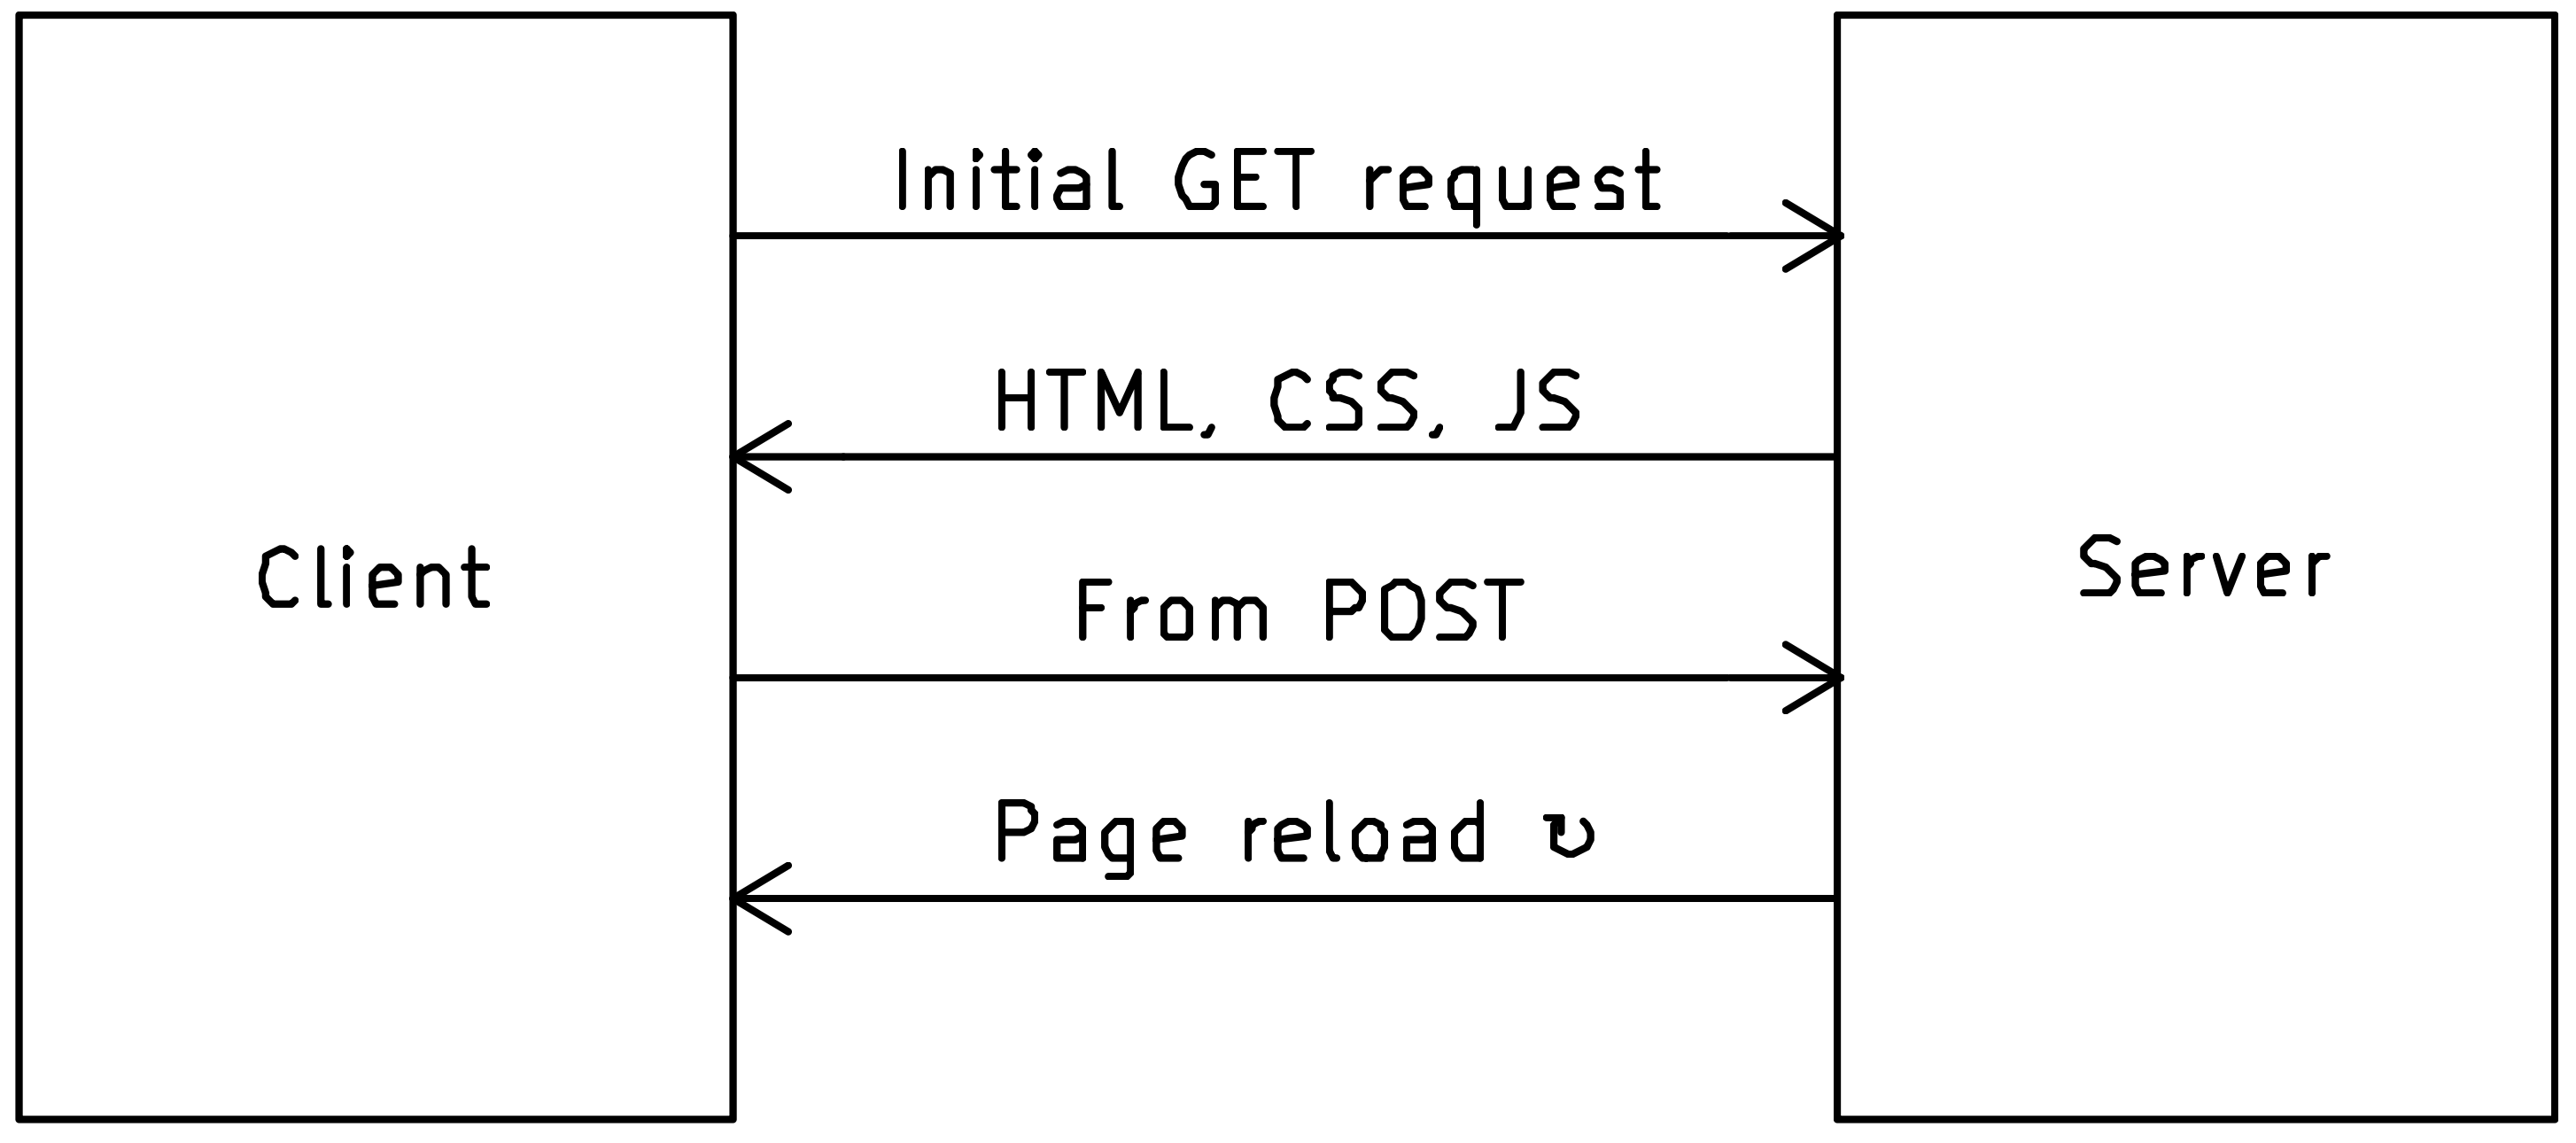
\includegraphics[width=4in]{figures/kicad-mpa-architect.png} % Adjust the image width as needed
            \caption{Back-End Architecture Design of AIT Match Platform.}
            \label{fig:mpa}
        \end{figure}
        
        \begin{figure}[h]
            \centering
            \captionsetup{justification=centering, singlelinecheck=false, labelsep=space}
            
\includegraphics[width=6in]{figures/stack-design.png} % Adjust the image width as needed
            \caption{Back-End Stack Design of AIT Match Platform, including, Rails, Ruby, PostgreSQL, HTML, CSS, Javascript, and Docker.}
            \label{fig:stack}
        \end{figure}   
%-----------------------------------------------%
    \newpage
    \subsection{Back-End Database Design}
        The database efficiently manages all user and admin data, facilitating secure and meaningful connections. The primary entities in the system include:
        
        \begin{enumerate}
            \item \textbf{Users:} The \textit{Users} table stores essential information for user authentication and management, such as email, encrypted passwords, reset password details, and user roles. This table has a one-to-one relationship with the \textit{Profiles} table, allowing each user to have a single associated profile. Additionally, it has a many-to-many relationship with the \textit{Matches} table, enabling users to connect with multiple other users.
        
            \item \textbf{Profiles:} The \textit{Profiles} table contains detailed user-specific information, such as first name, last name, username, MBTI type, gender, degree, school, program, educational background, and birthday. It holds a one-to-one relationship with the \textit{Users} table and a many-to-many relationship with the \textit{Interests} table through the \textit{Profile\_Interests} join table. This structure allows users to showcase their personal and academic details within the system.

            \item \textbf{Active Storage:} The application uses Active Storage to handle file uploads, specifically for user profile pictures. This implementation involves three tables:
                \begin{enumerate}
                    \item \textbf{active\_storage\_attachments:} This table tracks the relationship between records (such as profiles) and the files attached to them. Each entry corresponds to an attachment.
                    \item \textbf{active\_storage\_blobs:} This table stores the actual files and their metadata, including filename and content type.
                    \item \textbf{active\_storage\_variant\_records:} This table manages variants of uploaded files, which can be used to create different versions (like thumbnails) of the images.
                \end{enumerate}
        
            \item \textbf{Genders, Degrees, Schools, Programs, MBTI:} These preset tables store standardized values for user attributes such as gender, degree, school, program, and MBTI type. They are associated with the \textit{Profiles} table, ensuring that users can select these attributes consistently during profile creation and updates, thereby maintaining structured and uniform data across the platform.
        
            \item \textbf{Profile\_Interests:} This join table manages the many-to-many relationship between \textit{Profiles} and \textit{Interests}. It links user profiles to their selected interests, which are stored in the \textit{Interests} table. By storing user preferences in this way, the system can enhance matchmaking by aligning users based on shared hobbies or interests.
        
            \item \textbf{Profile\_Relationships:} The \textit{Profile\_Relationships} table facilitates a many-to-many relationship between user profiles and predefined relationship types from the \textit{Relationships} table. This structure allows users to specify their preferred types of relationships, enriching the platform's ability to match users based on compatible preferences.
        
            \item \textbf{Interests:} The \textit{Interests} table contains a predefined list of interests from which users can choose. It establishes a many-to-many relationship with \textit{Profiles} through the \textit{Profile\_Interests} table. This connection helps the system to accurately match users who share similar interests, improving the overall relevance of suggested profiles.
        
            \item \textbf{Relationships:} The \textit{Relationships} table stores predefined relationship preferences. It is linked to the \textit{Profiles} table via the \textit{Profile\_Relationships} table, enabling users to indicate the types of relationships they are seeking and improving the system’s ability to create meaningful matches.
        
            \item \textbf{Preferences:} The \textit{Preferences} table has a one-to-one relationship with the \textit{Users} table and stores users' filtering preferences, such as preferred age range and relationship types. It is linked to various tables, including \textit{PreferredGenders}, \textit{PreferredDegrees}, \textit{PreferredSchools}, \textit{PreferredPrograms}, \textit{PreferredMBTIs}, and \textit{PreferredRelationships}, allowing users to define specific preferences for potential matches.
            
            \item \textbf{PreferredGenders, PreferredDegrees, PreferredSchools, PreferredPrograms, PreferredMBTIs, PreferredInterests, PreferredRelationships:} These tables store user preferences in categories such as gender, degree, school, program, MBTI type, interests, and relationship types. They establish many-to-many relationships with the \textit{Users} table, contributing to the system’s filtering and matchmaking capabilities by aligning users with others based on their preferred attributes.
        
            \item \textbf{Matches:} The \textit{Matches} table facilitates a many-to-many relationship between users, represented by the requestor and receiver profiles. When two users mutually accept each other, a match is created, allowing them to communicate through the system. This table also tracks the status of match requests, indicating whether a match is pending or confirmed.
        
            \item \textbf{Conversations:} The \textit{Conversations} table stores communication between matched users. Each conversation is associated with a match and involves two profiles, corresponding to the sender and receiver. This structure ensures that all messages between matched users are appropriately organized and tracked.
        
            \item \textbf{Messages:} The \textit{Messages} table is linked to \textit{Conversations} and stores individual messages exchanged between users. It contains fields such as the message content, the sender profile, and timestamps, ensuring a detailed history of all communications between matched users.

           \item \textbf{Reports:} The \textit{Reports} table is associated with the \textit{Profiles} table and stores reports submitted by users regarding other profiles. It includes fields such as reporter\_profile\_id, identifying the user who submitted the report, reported\_profile\_id, identifying the user being reported, reason, detailing the justification provided by the reporter, and status, indicating the current state of the report (“pending” or “reviewed”). This structure enables system administrators to efficiently track, review, and manage user reports, ensuring a safe and respectful platform environment.
        \end{enumerate}

        The ER diagram depicting the back-end database design is presented in Fig. \ref{fig:er-diagram} \href{https://drive.google.com/file/d/1lU1P8GRHPZu2EbJHOeeWxCCiQLVHy9oV/view?usp=sharing}{(see this link for the diagram)}. A more detailed version can be found in Fig. \ref{fig:detailed-er-diagram} \href{https://drive.google.com/file/d/1u3mAT54PdHx2mOwaZDrvpfvSL_J-zFSM/view?usp=drive_link}{(see this link for the detailed diagram)}.

        \begin{figure}[h]
            \centering
            \captionsetup{justification=centering, singlelinecheck=false, labelsep=space}
            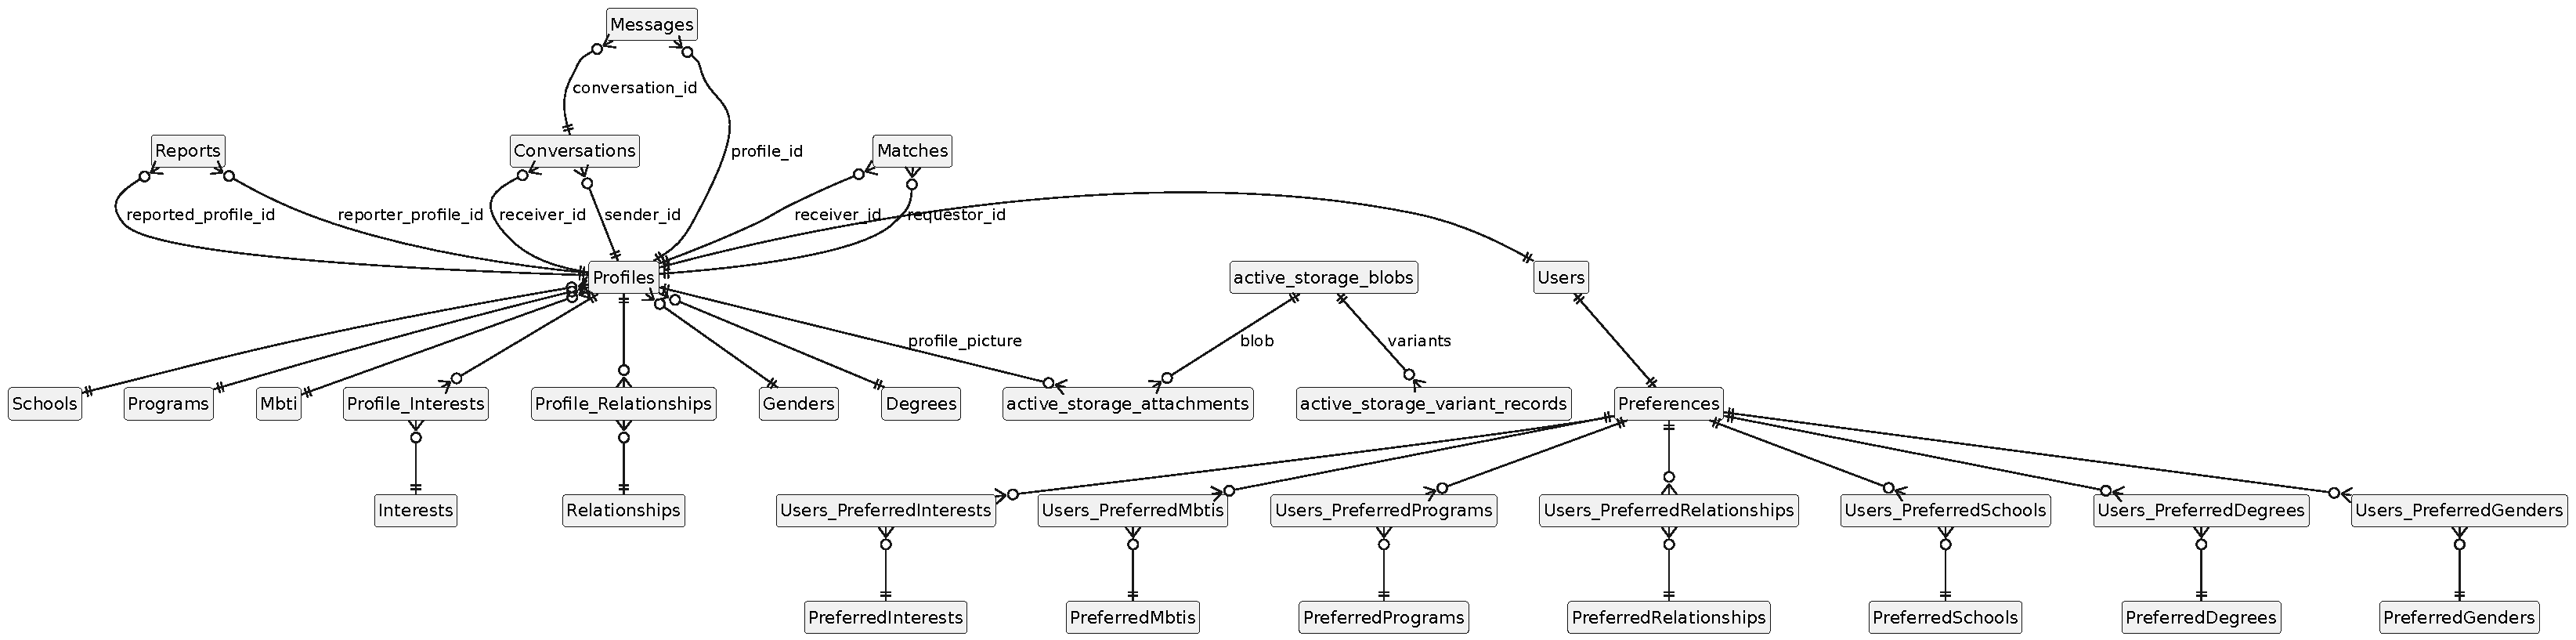
\includegraphics[width=5in]{figures/er-diagram/er-diagram.pdf} % Adjust the image width as needed
            \caption{Back-End Database Design of AIT Match Platform.}
            \label{fig:er-diagram}
        \end{figure}
        
        \begin{figure}[h]
            \centering
            \captionsetup{justification=centering, singlelinecheck=false, labelsep=space}
            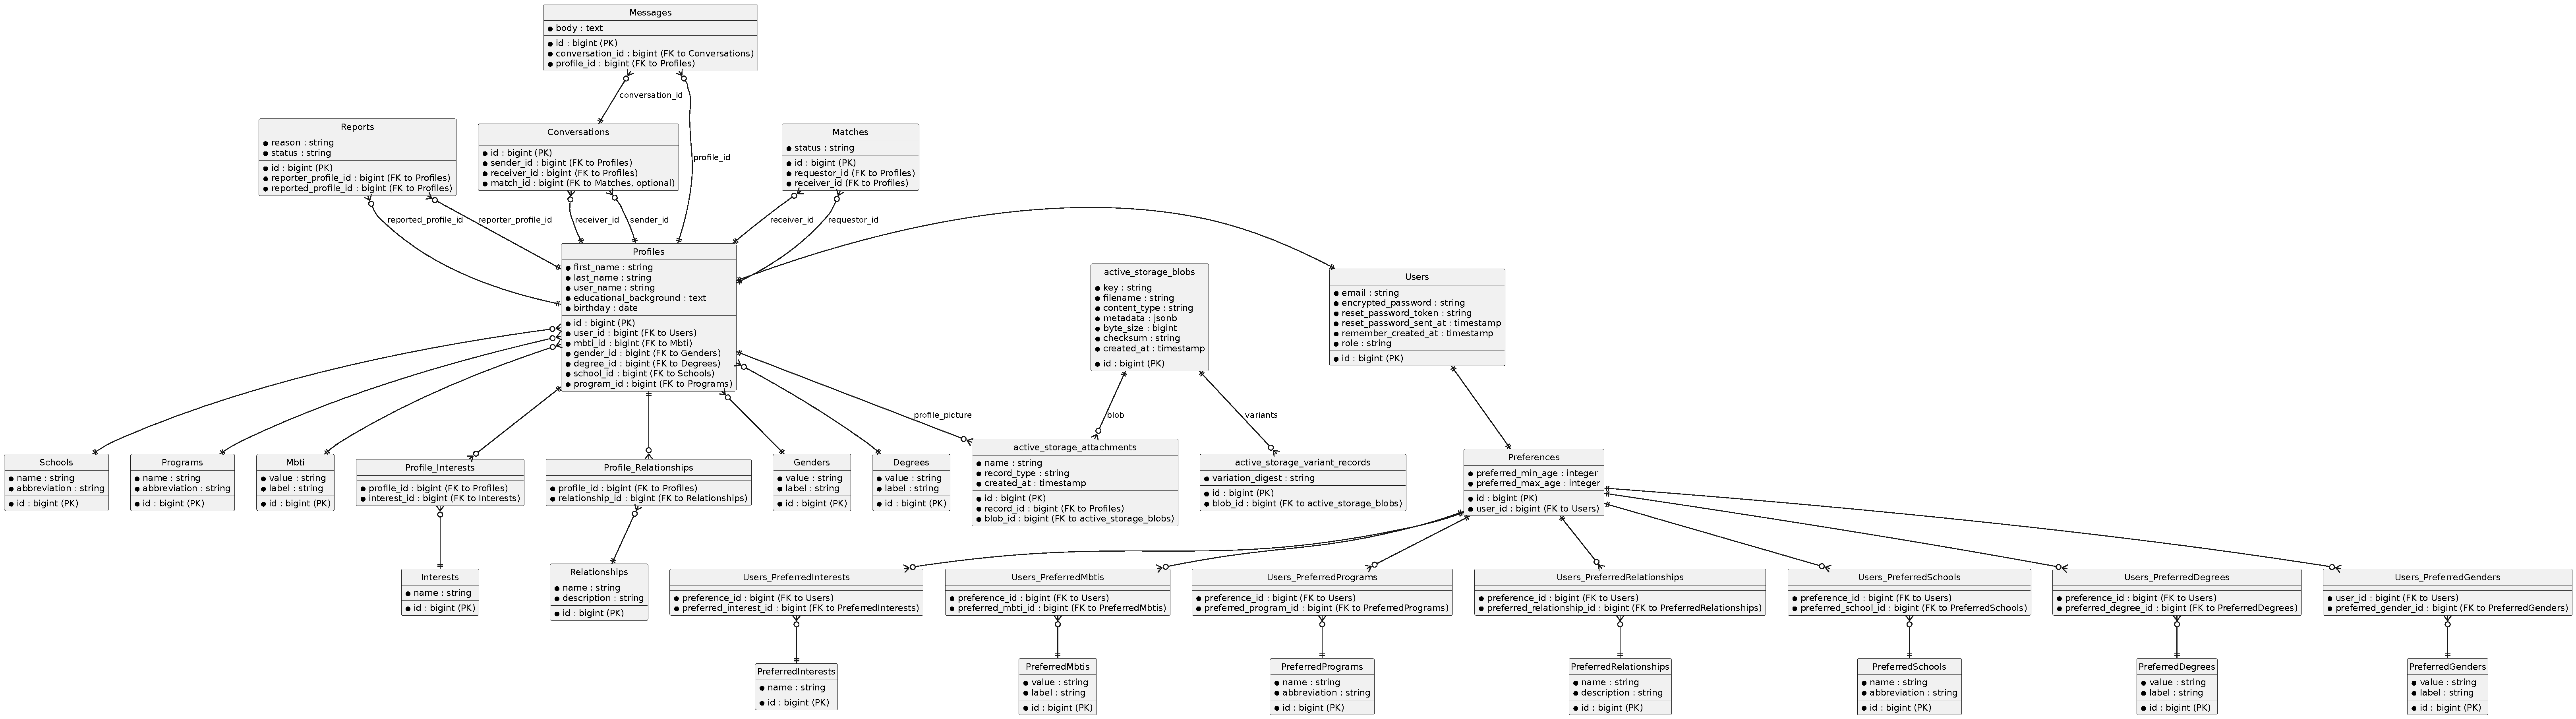
\includegraphics[width=5in]{figures/er-diagram/detailed-er-diagram.pdf} % Adjust the image width as needed
            \caption{Detailed Back-End Database Design of AIT Match Platform.}
            \label{fig:detailed-er-diagram}
        \end{figure}  

%-----------------------------------------------%
    % Change bullet points from dots to dashes
    \setlist[itemize,1]{label=---}
    \newpage
    \subsection{Front-End User Interface Design}
    \begin{enumerate}
        \item \textbf{User Interface Design and Color Palette:}
        The user interface (UI) was designed with a focus on real-world usability and user experience (UX). The goal was to make the application intuitive and easy to use across all platforms. Ruby on Rails uses `.html.erb` files to generate dynamic views, which incorporate both HTML for structuring the web pages and CSS for styling. This combination ensures that the front-end is both functional and visually appealing, allowing for consistent and responsive user interactions.
    
        The color scheme of the website is inspired by tones that create a balanced, safe, and welcoming environment. The green color, derived from the university's branding, represents trustworthiness and security, making users feel comfortable using the platform. Soft pink tones are used to encourage romantic interactions subtly and add warmth to the user experience. The white and grey tones provide a neutral contrast that keeps the interface clean, readable, and visually balanced. The AIT Match color palette is illustrated in Fig. \ref{fig:pantone}.
    
            \begin{figure}[h]
            \centering
            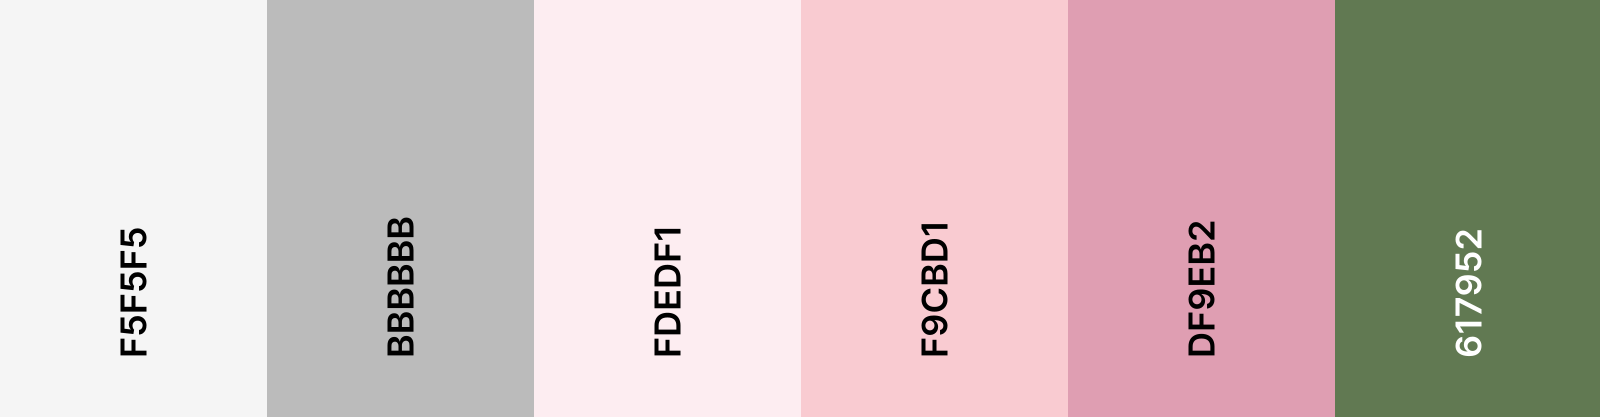
\includegraphics[width=4in]{figures/pantone.png} 
            \captionsetup{justification=centering, singlelinecheck=false, labelsep=space}
            \caption{AIT Match color palette.}
            \label{fig:pantone}
            \end{figure} 

        \item \textbf{Navigation Bar:}
        \begin{itemize}
            \item The logo is prominently displayed.
            \item \textbf{Landing Page Navigation Bar:} Includes buttons for the about page, contact page, login page, and sign-up page.
            \item \textbf{User Navigation Bar:} Includes buttons for home, profile, preferences, matches, messages, and logout.
            \item \textbf{Admin Navigation Bar:} Includes buttons for dashboard, reports, and logout.
        \end{itemize}

        \newpage
        \item \textbf{Login/Sign-up Page:} Allows users to log in or sign up using their university email and password.
        
        \item \textbf{Landing Page:} 
        \begin{itemize}
            \item \textbf{About Page:} Displays information and an overview of the platform.
            \item \textbf{Contact Page:} Provides the contact information for the developers.
        \end{itemize}
        
        \item \textbf{Users’ Main Page:}
        \begin{itemize}
            \item \textbf{Home Page:} Displays all profiles and filtered profiles. Users can match with other users and view profiles.
            \item \textbf{Profile Page:} Allows users to view and edit their profiles.
            \item \textbf{Preference Page:} Allows users to set their preferences to filter other profiles on the home page based on basic information, personality traits, and academic information.
            \item \textbf{Matches Page:} Displays profiles of users who have already matched with the current user.
            \item \textbf{Messages Page:} Shows the latest messages exchanged with matched profiles.
            \item \textbf{Report Page:} Users can report inappropriate profiles to the admin with a detailed reason for each report. The report status will be updated by the admin after review. Users can view their report history but do not have the right to delete any reports.
            \item \textbf{Logout Button:} Logs the user out of the system and redirects them to the login/sign-up page.
        \end{itemize}

        \item \textbf{Admin’s Main Page:}
        \begin{itemize}
            \item \textbf{Dashboard Page:} Displays all user profiles in the system. The admin has the ability to delete profiles as necessary.
            \item \textbf{Report Page:} Shows all reports submitted by users. The admin reviews each report, updates the status accordingly, and has the authority to delete reports, which users cannot do.
            \item \textbf{Logout Button:} Logs the user out of the system and redirects them to the login/sign-up page.
        \end{itemize}
    \end{enumerate}
%-----------------------------------------------%
    \newpage
    \section{System Development}
%-----------------------------------------------%
    \subsection{Environment Setup}
    The AIT Match project uses Ruby on Rails with Docker to streamline development and deployment. Docker ensures consistency across different environments (development, production, etc.). This architecture ensures isolated, reproducible development environments, minimizing environment-specific issues and improving the deployment process. The key components of the environment setup are as follows:
    
    \begin{enumerate}
        \item \textbf{Database Configuration:} 
        The \texttt{database.yml} file configures the PostgreSQL database connection, specifying the adapter, host, username, and password. It ensures that Rails can communicate with the database in both development and production environments, integrating seamlessly with the Docker PostgreSQL container.
    
        \item \textbf{Docker Compose for Database:} 
        Docker Compose orchestrates multiple containers, including the PostgreSQL database (\texttt{match\_db}) and PgAdmin (\texttt{match\_pgadmin}). The services are connected via an internal network (\texttt{match\_network}) for communication. Volumes are used to persist data across container restarts, ensuring database state retention.
    
        \item \textbf{Docker Compose for Rails Application:} 
        Docker Compose also manages the Rails application container (\texttt{match\_web}) and its dependencies like Redis. The Rails service is set up using a Dockerfile and commands to manage the database and precompile assets. Environment variables configure external services, such as Gmail for email notifications and Redis for caching. Redis runs in a separate container and links to the Rails container via the internal network, ensuring persistent data and consistent environments for development and production.
    \end{enumerate}
%-----------------------------------------------%
\newpage
\subsection{User Authentication}
After the environment setup is completed, the next step is to implement user authentication. This is critical to manage access control, allowing only authorized users to log in, register, or reset their passwords securely.

\begin{enumerate}
    \item \textbf{Add Devise and Necessary Gems for Authentication}

    The first task is to add the Devise gem to the Rails application, which provides a complete solution for handling user authentication.

    \begin{itemize}
        \item Install the required gems for authentication:
        \begin{enumerate}
            \item \textbf{\citeauthor{devise2024}:} A flexible authentication solution for Rails applications.
            \item \textbf{\citeauthor{bcrypt2024}:} Used for secure password encryption.
            \item \textbf{\citeauthor{ormadapter2024}, \citeauthor{railties2024}, \citeauthor{warden2024}:} Additional libraries for interacting with the ORM and ensuring authentication logic and security.
        \end{enumerate}

        \item After adding these gems to the \texttt{Gemfile}, run \texttt{bundle install} to install them inside the container.

        \item Generate the Devise configuration and user model using the following commands:
\begin{lstlisting}
        ./bin/rails generate devise:install
        ./bin/rails generate devise User
\end{lstlisting}
    \end{itemize}

    \item \textbf{Validations for Secure User Authentication}

    To ensure the integrity of the registration and login process, validation rules are applied to the Devise model. The following steps ensure that users provide valid information when registering and logging in:

    \begin{enumerate}
        \item \textbf{Email Validation:} Ensure that users can only register using university-provided email addresses. The following validation enforces this format:

\begin{lstlisting}
validates :email, format: { with: /\Ast\d{6}@ (ait.ac.th|ait.asia)\z/, message: "must follow AIT format" }
\end{lstlisting}

        \item \textbf{Password Validation:} Passwords must be at least six characters long and must not be blank:
\begin{lstlisting}
          config.password\_length = 6..128
\end{lstlisting}

        \item \textbf{Unique Email Validation:} Devise automatically ensures that no two users can register with the same email, preventing duplicate accounts.

        \item \textbf{Default Devise Modules:} The following Devise modules are included for user authentication and password recovery:
\begin{lstlisting}
devise  :database_authenticatable, :registerable, 
        :recoverable, :rememberable, :validatable
\end{lstlisting}
    \end{enumerate}

    \item \textbf{User Registration and Database Schema}

    The registration information for users is stored in the \texttt{users} table. The table is generated using a migration file provided by Devise, which is responsible for creating the necessary fields for authentication, password recovery, and other features.

    \begin{enumerate}
        \item \textbf{email}: A string field that stores the user's email address. This is the unique identifier for each user in the system, and it cannot be null or left blank.
        \item \textbf{encrypted\_password}: A string field that stores the encrypted version of the user's password. This field is mandatory and cannot be blank.
        \item \textbf{reset\_password\_token}: A string field used to store the token for password reset functionality. This token is used to verify the identity of users when they request to reset their password.
        \item \textbf{reset\_password\_sent\_at}: A timestamp indicating when the password reset token was sent to the user. This helps ensure that password reset requests expire after a certain period of time.
        \item \textbf{remember\_created\_at}: A timestamp used for the "remember me" functionality, which allows users to stay logged in across sessions.
        \item \textbf{timestamps}: These fields include \texttt{created\_at} and \texttt{updated\_at}, which store the time of creation and the last update of the user's record, respectively.\\
    \end{enumerate}

    Additionally, indexes are added to the \texttt{email} and \texttt{reset\_password\_token} fields to ensure uniqueness and improve query performance.
    As shown in Table \ref{tab:user_schema}, the user schema includes fields for storing user information securely.
    
\begin{table}[h!]
\captionsetup{justification=centering, singlelinecheck=false, labelsep=space}
\centering
\begin{tabular}{ll} % No vertical lines here
\hline
\textbf{Field}               & \textbf{Data Type}                 \\ \hline
id                           & [PK] bigint                        \\ 
email                        & character varying                  \\ 
encrypted\_password          & character varying                  \\ 
reset\_password\_token       & character varying                  \\ 
reset\_password\_sent\_at    & timestamp without time zone (6)    \\ 
remember\_created\_at        & timestamp without time zone (6)    \\ 
created\_at                  & timestamp without time zone (6)    \\ 
updated\_at                  & timestamp without time zone (6)    \\ 
role                         & character varying                  \\ \hline
\end{tabular}
\caption{Users Table Schema} % This should display the caption inline with the label
\label{tab:user_schema} % Add a label here
\end{table}


    \newpage
    \item \textbf{Redirection After Login and Password Reset}

    \begin{enumerate}
        \item After users log in successfully, they are redirected to the \texttt{root\_path}, where they can access their main page.

        \item Users can reset their password by email. The system uses \citeauthor{smtp2024} or Simple Mail Transfer Protocol to send password reset instructions. To enable this, the following configuration is added to \texttt{development.rb} and \texttt{production.rb}:

\begin{lstlisting}
    config.action_mailer.smtp_settings = 
                {...SMTP configuration...}
\end{lstlisting}

    \end{enumerate}

    \item \textbf{SMTP Configuration with Docker Compose}
    To ensure email notifications for password reset and other features, configure SMTP settings in the Docker Compose file. Add Gmail credentials as environment variables:
\begin{lstlisting}
    environment:
        - GMAIL_USERNAME=your-email@gmail.com
        - GMAIL_APP_PASSWORD=your-google-app-password
\end{lstlisting}
    This configuration allows the Rails application to send password reset emails through Gmail’s SMTP service.
    
    \newpage
    \item \textbf{Front-End Views}
    A simple and user-friendly front-end is essential for the user authentication process. The following components are designed using HTML and CSS:

    \begin{enumerate}
        \item \textbf{Login and Sign-Up Forms:} These forms, generated by Devise, allow users to log in or sign up using their university email and password. Users who forget their password can click a link to reset it. The sign-up form is located at devise/registrations/new.html.erb, and the login form is located at \texttt{devise/sessions/new.html.erb}.
        
        \item \textbf{Password Reset Form:} This form allows users to request password reset instructions by entering their registered email address. The password reset form is located at devise/passwords/new.html.erb, and the password edit form (for entering a new password after receiving reset instructions) is located at \texttt{devise/passwords/edit.html.erb}.
        
        \item \textbf{Validation Errors:} Displays clear error messages when users attempt to sign up with invalid email formats or weak passwords. All preset error messages generated by Devise are configured in \texttt{app/config/locales/devise.en.yml}.
    \end{enumerate}
\end{enumerate}
%-----------------------------------------------%
\clearpage
\subsection{Landing Page}
The landing page serves as the introductory section of the AIT Match platform, designed to provide essential information to both new and returning users. To implement the landing page, three controllers and views are generated to handle the different sections: Welcome Page, About Page, and Contact Page.

\begin{enumerate}
    \item \textbf{Back-End Controllers:} 
    To manage each section, the following controllers are generated:
    \begin{itemize}
        \item \textbf{WelcomePageController}: Handles the logic and view for the welcome page.
        \item \textbf{AboutPageController}: Manages the view displaying an overview of the AIT Match website.
        \item \textbf{ContactPageController}: Displays the contact details of the developer for support or inquiries.
    \end{itemize}\bigskip
    
    \item \textbf{Front-End Views:} 
    These pages are implemented using \texttt{.html.erb} files in Rails, incorporating basic HTML and CSS to display information, with no complex back-end logic involved. The goal is to create simple yet informative views that effectively communicate the platform's purpose and make it easy for users to navigate and interact with the website.
    
    \begin{itemize}
        \item \textbf{Welcome Page:} The welcome page greets users and provides a brief explanation of the AIT Match platform. It aims to engage visitors by showing the total number of users who have joined the website, encouraging new users to register and participate. The view is located \texttt{welcome\_page/index.html.erb}.
    
        \item \textbf{About Page:} The about page provides an overview of the AIT Match platform, its goals, and how it facilitates meaningful connections between students. This page is intended for users to understand the core purpose of the platform and its unique features. The view is located \texttt{about\_page/index.html.erb}.
    
        \item \textbf{Contact Page:} The contact page contains the contact information for the developer or support team. It provides users with the necessary details to reach out for help, report issues, or offer suggestions for improving the platform. The view is located in \texttt{contact\_page/index.html.erb}.
    \end{itemize}\bigskip

\end{enumerate}
%-----------------------------------------------%
\subsection{Navigation Bar}
To provide a seamless navigation experience for users, three distinct navbars are created for the AIT Match platform, depending on the user’s role and login status: one for general users before logging in, one for regular users after logging in, and one specifically for admins after logging in.

\begin{itemize}
    \item \textbf{Navigation Bar for Welcome Pages:} 
    This navigation bar is designed for users who have not yet logged in or registered. It includes links to essential pages including ”Home”, “About”, and “Contacts”, allowing visitors to explore basic information about the platform. There are also clear “Log In” and “Sign Up” buttons to encourage new users to join the platform or log in to their existing accounts. The logo is displayed on the left to maintain brand visibility. This navigation bar is located in \texttt{layouts/\_navbar\_welcome\_page.html.erb}.
    

    \item \textbf{Navigation Bar for Users:} 
    Once a user is logged in, the main navigation bar is shown. This provides access to more personalized sections of the platform, such as “Home”, “Profile”, “Preferences”, “Matches”, “Messages”, and “Reports”. Depending on the user's profile and preferences, the links dynamically adjust—for instance, showing a “Create Profile” button if the user hasn’t completed their profile yet. There’s also a “Match Requests” icon to alert users of new match requests. The “Log Out” button is also prominently displayed for easy access. This navigation bar is located in \texttt{layouts/\_navbar.html.erb}.

    \item \textbf{Navigation Bar for Admins:} 
    Upon logging in, admins are presented with a dedicated navigation bar designed for managing users and handling reports. This navigation bar includes three main buttons: “Dashboard” for user management, “Reports” for overseeing user-reported issues, and a prominently displayed “Log Out” button for convenient access. The admin navigation bar is located in \texttt{layouts/\_navbar\_admin.html.erb}.

    \item\textbf{Footer:} At the bottom of all navbars, a simple footer is included across both the welcome pages and the logged-in user pages. The footer displays the text “AIT Match © 2024”, ensuring consistency and providing a clean, professional touch to the website's branding throughout the platform.
\end{itemize}
%-----------------------------------------------%
\newpage
\subsection{Profiles}
\begin{enumerate}
    \item \textbf{Preset Data for Profile Creation:} 
    To ensure consistency and ease of use, dropdown selections are provided for various fields in the profile creation form. These presets include options from tables such as Degree, Gender, Interest, MBTI, Program, Relationship, and School. A new \texttt{presets} table is created to store these options for each of them, meaning that every table has its own preset table for storing preset data from which users can select to create their profiles. Additionally, the Docker Compose file is configured to automatically seed the data every time the Docker environment is restarted. 

    \bigskip
    The dataset used for seeding this data is specified within the \texttt{seeds.rb} file, accessible at the following link:
    \href{https://raw.githubusercontent.com/werrnnnwerrrnnnnnn/AIT-Match/29f98b79013186116728a6cc8f13855453c216bd/app/db/seeds.rb}{Seed Dataset Raw File}.

    \item \textbf{Profile Access Control:} 
    To ensure users are authenticated before accessing any pages, a \texttt{`before\_action :authenticate\_user!'} filter is implemented in the application controller. This ensures that only logged-in users can navigate the website. Additionally, users are required to complete their profiles before accessing other pages on the platform. This is achieved through a custom filter \texttt{`before\_action :check\_profile\_completion'}, which checks if the user’s profile is completed. If a profile does not exist, the system redirects the user to the profile creation page with an alert message.
    \begin{lstlisting}
    before_action :authenticate_user!
    before_action :check_profile_completion
    
    private
    def check_profile_completion
      if current_user.profile.nil?
        flash[:alert] = "Please complete your profile before accessing this page."
        redirect_to new_profile_path
      end
    end
    \end{lstlisting}

    \newpage
    \item \textbf{Profile Create:} 
    After logging into the system for the first time, users are required to create a profile before accessing any other pages. The profile creation form includes fields for first name, last name, username, birthday, and other academic and personal details, such as MBTI, gender, degree, school, and program. There are also sections for interests and preferred relationship types, where users can select multiple options. Each field in the profile creation form is validated to ensure data correctness, such as unique usernames and mandatory fields like first name, last name, and email.
    \begin{lstlisting}
    def create
        @profile = Profile.new(profile_params)
        @profile.user = current_user
      
        if @profile.save
          redirect_to @profile, notice: 'Profile was successfully created.'
        else
          # Render the new template with errors
          render :new, status: :unprocessable_entity
        end
    end
    \end{lstlisting}

    \item \textbf{Profile New:}
    After logging in, users who have not yet created a profile are prompted to do so. If a user attempts to create a profile again after already having one, the system prevents this action, as each user is allowed only a single profile.
    \begin{lstlisting}
    def new
        if current_user.profile.present?
          flash[:alert] = 'You already have a profile. Please edit your existing profile.'
          redirect_to profile_path(current_user.profile)
        else
          @profile = Profile.new
        end
    end
    \end{lstlisting}

    \newpage
    \item \textbf{Profile Edit:} 
    Once the profile is successfully created, users can access other sections of the platform. The profile can be viewed and edited at any time. Users can update their details, add new interests, or change preferences such as relationship types. The system ensures that each update is validated for correctness.
    \begin{lstlisting}
    def edit
        @profile = current_user.profile
    end
    \end{lstlisting}

    \item \textbf{Profile Update:} 
    After editing the profile, the system updates the information in the database. A success message is shown, and the user is redirected back to their profile page.
    \begin{lstlisting}
    def update
        @profile = current_user.profile
      
        if @profile.update(profile_params)
          redirect_to @profile, notice: 'Profile was successfully updated.'
        else
          # Render the edit template with errors
          render :edit, status: :unprocessable_entity
        end
    end
    \end{lstlisting}

    \newpage
    \item \textbf{Profile Show:} 
    Users can view their complete profile information in a dedicated “Profile” section, which includes personal details, academic background, interests, and preferences. Current users can view both their own profile and the profiles of other users.
    \begin{lstlisting}
def show
    @profile = Profile.find_by(id: params[:id])
    if @profile.nil?
      redirect_to profiles_path, alert: "Profile not found."
    else
      @interests = @profile.interests
      @user = @profile.user
    end
end
    \end{lstlisting}

    \newpage
    \item \textbf{Profile Delete:} 
    Users can delete their profile, but to prevent accidental deletions, the system requires users to confirm their username before proceeding with deletion. The user must enter their username correctly, and if the entered username does not match, the system will display an error message and prevent the profile from being deleted.
    \begin{lstlisting}
def destroy
    if @profile.destroy
      redirect_to root_path, notice: 'Profile was successfully deleted.'
    else
      redirect_to profile_path(@profile), alert: 'Something went wrong. Unable to delete profile.'
    end
end
    \end{lstlisting}

\begin{lstlisting}
<script>
document.addEventListener("DOMContentLoaded", function() {
    const form = document.getElementById("profileDeletionForm");

    form.addEventListener("submit", function(event) {
        const usernameInput = event.target.querySelector("input[name='username']");
        const enteredUsername = usernameInput.value;
        const currentUsername = "<%= current_user.profile.user_name %>";

        if (enteredUsername !== currentUsername) {
            alert("Username does not match. Please type your correct username.");
            event.preventDefault(); // Prevent form submission
        }
    });
});
</script>
\end{lstlisting}

    \newpage
    \item \textbf{Profile Index:} 
    The system provides several key functionalities for profile management, including the ability to search profiles, filter by preferences, and view specific profiles. Users can edit their profile through an intuitive interface, and sorting options (A-Z, Z-A, or random) allow for flexibility in how profiles are displayed. Profiles can be viewed by others, and notifications are shown when matches or messages are received.
    \begin{lstlisting}
def index
    # Fetch all profiles, excluding the current user's own profile
    @profiles = Profile.where.not(user: current_user)
  
    # Initialize @filtered_profiles as all profiles
    @filtered_profiles = @profiles

    # Check if filtering should be disabled (via disable_filters parameter)
    if params[:disable_filters].present?
      # Skip applying filters
      @filtering_disabled = true
    else
      # Apply filters only if the user has set preferences and no sorting is applied
      if current_user.preference.present?
        apply_filters(current_user.preference)
        @filtering = true
    end
end
\end{lstlisting}

    \newpage
    \item \textbf{Profile Database Schema:}
    The profile information for users is stored in the \texttt{profiles} table. The table is generated to hold important user profile details such as academic background, MBTI type, and profile picture. Below is an explanation of the fields in this table:

    \begin{enumerate}
        \item \textbf{id}: A primary key (bigint) that uniquely identifies each profile record.
        \item \textbf{user\_id}: A foreign key (bigint) linking each profile to the corresponding user.
        \item \textbf{first\_name}: A string field storing the user's first name.
        \item \textbf{last\_name}: A string field storing the user's last name.
        \item \textbf{user\_name}: A unique string field for the user's username, used for identifying them within the system.
        \item \textbf{mbti\_id}: A foreign key (bigint) linking to the MBTI type in the MBTI table.
        \item \textbf{gender\_id}: A foreign key (bigint) linking to the gender type in the Genders table.
        \item \textbf{degree\_id}: A foreign key (bigint) linking to the degree type in the Degrees table.
        \item \textbf{school\_id}: A foreign key (bigint) linking to the school information in the Schools table.
        \item \textbf{program\_id}: A foreign key (bigint) linking to the program information in the Programs table.
        \item \textbf{educational\_background}: A text field storing additional information about the user's educational background.
        \item \textbf{created\_at}: A timestamp storing when the profile was first created.
        \item \textbf{updated\_at}: A timestamp storing the most recent update time of the profile.
        \item \textbf{birthday}: A date field storing the user's birthday.\\
    \end{enumerate}

    Additionally, indexes are added to some fields like \texttt{user\_id} to optimize queries and enforce uniqueness.

    \begin{table}[h!]
    \centering
    \begin{tabular}{lcc}
        \hline
        \textbf{Field}               & \textbf{Data Type}                 \\ \hline
        id                           & [PK] bigint                        \\ 
        user\_id                     & bigint                             \\ 
        first\_name                  & character varying                  \\ 
        last\_name                   & character varying                  \\ 
        user\_name                   & character varying                  \\ 
        mbti\_id                     & bigint                             \\ 
        gender\_id                   & bigint                             \\ 
        degree\_id                   & bigint                             \\ 
        school\_id                   & bigint                             \\ 
        program\_id                  & bigint                             \\ 
        educational\_background      & text                               \\ 
        created\_at                  & timestamp without time zone (6)    \\ 
        updated\_at                  & timestamp without time zone (6)    \\ 
        birthday                     & date                               \\ \hline
    \end{tabular}
    
    \vspace{0.3cm} % Optional: adds a small space between the table and the caption
    \small\centerline{\textit{Table 3.2} Profiles Table Schema} % Caption in the requested style
    \end{table}

    \clearpage
    \subsection{Active Storage for Profile Pictures}
        \bigskip
        Active Storage is utilized in the AIT Match application to handle user-uploaded files, specifically for storing profile pictures. This feature allows users to easily upload and manage their profile images, enhancing the personalization aspect of the platform. According to \cite{rails_active_storage}, the implementation of Active Storage involves three key tables:
        
        \begin{enumerate}
            \item \textbf{active\_storage\_attachments:} This table keeps track of the relationships between records (in this case, profiles) and the files attached to them. Each entry corresponds to an attachment, storing fields such as:
            \begin{itemize}
                \item \textbf{id}: A primary key that uniquely identifies each attachment.
                \item \textbf{name}: The name of the attachment.
                \item \textbf{record\_type}: The type of the record that the file is associated with, in this case, \texttt{Profile}.
                \item \textbf{record\_id}: The ID of the record that the attachment belongs to.
                \item \textbf{blob\_id}: A foreign key linking to the blob containing the actual file data.
                \item \textbf{created\_at}: A timestamp indicating when the attachment was created.
            \end{itemize}

            \bigskip
            \begin{table}[h!]
            \centering
            \begin{tabular}{lcc}
                \hline
                \textbf{Field}               & \textbf{Data Type}                 \\ \hline
                id                           & [PK] bigint                        \\ 
                name                         & character varying                  \\ 
                record\_type                & character varying                  \\ 
                record\_id                  & bigint                             \\ 
                blob\_id                    & bigint                             \\ 
                created\_at                 & timestamp without time zone (6)    \\ \hline
            \end{tabular}
            
            \vspace{0.3cm} % Optional: adds a small space between the table and the caption
            \small\centerline{\textit{Table 3.2} Active Storage Attachments Table} % Caption in the requested style
            \label{tab:active_storage_attachments}
            \end{table}
        
            \item \textbf{active\_storage\_blobs:} This table stores the actual files and their metadata. Each entry corresponds to a file uploaded by users and contains fields such as:
            \begin{itemize}
                \item \textbf{id}: A primary key for the blob.
                \item \textbf{key}: A unique identifier for the file.
                \item \textbf{filename}: The original name of the uploaded file.
                \item \textbf{content\_type}: The MIME type of the file (e.g., image/png).
                \item \textbf{metadata}: Additional information about the file, such as analysis results.
                \item \textbf{byte\_size}: The size of the file in bytes.
                \item \textbf{created\_at}: A timestamp for when the file was created.
            \end{itemize}

            \bigskip
            \begin{table}[h!]
            \centering
            \begin{tabular}{lcc}
                \hline
                \textbf{Field}               & \textbf{Data Type}                 \\ \hline
                id                           & [PK] bigint                        \\ 
                key                          & character varying                  \\ 
                filename                     & character varying                  \\ 
                content\_type                & character varying                  \\ 
                metadata                     & text                               \\ 
                byte\_size                   & bigint                             \\ 
                created\_at                 & timestamp without time zone (6)    \\ \hline
            \end{tabular}
            
            \vspace{0.3cm} % Optional: adds a small space between the table and the caption
            \small\centerline{\textit{Table 3.3} Active Storage Blobs Table} % Caption in the requested style
            \label{tab:active_storage_blobs}
            \end{table}
        
            \item \textbf{active\_storage\_variant\_records:} This table stores records for variants of the uploaded files, which can be used to create different versions (like thumbnails). It contains:
            \begin{itemize}
                \item \textbf{id}: A primary key for the variant record.
                \item \textbf{blob\_id}: A foreign key linking to the corresponding blob.
                \item \textbf{variation\_digest}: A character varying field that holds the identifier for the variant's configuration.
            \end{itemize}
            
            \bigskip
            \begin{table}[h!]
            \centering
            \begin{tabular}{lcc}
                \hline
                \textbf{Field}              & \textbf{Data Type}                 \\ \hline
                id                          & [PK] bigint                        \\ 
                blob\_id                    & bigint                             \\ 
                variation\_digest           & character varying                  \\ \hline
            \end{tabular}
            
            \vspace{0.3cm} % Optional: adds a small space between the table and the caption
            \small\centerline{\textit{Table 3.4} Active Storage Variant Records Table} % Caption in the requested style
            \label{tab:active_storage_variant_records}
            \end{table}
        \end{enumerate}
        
        The integration of Active Storage ensures that user profile pictures are managed efficiently while maintaining a high level of security and accessibility.

    \newpage
    \item \textbf{Front-End Views:}
    \begin{itemize}
        \item \textbf{Profile New:} After logging into the system, users are required to complete their profile on this page before accessing other parts of the platform. They must fill out all mandatory fields, including First Name, Last Name, unique Username, Birthday, MBTI Type, Gender, Degree, School, Program, Educational Background, and Profile Picture. Additionally, users have the option to select Interests (up to five) and Preferred Relationship types. This comprehensive profile setup ensures that users have sufficient information available on the platform, fostering meaningful connections based on shared interests and preferences. The view is located at \texttt{profiles/new.html.erb}.
    
        
        \item \textbf{Profile Index:} This page displays all profiles in the system, allowing users to view, search, and sort profiles by username, or apply filters based on their preferences. The filtered profiles are shown on the index page, with selected preference details displayed on the sidebar, providing context for the filtered results. Each profile card presents user information and offers options to view the profile in detail or initiate a match request by clicking the buttons. The search bar, sorting dropdown, and filter preferences enable users to customize their browsing experience, enhancing navigation and interaction within platform. The view is located at \texttt{profiles/index.html.erb}.
    
        \item \textbf{Profile Show:} This profile page is accessed when a user views their own profile or another user’s profile. The system checks the profile ID to determine which profile to display. The page includes fields for profile picture, role, name, username, email, birthday, age, gender, MBTI type, degree, school, program, educational background, relationship preferences, and interests. Users can navigate back, report, or edit the profile based on permissions. This organized layout provides quick access to essential profile details. The view is located at \texttt{profiles/show.html.erb}.

        \item \textbf{Profile Edit:} After initially setting up their profile, this page enables users to make edits to previously configured details. Additionally, users have the option to permanently delete their profile by confirming their username, adding a layer of security to the deletion process. This design offers a user-friendly interface for managing and updating profile information effectively. The view is located at \texttt{profiles/edit.html.erb}.
    \end{itemize}\bigskip
    
\end{enumerate}
%-----------------------------------------------%
\clearpage \newpage
\subsection{Preferences}\bigskip

\begin{enumerate}
    \item \textbf{Preferences Preset Data:} 
    Similar to the profile creation process, preset data is provided to facilitate preference selection. These presets allow users to select from predefined categories such as Degree, Gender, Interest, MBTI, Program, Relationship, and School, ensuring a standardized format for filtering profiles. Each preference category is associated with a dedicated table, allowing for the efficient storage and retrieval of user preferences.

    \bigskip
    The dataset used for seeding this data is specified within the \texttt{seeds.rb} file, accessible at the following link:
    \href{https://raw.githubusercontent.com/werrnnnwerrrnnnnnn/AIT-Match/29f98b79013186116728a6cc8f13855453c216bd/app/db/seeds.rb}{Seed Dataset Raw File}.

    \item \textbf{Preference Access Control:} 
    To ensure users are authenticated before accessing any pages, a \texttt{`before\_action :authenticate\_user!'} filter is implemented in the application controller. This ensures that only logged-in users can navigate the website. Additionally, users are required to complete their profiles before accessing other pages on the platform. This is achieved through a custom filter \texttt{`before\_action :check\_profile\_completion'}, which checks if the user’s profile is completed. If a profile does not exist, the system redirects the user to the profile creation page with an alert message.
    \begin{lstlisting}
    before_action :authenticate_user!
    before_action :check_profile_completion
    
    private
    def check_profile_completion
      if current_user.profile.nil?
        flash[:alert] = "Please complete your profile before accessing this page."
        redirect_to new_profile_path
      end
    end
    \end{lstlisting}

    \newpage
    \item \textbf{Preference Storage Structure:} 
    User preferences are stored in a dedicated \texttt{preference} table, along with several many-to-many associated tables to allow multiple selections for each preference type. The associated tables include:
    
    \begin{itemize}
        \item \texttt{users\_preferred\_degree}
        \item \texttt{users\_preferred\_gender}
        \item \texttt{users\_preferred\_interest}
        \item \texttt{users\_preferred\_mbti}
        \item \texttt{users\_preferred\_program}
        \item \texttt{users\_preferred\_relationship}
        \item \texttt{users\_preferred\_school}
    \end{itemize}
    \bigskip This structure allows users to select multiple options for each preference, such as indicating interest in more than one degree or relationship type. For example, the \texttt{UsersPreferredGender} model relates user preferences for gender types to the \texttt{preference} table and the \texttt{PreferredGender} table, following a similar structure across all related tables to accommodate multiple selections:
    \begin{lstlisting}
    class UsersPreferredGender < ApplicationRecord
      belongs_to :preference
      belongs_to :preferred_gender
    end
    \end{lstlisting}

    \item \textbf{Preference New:} 
    After creating a profile, users can proceed to set their preferences. This process involves selecting values for various criteria, such as age range, gender, interests, and relationship types. Each preference selection is validated to ensure consistency and correctness. For example, users can only select options available within the preset data, ensuring the integrity of filterable criteria.

    \begin{lstlisting}
    def new
        @preference = Preference.new
        load_filter_options
    end
    \end{lstlisting}

    \newpage
    \item \textbf{Preference Create:} 
    Once a user creates and saves their preferences, the preference data is stored in the corresponding database, accompanied by a notification message confirming the save action.
    \begin{lstlisting}
    def create
        @preference = current_user.build_preference(preference_params)
        if @preference.save
          redirect_to profiles_path, notice: 'Preferences were successfully set.'
        else
          load_filter_options
          render :new
        end
    end
    \end{lstlisting}

    \item \textbf{Preference Edit:} 
    Users can edit their preferences at any time, continuing from their previously set choices. 
    \begin{lstlisting}
    def edit
        load_filter_options
    end
    \end{lstlisting}

    \item \textbf{Preference Update:} 
    After users edit their preferences and save, the updated data is stored in the database, accompanied by a notification message.
    \begin{lstlisting}
    def update
        if @preference.update(preference_params)
          redirect_to profiles_path, notice: 'Preferences were successfully updated.'
        else
          load_filter_options
          render :edit
        end
    end
    \end{lstlisting}

    \newpage
    \item \textbf{Filtering System:} 
    The primary method responsible for filtering profiles according to user preferences is the \texttt{apply\_filters} function within the \texttt{ProfilesController}. This function takes the \texttt{preference} object containing the user’s selections and applies multiple filters based on the specified criteria.

    \bigskip The filtering process in \texttt{apply\_filters} includes the following steps:
    
    \begin{enumerate}
        \item Initial Setup with \texttt{distinct}: Ensures unique profiles by selecting \texttt{profiles.*} and calling \texttt{.distinct}.
        \item Filtering Criteria:
        \begin{itemize}
            \item Age Range: Filters profiles based on the selected age range.
            \item Gender: Filters by the user’s preferred gender selections.
            \item Interests: Filters by matching interests between profiles.
            \item Relationship Types: Filters by preferred relationship types.
            \item MBTI: Filters based on personality compatibility.
            \item School and Program: Filters profiles by preferred schools and programs.
        \end{itemize}
    \end{enumerate}
    
    \bigskip Each \texttt{if} block within \texttt{apply\_filters} checks if a preference is present before applying the corresponding filter, ensuring that only active preferences are used. This method is called within the \texttt{index} action of the \texttt{ProfilesController} to display profiles filtered according to the user’s preferences, offering a tailored profile viewing experience. Below is the code for the \texttt{apply\_filters} method that performs profile filtering based on user preferences:
    \begin{lstlisting}
private
def apply_filters(preference)
  @filtered_profiles = @filtered_profiles.select('profiles.*').distinct
  
  # Filter by age range
  if preference.preferred_min_age.present? && preference.preferred_max_age.present?
    today = Date.today
    min_birthdate = today.years_ago(preference.preferred_max_age)
    max_birthdate = today.years_ago(preference.preferred_min_age)
    @filtered_profiles = @filtered_profiles.where("birthday >= ? AND birthday <= ?", min_birthdate, max_birthdate)
  end

  # Filter by gender preferences
  if preference.preferred_genders.any?
    @filtered_profiles = @filtered_profiles.joins(:gender).where(genders: { id: preference.preferred_gender_ids })
  end

  # Filter by interest preferences
  if preference.preferred_interests.any?
    @filtered_profiles = @filtered_profiles.joins(:interests).where(interests: { id: preference.preferred_interest_ids })
  end

  # Filter by relationship preferences
  if preference.preferred_relationships.any?
    @filtered_profiles = @filtered_profiles.joins(:relationships).where(relationships: { id: preference.preferred_relationship_ids })
  end

  # Filter by MBTI preferences
  if preference.preferred_mbti.any?
    @filtered_profiles = @filtered_profiles.joins(:mbti).where(mbtis: { id: preference.preferred_mbti_ids })
  end

  ...
    \end{lstlisting}
    
    \newpage
    \item \textbf{Preferences Database Schema:}  
    The preferences information for users is stored in the \texttt{preferences} table. This table holds user-defined filtering criteria, such as age range and other settings, which are used to customize the profile results displayed to each user. Below is an explanation of the fields in this table:

        \begin{enumerate}
            \item \textbf{id}: A primary key (bigint) that uniquely identifies each preferences record.
            \item \textbf{user\_id}: A foreign key (bigint) linking each preference set to the corresponding user.
            \item \textbf{preferred\_min\_age}: An integer field specifying the minimum preferred age for matching profiles.
            \item \textbf{preferred\_max\_age}: An integer field specifying the maximum preferred age for matching profiles.
        \end{enumerate}

\bigskip Additionally, indexes are added to fields like \texttt{user\_id} to optimize query performance and ensure data integrity.
    %-----------------------------------------------%
    \begin{table}[h!]
    \captionsetup{justification=centering, singlelinecheck=false, labelsep=space}
    \centering
    \begin{tabular}{ll} % No vertical lines here
    \hline
    \textbf{Field}               & \textbf{Data Type}                 \\ \hline
    id                           & [PK] bigint                        \\ 
    user\_id                     & bigint                             \\ 
    preferred\_min\_age          & integer                            \\ 
    preferred\_max\_age          & integer                            \\ 
    created\_at                  & timestamp without time zone (6)    \\ 
    updated\_at                  & timestamp without time zone (6)    \\ \hline
    \end{tabular}
    \caption{Preferences Table Schema} % This should display the caption inline with the label
    \label{tab:Preferences Table Schema}
    \end{table}
    %-----------------------------------------------%
    \begin{table}[h!]
    \captionsetup{justification=centering, singlelinecheck=false, labelsep=space}
    \centering
    \begin{tabular}{ll}
    \hline
    \textbf{Field}               & \textbf{Data Type}                 \\ \hline
    id                           & [PK] bigint                        \\ 
    preference\_id               & bigint                             \\ 
    preferred\_degree\_id        & bigint                             \\ 
    created\_at                  & timestamp without time zone (6)    \\ 
    updated\_at                  & timestamp without time zone (6)    \\ \hline
    \end{tabular}
    \caption{Users Preferred Degrees Table Schema}
    \label{tab:Users Preferred Degrees Table Schema}
    \end{table}
    \vspace{2cm} % Adjust the space as needed
    %-----------------------------------------------%
    \begin{table}[h!]
    \captionsetup{justification=centering, singlelinecheck=false, labelsep=space}
    \centering
    \begin{tabular}{ll}
    \hline
    \textbf{Field}               & \textbf{Data Type}                 \\ \hline
    id                           & [PK] bigint                        \\ 
    preference\_id               & bigint                             \\ 
    preferred\_gender\_id        & bigint                             \\ 
    created\_at                  & timestamp without time zone (6)    \\ 
    updated\_at                  & timestamp without time zone (6)    \\ \hline
    \end{tabular}
    \caption{Users Preferred Genders Table Schema}
    \label{tab:Users Preferred Genders Table Schema}
    \end{table}
    \vspace{2cm} % Adjust the space as needed
    %-----------------------------------------------%
    \begin{table}[h!]
    \captionsetup{justification=centering, singlelinecheck=false, labelsep=space}
    \centering
    \begin{tabular}{ll}
    \hline
    \textbf{Field}               & \textbf{Data Type}                 \\ \hline
    id                           & [PK] bigint                        \\ 
    preference\_id               & bigint                             \\ 
    preferred\_interest\_id      & bigint                             \\ 
    created\_at                  & timestamp without time zone (6)    \\ 
    updated\_at                  & timestamp without time zone (6)    \\ \hline
    \end{tabular}
    \caption{Users Preferred Interests Table Schema}
    \label{tab:Users Preferred Interests Table Schema}
    \end{table}
    \vspace{0cm} % Adjust the space as needed
    %-----------------------------------------------%
    \begin{table}[h!]
    \captionsetup{justification=centering, singlelinecheck=false, labelsep=space}
    \centering
    \begin{tabular}{ll}
    \hline
    \textbf{Field}               & \textbf{Data Type}                 \\ \hline
    id                           & [PK] bigint                        \\ 
    preference\_id               & bigint                             \\ 
    preferred\_mbti\_id          & bigint                             \\ 
    created\_at                  & timestamp without time zone (6)    \\ 
    updated\_at                  & timestamp without time zone (6)    \\ \hline
    \end{tabular}
    \caption{Users Preferred MBTIs Table Schema}
    \label{tab:Users Preferred MBTIs Table Schema}
    \end{table}
    \vspace{2cm} % Adjust the space as needed
    %-----------------------------------------------%
    \begin{table}[h!]
    \captionsetup{justification=centering, singlelinecheck=false, labelsep=space}
    \centering
    \begin{tabular}{ll}
    \hline
    \textbf{Field}               & \textbf{Data Type}                 \\ \hline
    id                           & [PK] bigint                        \\ 
    preference\_id               & bigint                             \\ 
    preferred\_program\_id       & bigint                             \\ 
    created\_at                  & timestamp without time zone (6)    \\ 
    updated\_at                  & timestamp without time zone (6)    \\ \hline
    \end{tabular}
    \caption{Users Preferred Programs Table Schema}
    \label{tab:Users Preferred Programs Table Schema}
    \end{table}
    \vspace{2cm} % Adjust the space as needed
    %-----------------------------------------------%
    \begin{table}[h!]
    \captionsetup{justification=centering, singlelinecheck=false, labelsep=space}
    \centering
    \begin{tabular}{ll}
    \hline
    \textbf{Field}               & \textbf{Data Type}                 \\ \hline
    id                           & [PK] bigint                        \\ 
    preference\_id               & bigint                             \\ 
    preferred\_relationship\_id  & bigint                             \\ 
    created\_at                  & timestamp without time zone (6)    \\ 
    updated\_at                  & timestamp without time zone (6)    \\ \hline
    \end{tabular}
    \caption{Users Preferred Relationships Table Schema}
    \label{tab:Users Preferred Relationships Table Schema}
    \end{table}
    \vspace{2cm} % Adjust the space as needed
    %-----------------------------------------------%
    \begin{table}[h!]
    \captionsetup{justification=centering, singlelinecheck=false, labelsep=space}
    \centering
    \begin{tabular}{ll}
    \hline
    \textbf{Field}               & \textbf{Data Type}                 \\ \hline
    id                           & [PK] bigint                        \\ 
    preference\_id               & bigint                             \\ 
    preferred\_school\_id        & bigint                             \\ 
    created\_at                  & timestamp without time zone (6)    \\ 
    updated\_at                  & timestamp without time zone (6)    \\ \hline
    \end{tabular}
    \caption{Users Preferred Schools Table Schema}
    \label{tab:Users Preferred Schools Table Schema}
    \end{table}
    \vspace{2cm} % Adjust the space as needed
    
    The tables presented above store user-defined preferences that enable individuals on the AIT Match platform to filter potential matches based on specific criteria. Each table corresponds to a distinct aspect of user preferences, including degree, gender, interest, MBTI, program, relationship type, and school, and is linked to the main preferences table through foreign keys. This structure allows for flexible and customizable matching, ensuring that users can tailor their connections to align with both personal and academic interests.
    
    \newpage
    \item \textbf{Front-End Views:}
    \begin{itemize}
        \item \textbf{Preference New:} Upon logging into the system, users are prompted to complete their profile on this page before they can access other sections of the platform. After completing their profile setup, users are directed to create their initial preferences by selecting relevant fields, including minimum and maximum age range, preferred genders, MBTI types, degrees, schools, programs, and relationship types. Once the preferences are saved, the data is stored across all related tables in the database. This view is located at \texttt{preferences/new.html.erb}.
    
        
        \item \textbf{Preference Edit:} After setting up their preferences, users can edit them at any time by modifying the same fields available in the initial preference setup. Once the preferences are updated, the new data is saved in the database, replacing the previous entries. This view is located at \texttt{preferences/edit.html.erb}.
    \end{itemize}
\end{enumerate} 
%-----------------------------------------------%
    \newpage 
    \subsection{Matches}
    Two profiles can initiate a match and engage in messaging if both agree to connect. The matching process involves three statuses: pending, accepted, and declined. A user (referred to as the requestor) can send a match request to another user (the receiver) and await their response. If the receiver accepts, the profiles are matched and can start chatting; otherwise, the request is marked as declined.

    \begin{enumerate}
    \item \textbf{Matches Access Control:} 
    To ensure users are authenticated before accessing any pages, a \texttt{`before\_action :authenticate\_user!'} filter is implemented in the application controller. This ensures that only logged-in users can navigate the website. Additionally, users are required to complete their profiles before accessing other pages on the platform. This is achieved through a custom filter \texttt{`before\_action :check\_profile\_completion'}, which checks if the user’s profile is completed. If a profile does not exist, the system redirects the user to the profile creation page with an alert message.
    \begin{lstlisting}
    before_action :authenticate_user!
    before_action :check_profile_completion
    
    private
    def check_profile_completion
      if current_user.profile.nil?
        flash[:alert] = "Please complete your profile before accessing this page."
        redirect_to new_profile_path
      end
    end
    \end{lstlisting}

    \newpage
    \item \textbf{Match Create:} 
    As the requestor, a user can send a match request to another user (the receiver) only if the status of a previous request between them is neither “accepted” nor “pending.” When a match request is created, the system displays a notice to the requestor indicating whether the request was successfully sent or if it failed. The create method first identifies the receiver’s profile using the profile\_id parameter. It then checks for any existing match requests with a “declined” status between the sender and receiver; if such a request exists, it updates the status to “pending,” allowing the request to be resent. If no declined match exists, the method creates a new match request with a “pending” status. Finally, it attempts to save the request, redirecting to the receiver’s profile with a success message upon success or showing an error alert if the request fails.
    \begin{lstlisting}
def create
    # Find the receiver profile using the ID passed from the button
    @receiver = Profile.find(params[:profile_id])
  
    # Check if a match already exists between the current user and the receiver in either direction
    existing_match = Match.find_by(
      "(requestor_id = :requestor_id AND receiver_id = :receiver_id) OR 
       (requestor_id = :receiver_id AND receiver_id = :requestor_id)",
      requestor_id: current_user.profile.id, receiver_id: @receiver.id
    )
  
    if existing_match
      if existing_match.status == 'declined'
        # Update the existing declined match back to pending
        existing_match.update(status: 'pending')
        redirect_to profile_path(@receiver), notice: 'Match request sent again.'
      elsif existing_match.status == 'accepted'
        # Prevent creating a duplicate match if already matched
        redirect_to profile_path(@receiver), alert: 'You are already matched with this user.'
      else
        # If a pending match already exists, do not create a new one
        redirect_to profile_path(@receiver), alert: 'You already have a pending match request with this user.'
      end
    else
      # Create a new match request if no match exists in either direction
      @match = current_user.profile.sent_matches.build(receiver: @receiver, status: 'pending')
      
      if @match.save
        redirect_to profile_path(@receiver), notice: 'Match request sent.'
      else
        redirect_to profile_path(@receiver), alert: 'Unable to send match request.'
      end
    end
end
    \end{lstlisting}
    
    \newpage
    \item \textbf{Match Update:}
    The update method allows the receiver of a pending match request to accept or decline it. After verifying that the current user is indeed the intended receiver, the method checks the desired status. If the request is accepted or declined, it updates the match status accordingly and redirects the user to the match requests page with a corresponding confirmation message. If the user is not authorized to modify the match, an alert is displayed.
    \begin{lstlisting}
def update
@match = Match.find(params[:id])

if @match.receiver == current_user.profile && @match.status == 'pending'
  if params[:status] == 'accepted'
    @match.update(status: 'accepted')
    redirect_to matches_requests_path, notice: 'Match accepted.'
  elsif params[:status] == 'declined'
    @match.update(status: 'declined')
    redirect_to matches_requests_path, notice: 'Match declined.'
  end
else
  redirect_to matches_requests_path, alert: 'You are not authorized to modify this match.'
end
end
    \end{lstlisting}

    \newpage
    \item \textbf{Match Accept:} 
    The accept method enables the receiver of a pending match request to accept it and initiates a conversation between the requestor and receiver upon acceptance. First, the method verifies that the current user is the designated receiver and that the match status is pending. If these conditions are met, the match status is updated to “accepted,” and a new conversation is created to facilitate communication between the matched profiles. The user is then redirected to the match requests page with a success message. If authorization fails, an alert is displayed instead.
    \begin{lstlisting}
def accept
    @match = Match.find(params[:id])
    if @match.receiver == current_user.profile && @match.status == 'pending'
      @match.update(status: 'accepted')
      # Create a conversation after the match is accepted
      Conversation.between(@match.requestor.id, @match.receiver.id, @match)
      redirect_to matches_requests_path, notice: 'Match accepted. Conversation created!'
    else
      redirect_to matches_requests_path, alert: 'You are not authorized to modify this match.'
    end
end
    \end{lstlisting}

    \newpage
    \item \textbf{Match Decline:} 
    The decline method allows the receiver of a pending match request to reject it. The method first confirms that the current user is the intended receiver and that the match status is pending. If these conditions are satisfied, the match status is updated to “declined,” and the user is redirected to the match requests page with a notification indicating the decline. If authorization checks fail, an alert message is displayed to inform the user of insufficient permission to modify the match.
    \begin{lstlisting}
def decline
    @match = Match.find(params[:id])

    if @match.receiver == current_user.profile && @match.status == 'pending'
      @match.update(status: 'declined')
      redirect_to matches_requests_path, notice: 'Match declined.'
    else
      redirect_to matches_requests_path, alert: 'You are not authorized to modify this match.'
    end
end
    \end{lstlisting}

    \item \textbf{Match Index:} 
    The index method retrieves and organizes match data for the current user. It gathers all pending match requests received by the user’s profile, as well as profiles that have already been successfully matched. This data is then available to display pending requests and established matches on the match requests page, providing users with a clear overview of their match interactions.
    \begin{lstlisting}
def index
    @matches = current_user.profile.received_matches.where(status: 'pending')
    @matched_profiles = current_user.profile.matched_profiles
end
    \end{lstlisting}

    \newpage
    \item \textbf{Match Requests:} 
    The requests method identifies all pending match requests for the current user, specifically where the user is the receiver of the requests. By accessing the user’s profile, it retrieves matches with a “pending” status, storing them in @matches. Additionally, it calculates the total count of pending requests, storing this number in @match\_requests\_count, allowing for a quick overview of the user’s current match requests awaiting response.
    \begin{lstlisting}
def requests
    # Get the current user's profile
    user_profile = current_user.profile

    # Find all pending match requests where the user is the receiver
    @matches = Match.where(receiver_id: user_profile.id, status: 'pending')
    @match_requests_count = @matches.count # Count pending requests
end
    \end{lstlisting}

    \newpage
    \item \textbf{Matched Profiles:} 
    The matched\_profiles method retrieves all accepted matches for the current user by first identifying the user’s profile. It searches for matches where the user is either the requestor or receiver with a status of “accepted.” For each accepted match, it gathers the profile of the matched user (either the requestor or receiver, excluding the current user), storing these profiles in @matched\_profiles. This approach provides the user with a list of profiles they have successfully matched with on the platform.
    \begin{lstlisting}
def matched_profiles
    # Get the current user's profile
    user_profile = current_user.profile

    # Find all matches where the user is either the requestor or the receiver and the status is 'accepted'
    @matches = Match.where("(requestor_id = ? OR receiver_id = ?) AND status = ?", user_profile.id, user_profile.id, 'accepted')

    # Retrieve the matched profiles (either requestor or receiver, excluding the current user's profile)
    @matched_profiles = @matches.map do |match|
      match.requestor_id == user_profile.id ? match.receiver : match.requestor
    end
end
    \end{lstlisting}

    \newpage
    \item \textbf{Match Delete:} 
    The destroy method allows a user to delete an existing match if they are either the requestor or receiver in that match. The method first retrieves the match based on the provided ID and verifies that the current user is part of the match. If authorized, it deletes the match and redirects the user to the matched profiles page with a success message, allowing them the option to send a new match request in the future. If unauthorized, the user is redirected with an alert indicating they do not have permission to delete the match.
    \begin{lstlisting}
def destroy
    @match = Match.find(params[:id])

    # Ensure the current user is part of the match
    if @match.requestor == current_user.profile || @match.receiver == current_user.profile
      @match.destroy
      redirect_to matches_matched_profiles_path, notice: "Match deleted successfully. You can send a match request again."
    else
      redirect_to matches_matched_profiles_path, alert: "You are not authorized to delete this match."
    end
end
    \end{lstlisting}

    \newpage
    \item \textbf{Matches Database Schema:}
    The matches table records information about user-initiated match requests. Each record represents an individual match request between two users, identified by the fields requestor\_id (the user who sends the match request) and receiver\_id (the user receiving the request). The status field tracks the state of the match, which could be “pending”, “accepted”, or “declined”. This schema helps manage and track user interactions on the platform by indicating if a match request is active, accepted, or dismissed.
    
    \begin{enumerate}
    \item \textbf{id}: A primary key (bigint) that uniquely identifies each match record.
    \item \textbf{requestor\_id}: A foreign key (bigint) linking to the profile of the user who sent the match request.
    \item \textbf{receiver\_id}: A foreign key (bigint) linking to the profile of the user who received the match request.
    \item \textbf{status}: A character varying field that indicates the current status of the match (e.g., “pending”, “accepted”, or “declined”).
    \end{enumerate}
    
    \bigskip Additionally, fields like created\_at and updated\_at provide timestamps for when each match request was created and last updated, aiding in tracking the progression of each match interaction.
    
    \begin{table}[h!]
    \captionsetup{justification=centering, singlelinecheck=false, labelsep=space}
    \centering
    \begin{tabular}{ll} % No vertical lines here
    \hline
    \textbf{Field}               & \textbf{Data Type}                 \\ \hline
    id                           & [PK] bigint                        \\ 
    requestor\_id                & bigint                             \\ 
    receiver\_id                 & bigint                             \\ 
    status                       & character varying                  \\ 
    created\_at                  & timestamp without time zone (6)    \\ 
    updated\_at                  & timestamp without time zone (6)    \\ \hline
    \end{tabular}
    \caption{Matches Table Schema} % This should display the caption inline with the label
    \label{tab:Matches Table Schema}
    \end{table}

    \newpage
    \item \textbf{Front-End Views:}
    \begin{itemize}
        \item \textbf{Matched Profiles:} This page dynamically generates a list of matched profiles for the logged-in user. It first checks if there are any matched profiles available. For each matched profile, it retrieves the corresponding match record with an accepted status. Each profile is displayed in a “profile card” format, showing the username and email. Users can choose to delete the match, view the profile, or start a conversation with the matched profile. If no matches are found, a message indicating “No matches yet” is displayed. This view is located at \texttt{matches/matched\_profiles.html.erb}.
    
        \item \textbf{Match Requests:} This page displays a list of pending match requests for the current user, if any are available. Each match request is shown in a “request card” format, displaying the requestor’s username and email. For each pending request, the user is provided with “Accept” and “Decline” buttons, allowing them to either approve or reject the match. The number of pending match requests is also shown in the navigation bar as a number to notify the user. If there are no pending match requests, a message indicating “No pending match requests” is displayed. This view is located at \texttt{matches/matched\_requests.html.erb}.
    \end{itemize}\bigskip
    \end{enumerate}
%-----------------------------------------------%
    \newpage 
    \subsection{Chat}
    The chat system in this application is designed to facilitate communication between users who have matched. Once two profiles are matched, they gain access to a private chat where they can exchange messages. Only matched profiles are allowed to engage in conversations, ensuring privacy and relevance in interactions.

    \begin{enumerate}
    \item \textbf{Chat System:} 
    The chat system comprises two main controllers: The ConversationsController and the MessagesController. The ConversationsController manages the creation and display of conversations between matched users. A conversation is only established between profiles that have mutually matched, and each conversation is restricted to the two involved participants. The MessagesController, on the other hand, handles the messages exchanged within an established conversation, ensuring messages are delivered between the two profiles only.
    
    \item \textbf{Conversations and Messages Access Control:} 
    To ensure users are authenticated before accessing any pages, a \texttt{`before\_action :authenticate\_user!'} filter is implemented in the application controller. This ensures that only logged-in users can navigate the website. Additionally, users are required to complete their profiles before accessing other pages on the platform. This is achieved through a custom filter \texttt{`before\_action :check\_profile\_completion'}, which checks if the user’s profile is completed. If a profile does not exist, the system redirects the user to the profile creation page with an alert message.
    \begin{lstlisting}
    before_action :authenticate_user!
    before_action :check_profile_completion
    
    private
    def check_profile_completion
      if current_user.profile.nil?
        flash[:alert] = "Please complete your profile before accessing this page."
        redirect_to new_profile_path
      end
    end
    \end{lstlisting}

    \newpage
    \item \textbf{Conversation Index:} 
    This action retrieves all conversations where the current user's profile is either the sender or receiver, enabling the user to view a list of their ongoing conversations.
    \begin{lstlisting}
def index
    # Fetch all conversations where the current user's profile is either the sender or receiver
    @conversations = Conversation.where("sender_id = ? OR receiver_id = ?", current_user.profile.id, current_user.profile.id)
end
    \end{lstlisting}

    \item \textbf{Conversation Create:} 
    This action creates a new conversation between the current user and the specified receiver profile if no existing conversation is found. If a conversation already exists, the action redirects the user to the existing conversation’s page.
    \begin{lstlisting}
def create
    receiver = Profile.find(params[:receiver_id])
  
    # Find the conversation between the current user and the receiver or create one
    @conversation = Conversation.between(current_user.profile.id, receiver.id)
  
    if @conversation.nil?  # If no existing conversation found
      @conversation = Conversation.new(sender_id: current_user.profile.id, receiver_id: receiver.id)
  
      if @conversation.save
        # Successfully created new conversation
      else
        redirect_to profiles_path, alert: "Unable to create conversation."
        return
      end
    end
  
    # Redirect to the show page of the conversation
    redirect_to conversation_path(@conversation) # Ensure @conversation has an id
end
    \end{lstlisting}
    
    \item \textbf{Conversation Show:} 
    This action displays a conversation, allowing the participants to view the messages exchanged. Only the sender or receiver of the conversation can access it. If either participant's profile has been deleted, the conversation becomes unavailable.
    \begin{lstlisting}
def show
    @conversation = Conversation.find_by(id: params[:id])
  
    # Check if the conversation exists and the participants still exist
    if @conversation.nil? || @conversation.sender.nil? || @conversation.receiver.nil?
      redirect_to conversations_path, alert: "This conversation is no longer available."
      return
    end
  
    # Ensure that only participants in the conversation can view it
    if @conversation.sender == current_user.profile || @conversation.receiver == current_user.profile
      @messages = @conversation.messages.order(created_at: :asc)
      @message = Message.new
    else
      redirect_to conversations_path, alert: "You are not authorized to view this conversation."
    end
end
    \end{lstlisting}

    \newpage
    \item \textbf{Conversation Delete:} 
    This action enables users to delete conversations, removing both the conversation and its messages from view.
    \begin{lstlisting}
def destroy
    @conversation = Conversation.find(params[:id])
    if @conversation.destroy
      redirect_to conversations_path, notice: 'Conversation deleted successfully.'
    else
      redirect_to conversations_path, alert: 'Unable to delete the conversation.'
    end
  end
    \end{lstlisting}

    
    \item \textbf{Message Index:} 
    This action retrieves all messages within a specific conversation and renders them in JSON format. This data includes each message and the sender's username, making it suitable for use in real-time chat displays.
    
    \begin{lstlisting}
def index
    @conversation = Conversation.find(params[:conversation_id])
    @messages = @conversation.messages.order(created_at: :asc)
    
    render json: @messages.to_json(include: { profile: { only: :user_name } })
end
    \end{lstlisting}

    \newpage
    \item \textbf{Message Create:} 
    This action enables users to send a new message within a conversation. Before saving, the controller verifies that the sender or receiver is the current user, ensuring that only participants in the conversation can send messages. Once a message is saved, it is broadcast via ActionCable for real-time updates, displaying the sender’s username, message content, and timestamp in Bangkok time format.
    \begin{lstlisting}
def create
    @conversation = Conversation.find(params[:conversation_id])
    
    if @conversation.sender == current_user.profile || @conversation.receiver == current_user.profile
      @message = @conversation.messages.build(message_params)
      @message.profile = current_user.profile
    
      if @message.save
        # In MessagesController
        ActionCable.server.broadcast "conversation_#{@conversation.id}", {
          id: @message.id,  # Add this line to send the message ID
          profile: @message.profile.user_name,
          message: @message.body,
          created_at: @message.created_at.in_time_zone("Bangkok").strftime("%H:%M, %d %b %Y")
        }
        redirect_to conversation_path(@conversation)
      else
        redirect_to conversation_path(@conversation), alert: "Message could not be sent."
      end
    else
      redirect_to conversations_path, alert: "You are not authorized to send messages in this conversation."
    end
end
    \end{lstlisting}

    \newpage
    \item \textbf{Real-Time Chat Implementation Using Rails ActionCable and WebSockets:}
    The real-time chat feature within the system is powered by Rails ActionCable (Rails Team, \citeyear{actioncable2024}), utilizing WebSocket connections (IETF, \citeyear{websocket2024}) and Redis (Salvatore Sanfilippo and Redis Labs, \citeyear{redis2024}) to enable live, instant communication between matched users. This implementation includes a JavaScript function that initializes the chat functionality upon page load, specifically when the Turbo frame loads, ensuring that the chat system is correctly set up each time the user navigates to the chat page. The script identifies the active conversation by locating the conversation's unique ID on the page, which is then used to subscribe to a specific ConversationChannel for that session.\\


    With this subscription, the system maintains a persistent WebSocket connection, enabling two-way communication between the client and server. Redis acts as a pub-sub server, efficiently managing message broadcasts by distributing each message across all subscribed WebSocket channels. Through callback methods in the JavaScript, key WebSocket events are managed, including connection establishment, disconnection, and message receipt. When a new message is broadcast, the chat display is dynamically updated by appending the new message with the sender’s username and timestamp, while avoiding duplicates. If no conversation ID is found, the system gracefully handles this by logging an error message, maintaining stable functionality. This integration of JavaScript, ActionCable, Redis, and WebSocket provides a seamless, interactive chat experience, allowing matched users to communicate instantly within the application.

    \newpage
    \item \textbf{Conversations Database Schema:}
    The conversations table records the initiation of conversations between users who are matched. Each record represents a unique conversation between two profiles, identified by sender\_id (the user who initiates the conversation) and receiver\_id (the user who receives the conversation request). The table also includes a match\_id field to associate the conversation with a specific match request, facilitating the connection between matched users.

    \begin{enumerate}
    \item \textbf{id}: A primary key (bigint) that uniquely identifies each conversation record.
    \item \textbf{sender\_id}: A foreign key (bigint) linking to the profile of the user who initiated the conversation.
    \item \textbf{receiver\_id}: A foreign key (bigint) linking to the profile of the user receiving the conversation.
    \item \textbf{match\_id}: A foreign key (bigint) linking to the match that initiated this conversation.
    \end{enumerate}
    
    \bigskip Additionally, fields like created\_at and updated\_at provide timestamps for when each conversation was initiated and last updated, aiding in tracking the timing of user interactions.
    
    \begin{table}[h!]
    \captionsetup{justification=centering, singlelinecheck=false, labelsep=space}
    \centering
    \begin{tabular}{ll}
    \hline
    \textbf{Field}               & \textbf{Data Type}                 \\ \hline
    id                           & [PK] bigint                        \\ 
    sender\_id                   & bigint                             \\ 
    receiver\_id                 & bigint                             \\ 
    match\_id                    & bigint                             \\ 
    created\_at                  & timestamp without time zone (6)    \\ 
    updated\_at                  & timestamp without time zone (6)    \\ \hline
    \end{tabular}
    \caption{Conversations Table Schema}
    \label{tab:Conversations Table Schema}
    \end{table}

    \newpage
    \item \textbf{Messages Database Schema:}
    The messages table stores individual messages exchanged between users within a conversation. Each record represents a single message, with fields for conversation\_id (linking to the relevant conversation), profile\_id (identifying the sender of the message), and body (containing the text of the message). This schema enables real-time communication by recording each interaction within the context of a specific conversation.

    \begin{enumerate}
    \item \textbf{id}: A primary key (bigint) that uniquely identifies each message record.
    \item \textbf{conversation\_id}: A foreign key (bigint) linking to the conversation to which this message belongs.
    \item \textbf{profile\_id}: A foreign key (bigint) linking to the profile of the user who sent the message.
    \item \textbf{body}: A text field containing the content of the message.
    \end{enumerate}
    
    \bigskip Additionally, created\_at and updated\_at fields provide timestamps for when each message was sent and last modified, supporting chronological tracking of conversation flows.
    
    \begin{table}[h!]
    \captionsetup{justification=centering, singlelinecheck=false, labelsep=space}
    \centering
    \begin{tabular}{ll}
    \hline
    \textbf{Field}               & \textbf{Data Type}                 \\ \hline
    id                           & [PK] bigint                        \\ 
    conversation\_id             & bigint                             \\ 
    profile\_id                  & bigint                             \\ 
    body                         & text                               \\ 
    created\_at                  & timestamp without time zone (6)    \\ 
    updated\_at                  & timestamp without time zone (6)    \\ \hline
    \end{tabular}
    \caption{Messages Table Schema}
    \label{tab:Messages Table Schema}
    \end{table}

    \newpage
    \item \textbf{Front-End Views:}
    \begin{itemize}
        \item \textbf{Conversation Index:}  
        This page provides the structure and functionality for displaying a list of active conversations for the user within the AIT Match application. Each conversation is shown as an item in a list, where the other participant’s username and the most recent message in the conversation are displayed. If a conversation has no messages, a placeholder text “No messages shown” is displayed instead. For each conversation, two buttons are available: "Delete Chat" and "Chat." The "Delete Chat" button allows the user to delete the entire conversation, while the "Chat" button navigates to the conversation page, where the user can continue messaging. If there are no active conversations, a message indicating “No conversations yet” is displayed. This view enables users to manage their active conversations efficiently by providing quick access to chat and delete functionalities. The view is located at \texttt{conversations/index.html.erb}.
    
        \item \textbf{Conversation Show:} 
        This page provides a real-time messaging interface for the AIT Match application, enabling users to exchange messages in an ongoing conversation. The header displays the conversation partner's username, and all messages appear in a scrollable container with the sender's name, message content, and timestamp in Bangkok time. The input area allows users to compose new messages. A JavaScript script establishes a WebSocket connection via ActionCable, subscribing to a ConversationChannel unique to the active conversation. When a new message is broadcast, it updates the chat display in real-time, with duplicate messages avoided and the window auto-scrolling to the latest entry. This setup, located at \texttt{conversations/show.html.erb}, enhances responsiveness and ensures seamless user communication.

        \item \textbf{Message Partial View:} 
        The \texttt{\_message.html.erb} partial view renders each individual message in the AIT Match chat interface, displaying the sender’s username, message content, and timestamp. This partial enables consistent and reusable message formatting across the conversation interface. Structuring messages as a partial enhances code modularity and maintainability, ensuring that updates to message styling are reflected across all instances, contributing to a cohesive user experience in the real-time chat feature.
        \end{itemize}\bigskip
    \end{enumerate}
%-----------------------------------------------%
    \newpage 
    \subsection{Report}
    On the user side, the \texttt{ReportsController} enables users to report other profiles for inappropriate behavior. A user can create a report by navigating to the report form, where they specify the reason for reporting. The \texttt{new} action initializes a report instance for the reported profile, and the \texttt{create} action saves the report to the database with a status of “pending.” The report includes details such as the reporter’s profile, the reported profile, and the reason for the report. Users can also view a list of reports they have submitted (\texttt{index} action) and access individual reports (\texttt{show} action) for reference.

    \begin{enumerate}
    \item \textbf{Report Access Control:} 
    To ensure users are authenticated before accessing any pages, a \texttt{`before\_action :authenticate\_user!'} filter is implemented in the application controller. This ensures that only logged-in users can navigate the website. Additionally, users are required to complete their profiles before accessing other pages on the platform. This is achieved through a custom filter \texttt{`before\_action :check\_profile\_completion'}, which checks if the user’s profile is completed. If a profile does not exist, the system redirects the user to the profile creation page with an alert message.
    \begin{lstlisting}
    before_action :authenticate_user!
    before_action :check_profile_completion
    
    private
    def check_profile_completion
      if current_user.profile.nil?
        flash[:alert] = "Please complete your profile before accessing this page."
        redirect_to new_profile_path
      end
    end
    \end{lstlisting}

    \newpage
    \item \textbf{Report Index:} 
    The index action retrieves all reports that the current user has submitted. This action filters the reports based on the current user’s profile, showing only those reports where the user is listed as the reporter. The list of reports is stored in the @reports instance variable, making it available for display in the view. This allows users to track and review the reports they have submitted regarding other profiles’ behavior.
    \begin{lstlisting}
    def index
        # Retrieve reports where the current user is the reporter
        @reports = current_user.profile.reports_as_reporter
    end
    \end{lstlisting}

    \item \textbf{Report Show:} 
     The show action displays a specific report submitted by the user. It finds the report by matching the report ID passed in the request parameters with the reports associated with the current user’s profile. This ensures that users can view detailed information about each report they have submitted, including the status and any specific details that might be shown in the view, while keeping access restricted to only their own reports.
    \begin{lstlisting}
    def show
        @report = current_user.profile.reports_as_reporter.find(params[:id])
    end
    \end{lstlisting}

    \item \textbf{Report New:} 
    The new action initializes a new report instance and identifies the profile being reported. It creates a blank Report object assigned to the @report variable and locates the @reported\_profile based on the reported\_profile\_id provided in the request parameters. This setup enables the new view to render a report form where users can specify the reason for reporting a particular profile.
    \begin{lstlisting}
    def new
        @report = Report.new
        @reported_profile = Profile.find(params[:reported_profile_id])
    end
    \end{lstlisting}

    \newpage
    \item \textbf{Report Create:} 
    The create action is responsible for saving a new report to the database. It first locates the profile being reported and then builds a new report linked to the current user’s profile (as the reporter). The report parameters, including the reason, are merged with the reported profile’s details and given a default status of “pending.” If the report saves successfully, the user is redirected to the reported profile’s page with a success message. Otherwise, the new form is re-rendered, allowing the user to correct any issues with their submission.
    \begin{lstlisting}
    def create
        @reported_profile = Profile.find(params[:reported_profile_id])
        @report = current_user.profile.reports_as_reporter.build(report_params.merge(reported_profile: @reported_profile, status: 'pending'))
    
        if @report.save
          redirect_to profile_path(@reported_profile), notice: 'Report submitted successfully.'
        else
          render :new
        end
    end
    \end{lstlisting}

    \newpage
    \item \textbf{Reports Database Schema:}
    The reports table stores data on user-generated reports, where each record documents a specific complaint submitted by one user against another. This schema captures essential fields like the identities of the reporting user and the reported user, along with a reason for the report. The status field records the current state of the report, facilitating efficient management and tracking of reported issues.

    \begin{enumerate}
    \item \textbf{id}: A primary key (bigint) that uniquely identifies each report.
    \item \textbf{reporter\_profile\_id}: A foreign key (bigint) linking to the profile of the user who submitted the report.
    \item \textbf{reported\_profile\_id}: A foreign key (bigint) linking to the profile of the user being reported.
    \item \textbf{reason}: A character varying field that specifies the reason provided by the reporting user for submitting the report.
    \item \textbf{status}: A character varying field indicating the current state of the report.
    \end{enumerate}
    
    \bigskip Additionally, fields like created\_at and updated\_at provide timestamps for when each report was created and last updated, supporting an audit trail of the reporting process.
    
    \begin{table}[h!]
    \captionsetup{justification=centering, singlelinecheck=false, labelsep=space}
    \centering
    \begin{tabular}{ll} % No vertical lines here
    \hline
    \textbf{Field}               & \textbf{Data Type}                 \\ \hline
    id                           & [PK] bigint                        \\ 
    reporter\_profile\_id        & bigint                             \\ 
    reported\_profile\_id        & bigint                             \\ 
    reason                       & character varying                  \\ 
    status                       & character varying                  \\ 
    created\_at                  & timestamp without time zone (6)    \\ 
    updated\_at                  & timestamp without time zone (6)    \\ \hline
    \end{tabular}
    \caption{Reports Table Schema} % This should display the caption inline with the label
    \label{tab:Reports Table Schema}
    \end{table}

    \newpage
    \item \textbf{Front-End Views:}
    \begin{itemize}
        \item \textbf{Report New:} 
        This view is for reporting allows users to submit a report by specifying the reason for their complaint against another user. The form includes a text area for the user to describe the issue, helping to provide context for the report. Upon submission, the report is recorded with the relevant details and marked as “pending” for administrative review. This reporting functionality enhances the platform’s safety measures by enabling users to flag inappropriate behavior for further investigation. The view is located at \texttt{reports/new.html.erb}.
        
        \item \textbf{Conversation Index:}  
        This page page provides users with an organized interface to review the reports they have submitted against other profiles. Users can filter and sort their reports using a search bar, which allows searches by username, and sorting buttons to arrange reports by date. Each report entry displays the reported user's username (linked to their profile), the current status of the report, and the submission date, which is formatted to Bangkok time. A "View Details" button enables users to examine the specifics of each report; however, users do not have permissions to delete or modify the reports. They must wait for the admin to review and update the status, ensuring a structured and secure process for managing reports within the platform. The view is located at \texttt{reports/index.html.erb}.

        \item \textbf{Report Show:} 
        This page allows users to view detailed information about a specific report they have submitted. This page displays essential details, including the username of the reported user (with a link to their profile), the reason for the report, the current status of the report, and the date and time it was submitted, formatted in Bangkok time. Users can return to the list of their submitted reports by clicking the “Back to My Reports” button, conveniently placed at the bottom of the page. This interface provides a straightforward, user-friendly layout for reviewing individual report submissions, ensuring users can monitor the status and details of their reports without any ability to alter or delete them. This separation of permissions emphasizes the platform’s commitment to a structured and secure reporting system, where reports are managed by administrators. The view is located at \texttt{reports/show.html.erb}.
        \end{itemize}\bigskip
    \end{enumerate}
%-----------------------------------------------%
    \newpage 
    \subsection{Admin}
    \begin{enumerate}
        \item \textbf{Admin System Overview:} 
        The administrative system in this application is vital for platform security and creating a safe environment. It comprises two main components: the report management system and the user management system, managed by the \texttt{Admin::ReportsController} and \texttt{Admin::UsersController}. These components enable administrators to monitor user interactions and manage accounts, thus reinforcing platform security.


        \item \textbf{report management system:} 
        The report management system empowers administrators to review and respond to user-submitted reports of inappropriate behavior or community guideline violations. Through \texttt{Admin::ReportsController}, administrators can view all reports, check individual details, update report statuses, and delete reports post-review. This capability allows the administration to promptly address user concerns, helping to cultivate a safe environment by responding to reported behaviors within the community.
            \begin{enumerate}
            \item \textbf{Admin Report Index:} 
            Retrieves all reports from the database and displays them in a list view. This provides the admin with an overview of all reports that users have submitted for review.
            \begin{lstlisting}
    def index
      @reports = Report.all
    end
            \end{lstlisting}
            
            \item \textbf{Admin Report Show:} 
            Displays the details of a specific report. By using Report.find(params[:id]), the system retrieves the report based on its ID, allowing the admin to review the reason and context provided by the user.
            \begin{lstlisting}
    def show
      @report = Report.find(params[:id])
    end
            \end{lstlisting}

            \newpage
            \item \textbf{Admin Report Update:} 
            Updates the status of a specific report. The admin can modify the report’s status to reflect its current state. If the update is successful, a success message is displayed; otherwise, an error message appears.
            \begin{lstlisting}
    def update
      @report = Report.find(params[:id])
      if @report.update(report_params)
        redirect_to admin_reports_path, notice: "Report status updated."
      else
        render :show, alert: "Failed to update report status."
      end
    end
            \end{lstlisting}
            
            \item \textbf{Admin Report Delete:} 
            Deletes a specific report from the system. After finding the report by its ID, the destroy action removes it from the database and redirects to the report list with a confirmation message.
            \begin{lstlisting}
    def destroy
      @report = Report.find(params[:id])
      @report.destroy
      redirect_to admin_reports_path, notice: 'Report was successfully deleted.'
    end
            \end{lstlisting}
            \end{enumerate}

        \newpage
        \item \textbf{User management system:} 
        The user management system, facilitated by \texttt{Admin::UsersController}, provides administrators with control over user accounts, including viewing, editing, and, when necessary, deleting profiles. For instance, users flagged multiple times or violating platform policies may be removed to maintain community safety. Additionally, to avoid oversight issues, administrators cannot delete their own accounts, ensuring that the platform’s administrative functions remain intact.
            \begin{enumerate}
            \item \textbf{Admin User Index:} 
            Lists all user profiles, excluding the currently logged-in admin’s own profile, to prevent the admin from accidentally modifying their own account. This allows the admin to manage the user base effectively.
            \begin{lstlisting}
    def index
      # Display all users except the currently logged-in admin
      @users = User.where.not(id: current_user.id)
    end
            \end{lstlisting}

            \newpage
            \item \textbf{Admin User Show:} 
            In the administrative view, the interface resembles the profile display accessible to regular users, enabling the admin to view all user profiles in the system. However, administrative privileges are limited; the admin cannot edit profiles or submit reports. The only permitted action is deleting user profiles, ensuring the admin’s role focuses on maintaining platform integrity without interfering in user interactions or content.
            \begin{lstlisting}
def show
    @profile = Profile.find_by(id: params[:id])
    if @profile.nil?
      redirect_to profiles_path, alert: "Profile not found."
    else
      @interests = @profile.interests
      @user = @profile.user
    end
end
            \end{lstlisting}

            \item \textbf{Admin User Delete:} 
            Deletes a user account from the system. This action prevents the admin from deleting their own account to avoid accidental loss of administrative access. If the user deletion is successful, the admin is redirected to the user list with a confirmation message.
            \begin{lstlisting}
    def destroy
      @user = User.find(params[:id])
      
      # Prevent admin from deleting their own account
      if @user == current_user
        redirect_to admin_users_path, alert: "You cannot delete your own account."
      else
        @user.destroy
        redirect_to admin_users_path, notice: "User profile deleted successfully."
      end
    end
            \end{lstlisting}
            \end{enumerate}

        \newpage
        \item \textbf{Admin Database Schema:}
        The Admin Database Schema in this application is designed to integrate seamlessly with both the User Management and Report Management systems, utilizing the same Users and Reports tables accessible by the user side. By sharing these tables, the platform ensures data consistency and simplifies database design, allowing both users and administrators to access relevant data through a unified structure. Administrators, however, are granted additional privileges within this schema, enabling them to manage user accounts and report entries directly. For instance, while users can view or submit reports, administrators can take corrective actions such as deleting records in these tables. This approach supports streamlined data management while providing the necessary administrative oversight to maintain platform integrity and user safety.
            
        \newpage
        \item \textbf{Front-End Views:}
        \begin{itemize}
            \item \textbf{Admin Report Index:} 
            This page provides an interface for administrators to manage user reports within the platform. At the top, administrators can search and filter reports using a custom search bar that allows filtering by both the reporter’s and the reported user’s usernames. Additionally, two buttons are provided to sort reports by the date they were submitted, either from newest to oldest or vice versa. The main table below displays all reports with relevant information, including the reporter’s username, the reported user’s username (with a link to view details), the status of each report, the date it was reported, and options for actions. Administrators have the ability to view the detailed report page through the “View” button, and if necessary, can delete any report by using the “Delete” button, which is accompanied by a confirmation prompt to prevent accidental deletions. This page thus serves as a comprehensive tool for administrators to efficiently monitor, review, and manage user reports, thereby helping to maintain a safe and respectful platform environment. The view is located at \texttt{admin/reports/index.html.erb}.
            
            \item \textbf{Admin Report Show:}  
            This page serves as the “Report Details” view for the admin, allowing them to review and manage individual reports submitted by users. It displays essential information such as the reporter’s username, the reported user’s username, the reason for the report, the current status, and the date and time of submission. Additionally, an editable status field is provided, enabling the admin to update the report’s status to either “Pending” or “Reviewed” based on their review process. At the bottom of the page, two buttons offer the admin options to either navigate back to the reports list or submit the updated status, ensuring efficient navigation and streamlined management of user reports within the platform.
            The view is located at \texttt{admin/reports/show.html.erb}.
            
            \newpage
            \item \textbf{Admin User Index:} 
            This page serves as the User Management interface for administrators, providing them with essential tools to search, sort, and manage user accounts within the platform. The search functionality allows admins to quickly locate users by their username, while the sort buttons enable the admin to organize the user list alphabetically, either in ascending or descending order. The user table displays core user information such as Username, Email, Role, and options for viewing profiles or deleting accounts. Admins can view any user’s profile through a direct link if a profile is associated with the user. For account removal, a delete button is provided next to each user (excluding the admin’s own account), and deletion is confirmed by prompting the admin to type the user’s username, adding an additional layer of security. This interface streamlines user management by offering easy access to user information and controls, ensuring efficient oversight of the platform’s user base.
            The view is located at \texttt{admin/users/index.html.erb}.
    
            \item \textbf{Admin User Show:} 
            In the administrative interface, the “Profile” section allows the admin to view the complete profile information of each user within the system. This section includes detailed personal information, academic background, interests, and preferences, providing the admin with a comprehensive overview of each user’s profile. While admins can view these profiles to ensure compliance with platform standards, they are restricted from editing any information or interacting with profiles beyond the view access. This structured access for administrators is essential for monitoring and maintaining the integrity of user profiles on the platform. The view is located at \texttt{profiles/show.html.erb}.
            \end{itemize}\bigskip
        
        \\In summary, the report and user management systems collectively provide a robust framework supporting platform security and effective operation. The report management system enables the administration to mitigate disruptive behaviors, while the user management system ensures adherence to platform standards. Together, these systems protect the user community, enhance security, and maintain application integrity.
    \end{enumerate}




















 

    

    \setlength{\footskip}{8mm}

\chapter{CONCLUSION}
The AIT Match platform represents a significant advancement in creating a secure, personalized social network designed specifically for university students. By integrating a robust back-end stack that includes Rails, Ruby, PostgreSQL, HTML, CSS, JavaScript, and Docker, this platform enables efficient and scalable real-time interactions. Core features such as personalized profiles, academic filters, interest-based connections, and real-time messaging cater directly to the unique needs of students at the Asian Institute of Technology (AIT), facilitating meaningful connections in a trusted and secure environment.

AIT Match transcends conventional dating platforms by emphasizing both academic and social engagement, offering users a space to connect with peers who share similar academic programs, interests, or career aspirations. The platform’s matching algorithm, privacy-focused infrastructure, and verified user profiles ensure that interactions are safe and authentic, fostering a strong sense of community within AIT. Users are required to log in with their university email, adding an extra layer of security by verifying users’ affiliation with AIT.

The platform also includes a report system within the admin framework, allowing users to report inappropriate behavior by submitting a report form that includes the reason for reporting. Administrators have the authority to review these reports and, if necessary, delete the reported profiles from the platform, enhancing security and ensuring a respectful environment by removing problematic users.

The platform’s deployment on AIT’s CSIM (Computer Science \& Information Management) server leverages institutional support for stable and secure access, while Docker and DockerHub facilitate scalability and maintainability for future development. GitHub serves as a centralized repository, supporting version control and collaborative development management. Overall, AIT Match not only demonstrates technical excellence but also showcases the potential of targeted social networks to enhance student life through friendship, collaboration, and academic connections, setting a precedent for similar platforms in educational environments.


    \setlength{\footskip}{8mm}

\chapter{PRELIMINARY RESULT}
    \section{Code Repository and Deployment}
        \subsection{GitHub Repository} 
        The GitHub repository provides all essential code, configurations, and documentation for the AIT Match project, offering a comprehensive overview of its technical setup. It includes database schemas, controller logic, feature implementations, Docker configurations, and dataset seeding files. This repository serves as a valuable resource for understanding the platform's infrastructure, design, and development processes.
        
        \begin{figure}[h]
        \centering
        
\includegraphics[width=1.2in]{figures/qr-code-github.png} 
        \captionsetup{justification=centering, singlelinecheck=false, labelsep=space}
        \caption{\href{https://github.com/werrnnnwerrrnnnnnn/AIT-Match}{GitHub Repository: AIT Match}}
        \label{fig:github_qr}
        \end{figure}

        \subsection{DockerHub Repository}
        The DockerHub repository hosts a pre-configured Docker image of the AIT Match platform, based on the source files from GitHub. This image allows quick deployment with all required dependencies and configurations, facilitating a seamless setup across various environments. The DockerHub repository streamlines deployment and ensures consistency in both development and production. Additionally, the platform is deployed on the CSIM (Computer Science \& Information Management) server at the Asian Institute of Technology (AIT), providing an institutionally supported and secure environment for the platform’s users within the university.

        \begin{figure}[h]
        \centering
        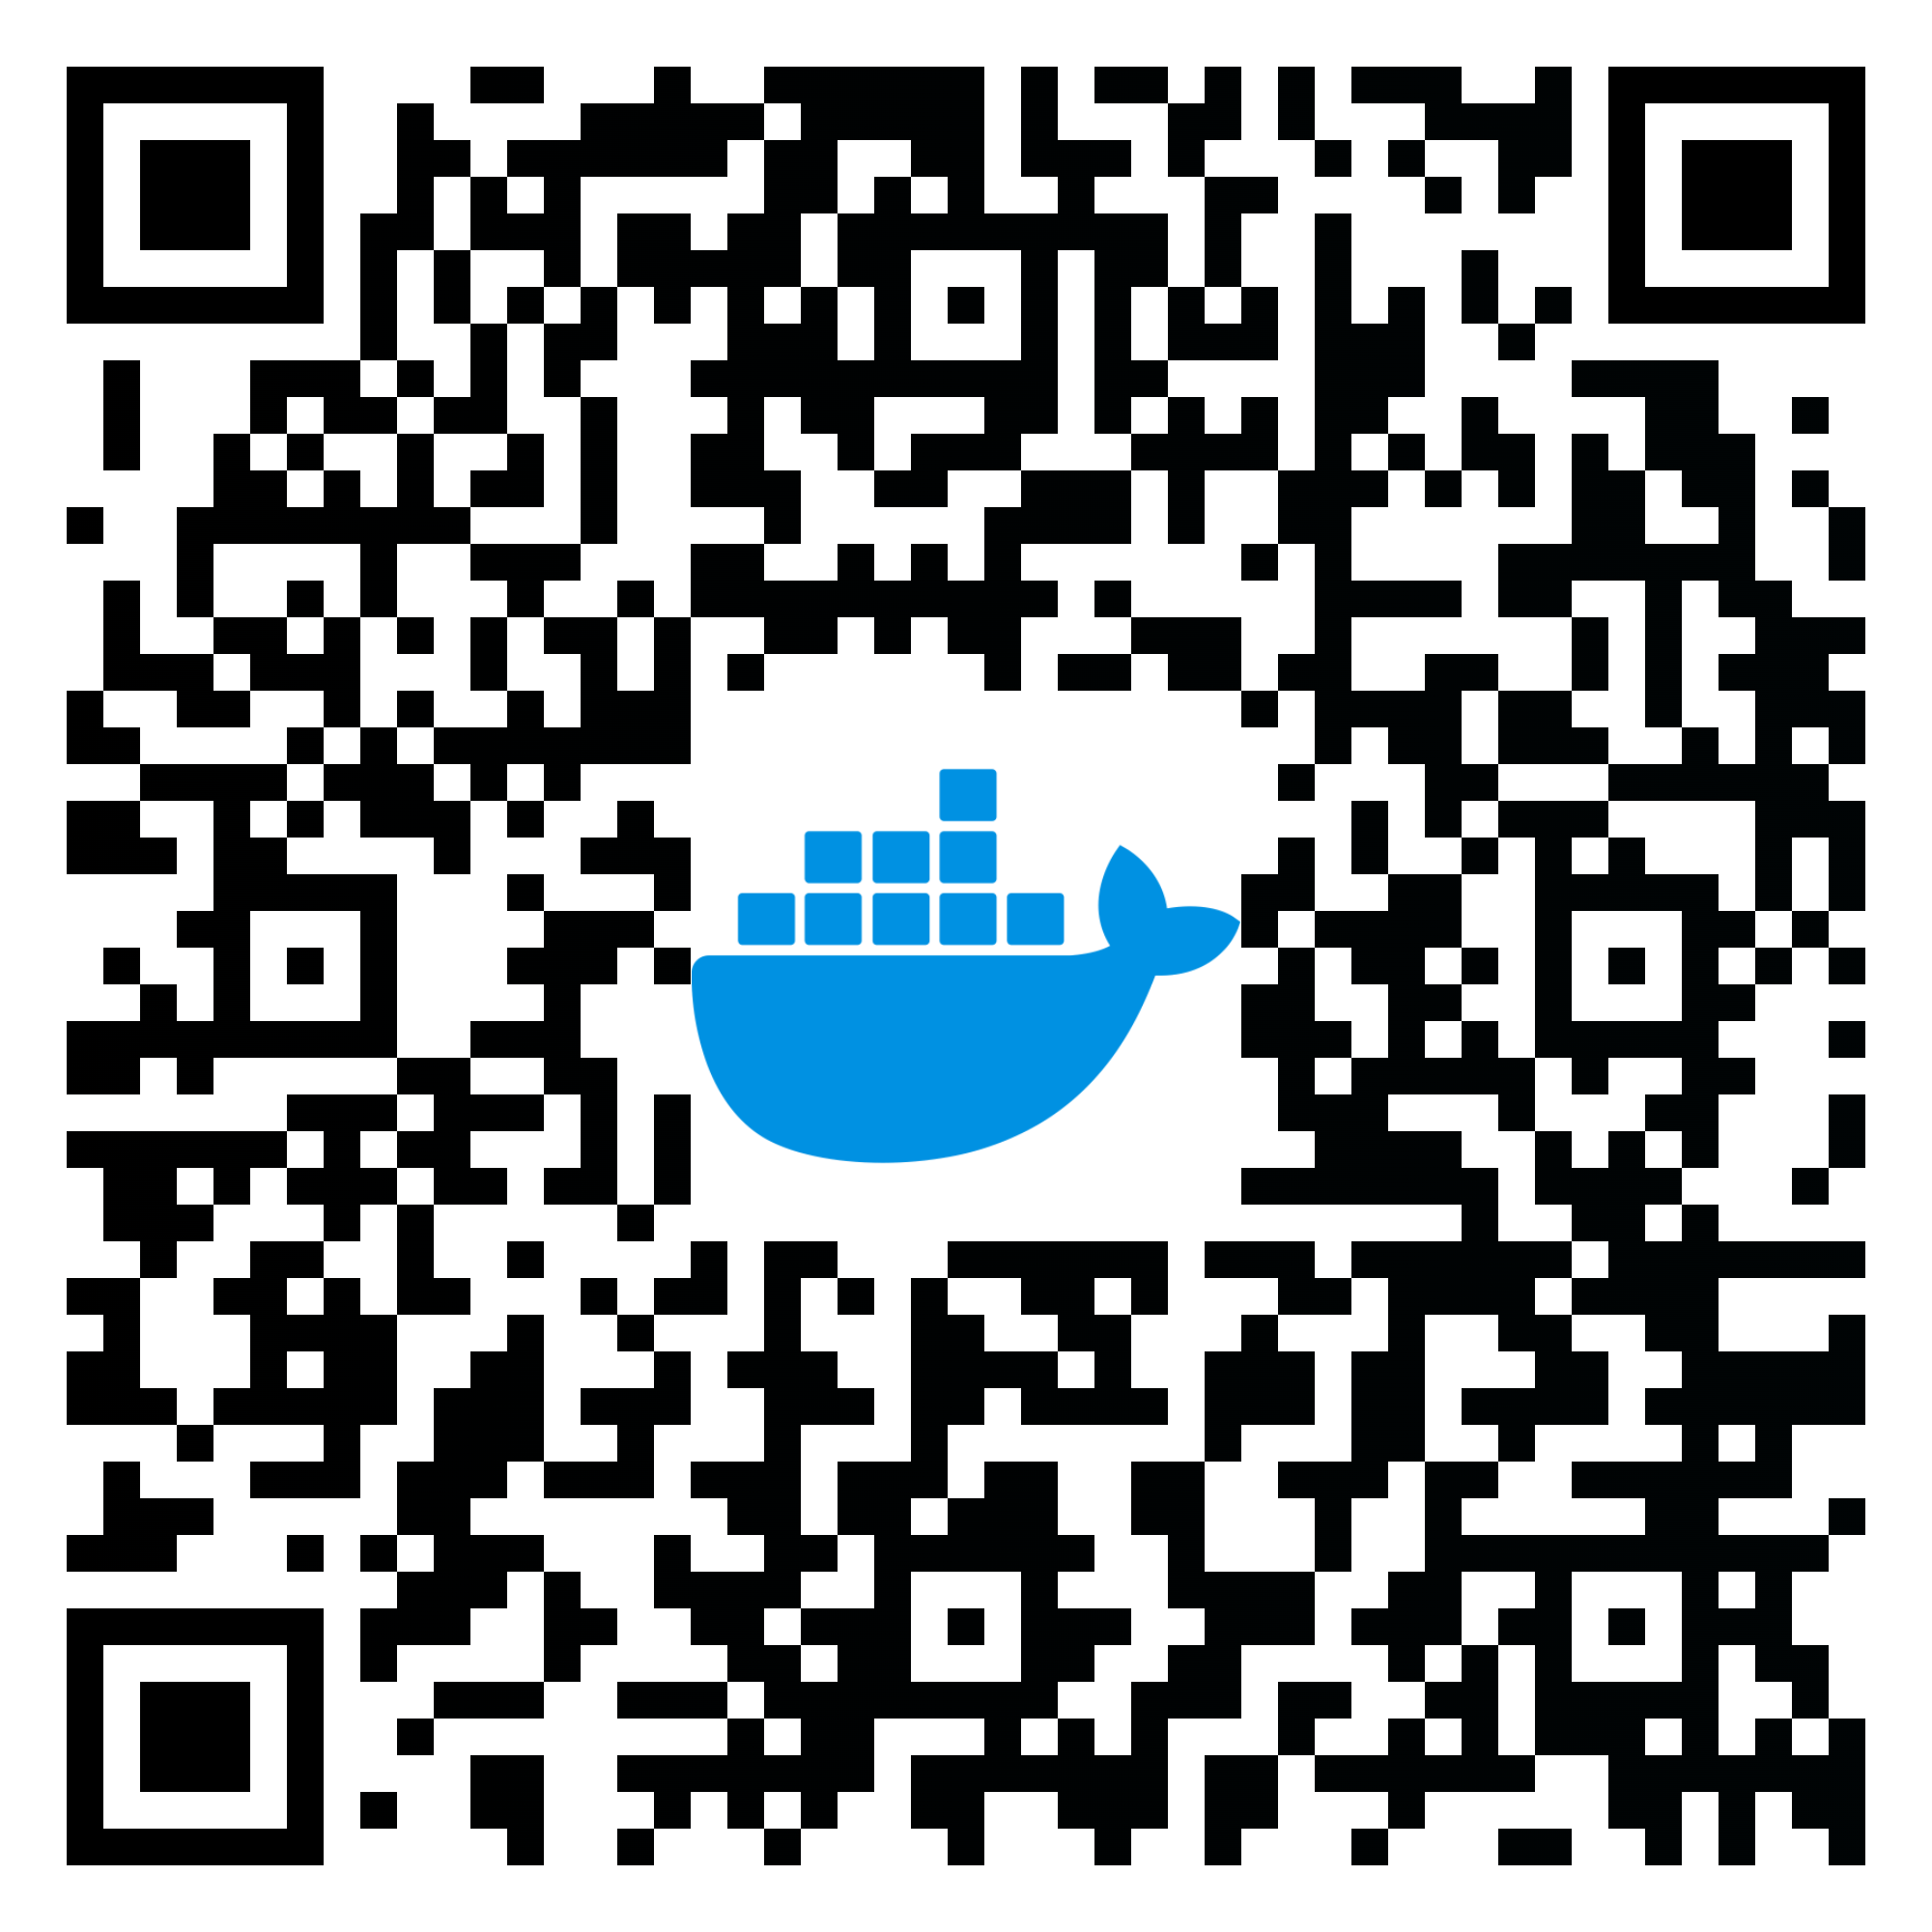
\includegraphics[width=1.2in]{figures/qr-code-dockerhub.png} 
        \captionsetup{justification=centering, singlelinecheck=false, labelsep=space}
        \caption{\href{https://hub.docker.com/repository/docker/werrnnnwerrrnnnnnn/match_web/general}{Dockerhub Repository: AIT Match}}
        \label{fig:dockerhub_qr}
        \end{figure}

    \newpage
    \section{User Interface Results}
    
        \subsection{Landing Page: Welcome}
        \begin{figure}[h]
                \centering
                \captionsetup{justification=centering, singlelinecheck=false, labelsep=space}
                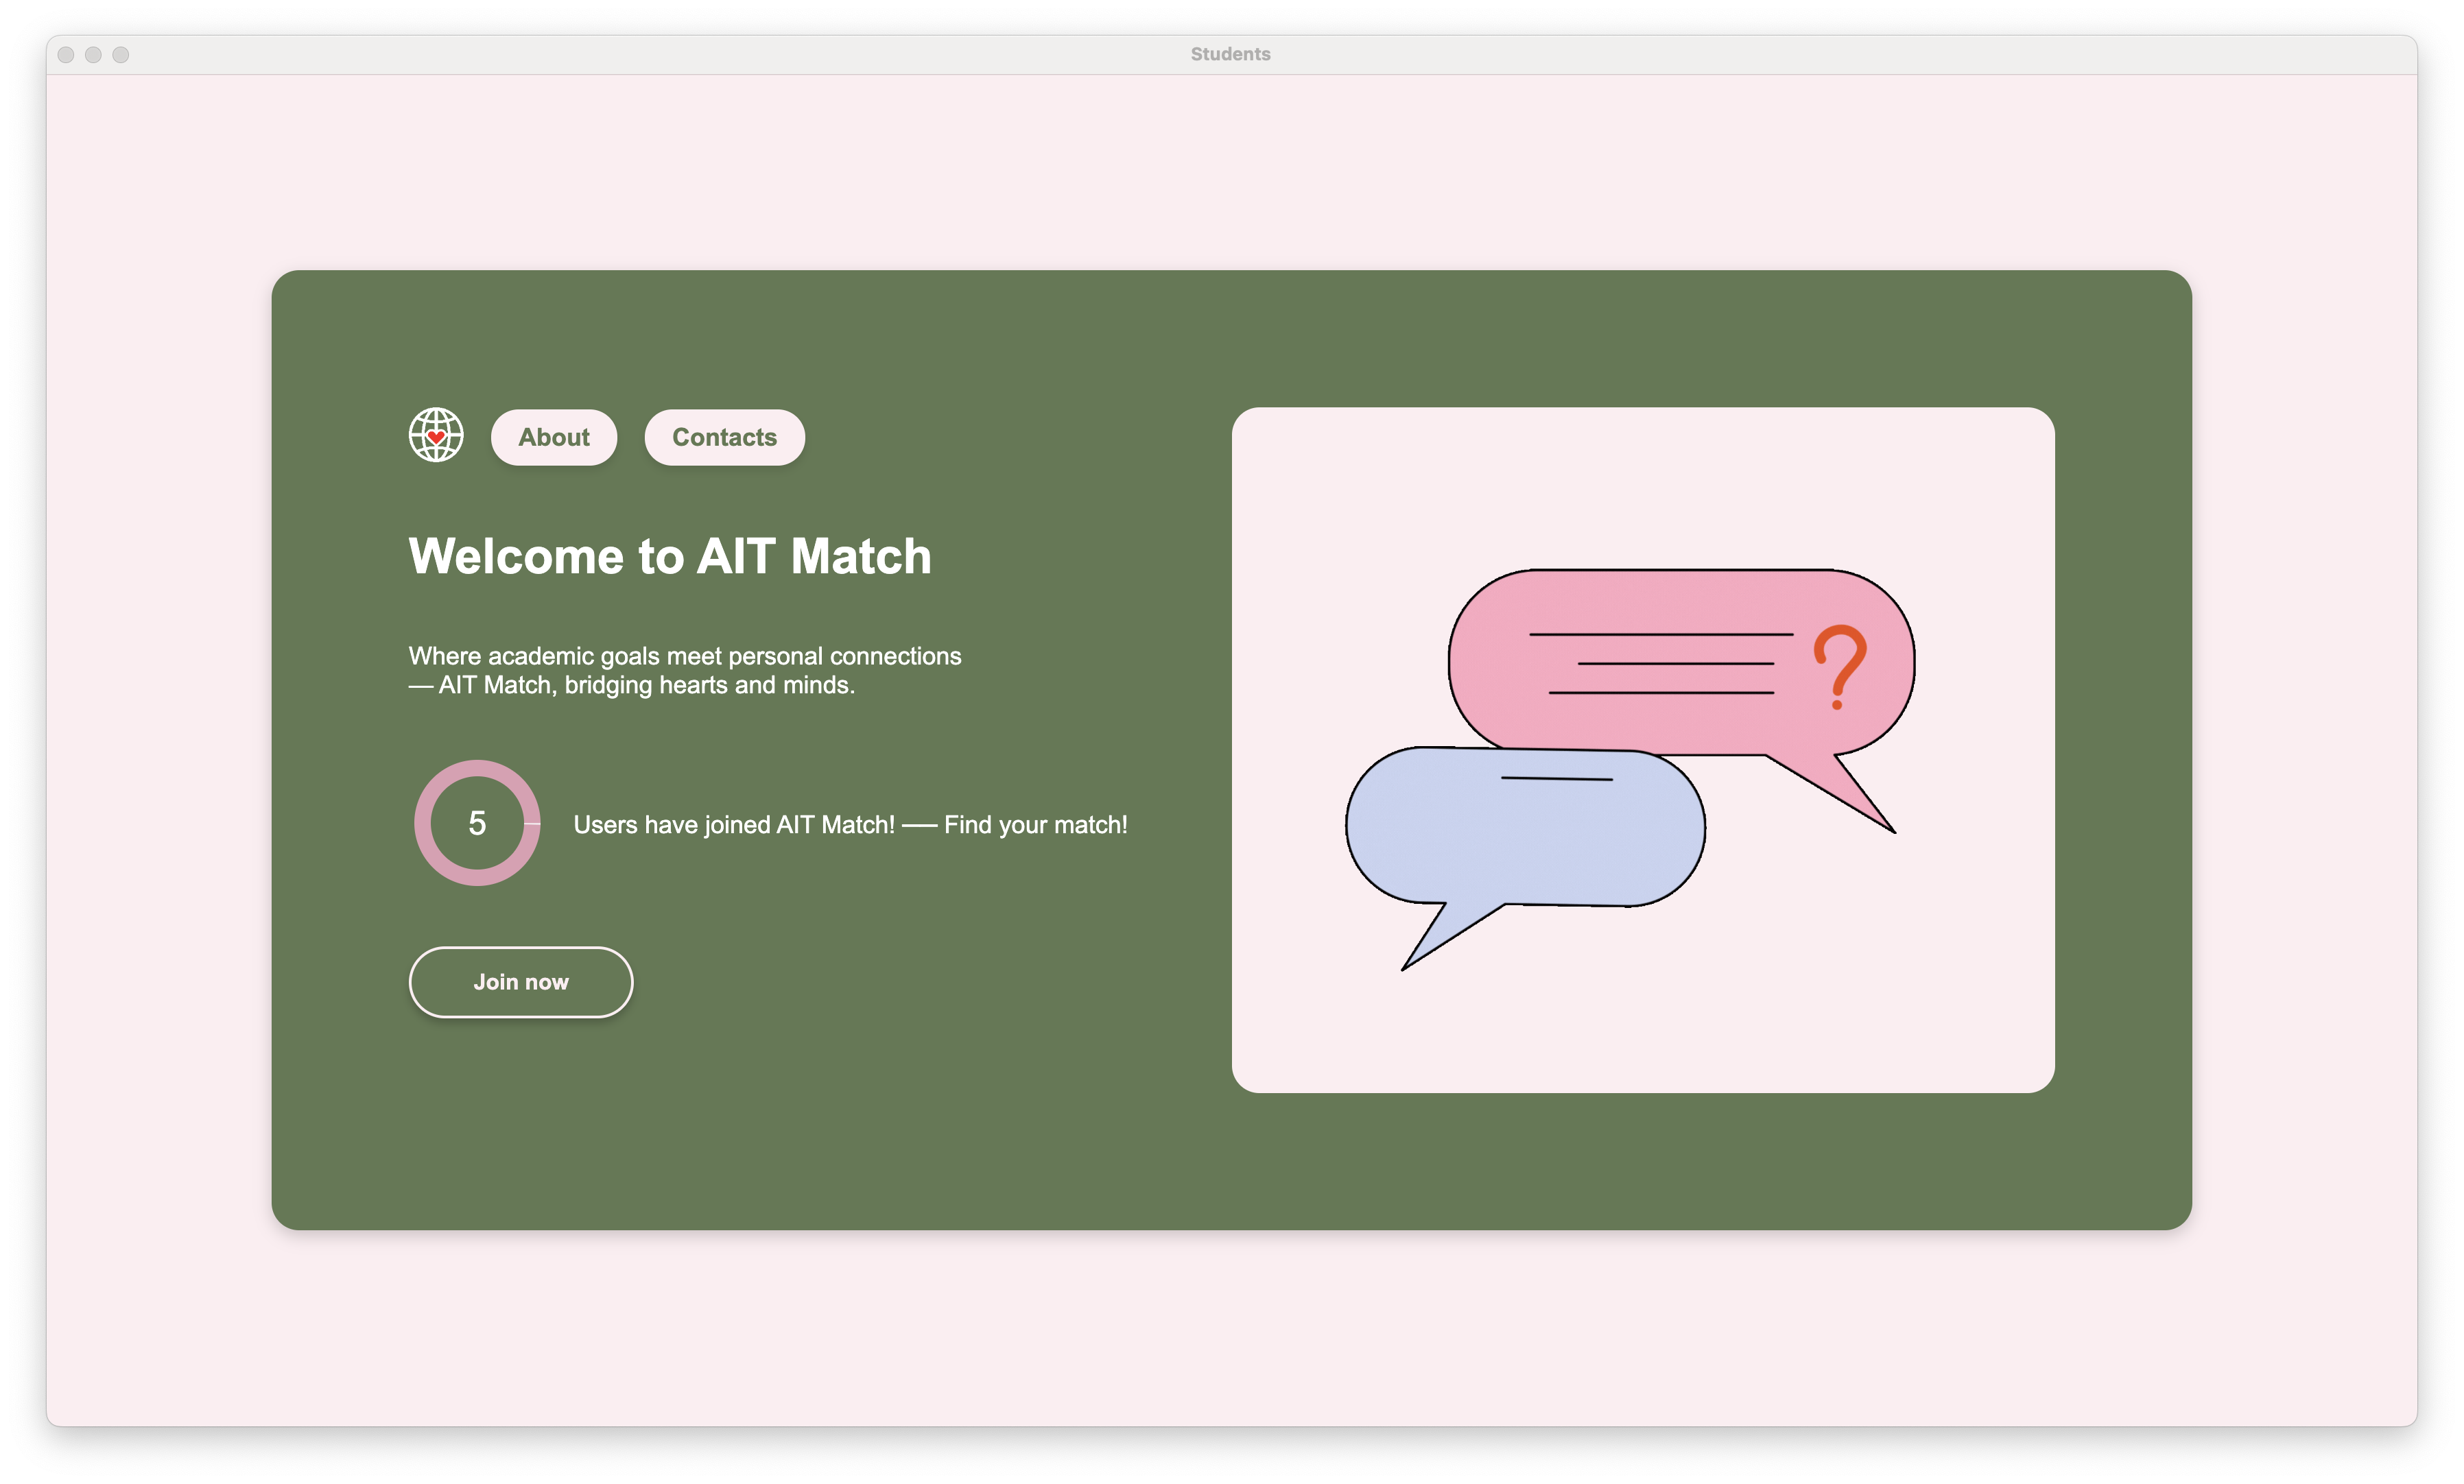
\includegraphics[width=5in]{figures/results/landing-page/welcome-page.png} 
                \caption{Welcome Page.}
                \label{fig:welcome-page}
            \end{figure}  

        \subsection{Landing Page: About}
        \begin{figure}[h]
                \centering
                \captionsetup{justification=centering, singlelinecheck=false, labelsep=space}
                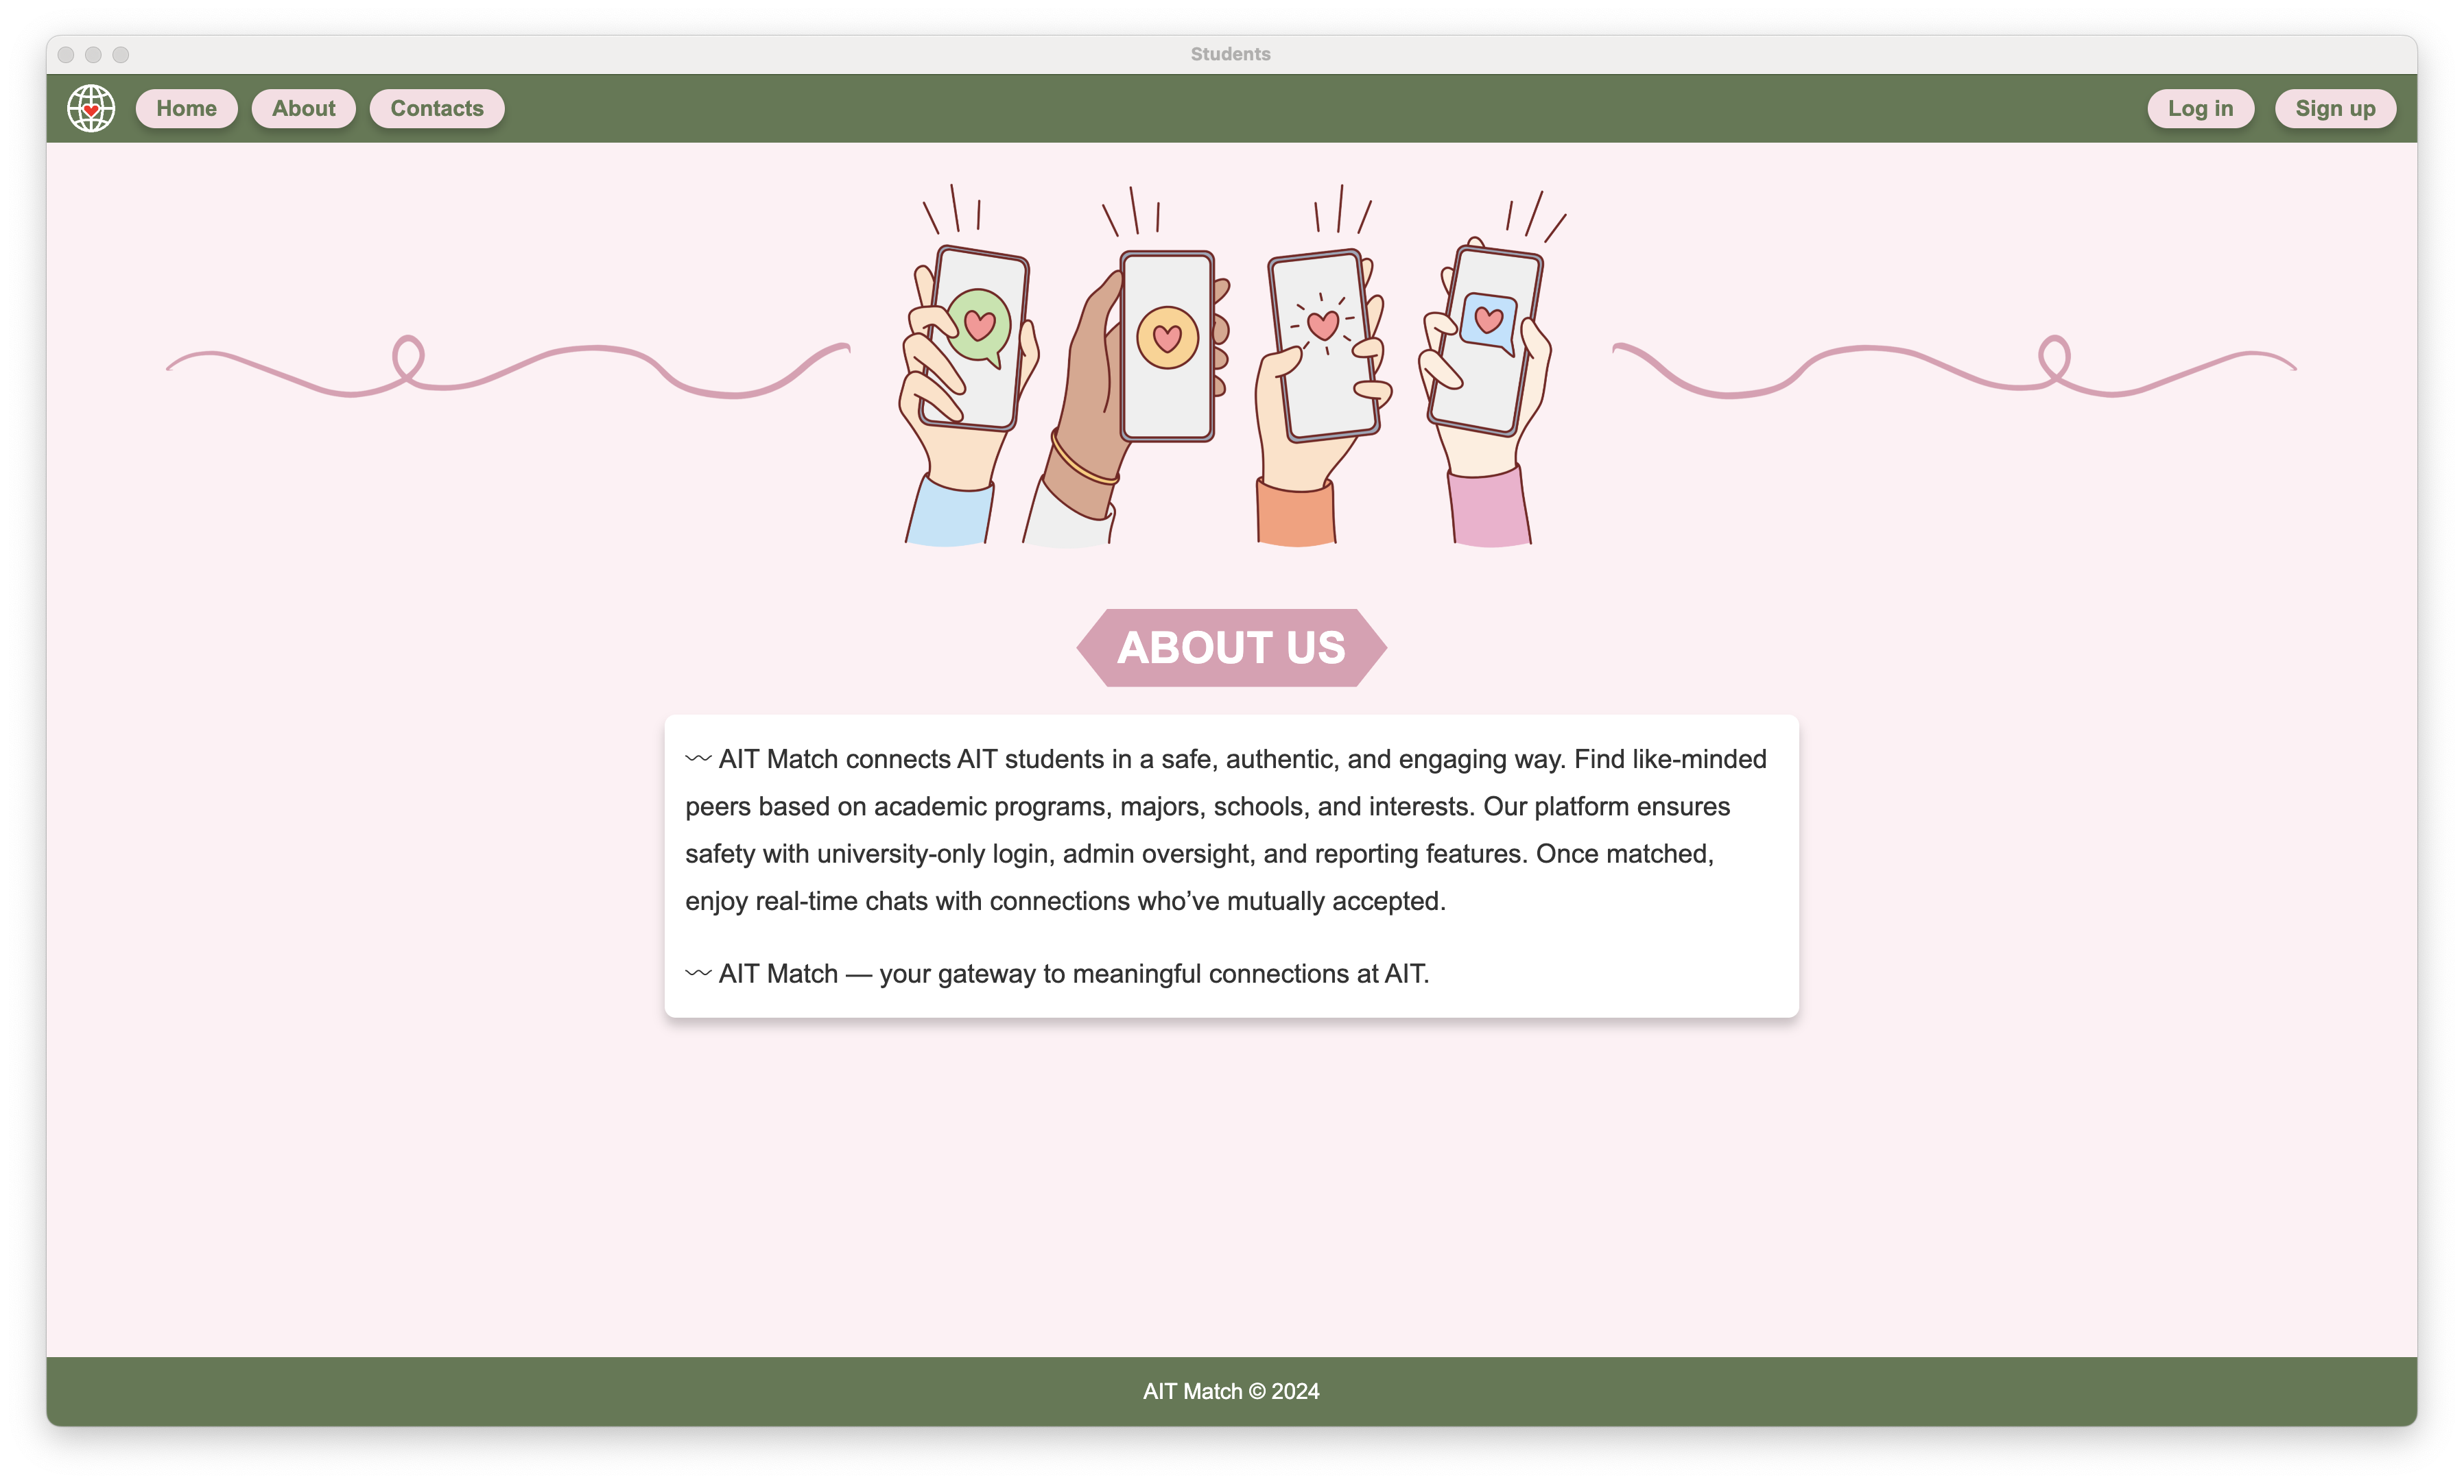
\includegraphics[width=5in]{figures/results/landing-page/about-page.png} 
                \caption{About Page.}
                \label{fig:about-page}
            \end{figure}  

        \newpage
        \subsection{Landing Page: Contact}
        \begin{figure}[h]
                \centering
                \captionsetup{justification=centering, singlelinecheck=false, labelsep=space}
                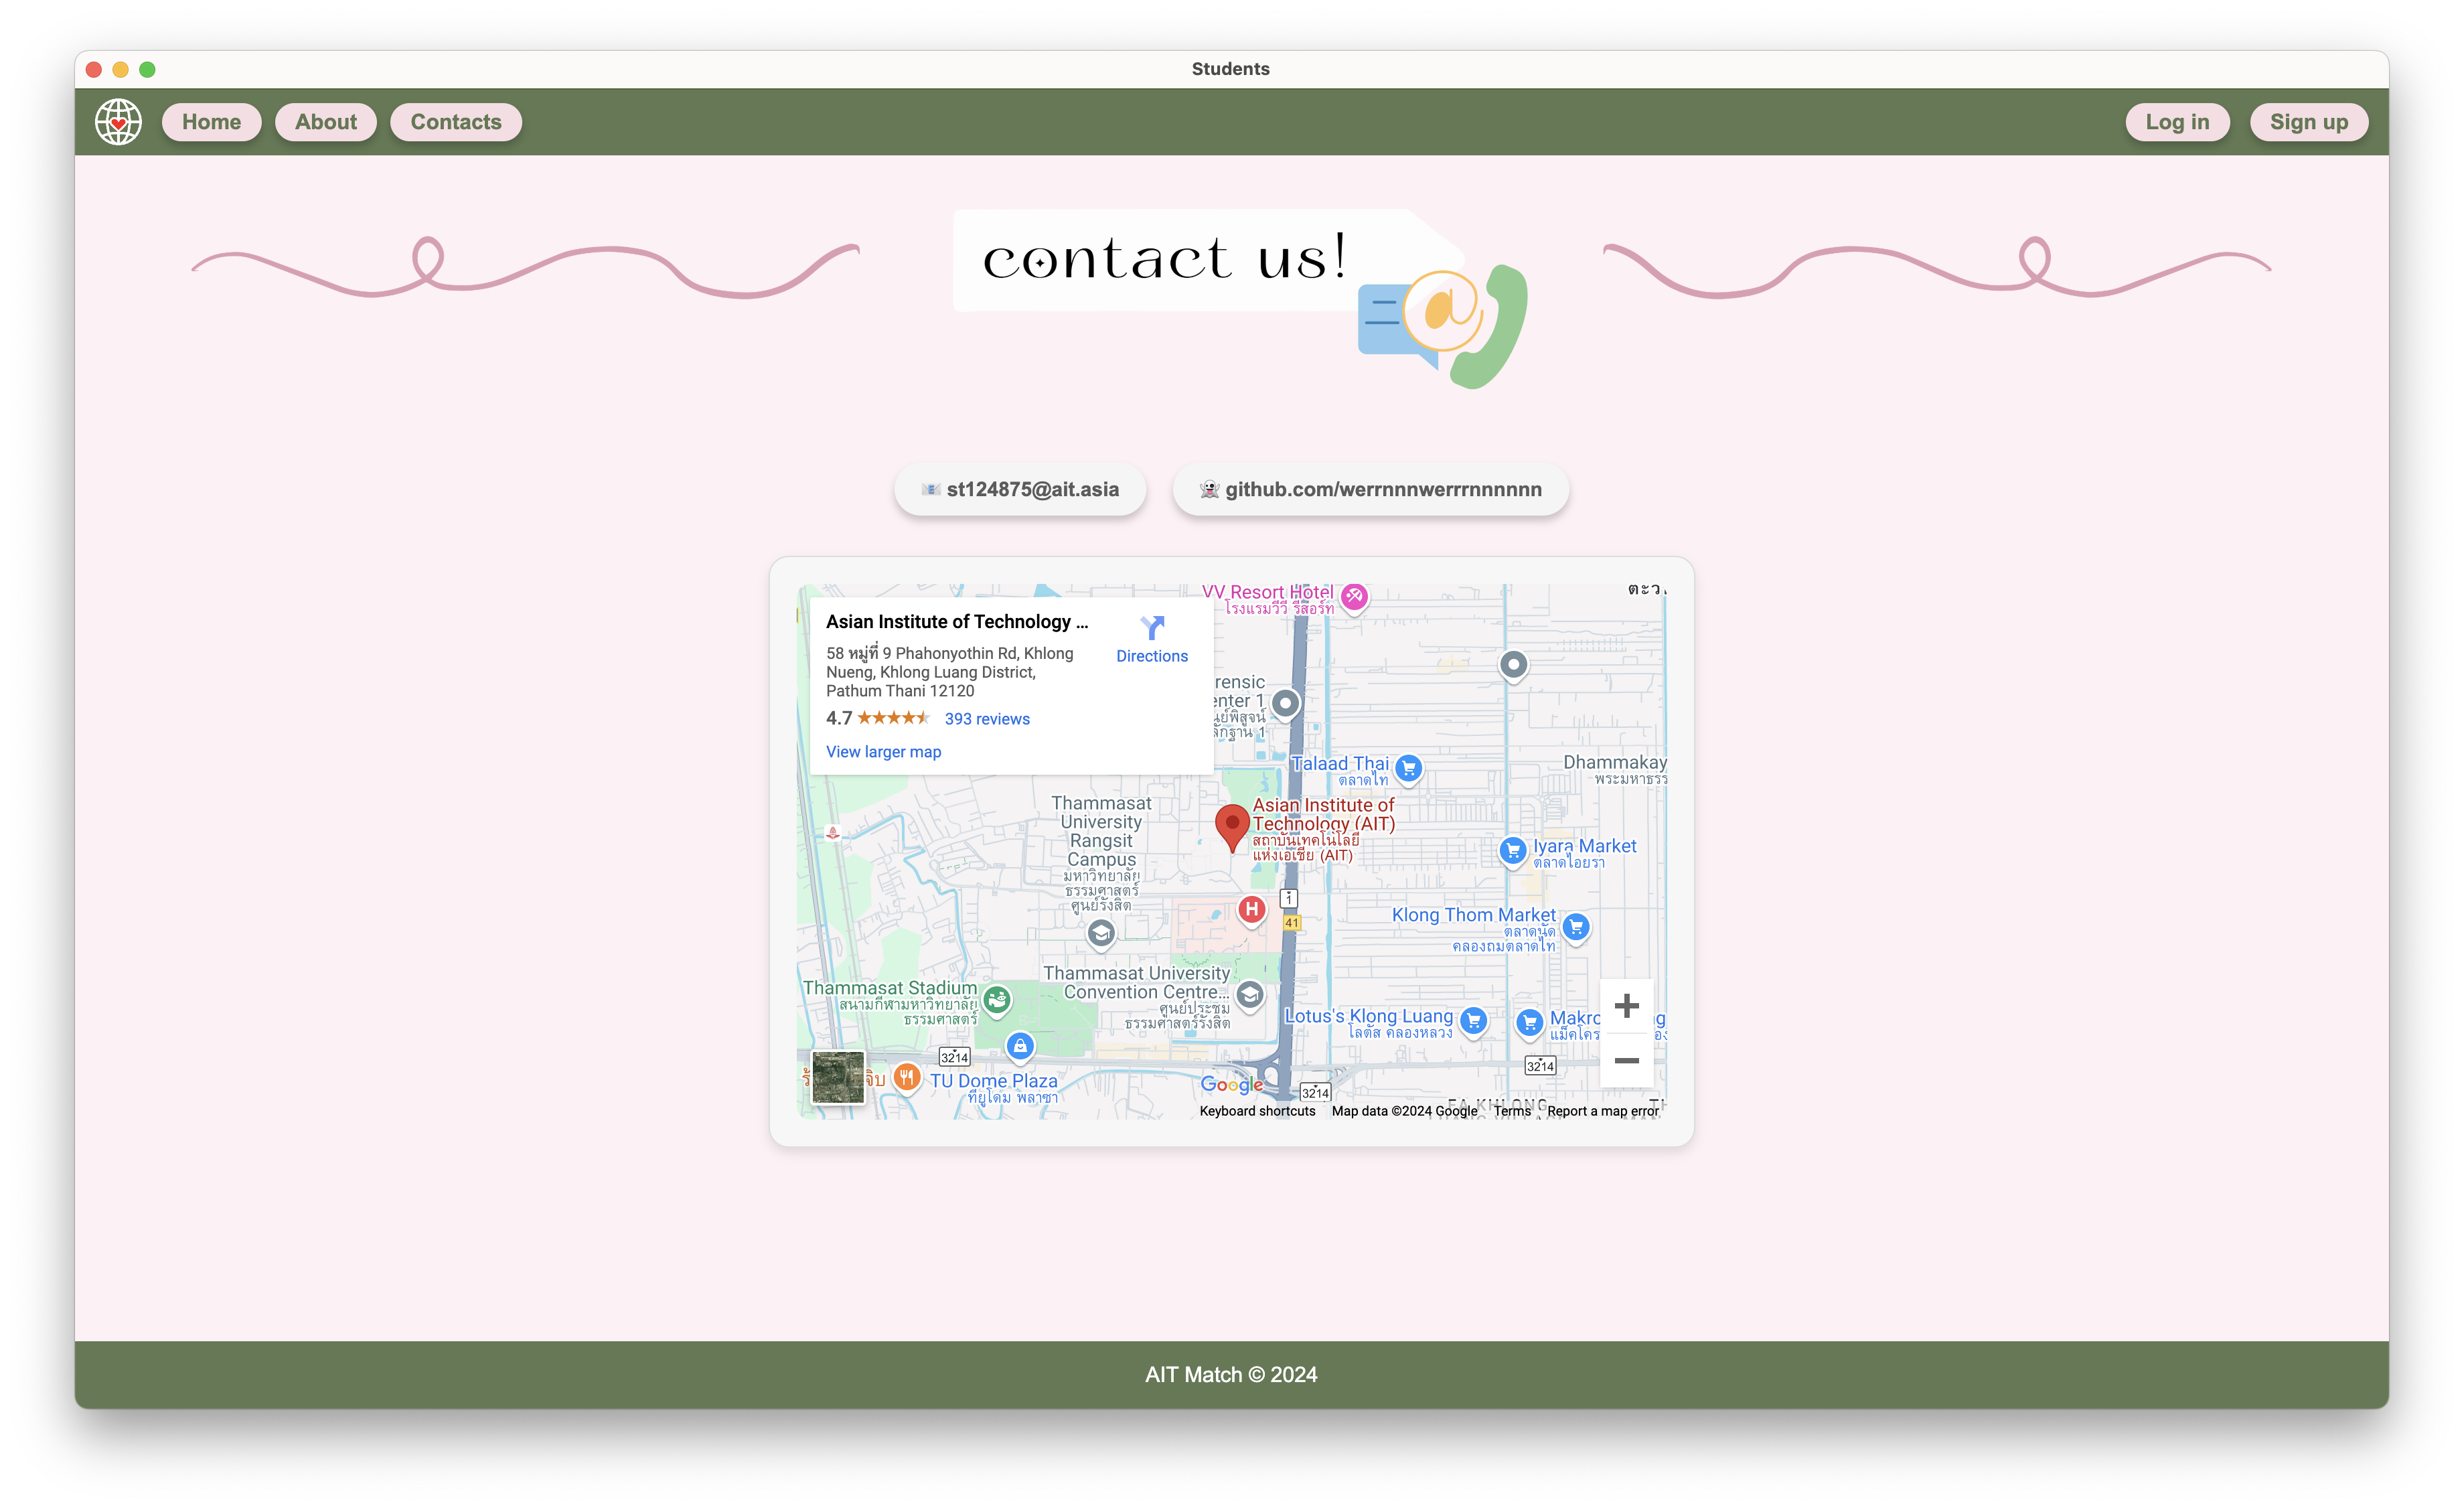
\includegraphics[width=5in]{figures/results/landing-page/contact-page.png} 
                \caption{Contact Page.}
                \label{fig:contact-page}
            \end{figure}  
% ------------------------------------------------- %
        \newpage
        \subsection{User Authentication: Sign Up Page}
        \begin{figure}[h]
                \centering
                \captionsetup{justification=centering, singlelinecheck=false, labelsep=space}
                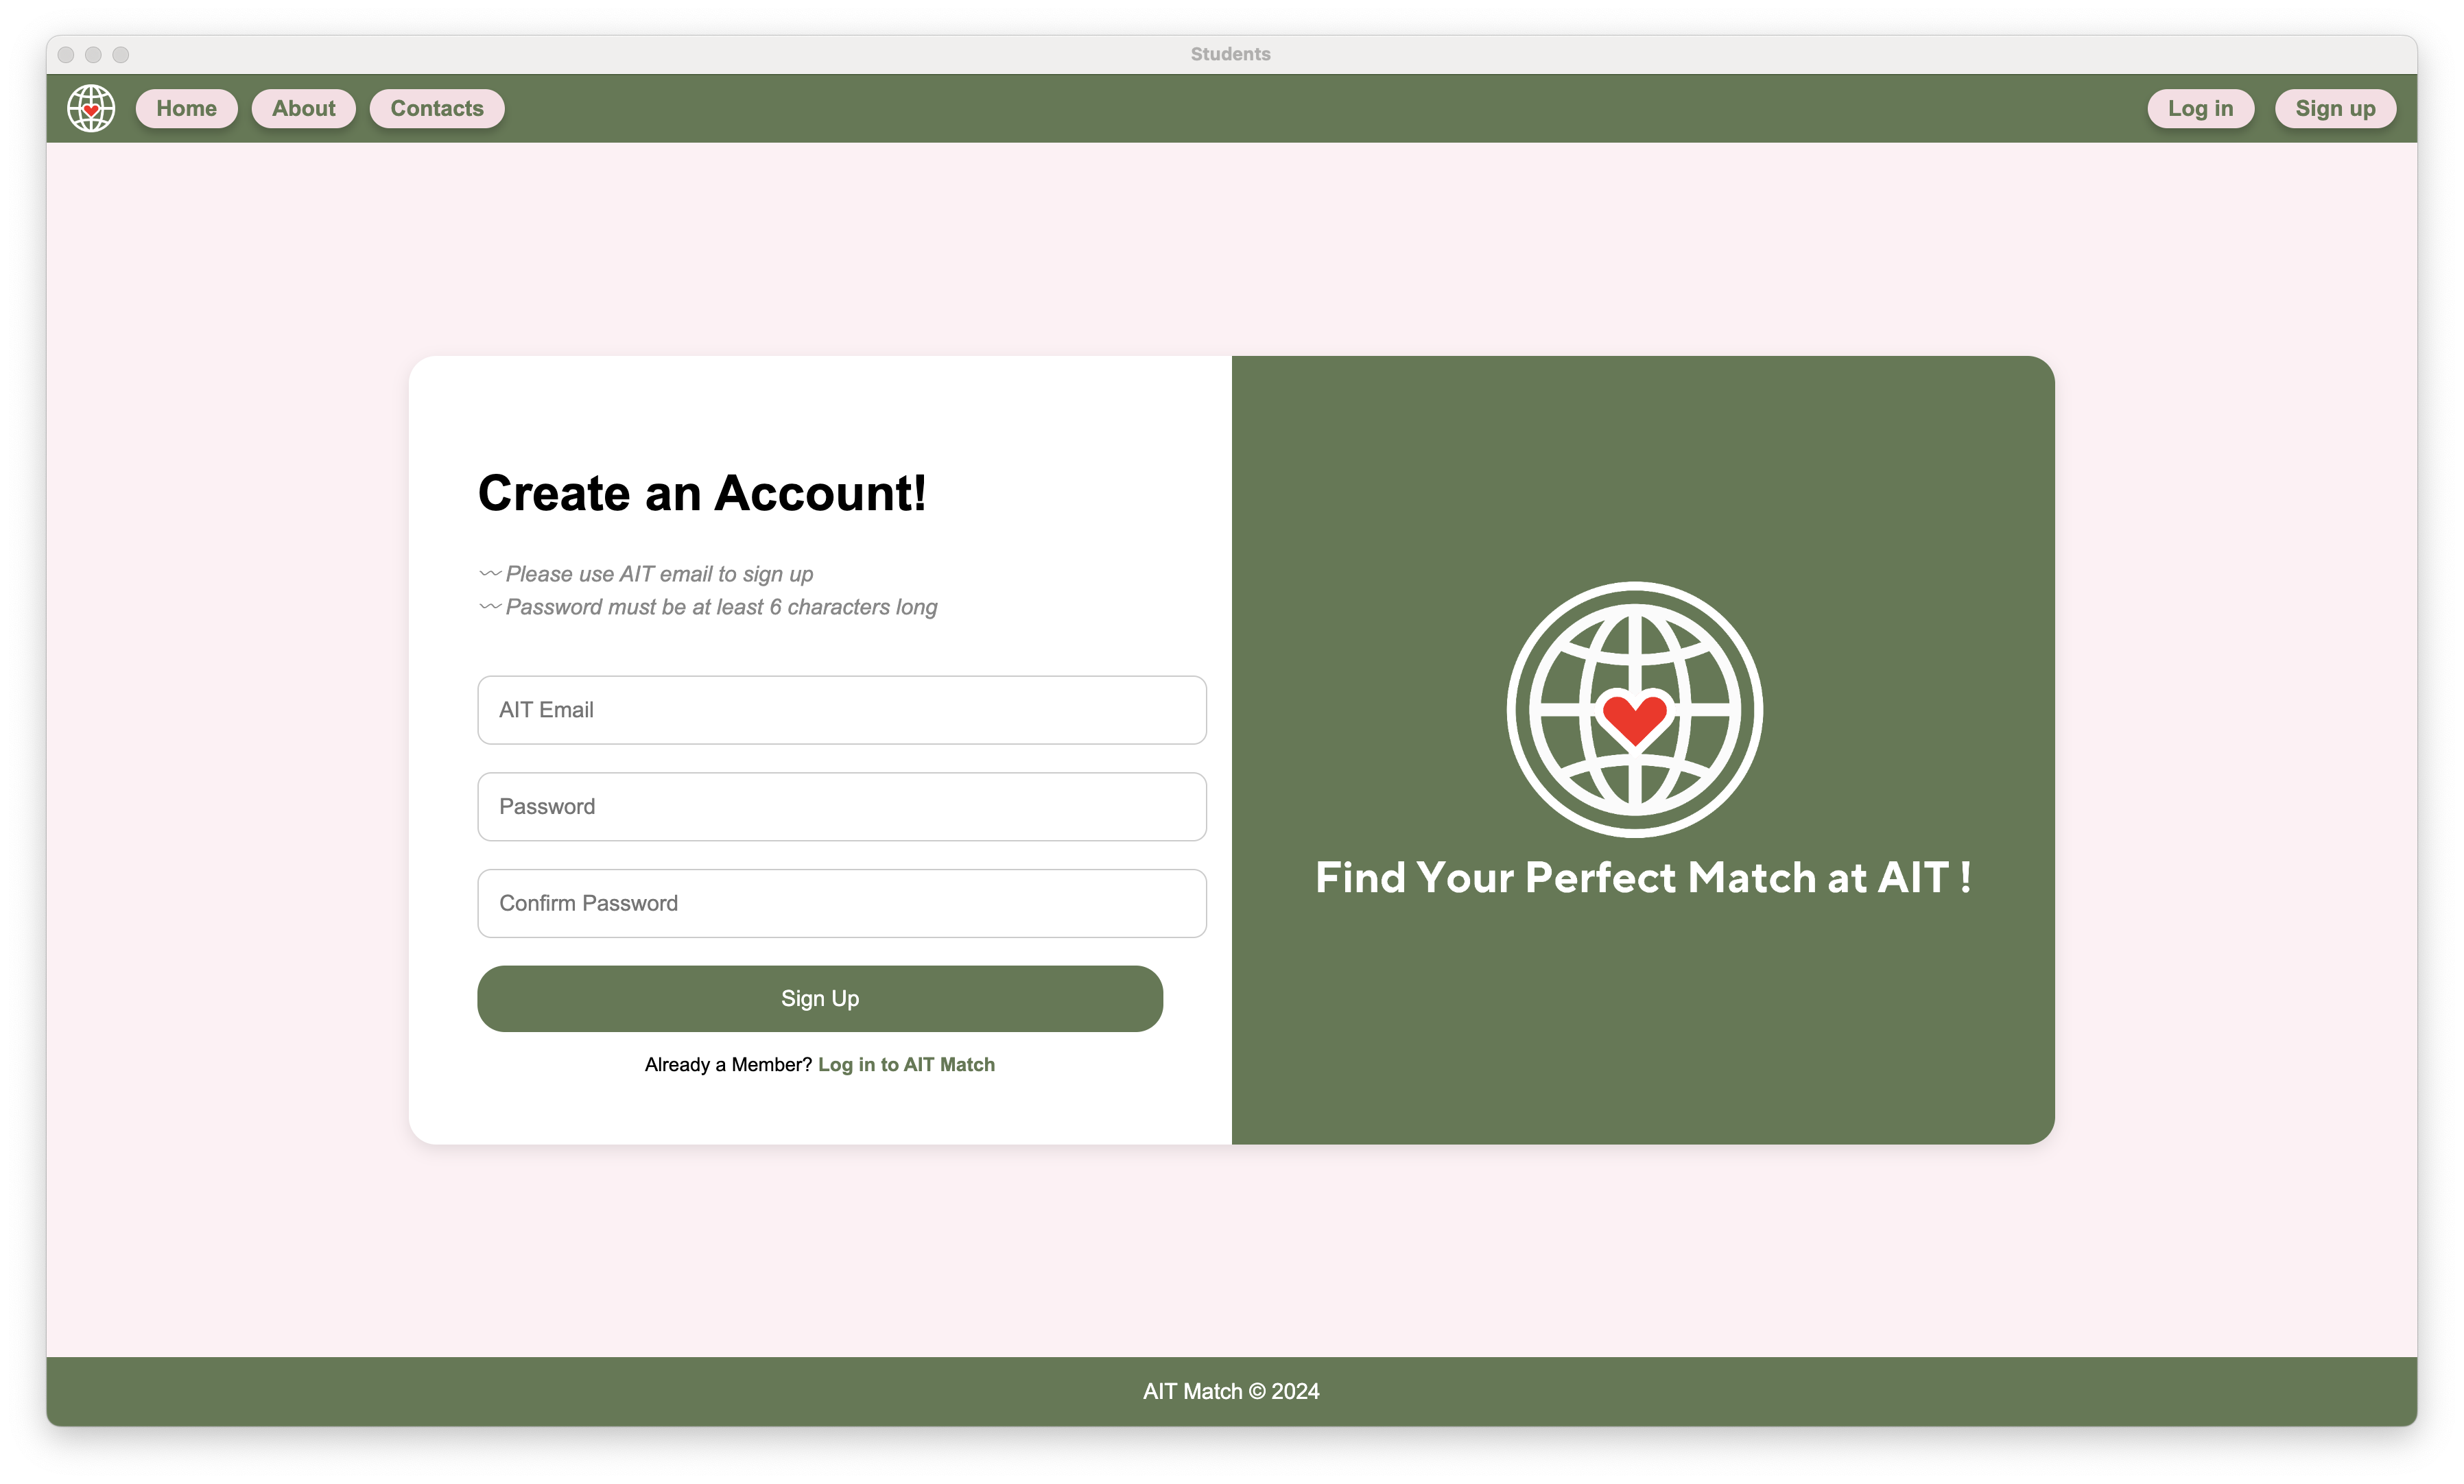
\includegraphics[width=5in]{figures/results/landing-page/signup-page.png} 
                \caption{Sign Up Page.}
                \label{fig:signup-page}
            \end{figure}

        \subsection{User Authentication Page: Login Page}
        \begin{figure}[h]
                \centering
                \captionsetup{justification=centering, singlelinecheck=false, labelsep=space}
                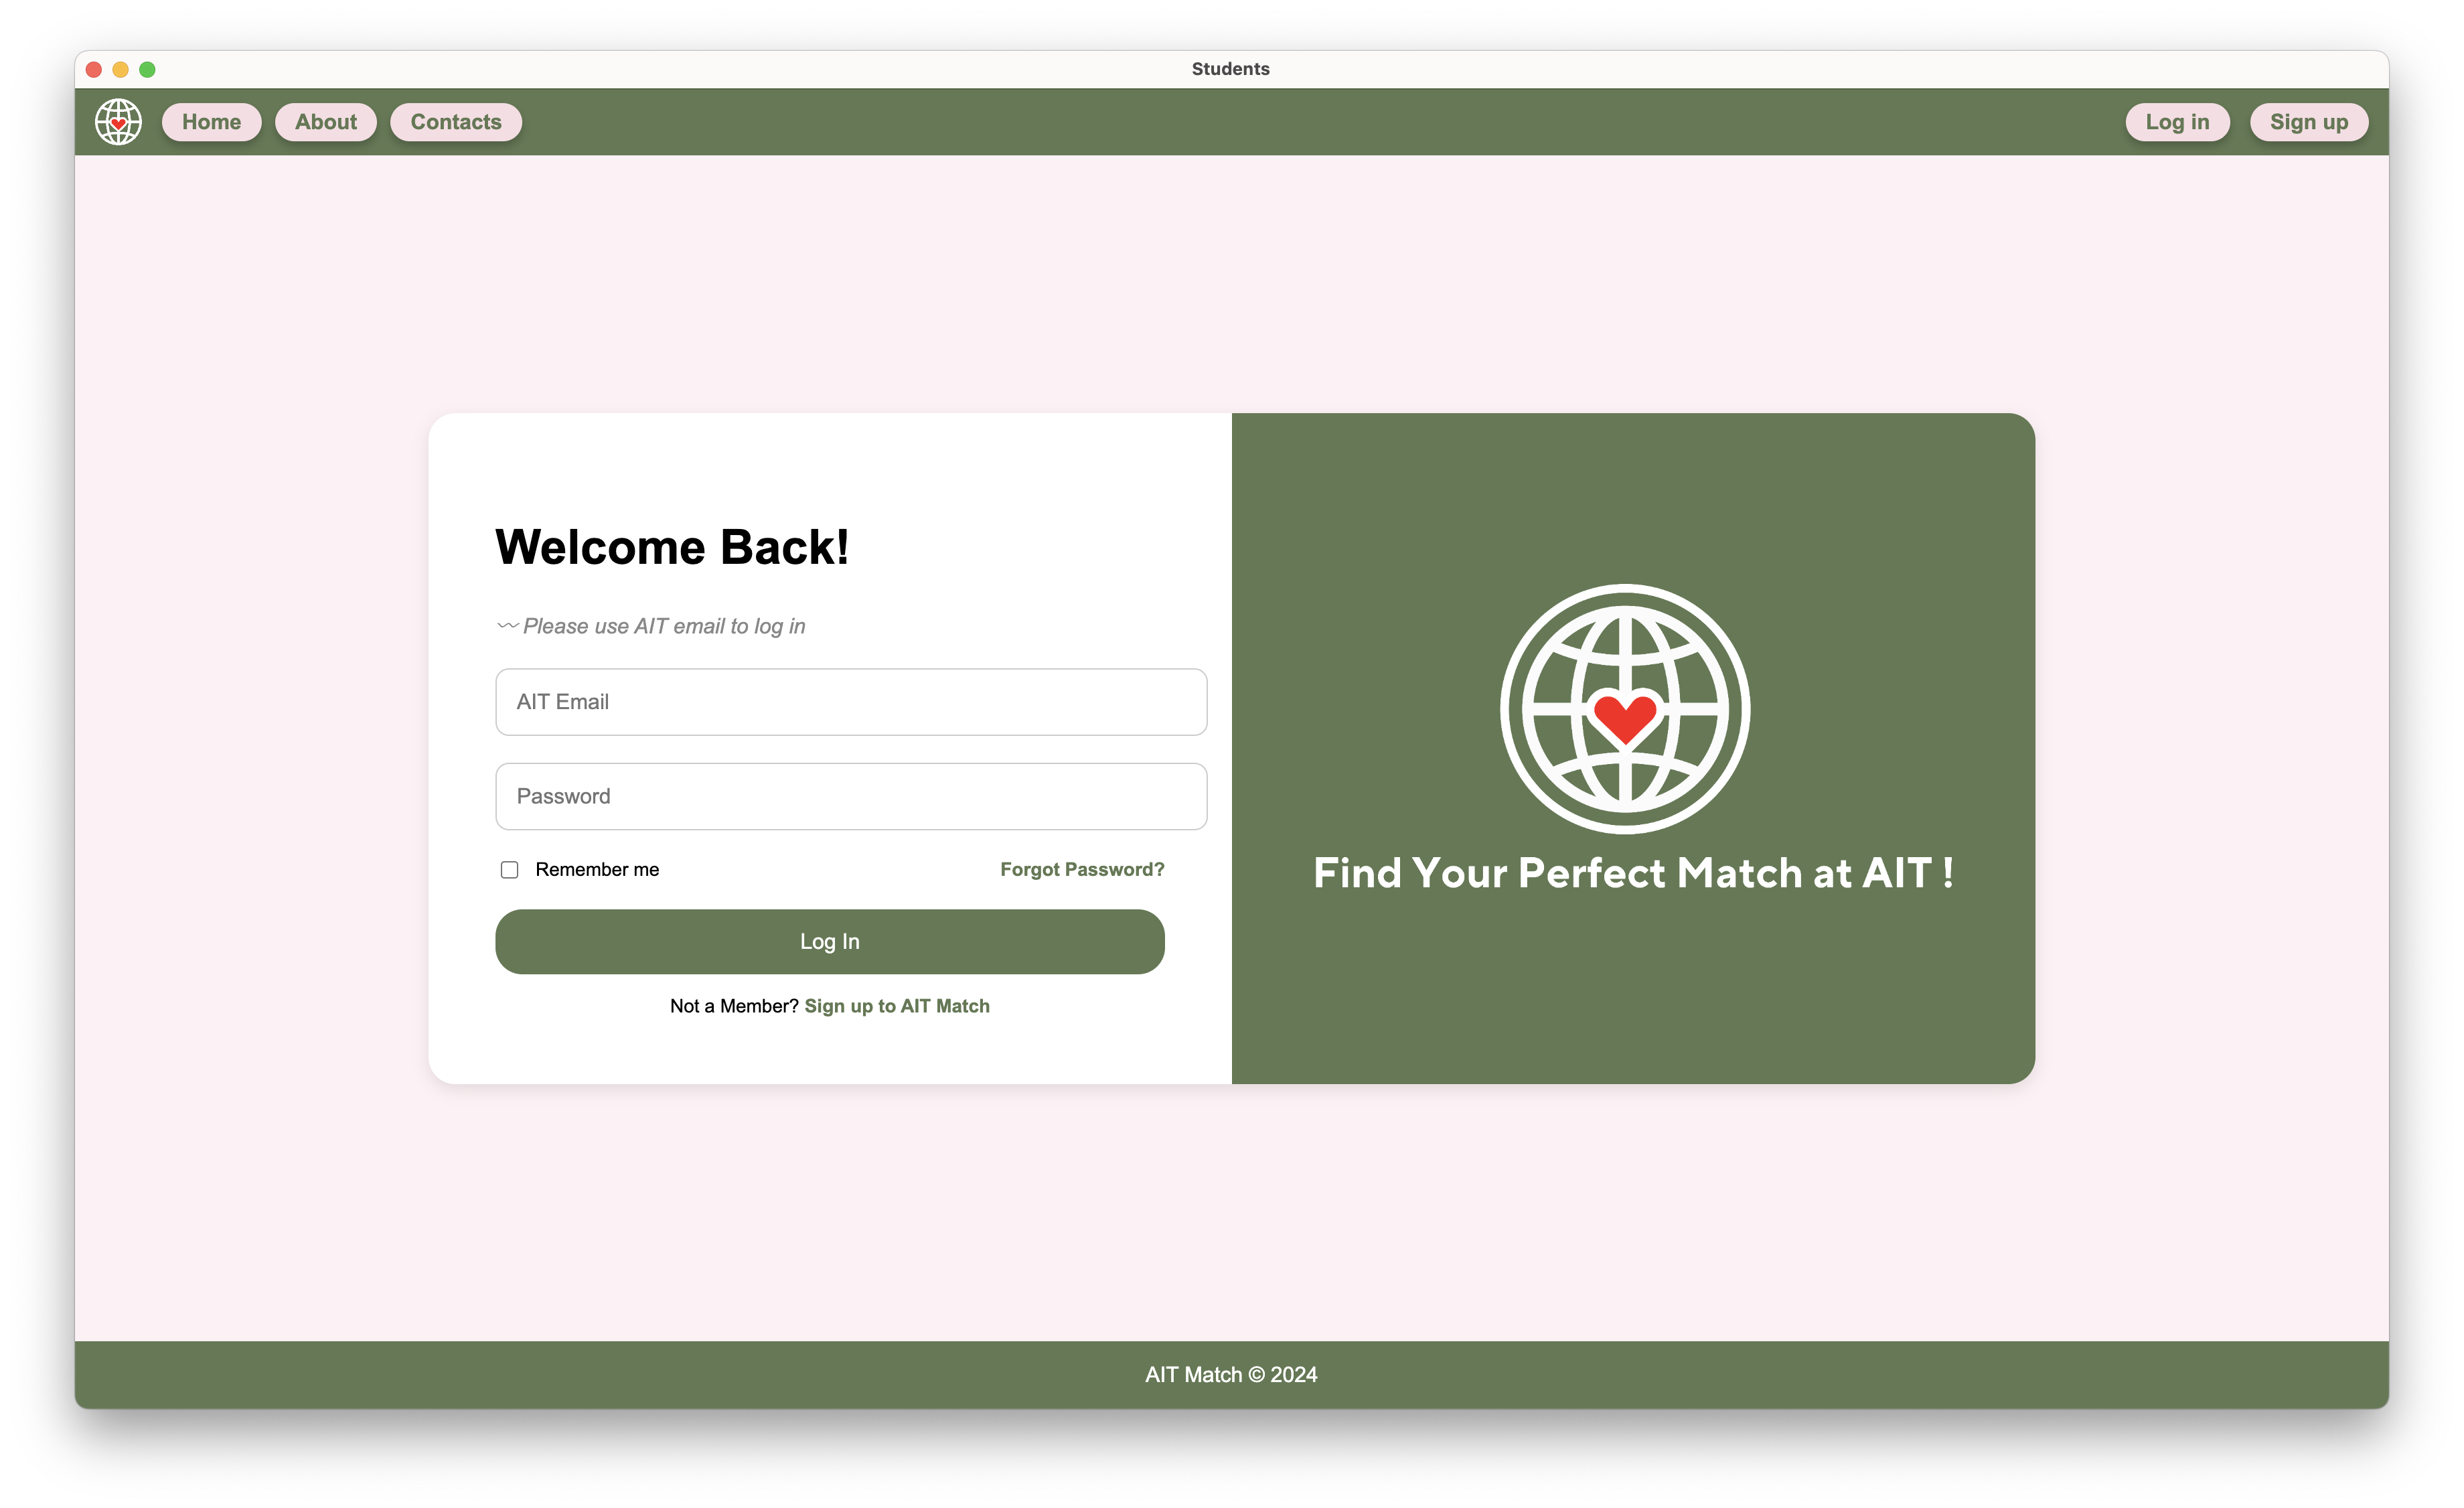
\includegraphics[width=5in]{figures/results/landing-page/login-page.png} 
                \caption{Login Page.}
                \label{fig:login-page}
            \end{figure}
% ------------------------------------------------- %
        \newpage
        \subsection{Profile: Profile Creation Page}
        \begin{figure}[h]
                \centering
                \captionsetup{justification=centering, singlelinecheck=false, labelsep=space}
                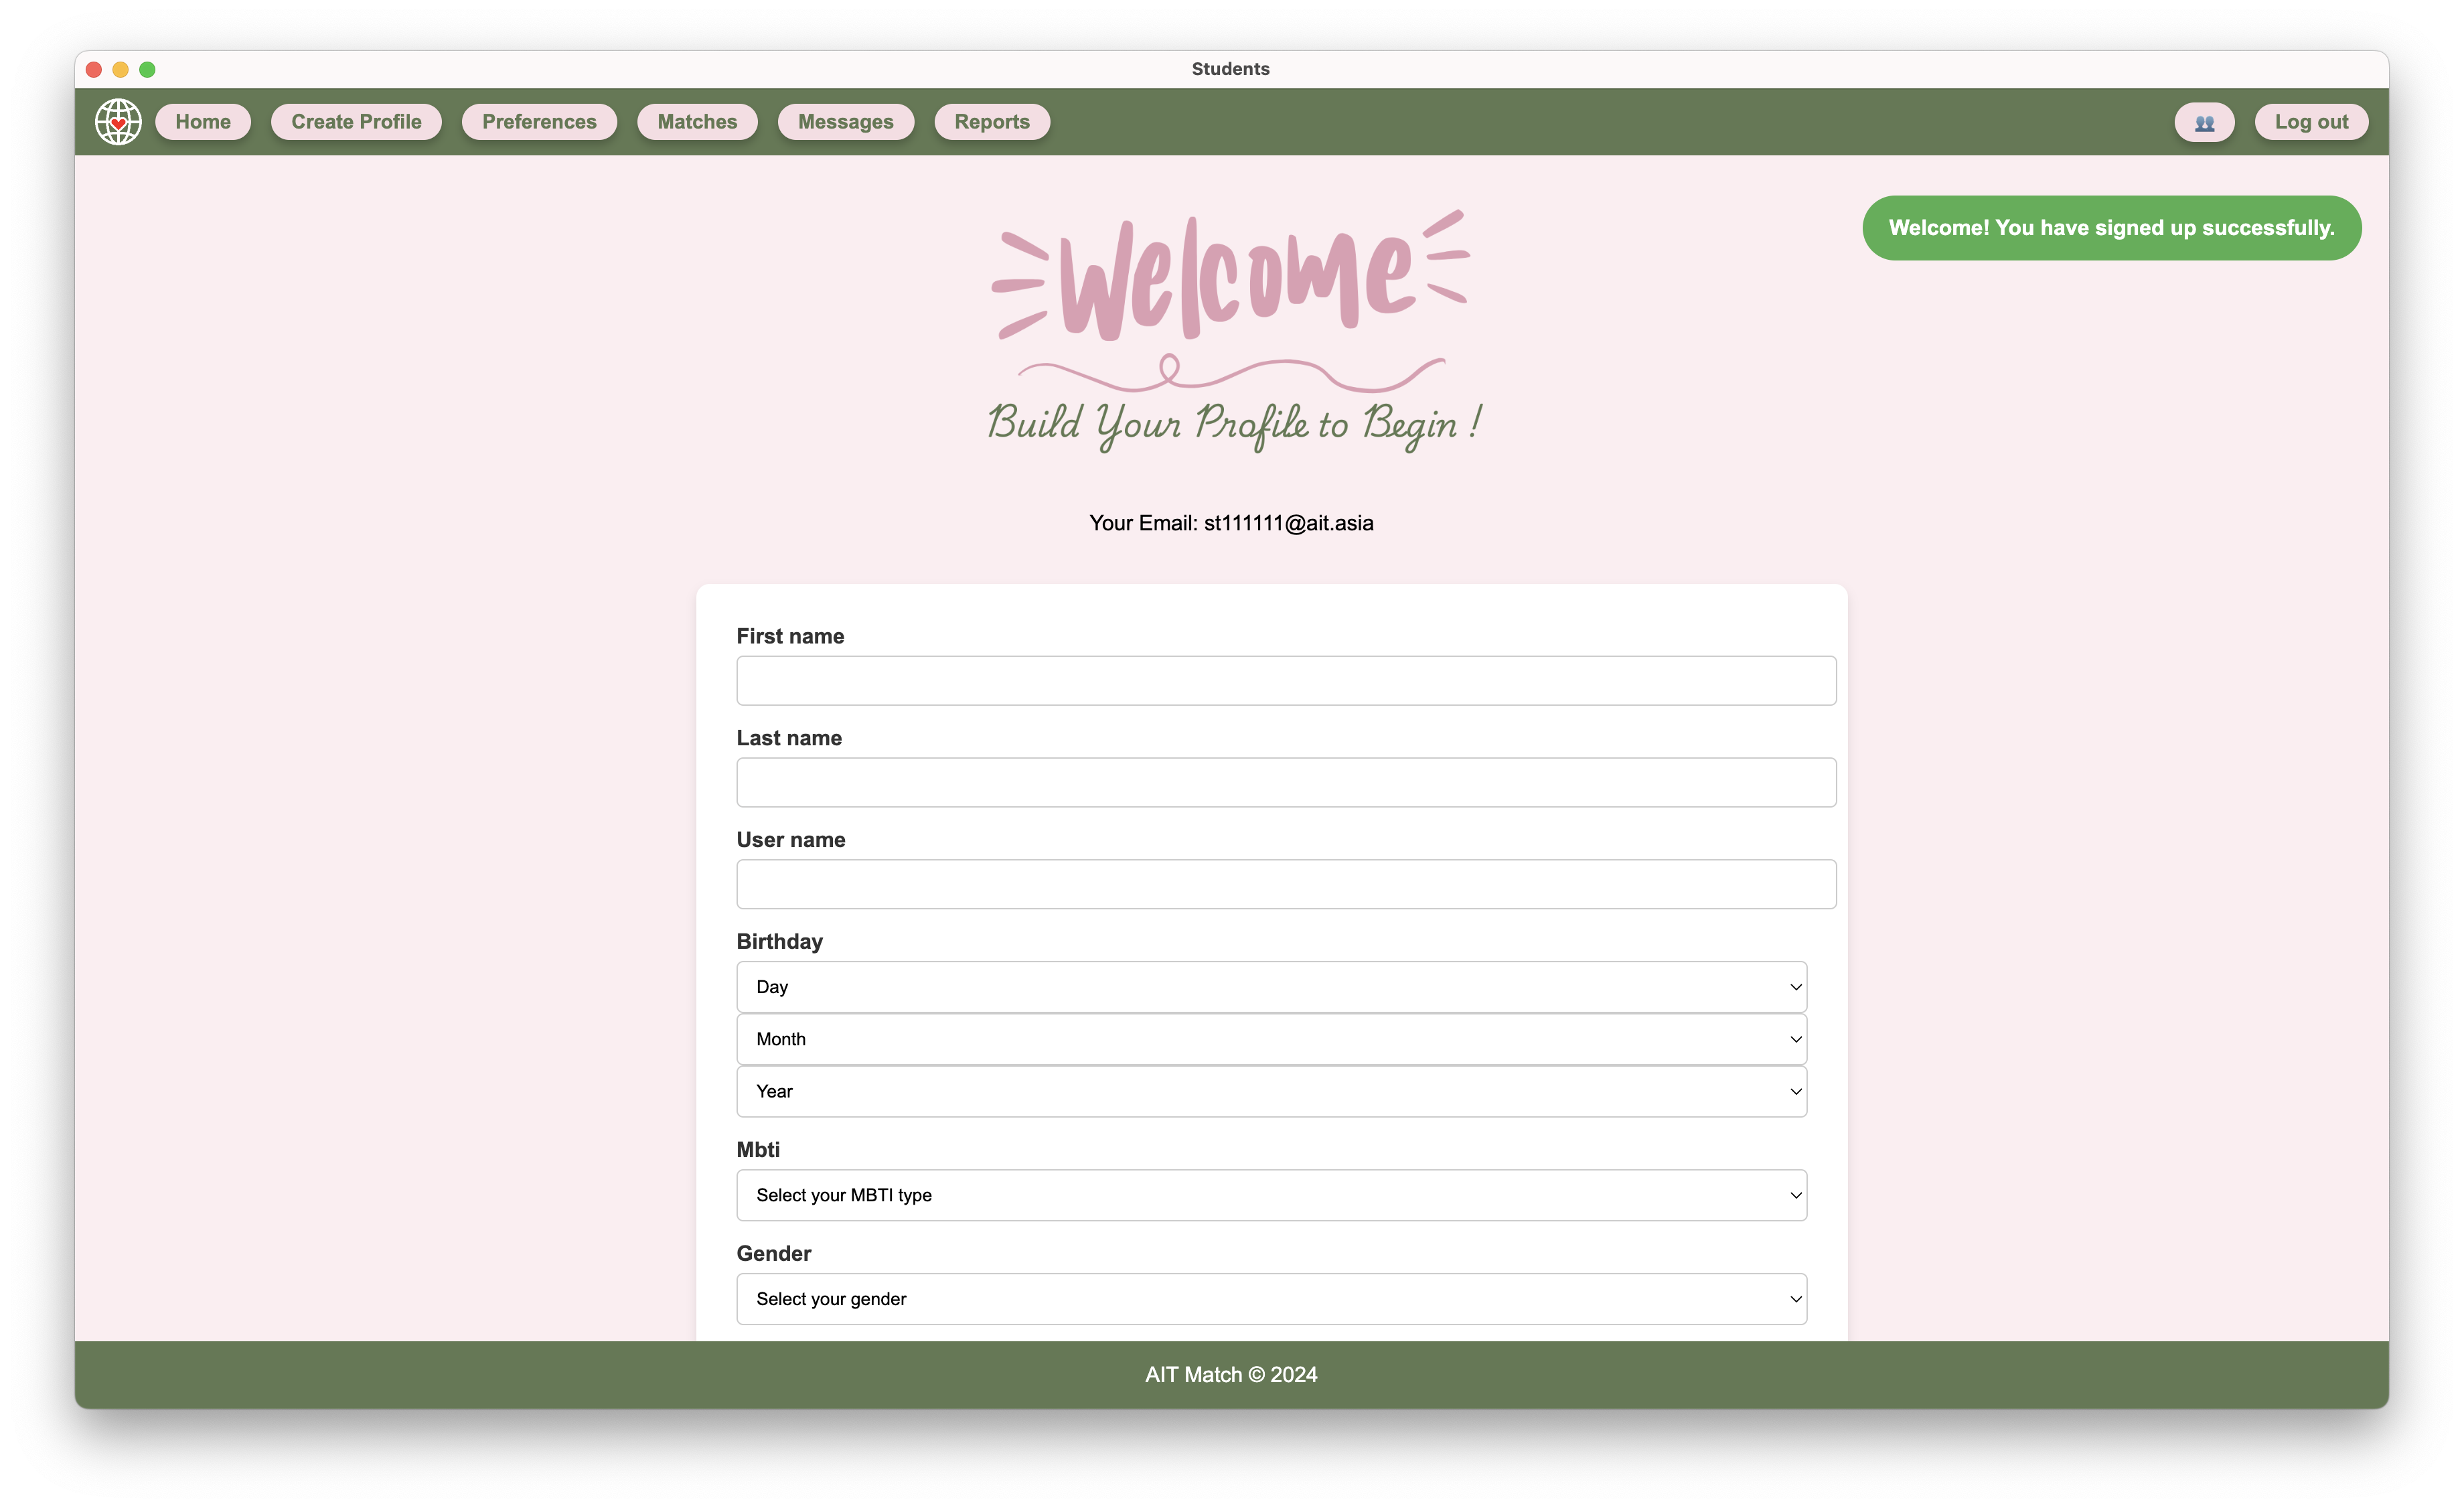
\includegraphics[width=5in]{figures/results/profiles/create-profile-page.png} 
                \caption{Profile CreationPage.}
                \label{fig:create-profile-page}
            \end{figure}

        \subsection{Profile: Profile Creation Page (Continued)}
        \begin{figure}[h]
                \centering
                \captionsetup{justification=centering, singlelinecheck=false, labelsep=space}
                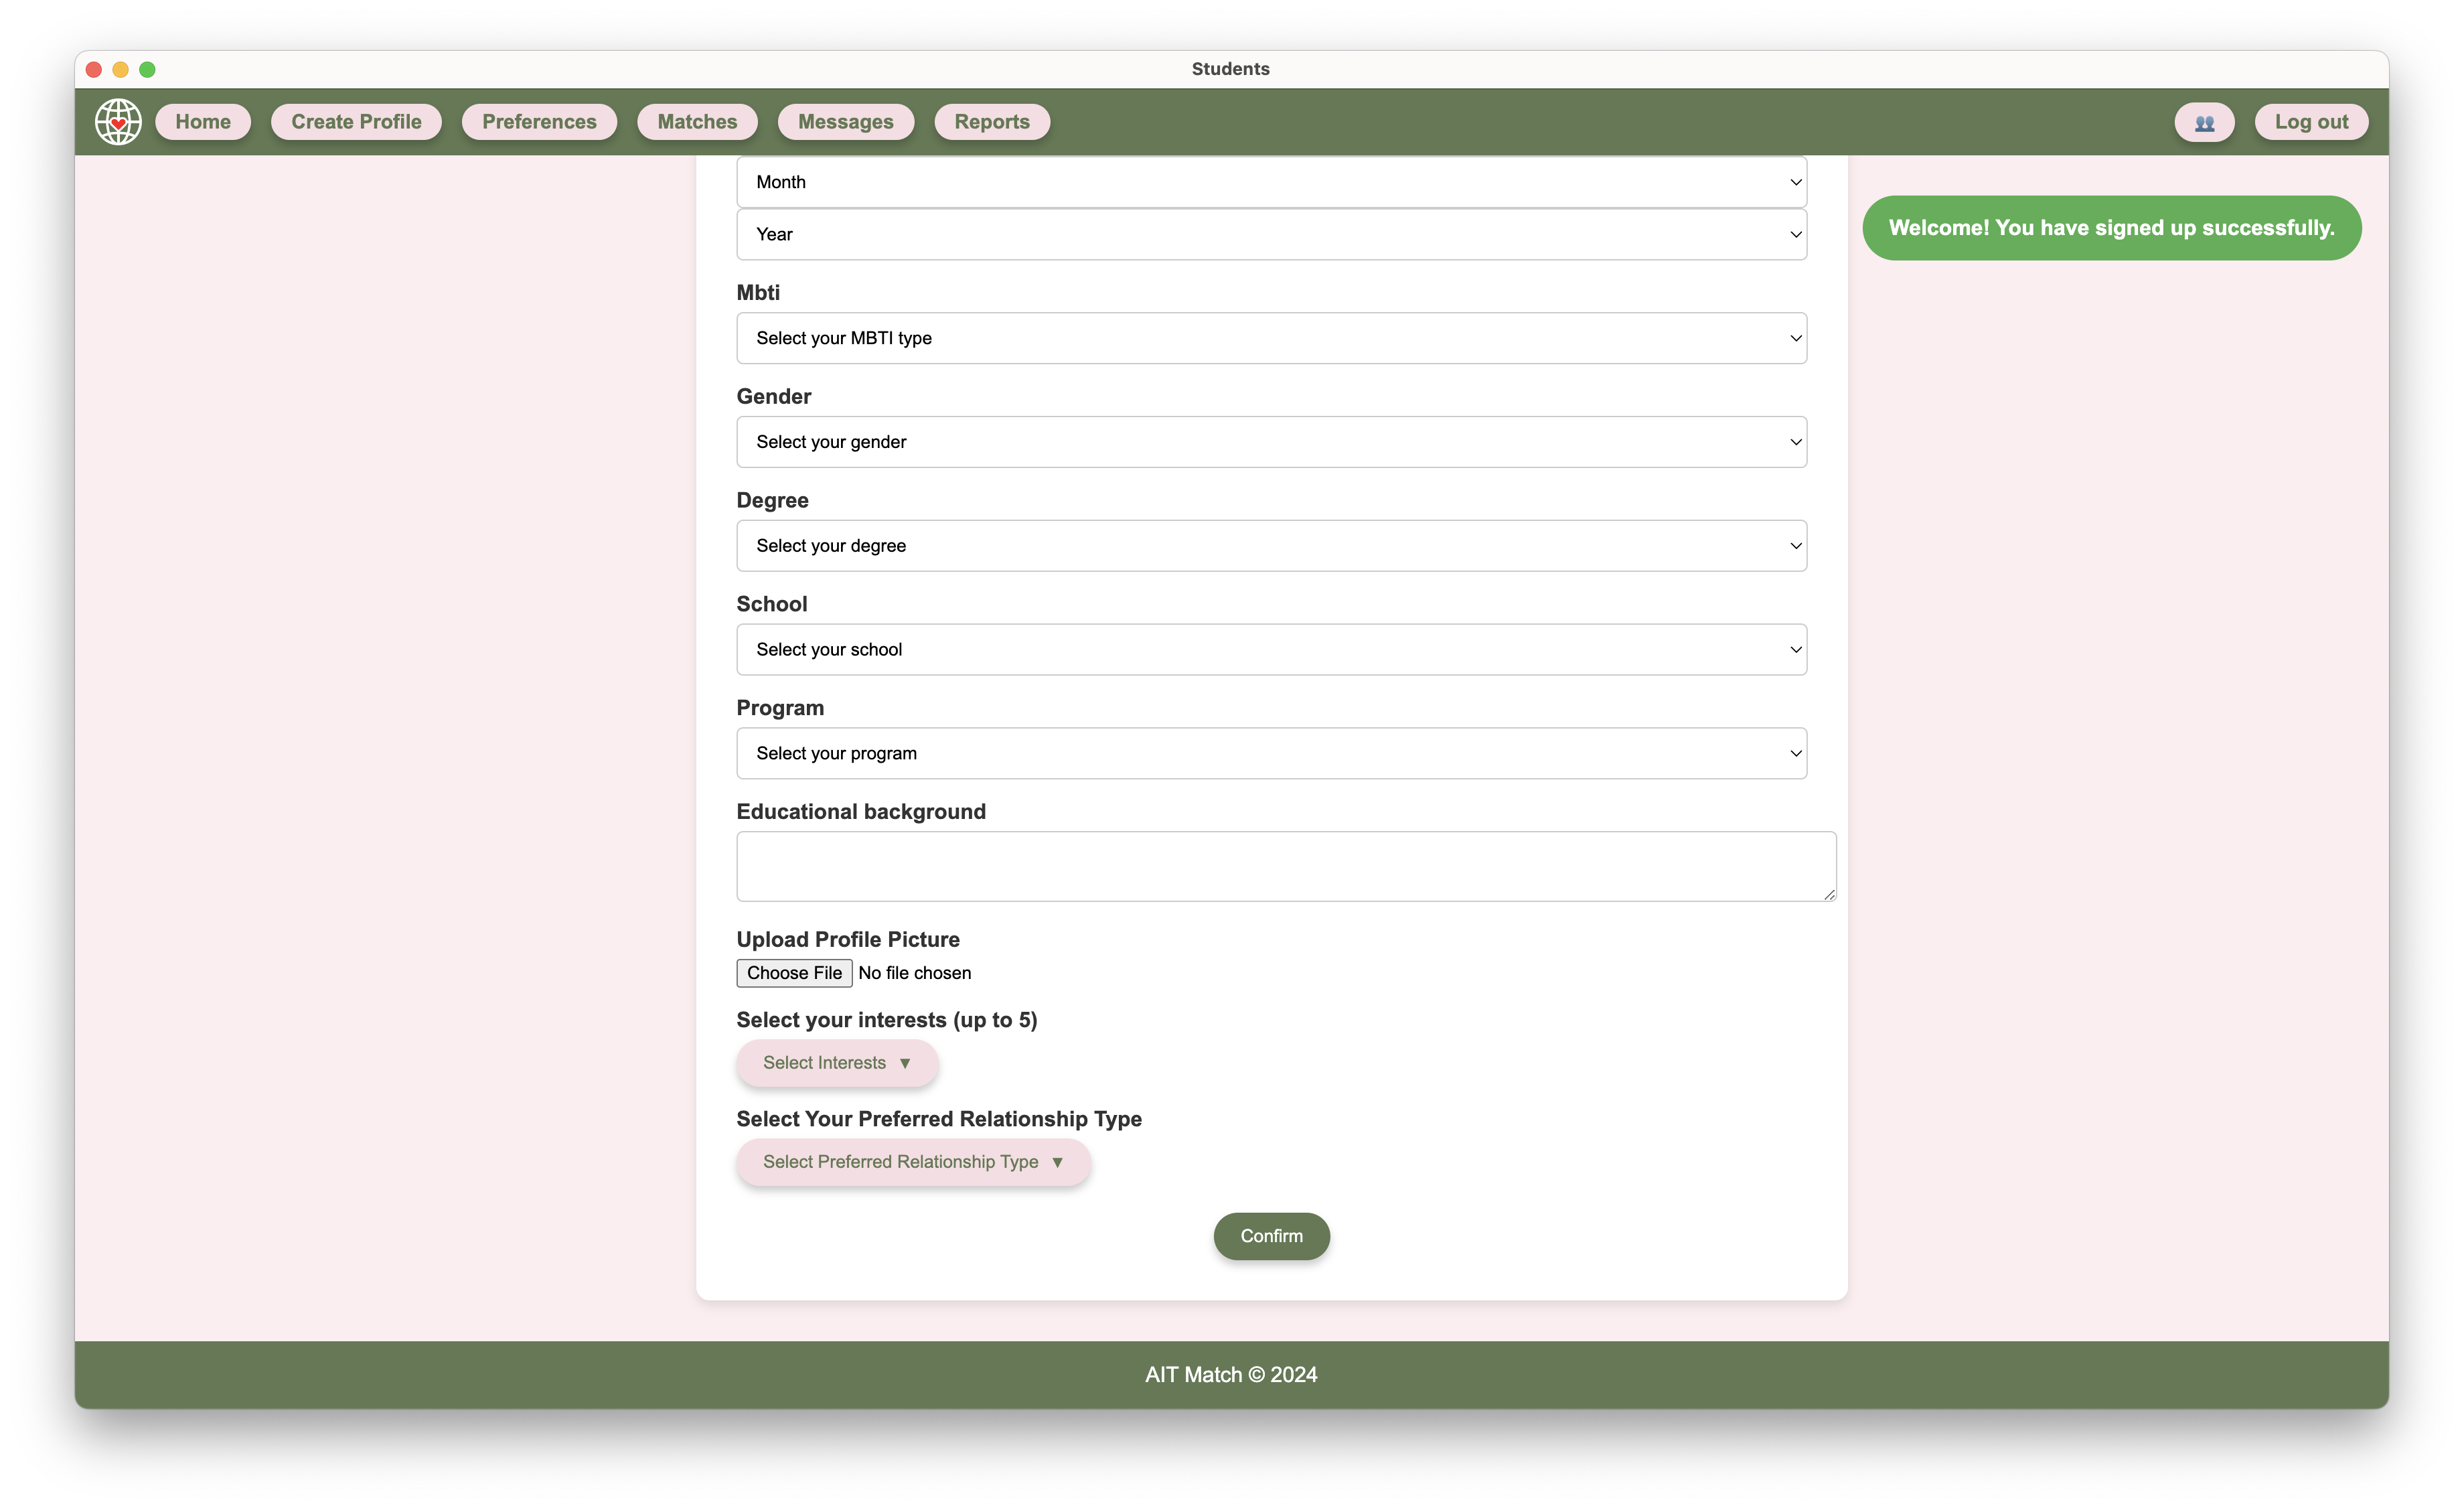
\includegraphics[width=5in]{figures/results/profiles/create-profile-page2.png} 
                \caption{Profile Creation Page (Continued).}
                \label{fig:create-profile-page2}
            \end{figure}

        \newpage
        \subsection{Profile: Validation of the Profile Creation Page}
        \begin{figure}[h]
                \centering
                \captionsetup{justification=centering, singlelinecheck=false, labelsep=space}
                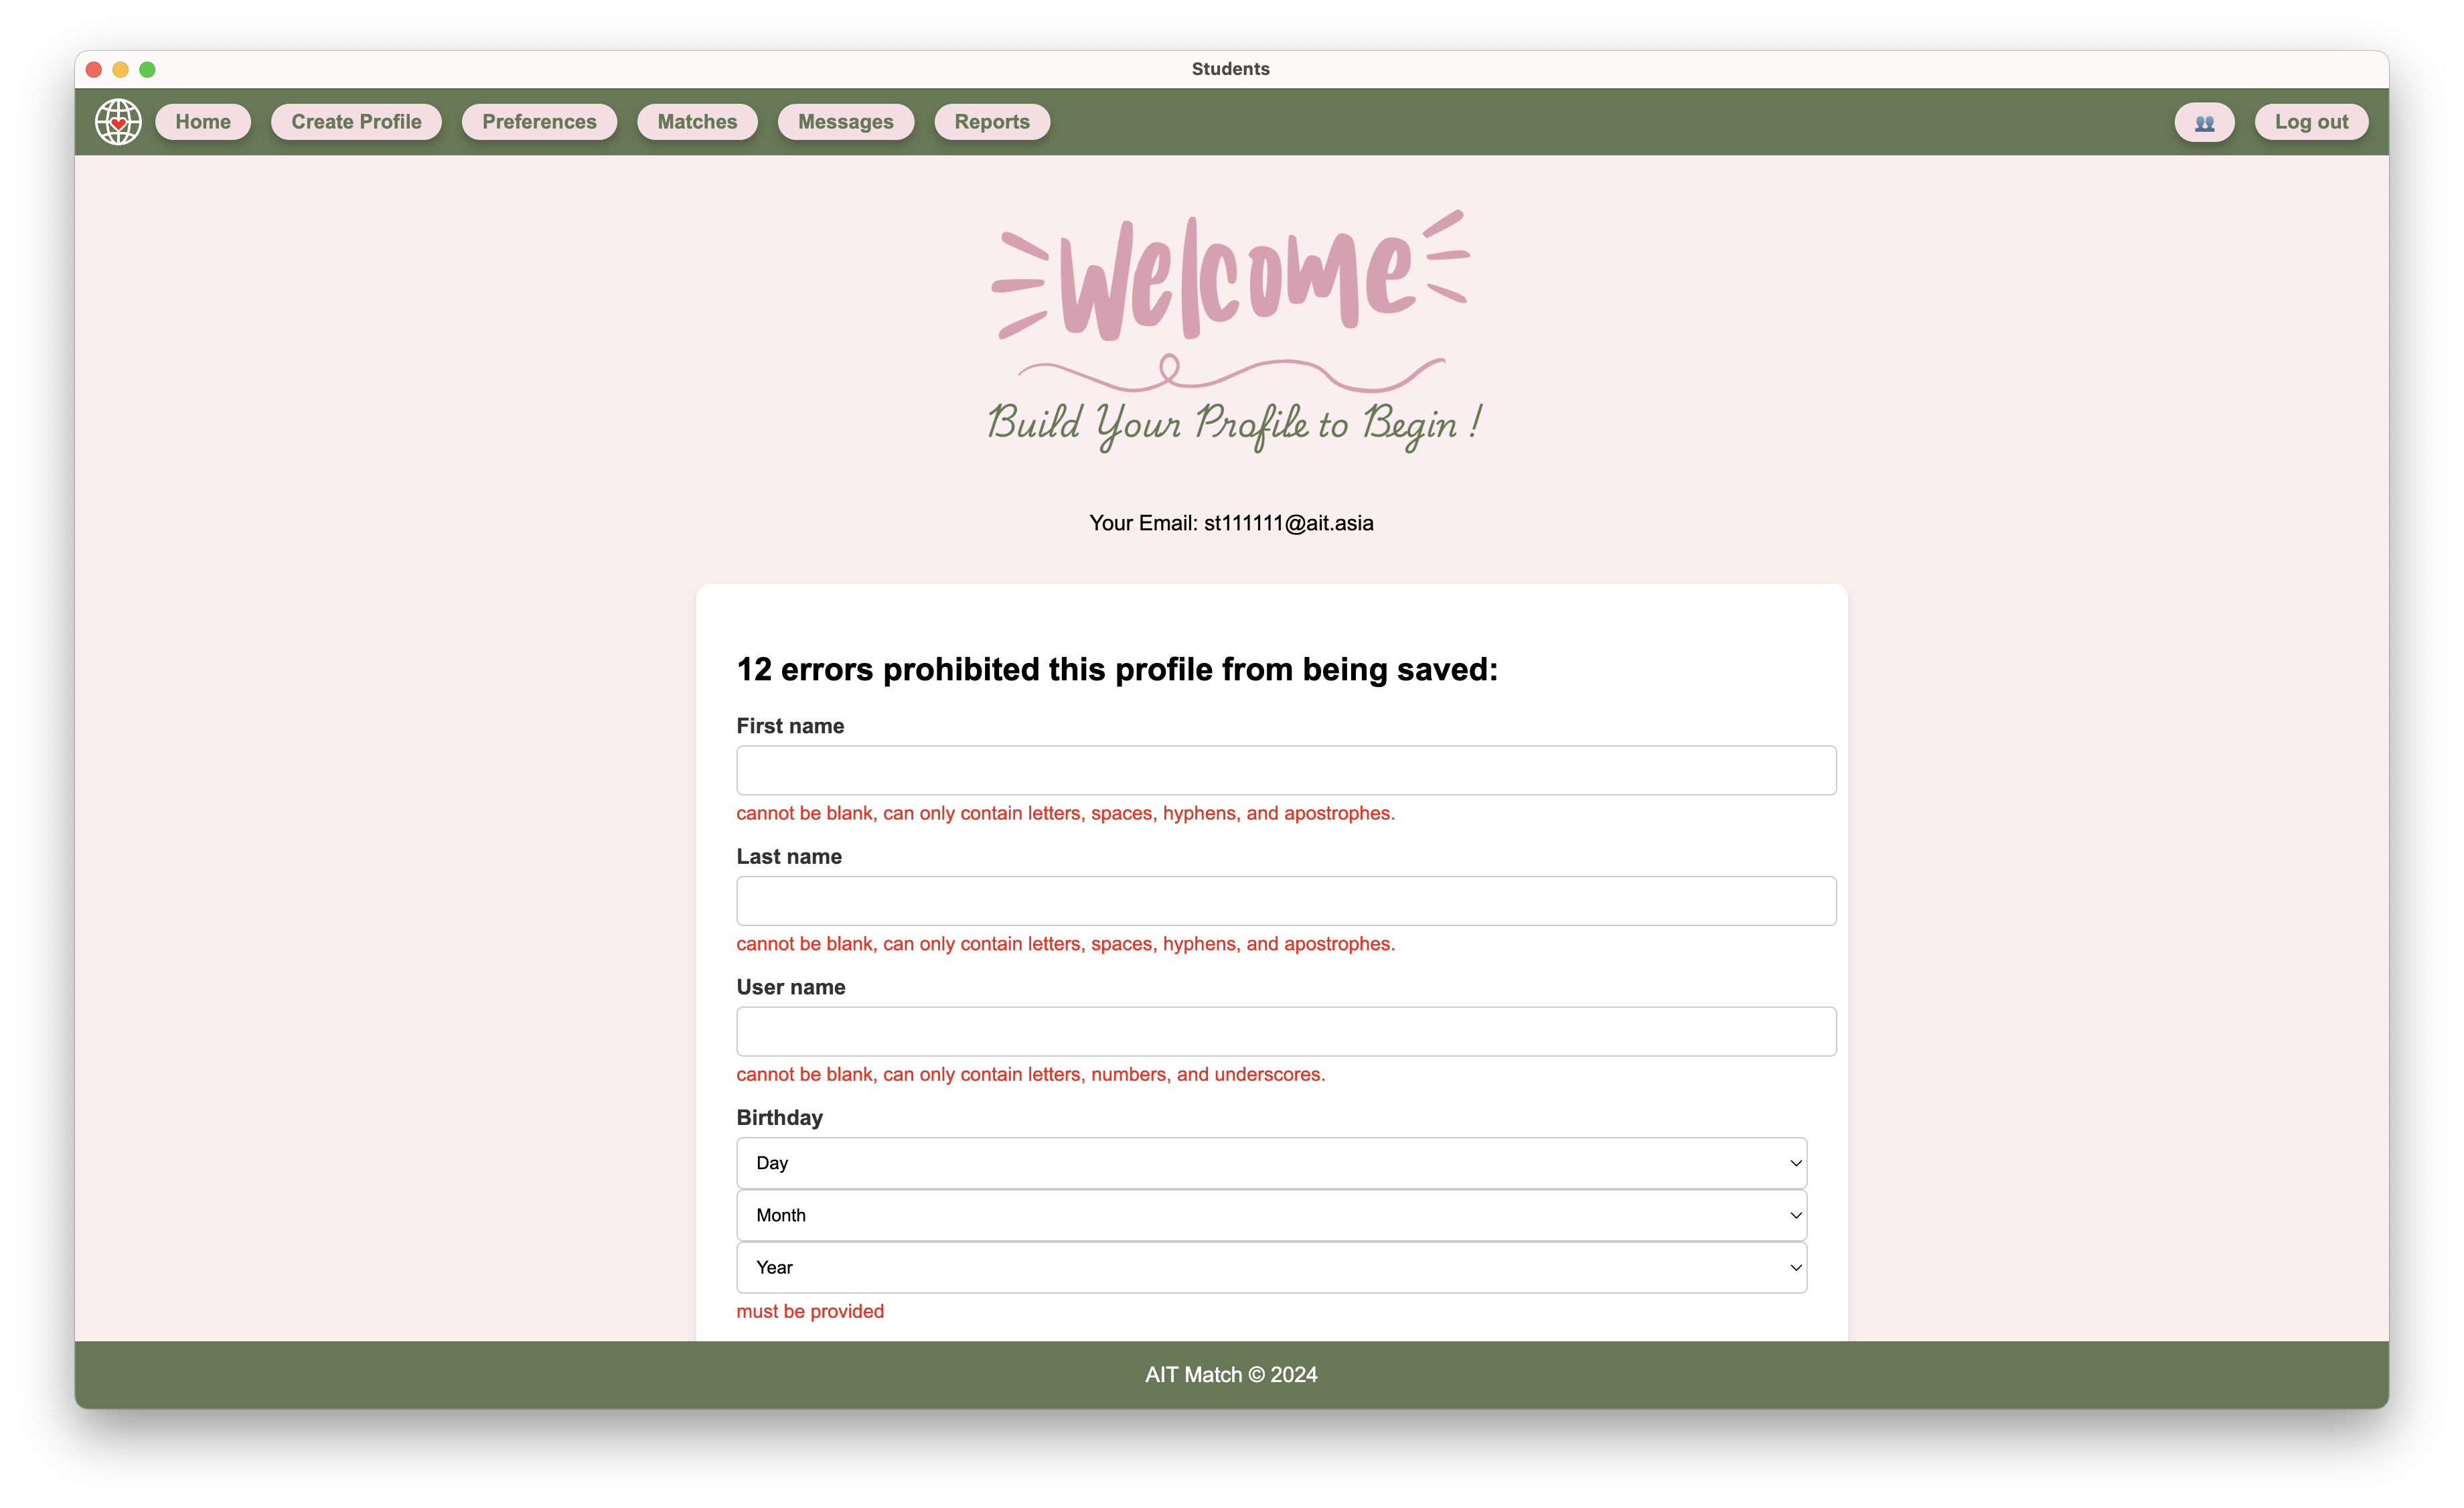
\includegraphics[width=5in]{figures/results/profiles/create-profile-error.png} 
                \caption{Validation of the Profile Creation Page.}
                \label{fig:create-profile-error}
            \end{figure}

        \subsection{Profile: Validation of the Profile Creation Page (Continued)}
        \begin{figure}[h]
                \centering
                \captionsetup{justification=centering, singlelinecheck=false, labelsep=space}
                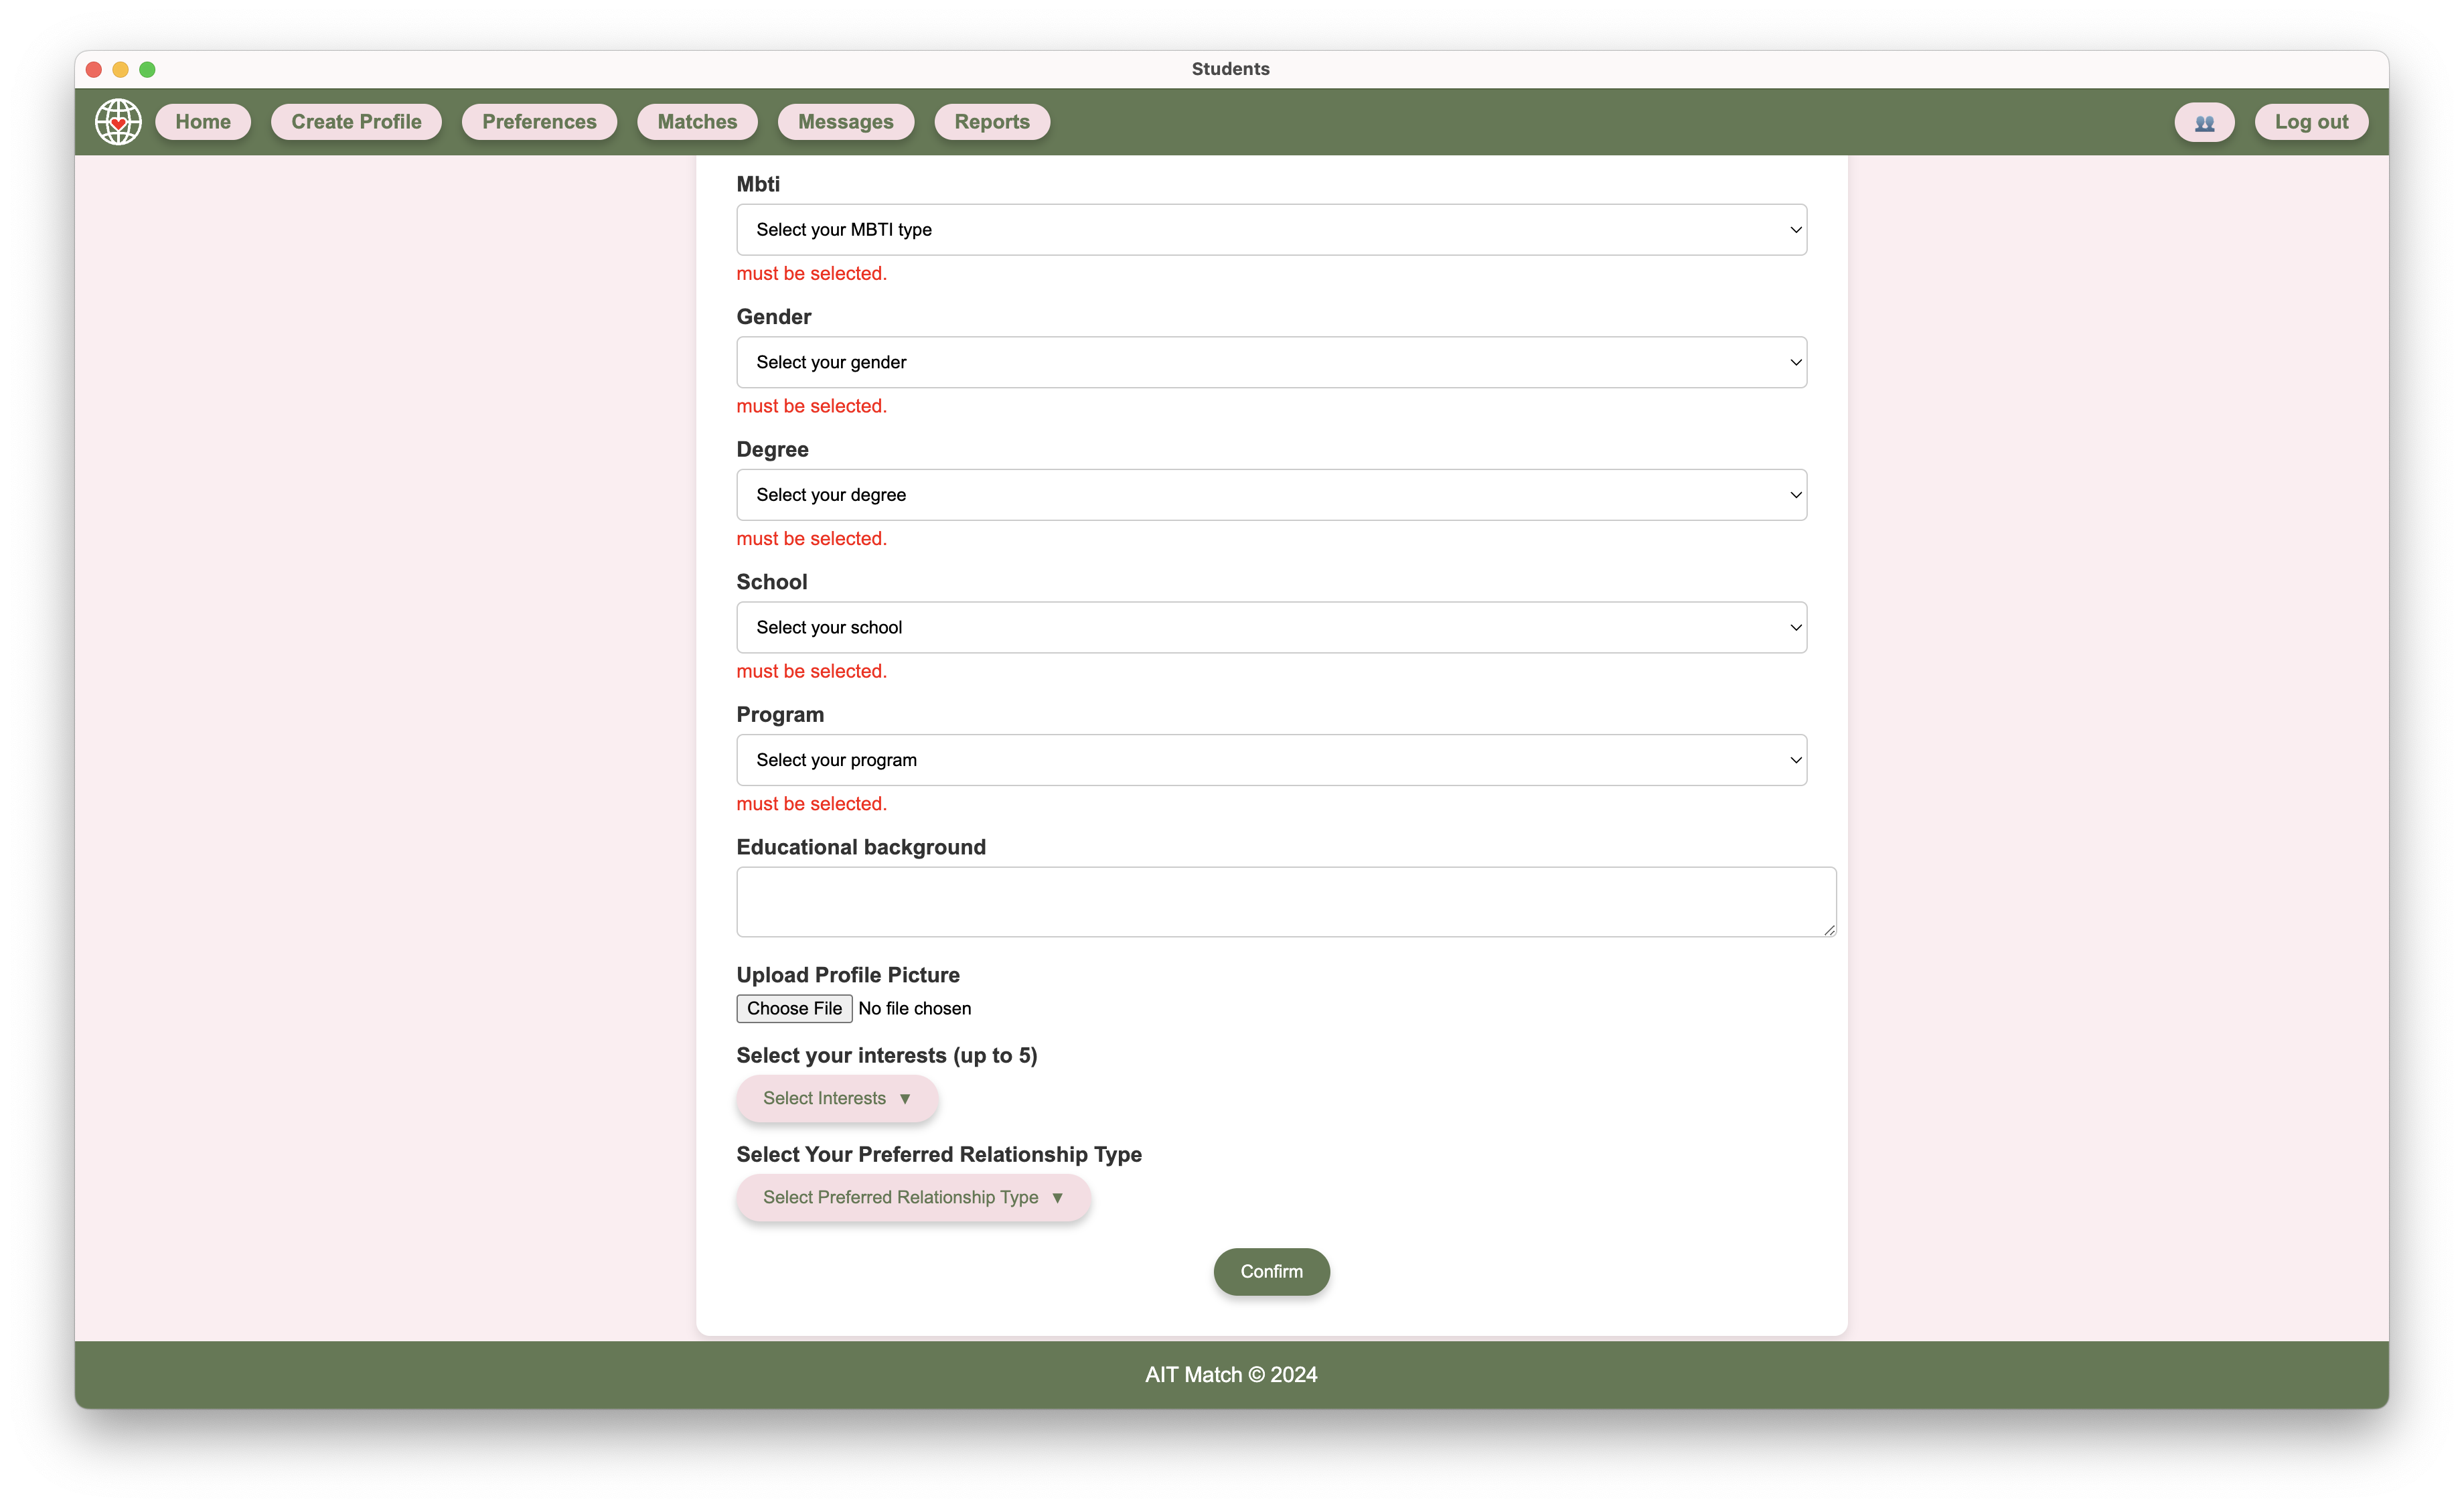
\includegraphics[width=5in]{figures/results/profiles/create-profile-error2.png} 
                \caption{Validation of the Profile Creation Page (Continued).}
                \label{fig:create-profile-error2}
            \end{figure}

        \newpage
        \subsection{Profile: Profile Edit Page}
        \begin{figure}[h]
                \centering
                \captionsetup{justification=centering, singlelinecheck=false, labelsep=space}
                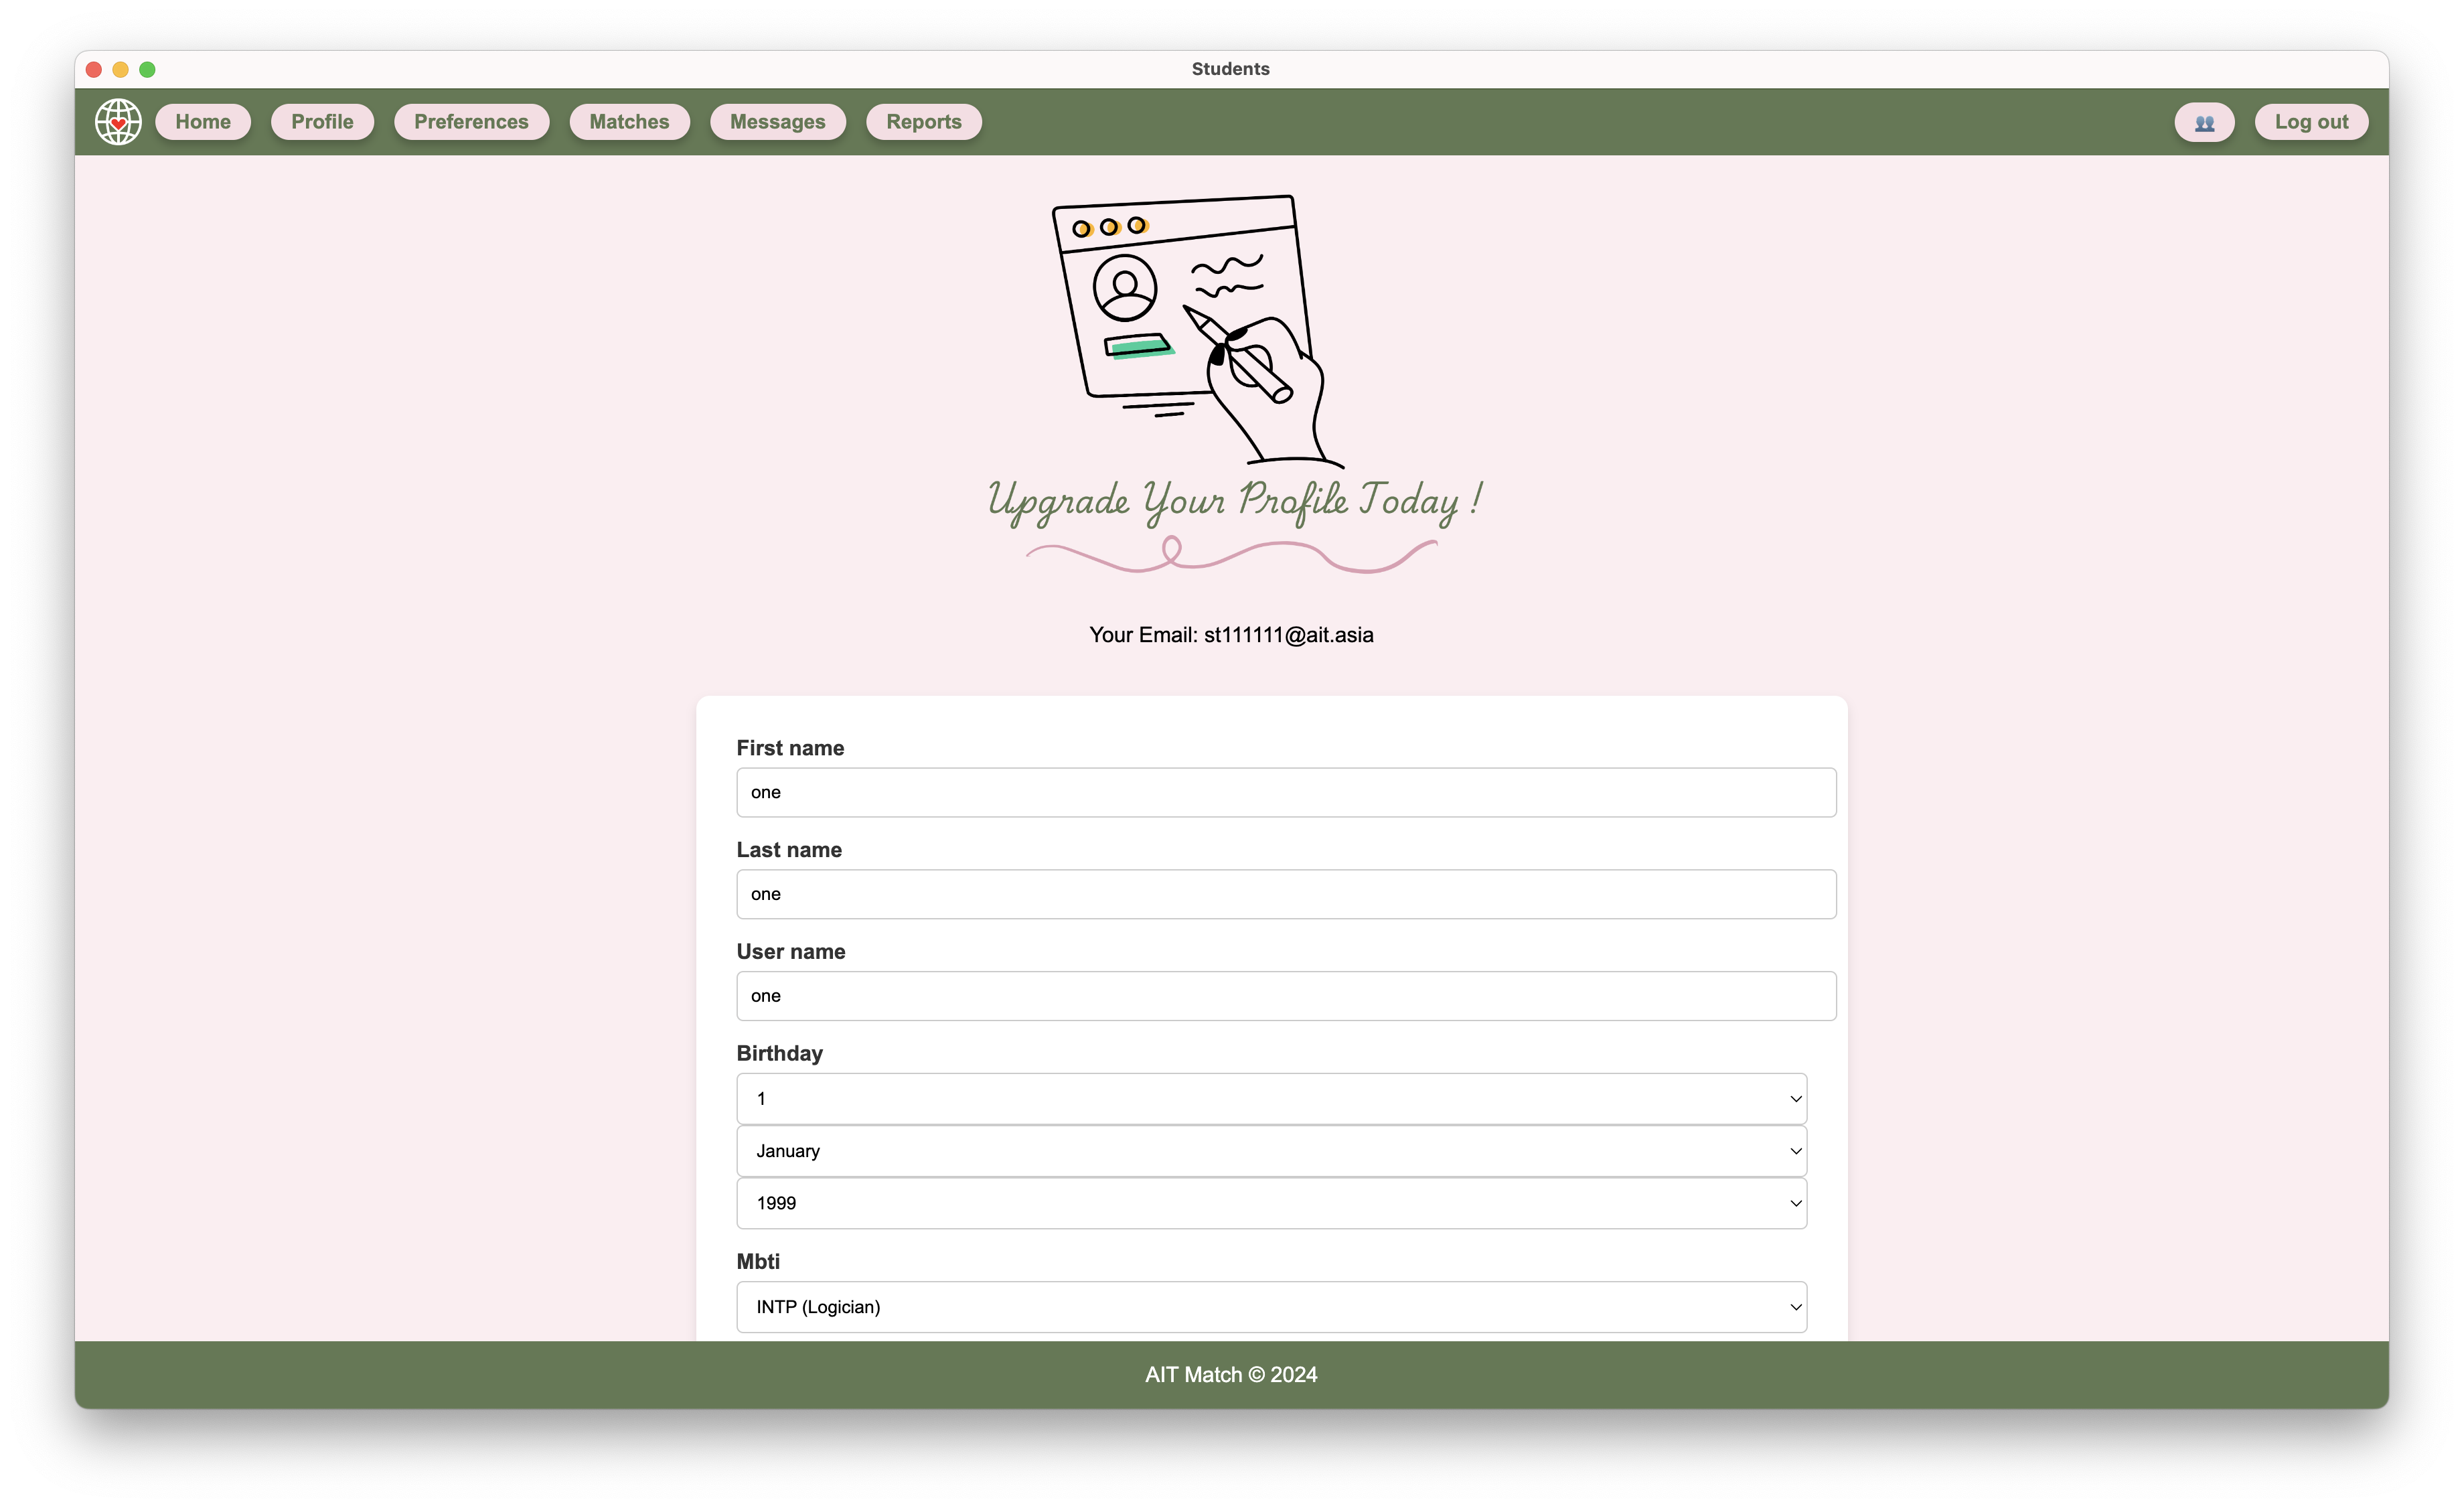
\includegraphics[width=5in]{figures/results/profiles/edit-profile-page.png} 
                \caption{Profile Edit Page.}
                \label{fig:edit-profile-page}
            \end{figure}

        \subsection{Profile: Profile Edit Page (Continued)}
        \begin{figure}[h]
                \centering
                \captionsetup{justification=centering, singlelinecheck=false, labelsep=space}
                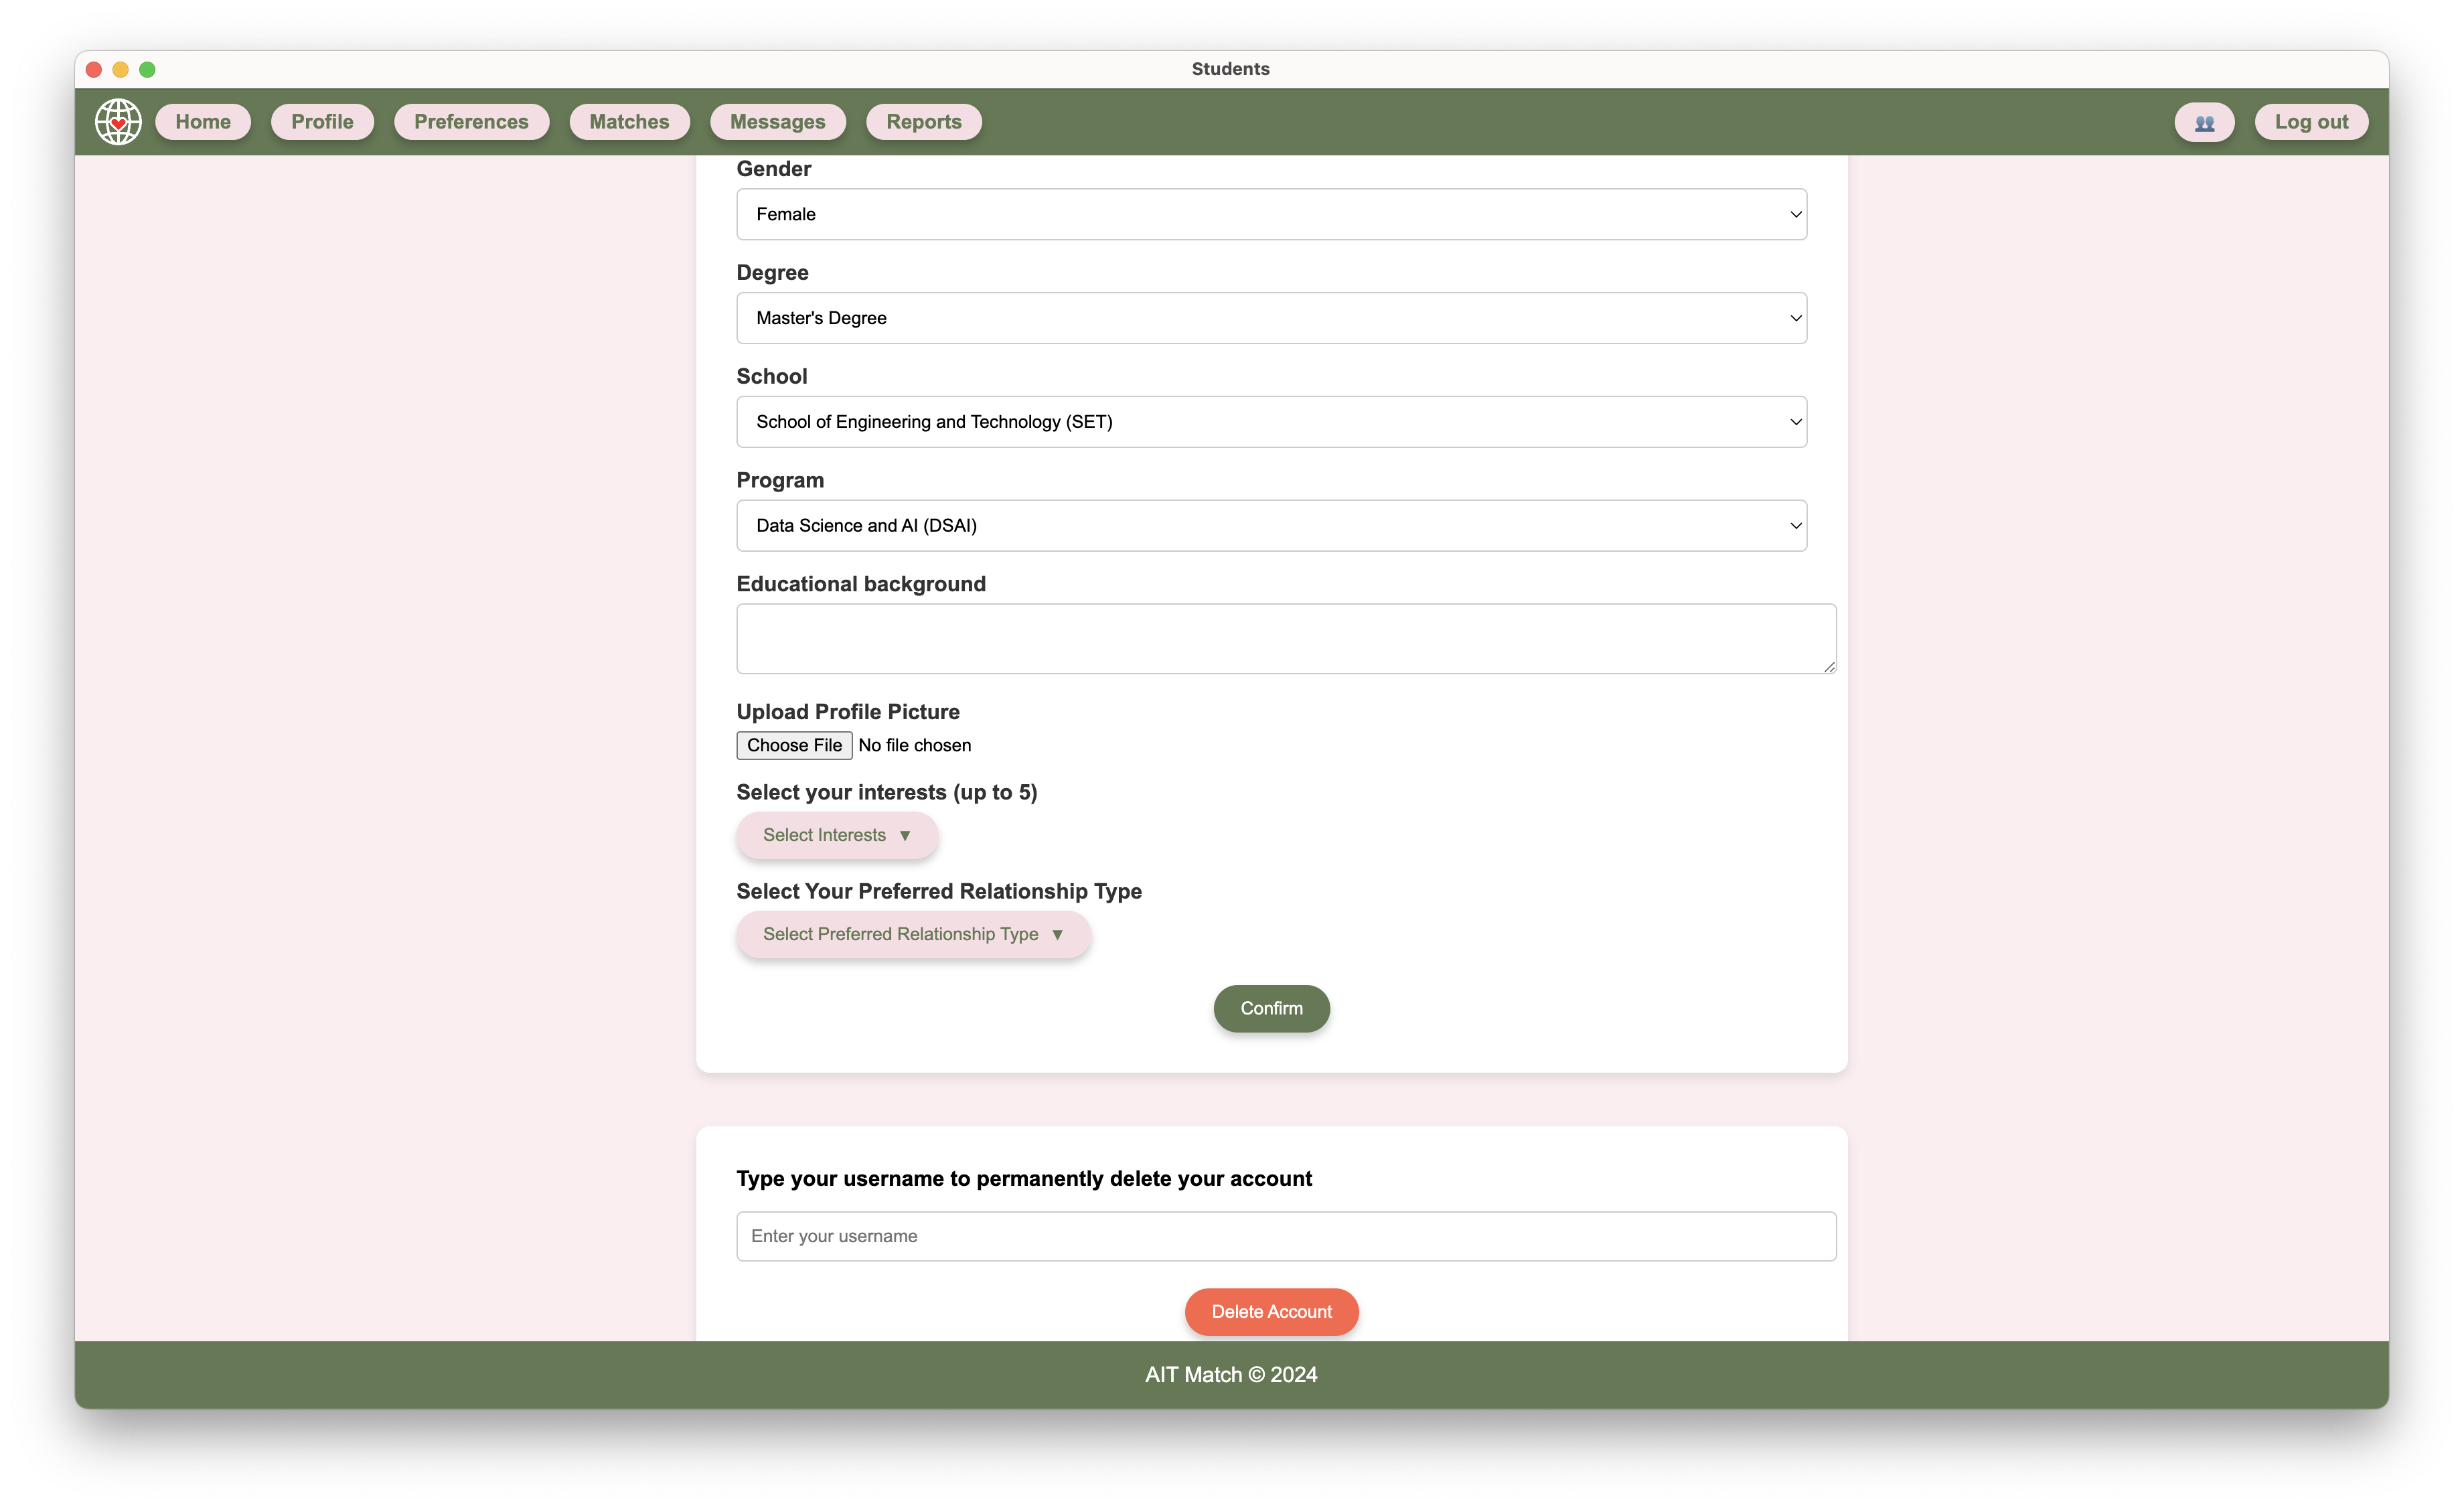
\includegraphics[width=5in]{figures/results/profiles/edit-profile-page2.png} 
                \caption{Profile Edit Page (Continued).}
                \label{fig:edit-profile-page2}
            \end{figure}

        \newpage
        \subsection{Profile: Profile Show Page}
        \begin{figure}[h]
                \centering
                \captionsetup{justification=centering, singlelinecheck=false, labelsep=space}
                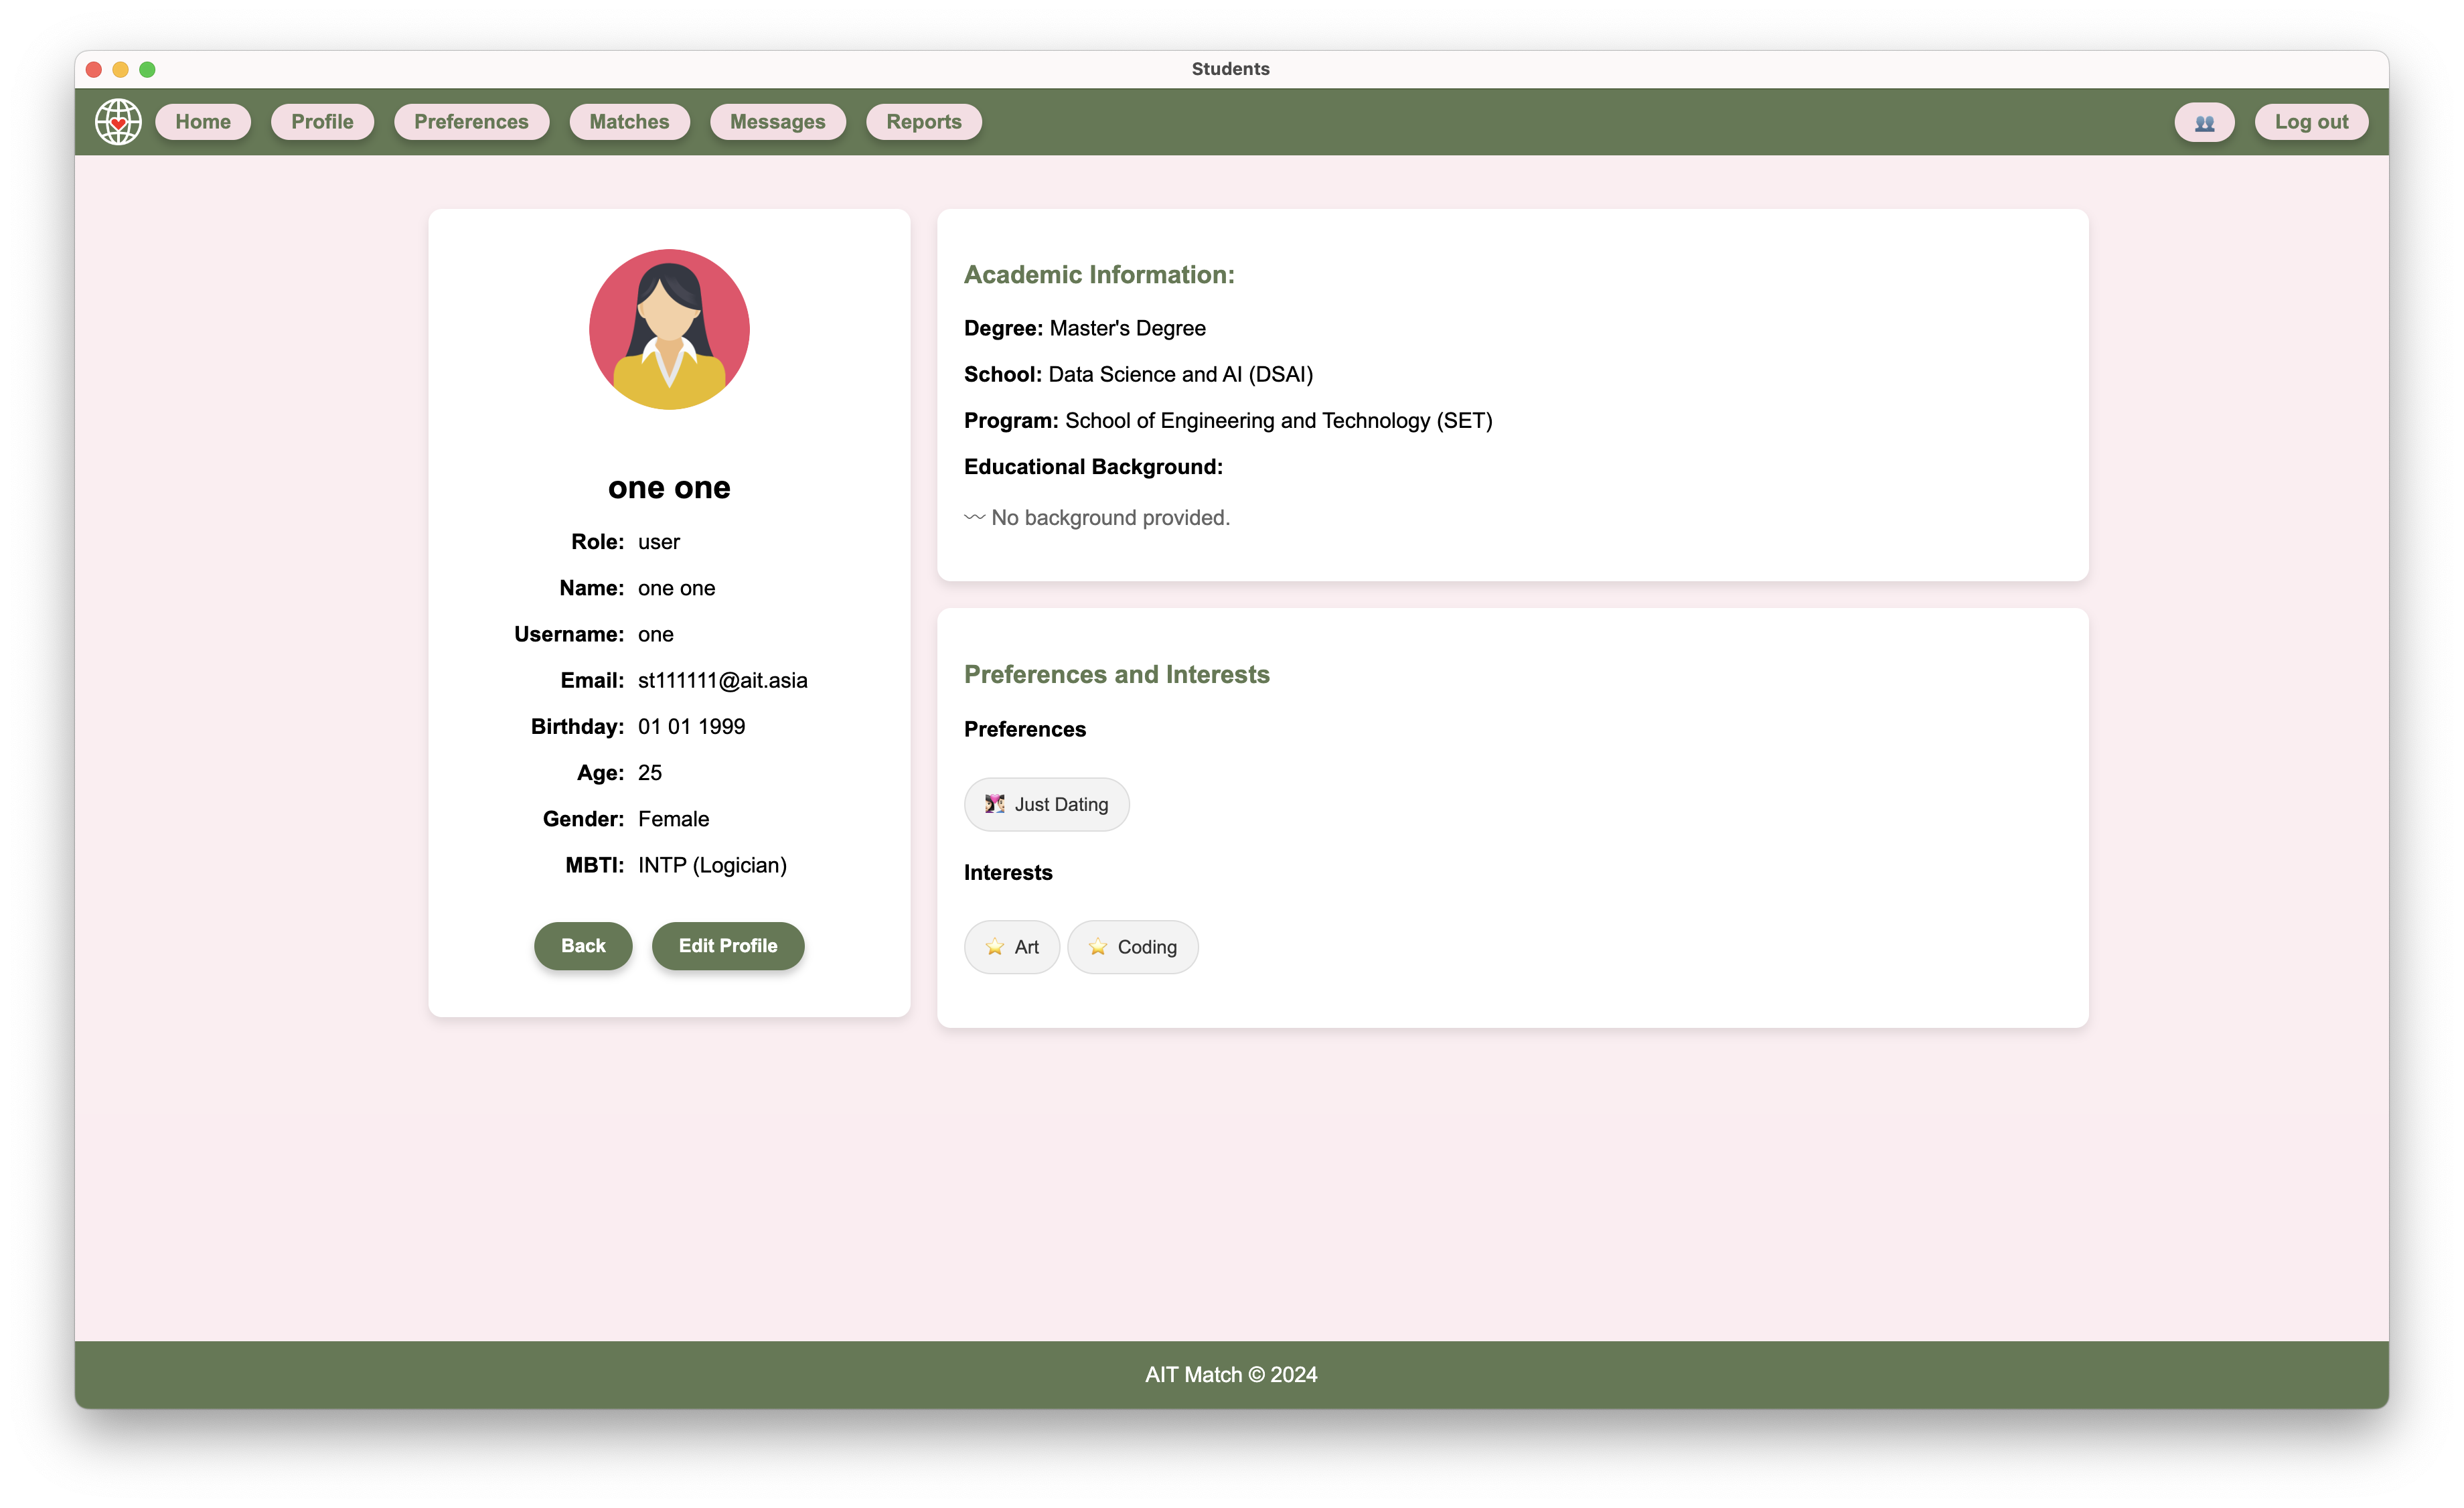
\includegraphics[width=5in]{figures/results/profiles/show-profile-page.png} 
                \caption{Profile Show Page.}
                \label{fig:show-profile-page}
            \end{figure}

        \subsection{Profile: Profile Index Page}
        \begin{figure}[h]
                \centering
                \captionsetup{justification=centering, singlelinecheck=false, labelsep=space}
                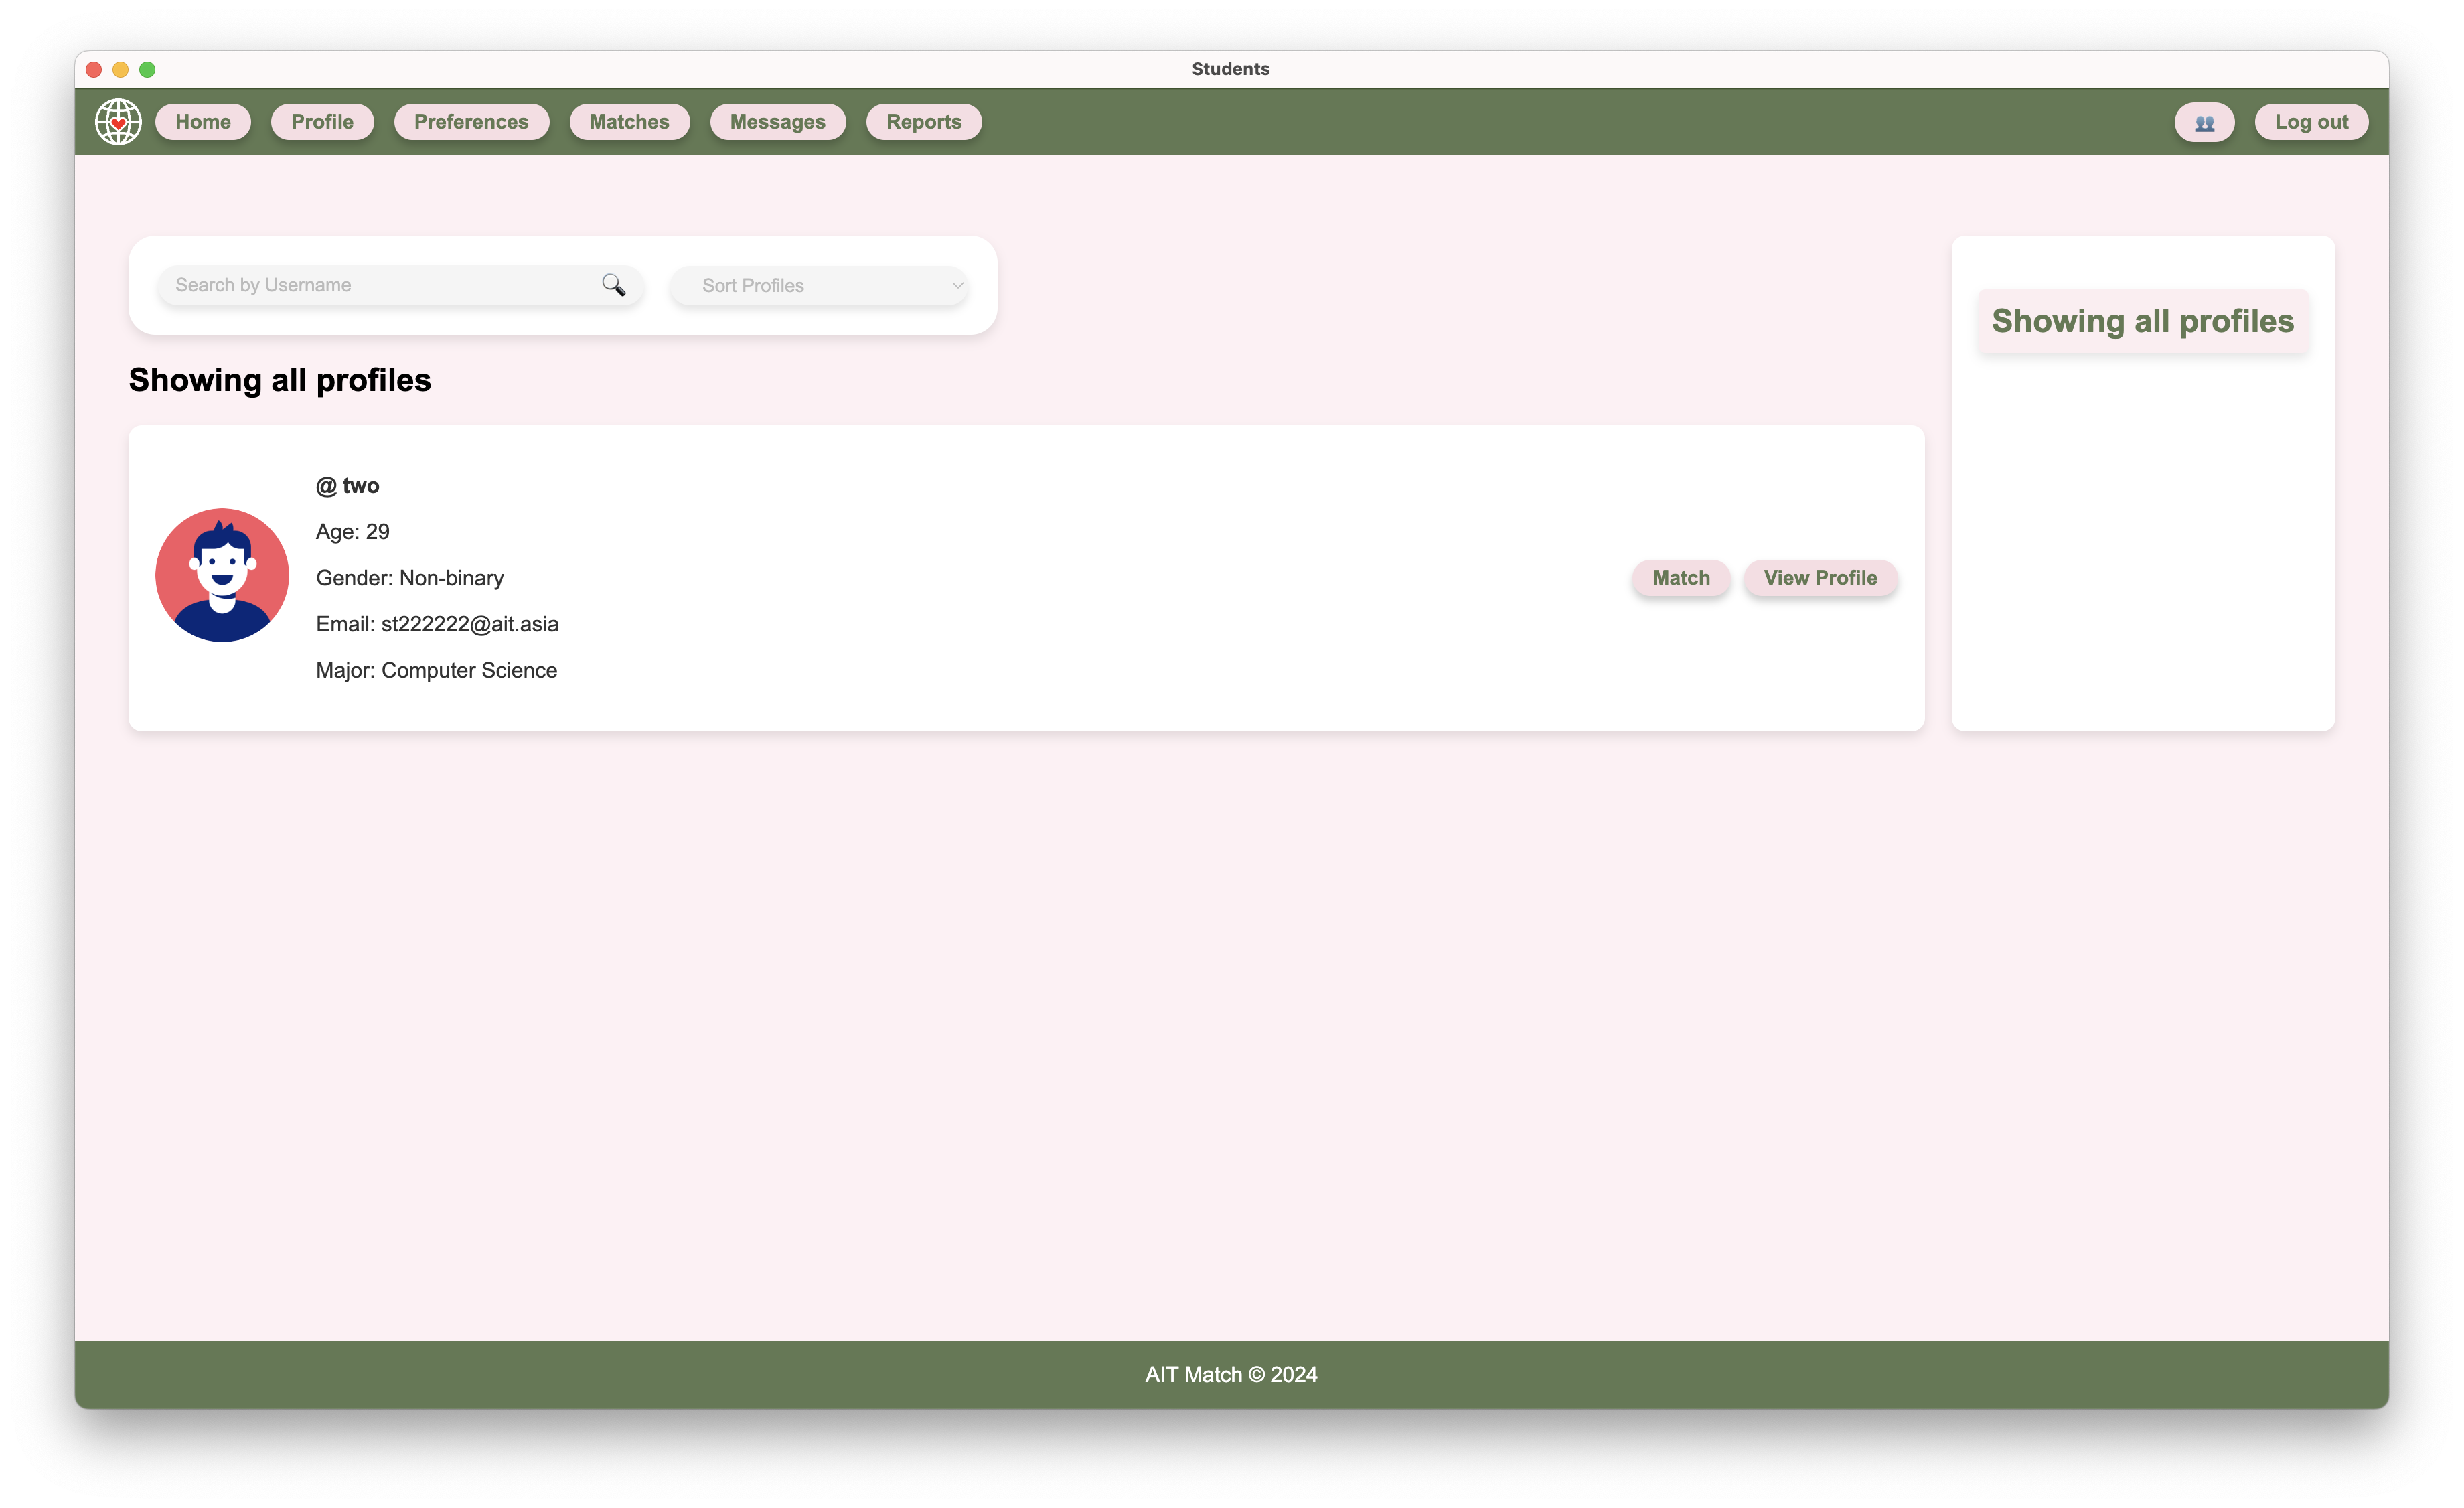
\includegraphics[width=5in]{figures/results/profiles/profile-index-page.png} 
                \caption{Profile Index Page.}
                \label{fig:profile-index-page}
            \end{figure}
% ------------------------------------------------- %
        \newpage
        \subsection{Preference: Preference Setup Page}
        \begin{figure}[h]
                \centering
                \captionsetup{justification=centering, singlelinecheck=false, labelsep=space}
                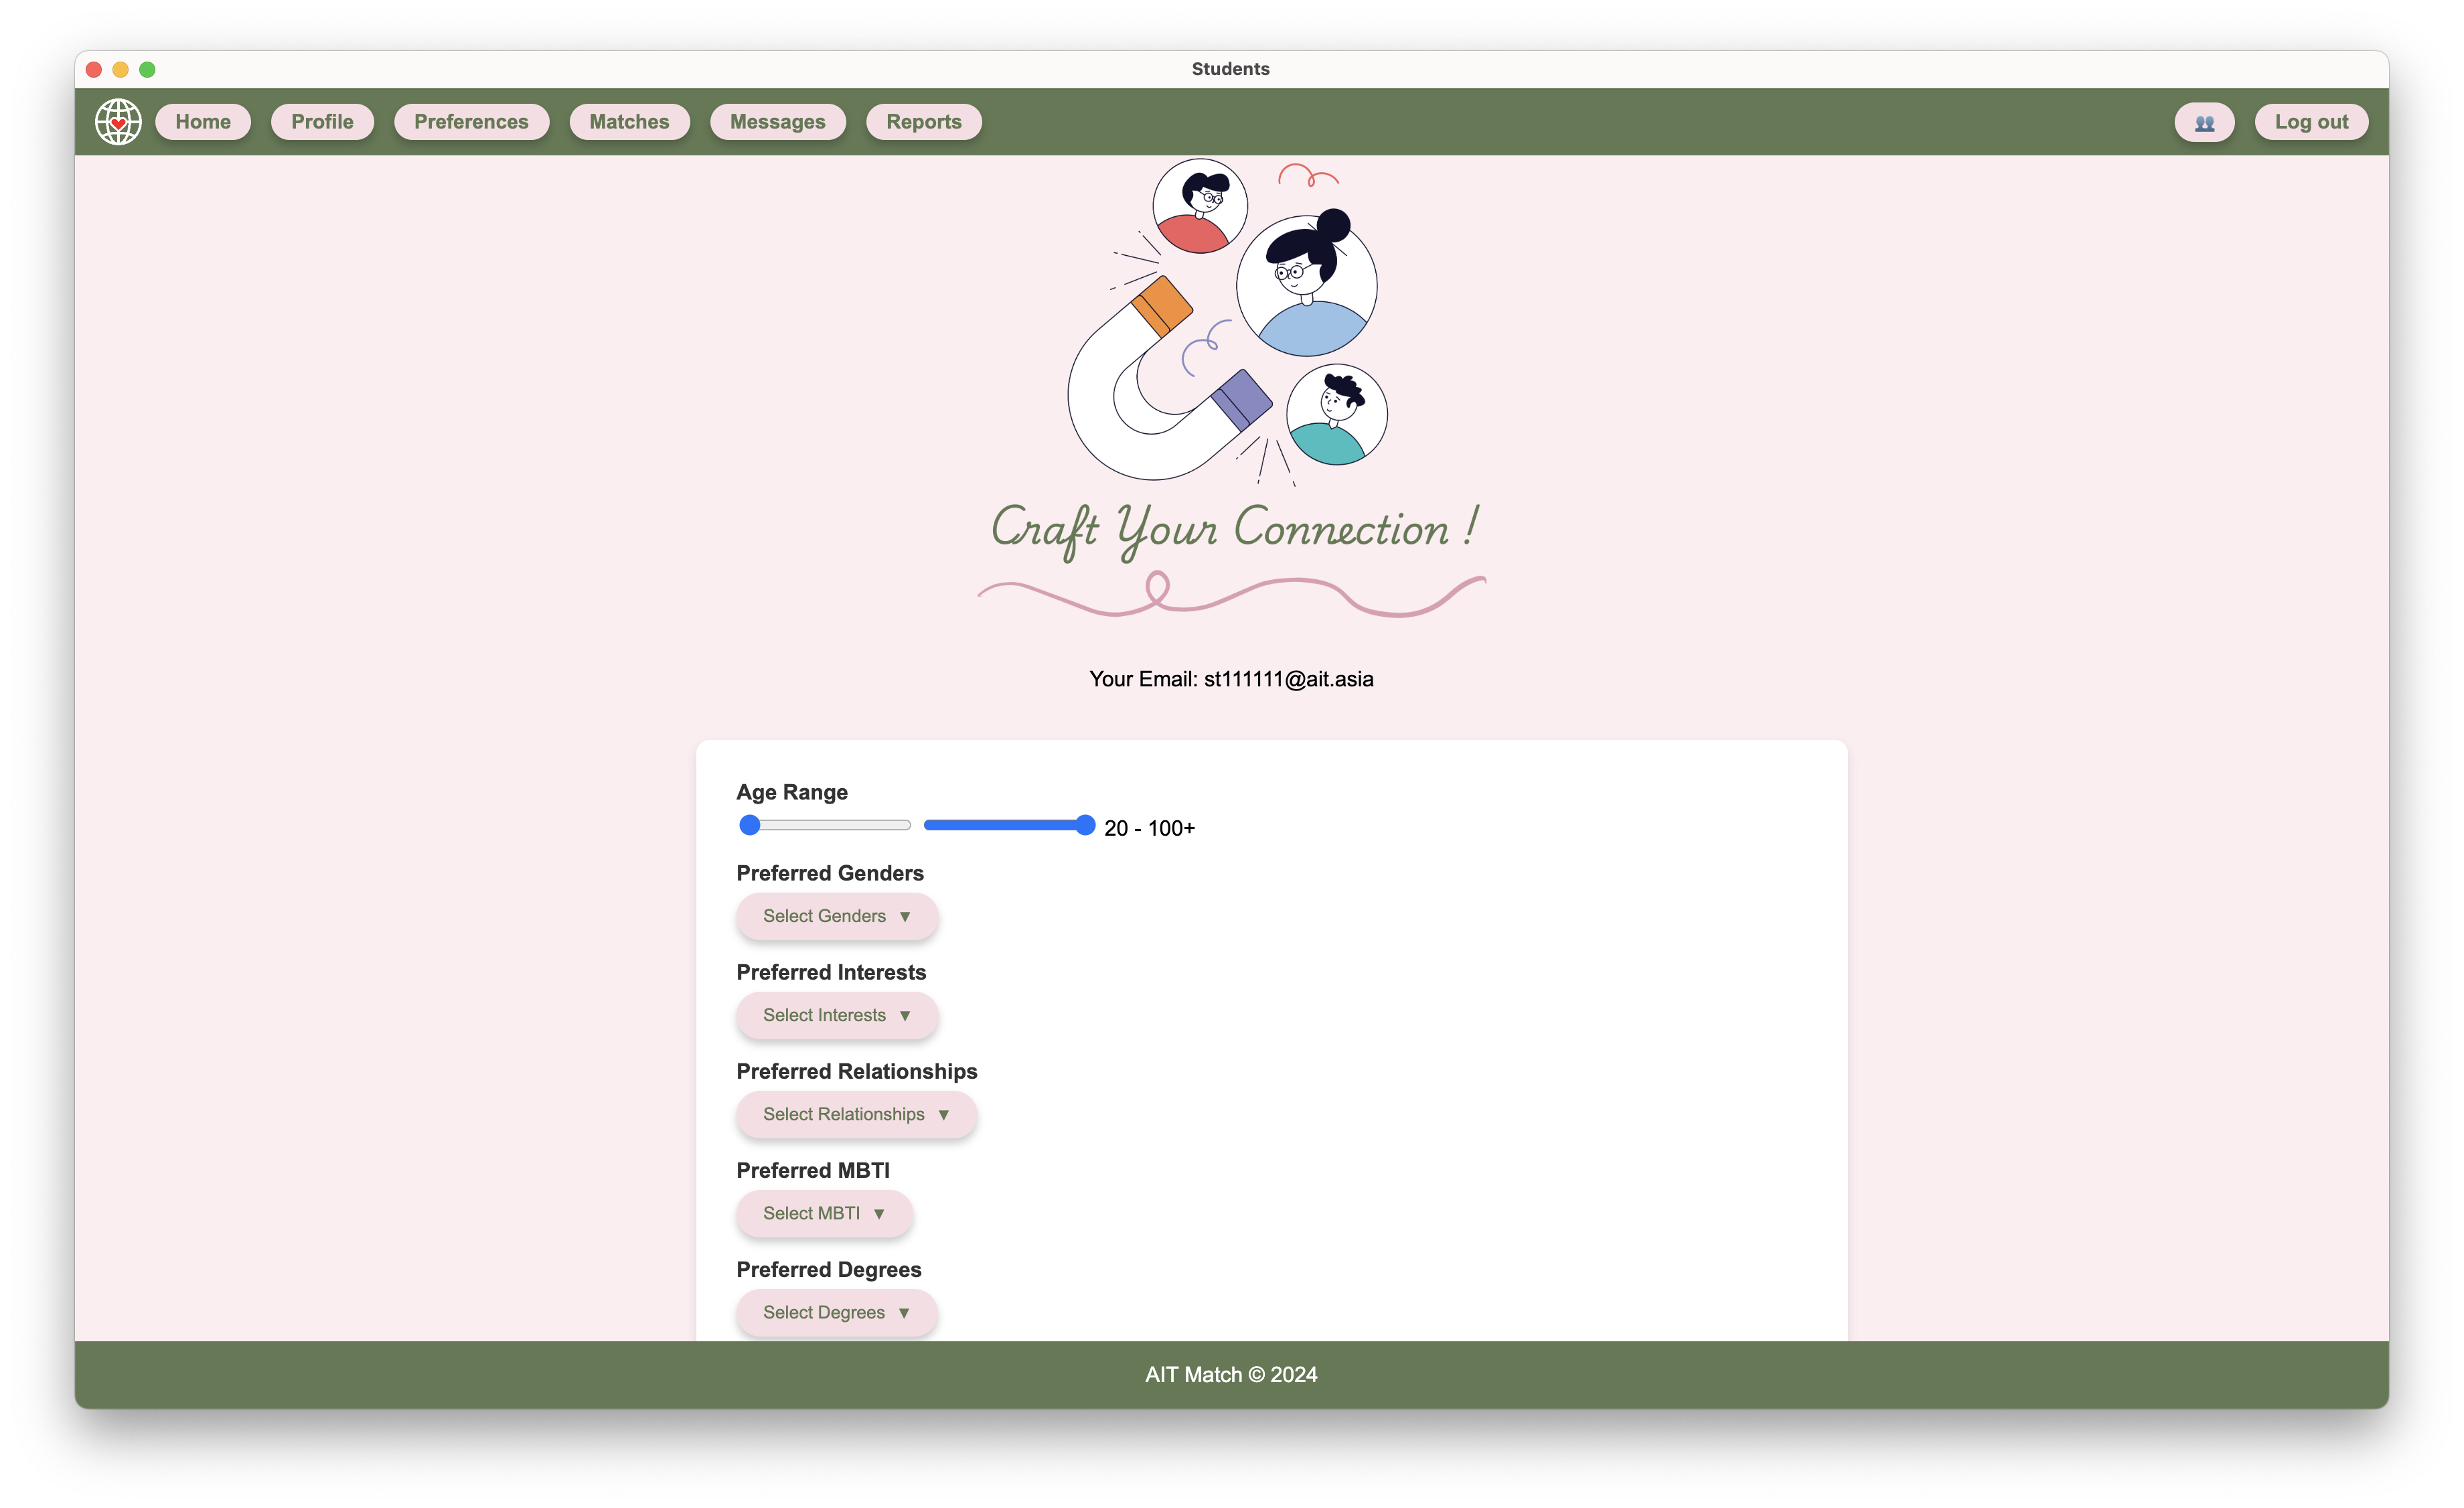
\includegraphics[width=5in]{figures/results/preferences/set-preference-page.png} 
                \caption{Preference Setup Page.}
                \label{fig:set-preference-page-2}
            \end{figure}

        \subsection{Preference: Preference Setup Page (Continued)}
        \begin{figure}[h]
                \centering
                \captionsetup{justification=centering, singlelinecheck=false, labelsep=space}
                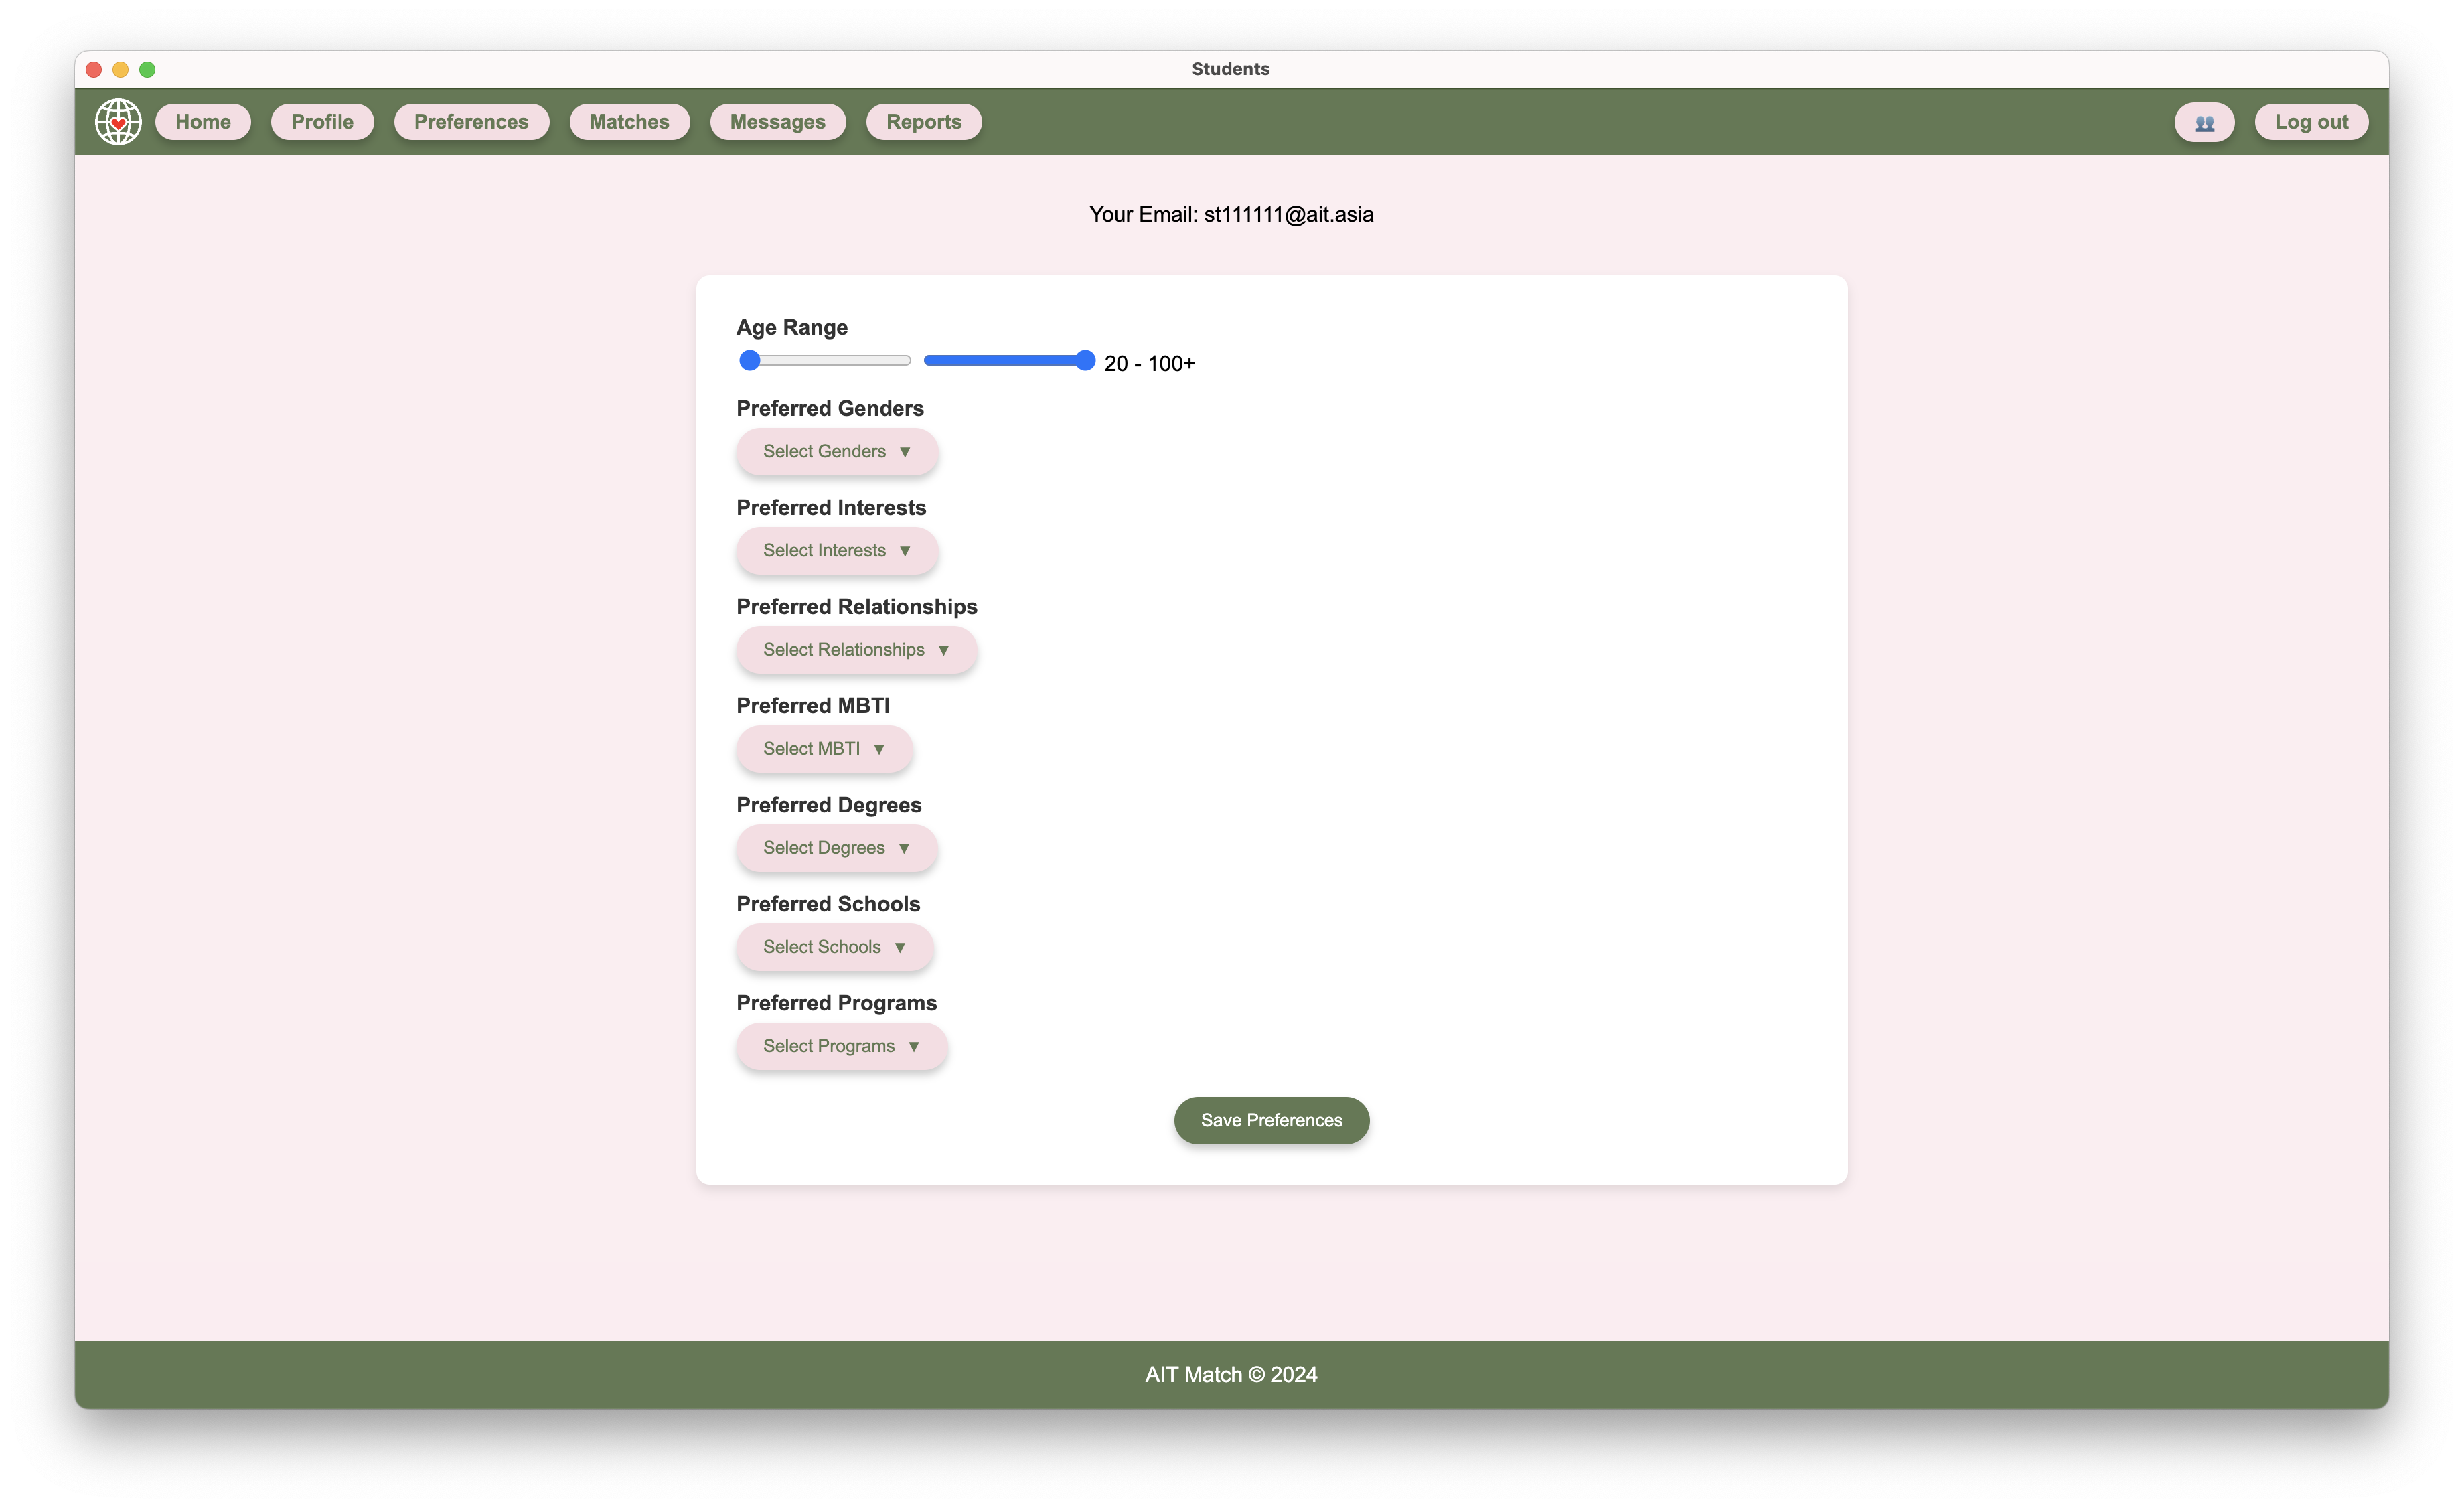
\includegraphics[width=5in]{figures/results/preferences/set-preference-page-2.png} 
                \caption{Preference Setup Page (Continued).}
                \label{fig:set-preference-page-2}
            \end{figure}
% ------------------------------------------------- %
        \newpage
        \subsection{Match: No Match Requests Page}
        \begin{figure}[h]
                \centering
                \captionsetup{justification=centering, singlelinecheck=false, labelsep=space}
                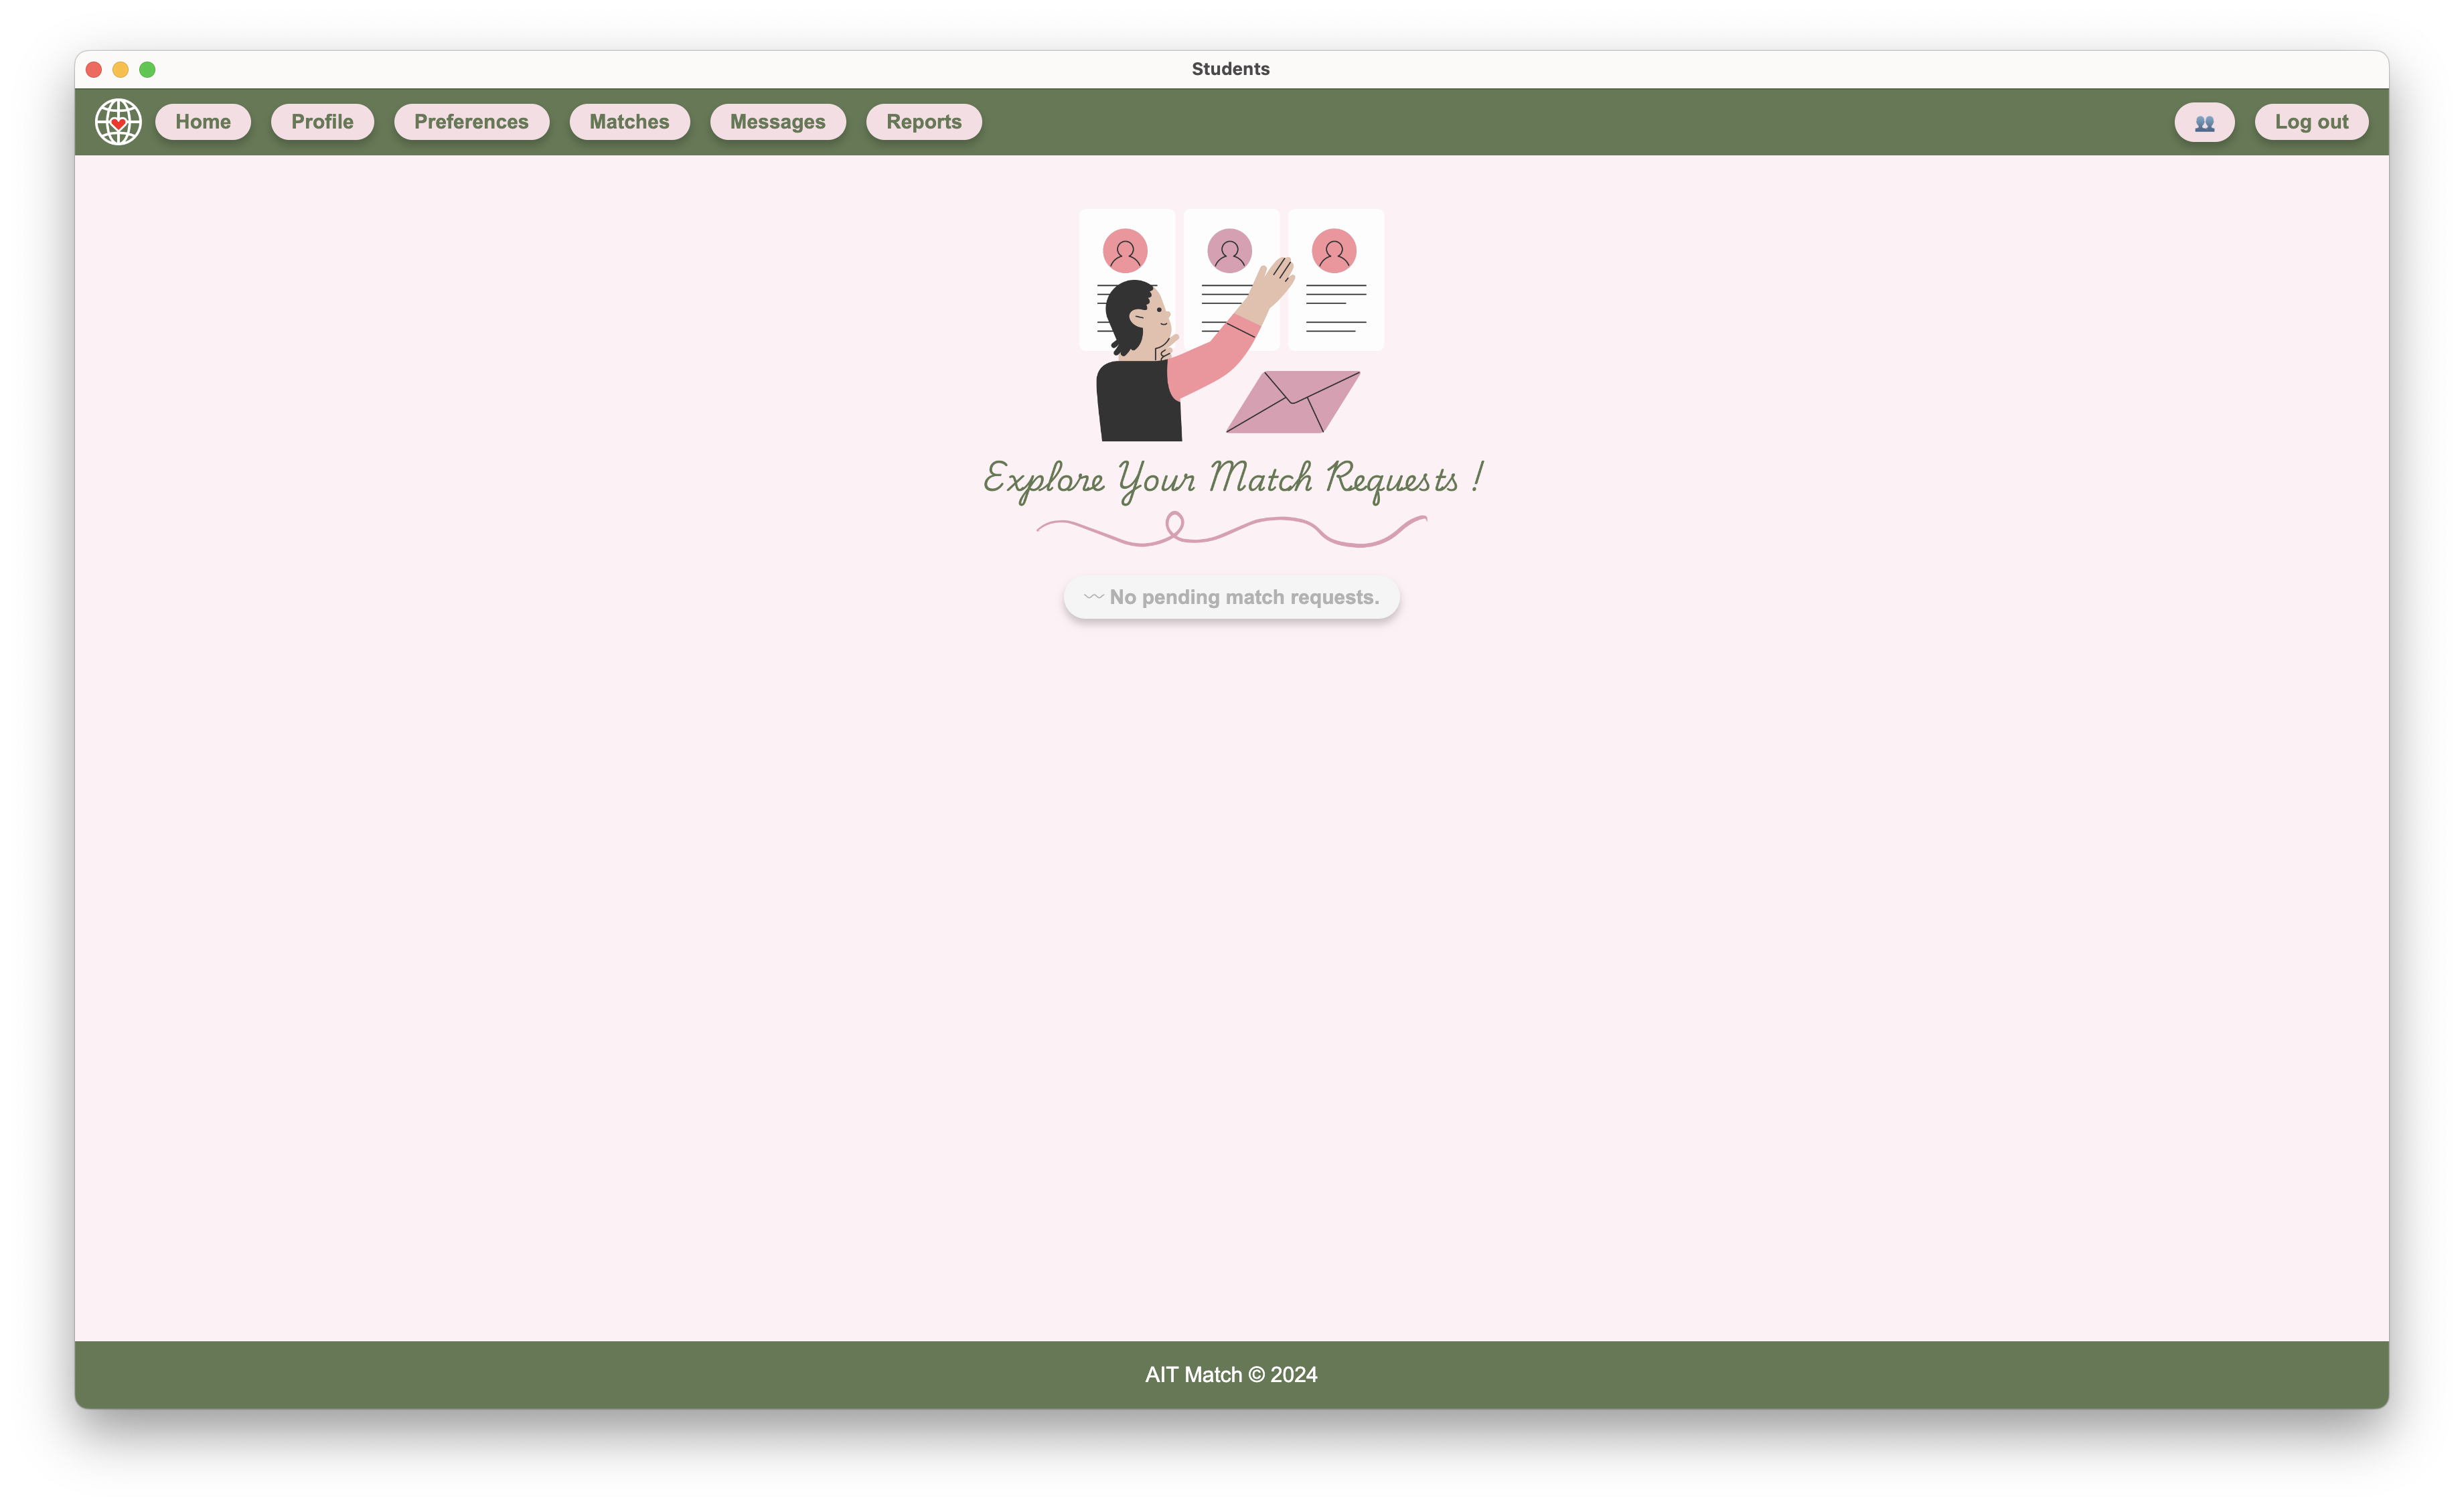
\includegraphics[width=5in]{figures/results/matches/no-match-request-page.png} 
                \caption{No Match Requests Page.}
                \label{fig:no-match-request-page}
            \end{figure}

        \subsection{Match: Match Requests Page}
        \begin{figure}[h]
                \centering
                \captionsetup{justification=centering, singlelinecheck=false, labelsep=space}
                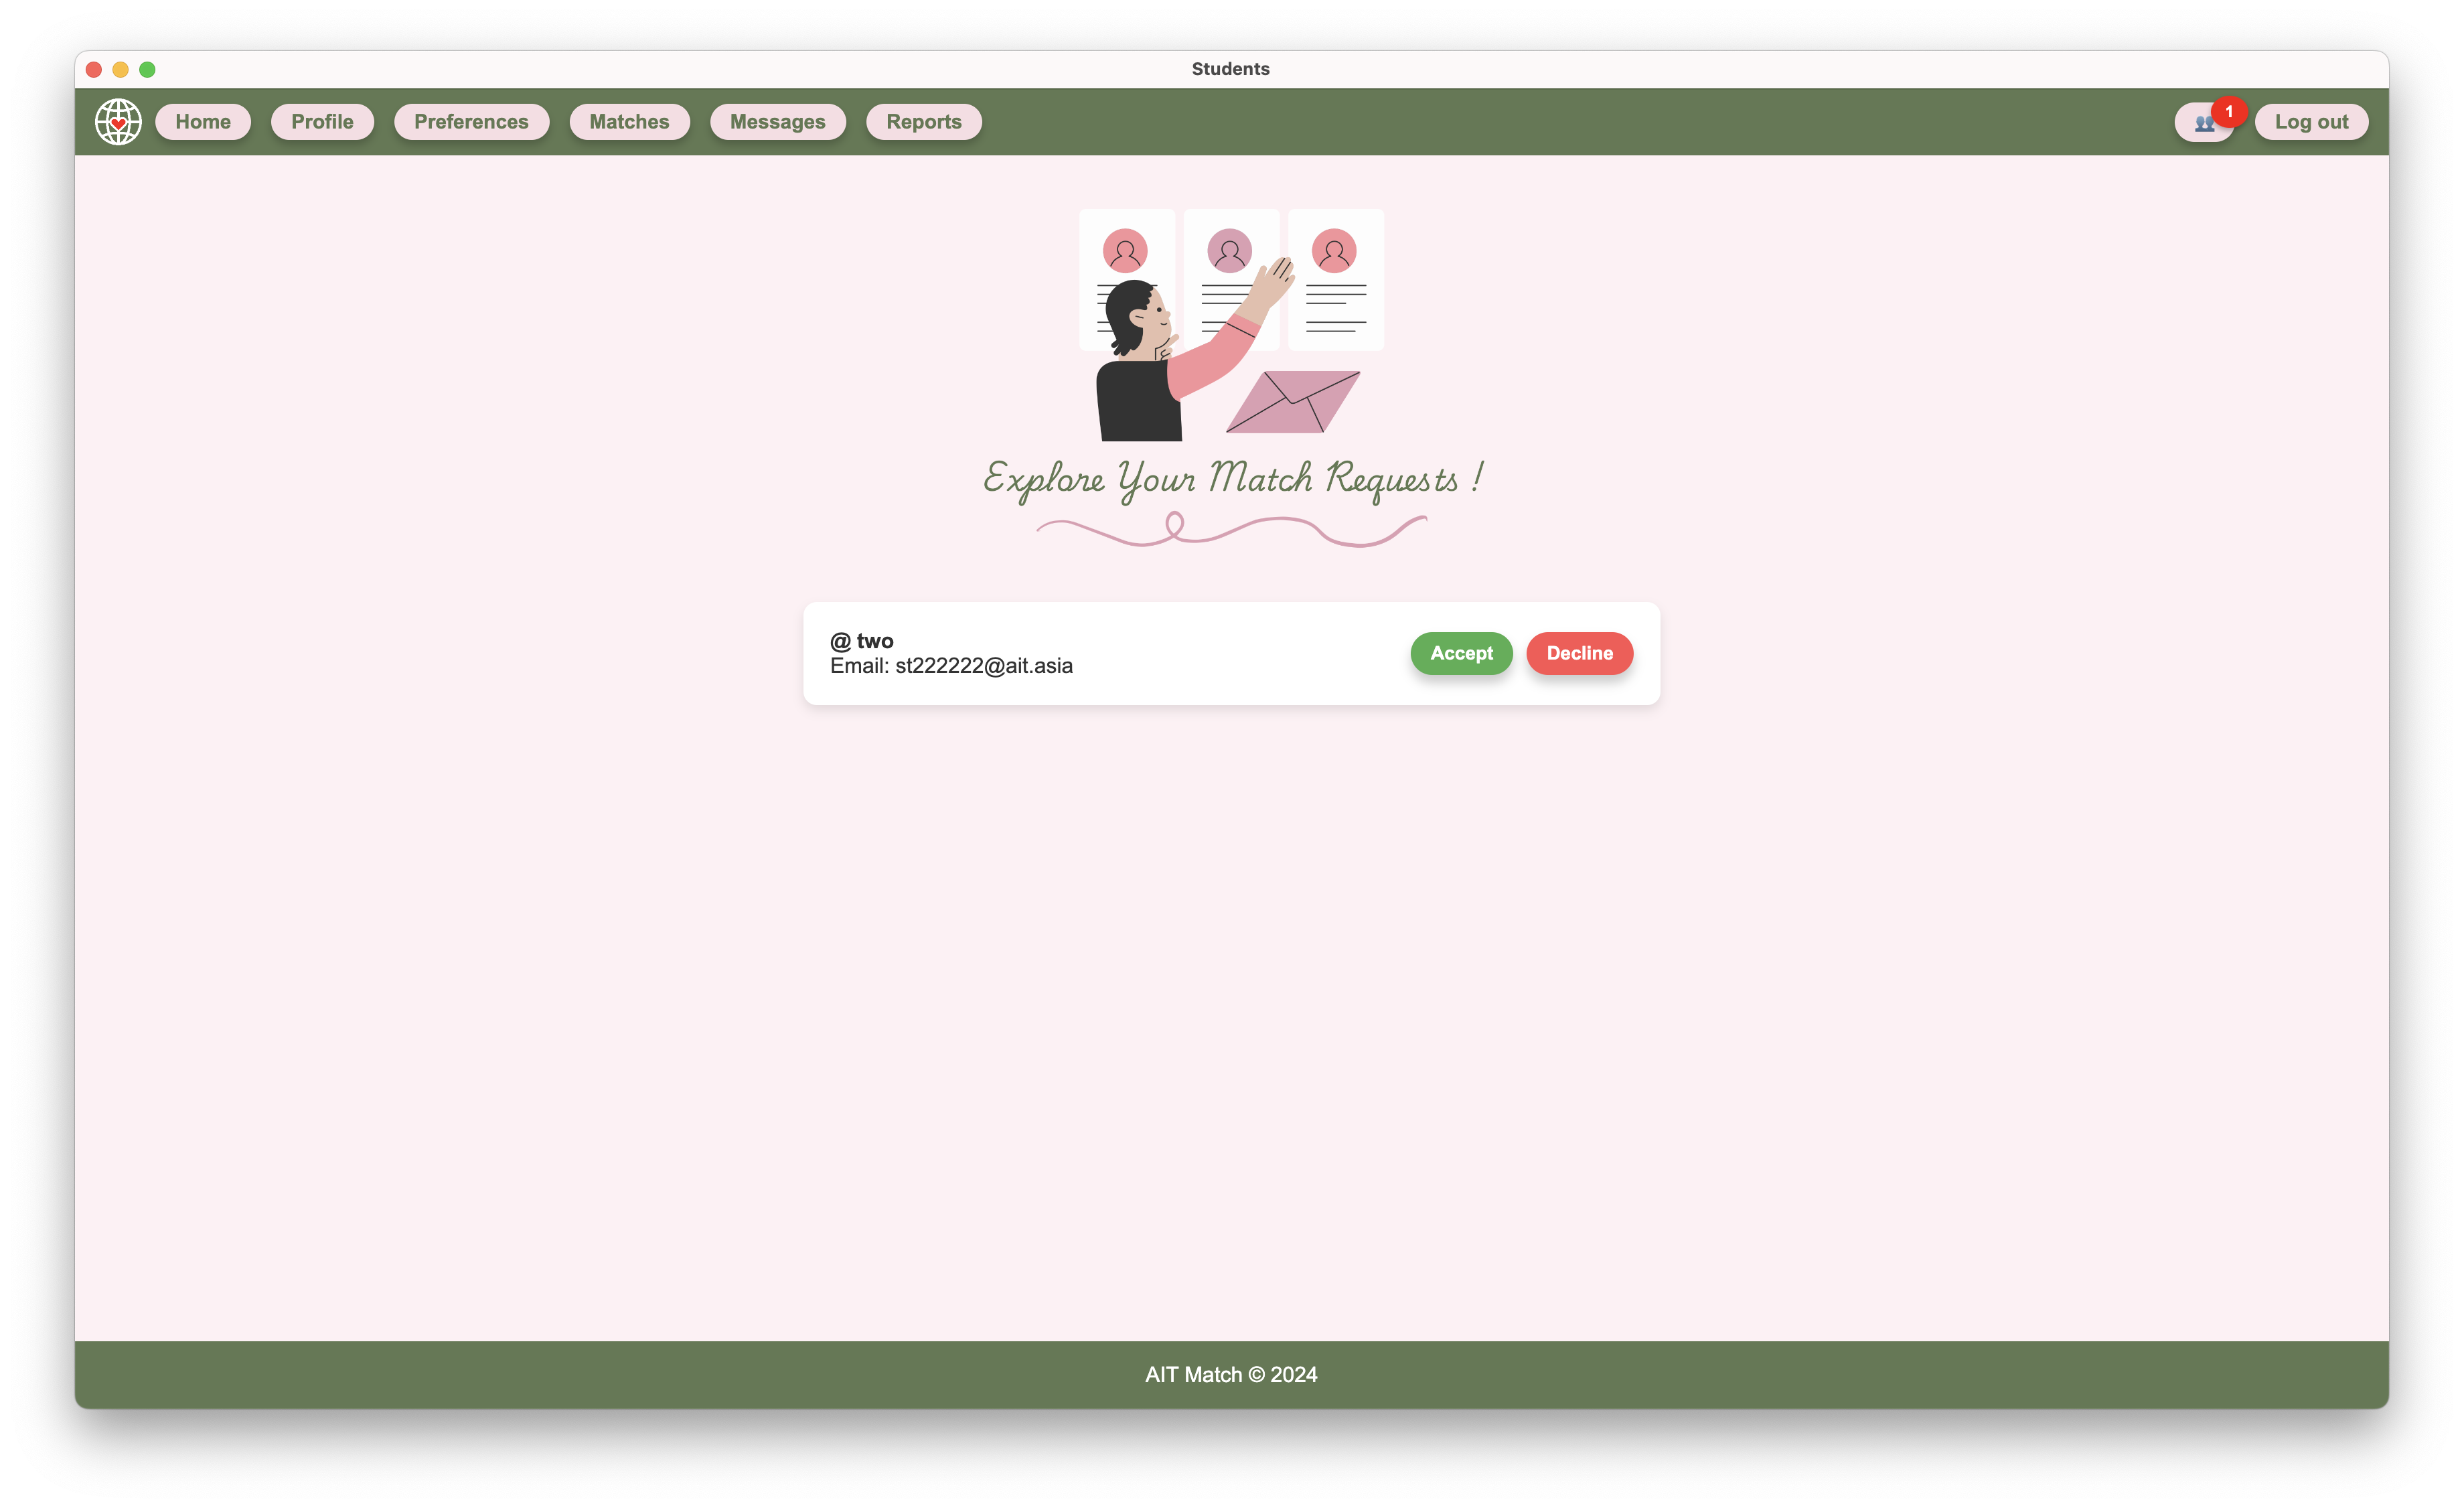
\includegraphics[width=5in]{figures/results/matches/match-request-page.png} 
                \caption{Match Requests Page.}
                \label{fig:match-request-page}
            \end{figure}

        \newpage
        \subsection{Match: No Matched Profiles Page}
        \begin{figure}[h]
                \centering
                \captionsetup{justification=centering, singlelinecheck=false, labelsep=space}
                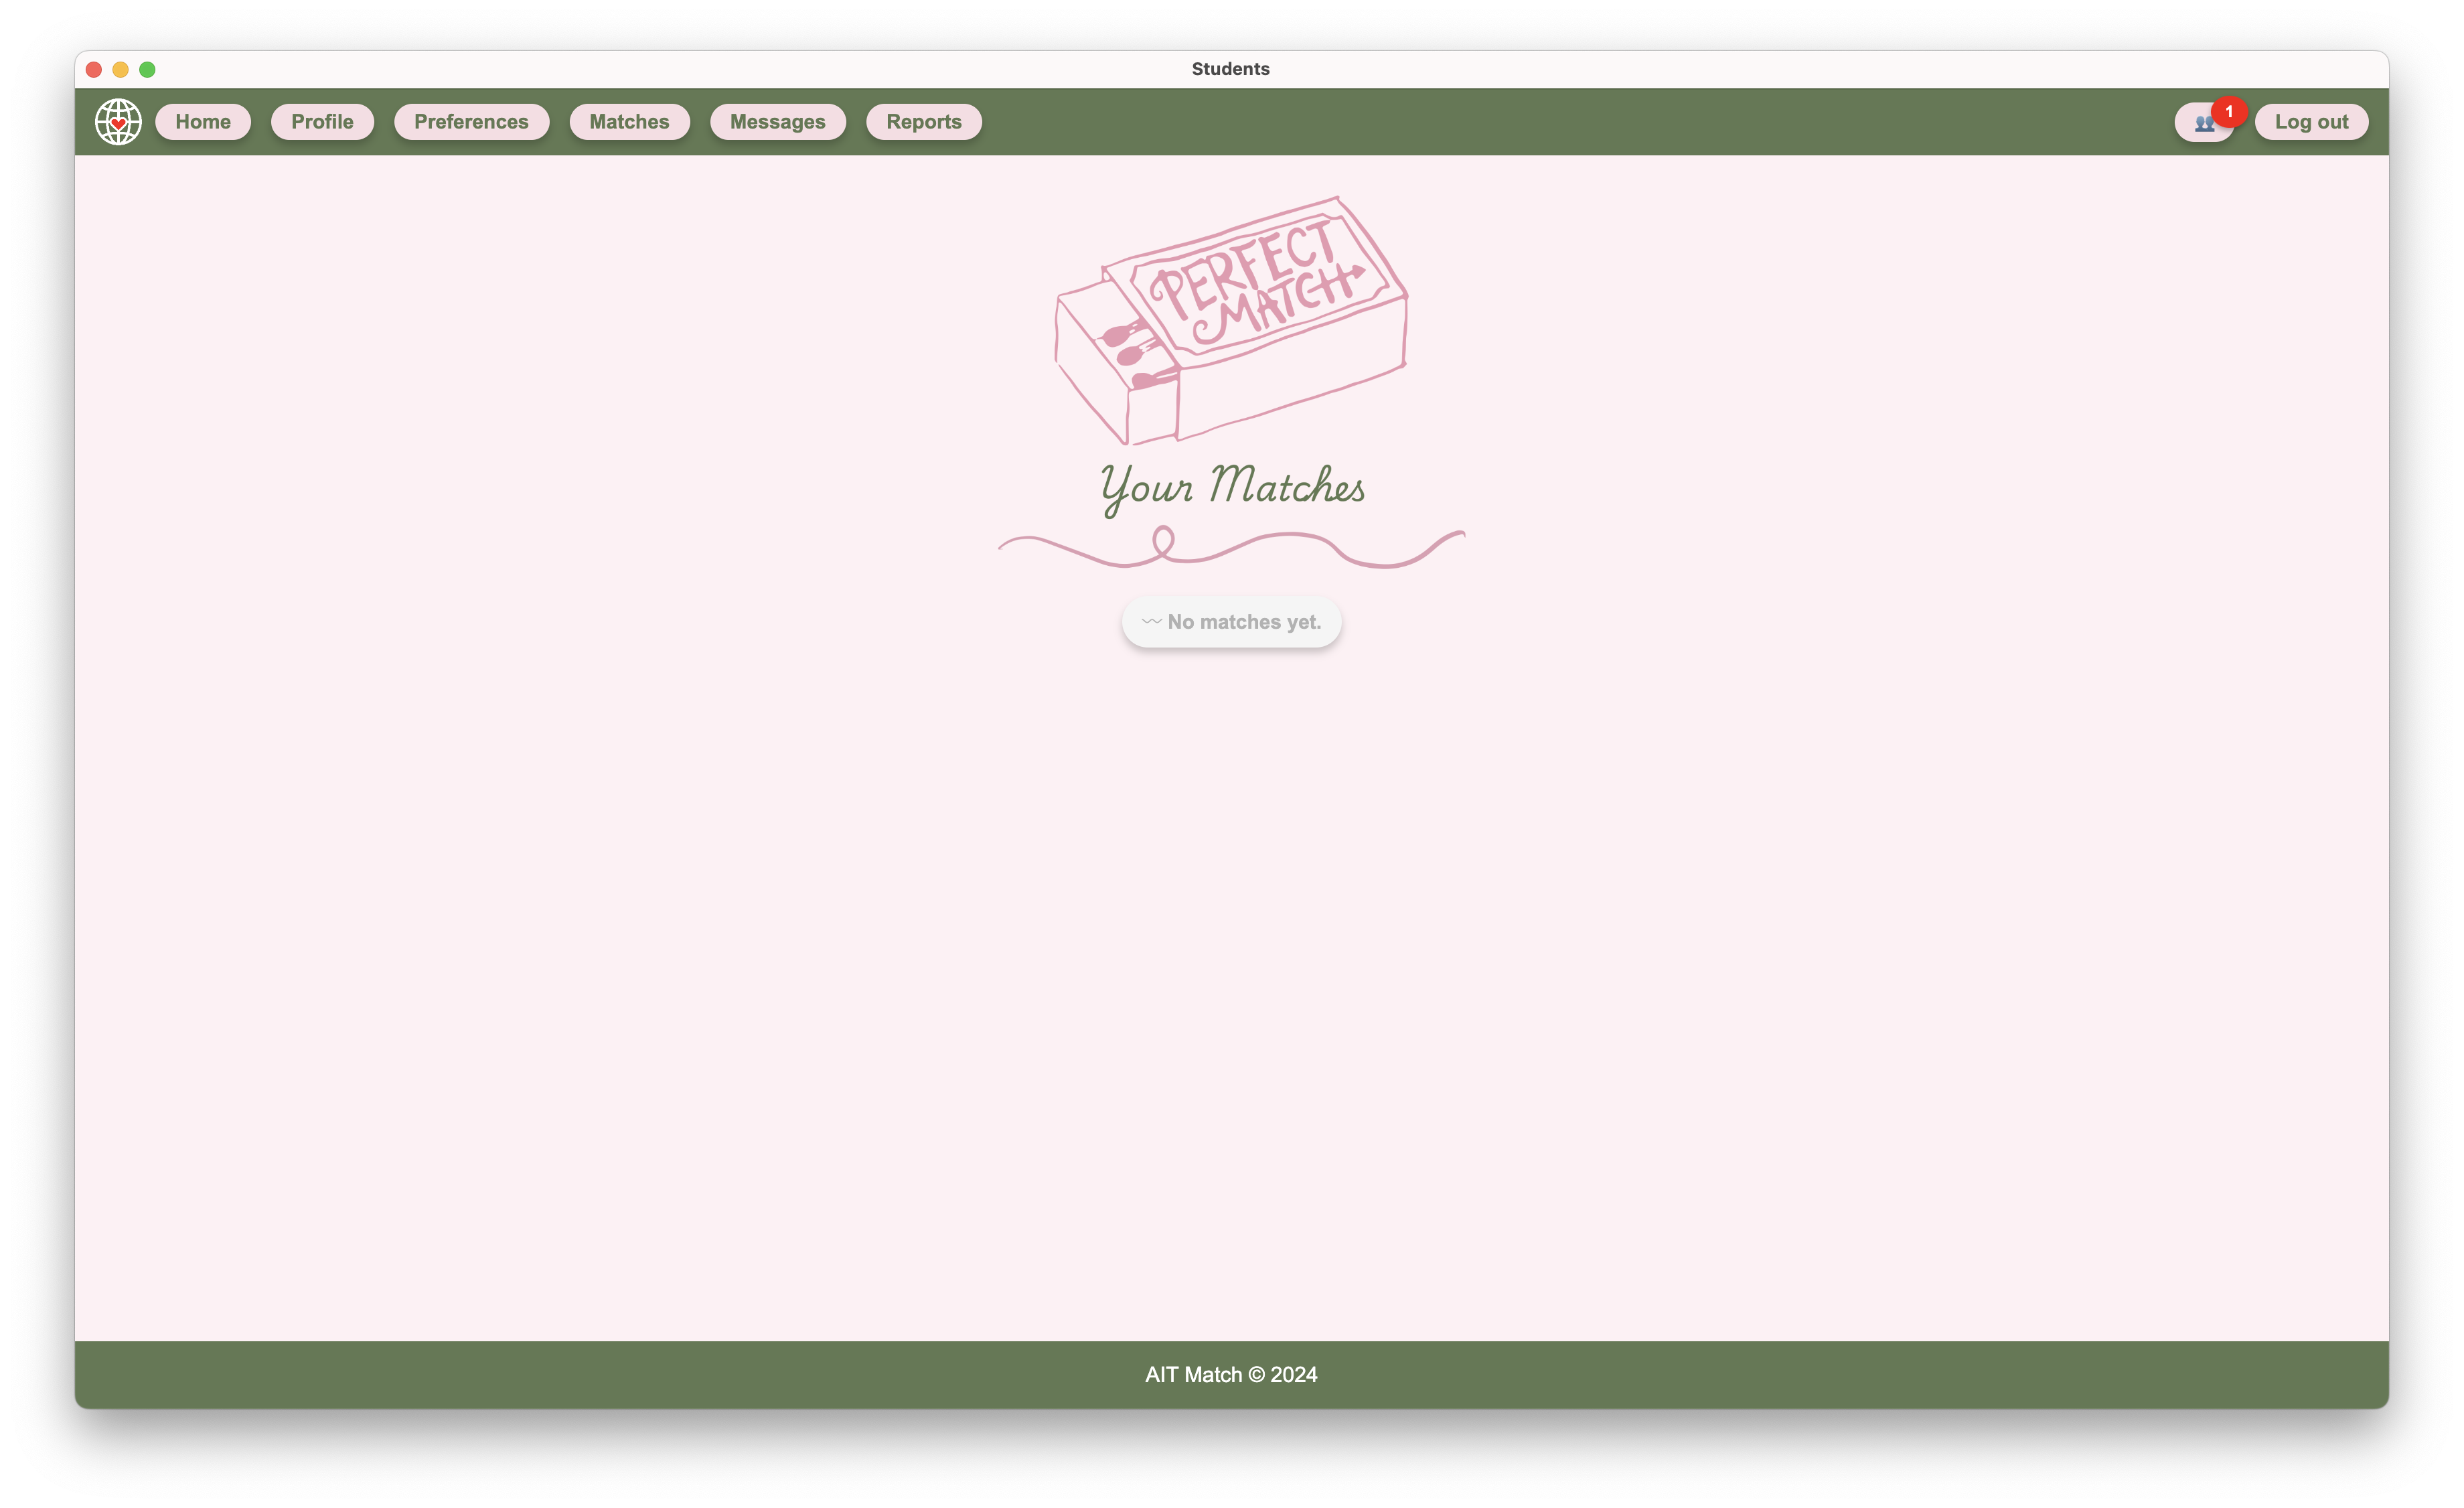
\includegraphics[width=5in]{figures/results/matches/no-matched-profile-page.png} 
                \caption{No Matched Profiles Page.}
                \label{fig:no-matched-profile-page}
            \end{figure}

        \subsection{Match: Matched Profiles Page}
        \begin{figure}[h]
                \centering
                \captionsetup{justification=centering, singlelinecheck=false, labelsep=space}
                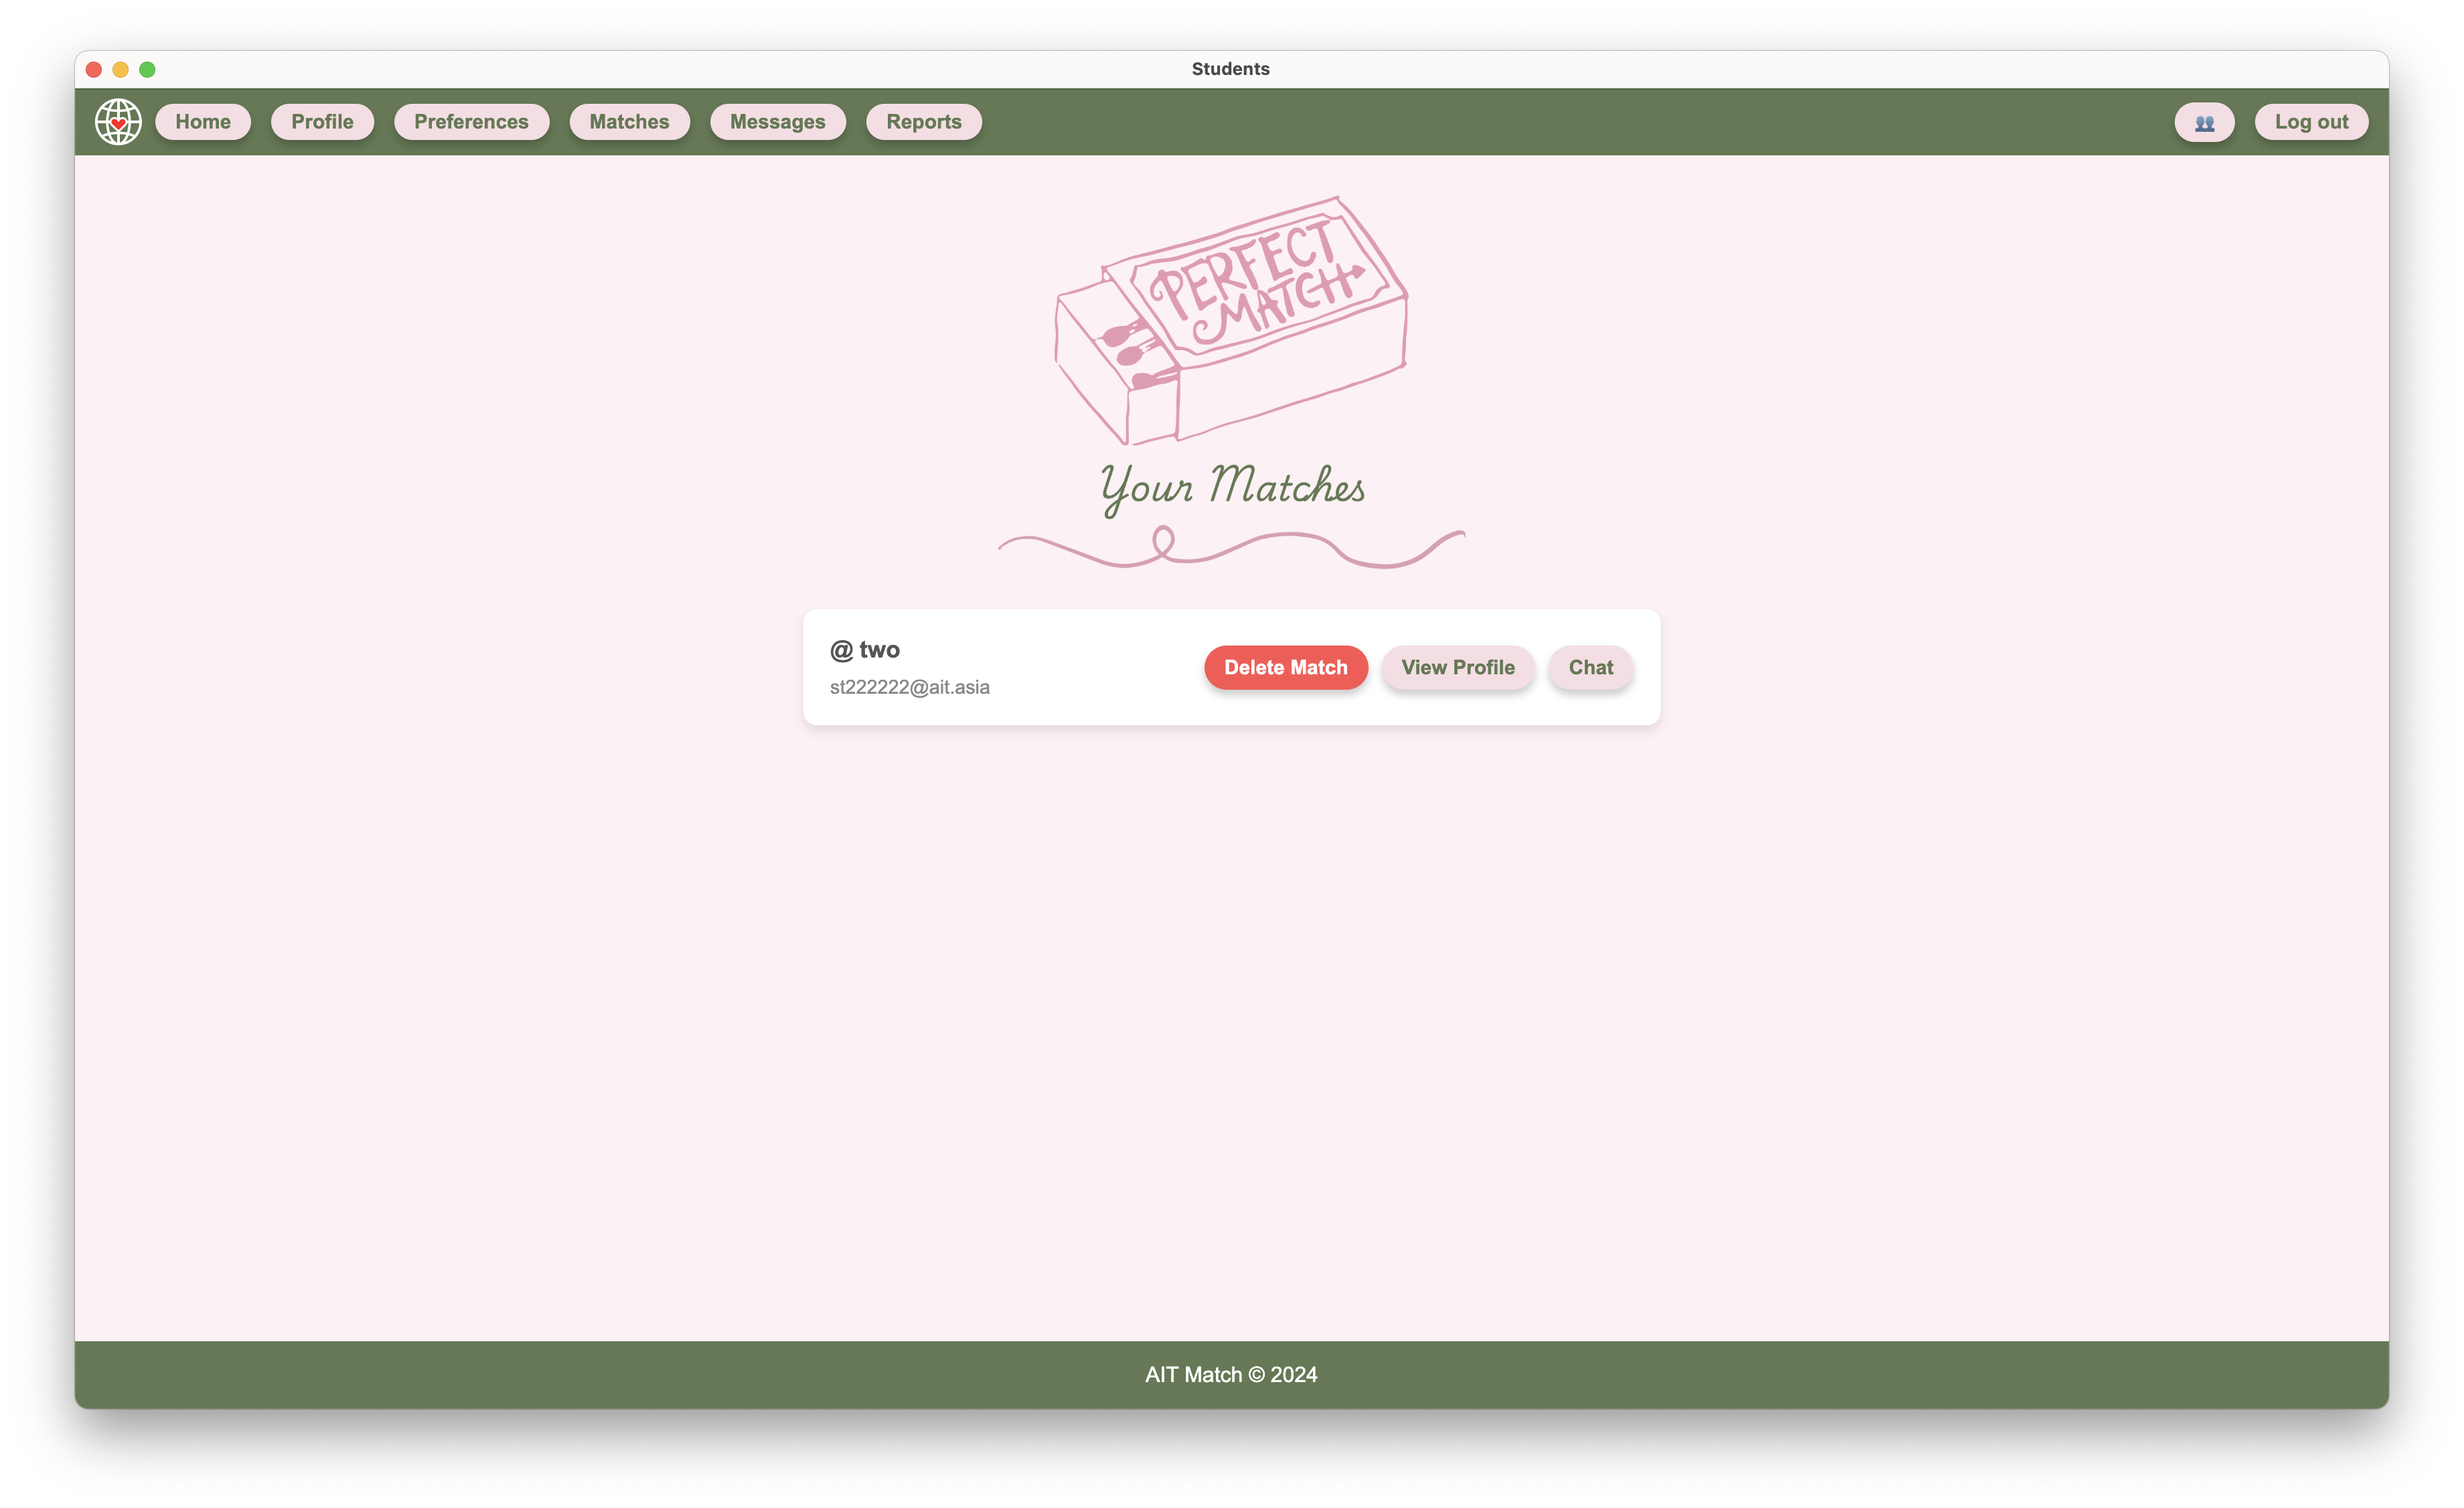
\includegraphics[width=5in]{figures/results/matches/matched-profile-page.png} 
                \caption{Matched Profiles Page.}
                \label{fig:matched-profile-page}
            \end{figure}
% ------------------------------------------------- %
        \newpage
        \subsection{Conversation: No Conversations Page}
        \begin{figure}[h]
                \centering
                \captionsetup{justification=centering, singlelinecheck=false, labelsep=space}
                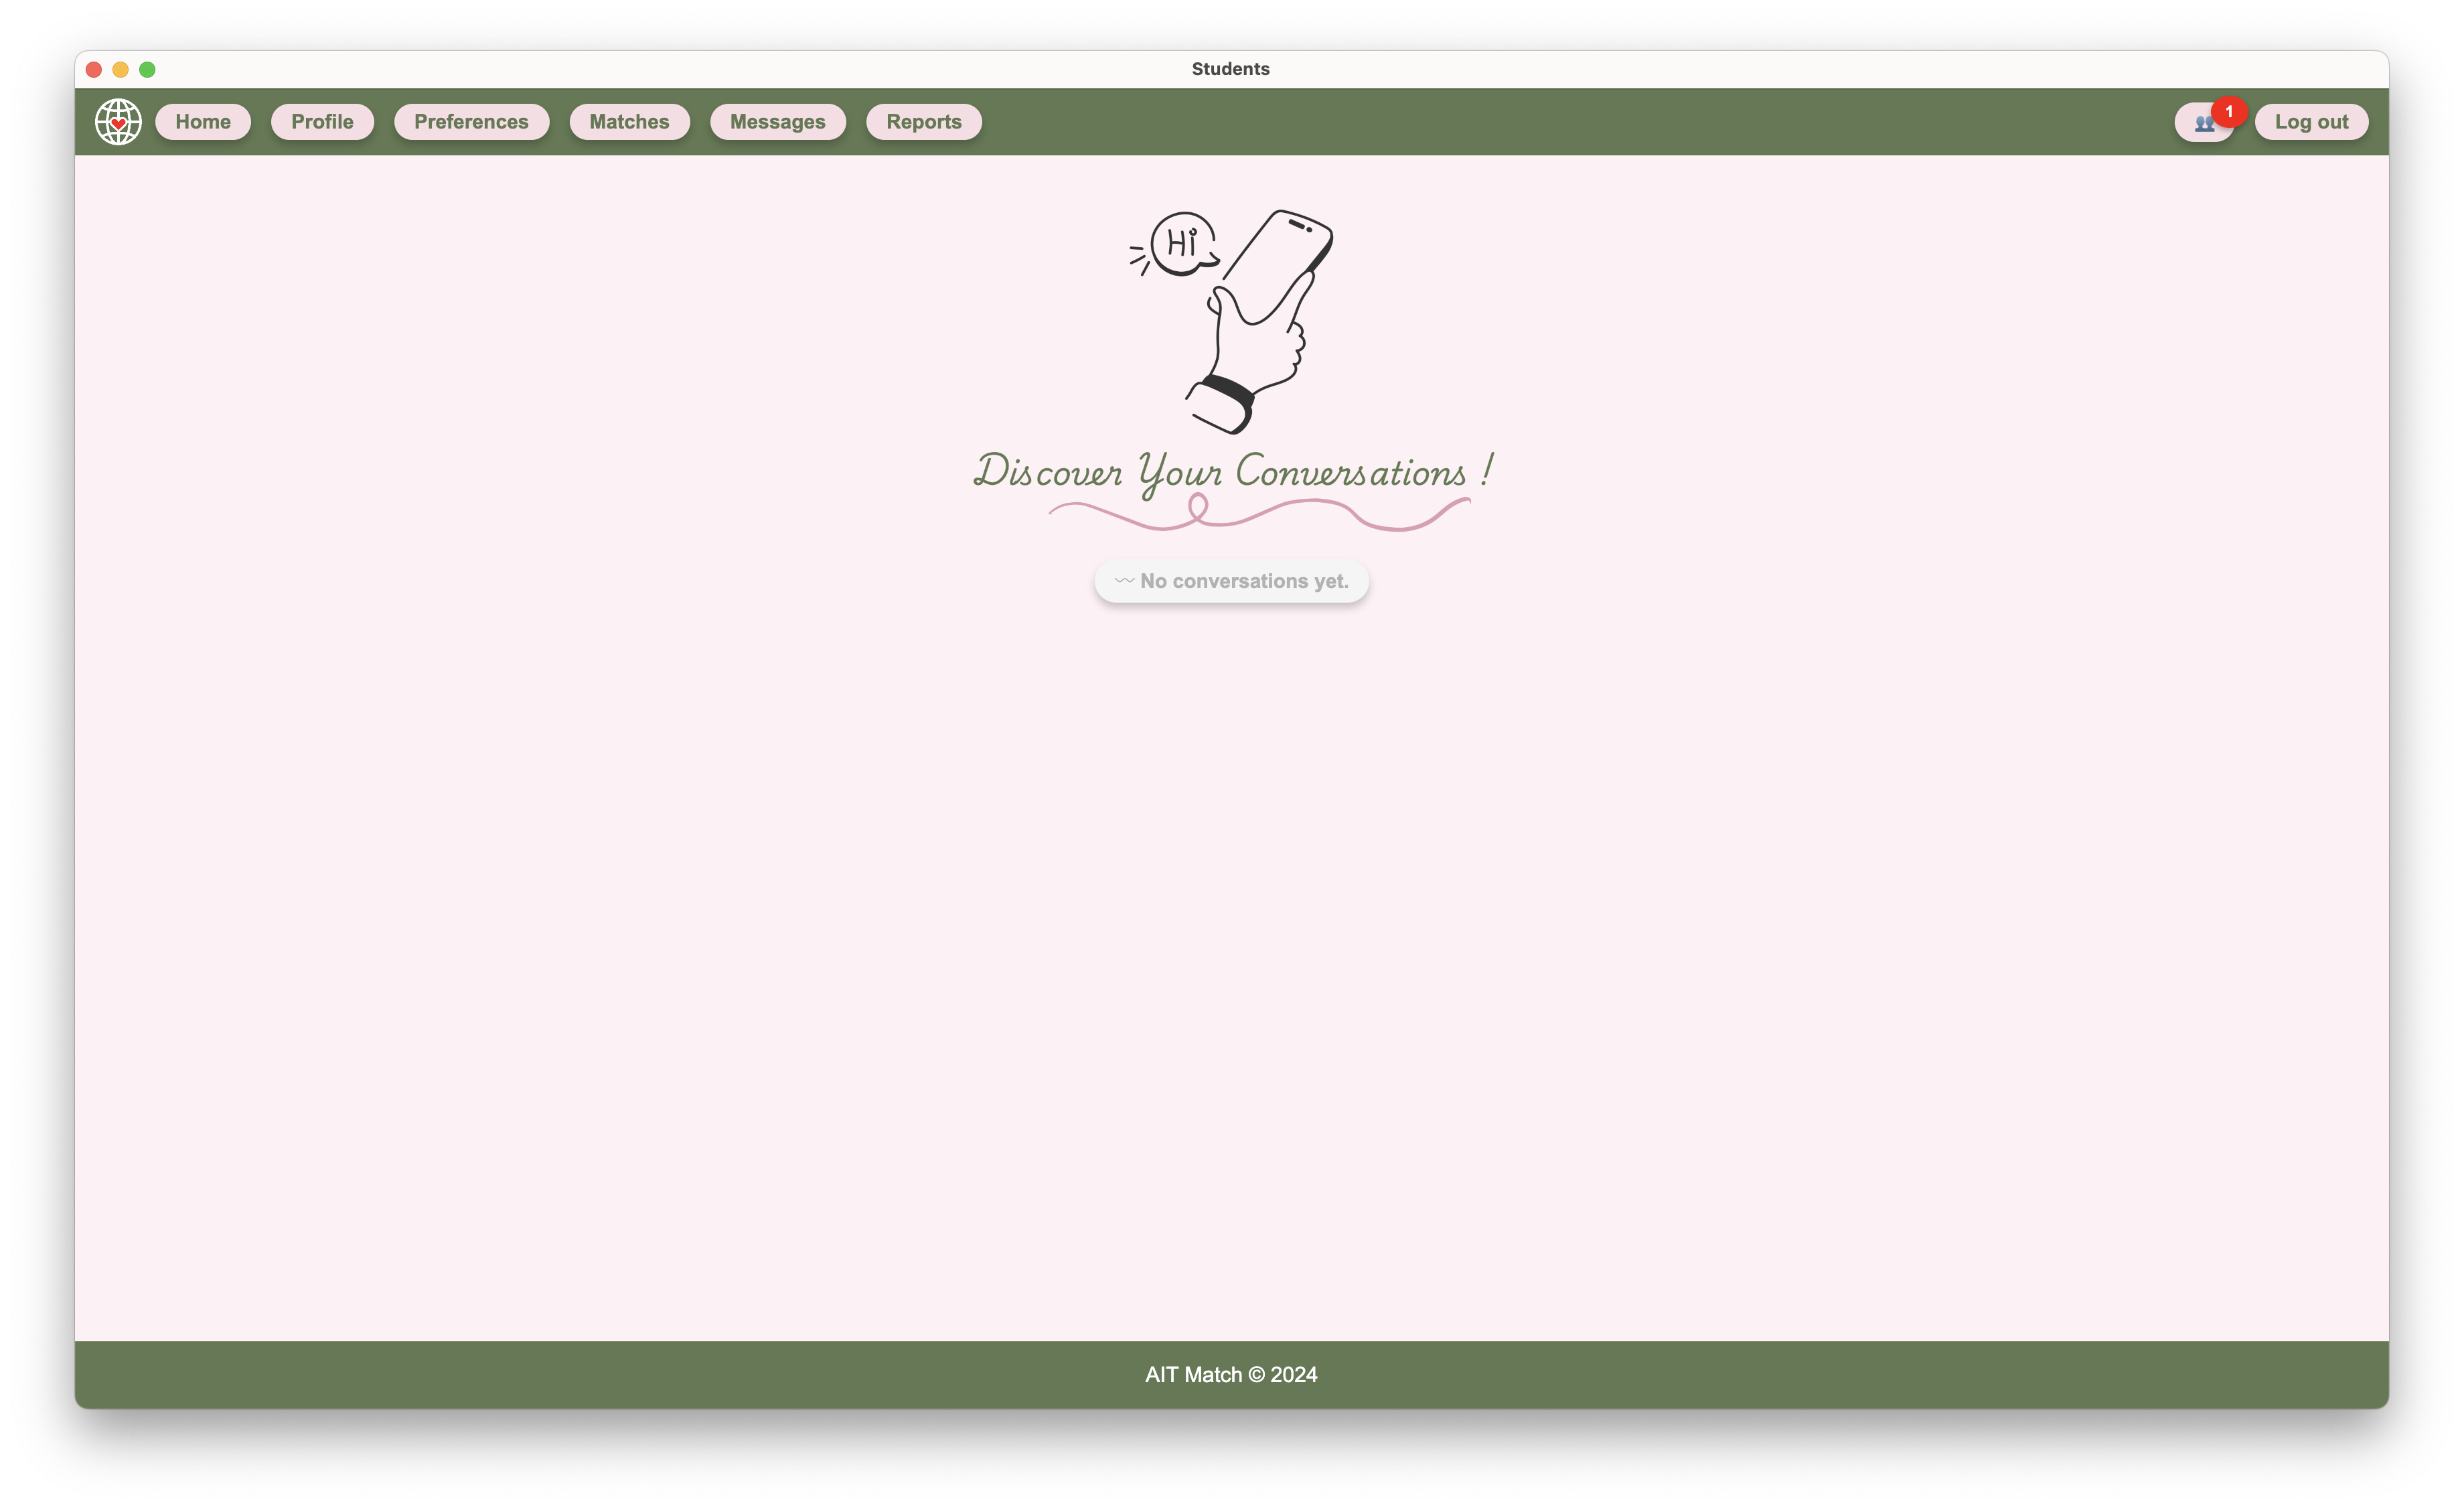
\includegraphics[width=5in]{figures/results/conversations/no-conversation-page.png} 
                \caption{No Conversations Page.}
                \label{fig:no-conversation-page.png}
            \end{figure}

        \subsection{Conversation: Conversations Page}
        \begin{figure}[h]
                \centering
                \captionsetup{justification=centering, singlelinecheck=false, labelsep=space}
                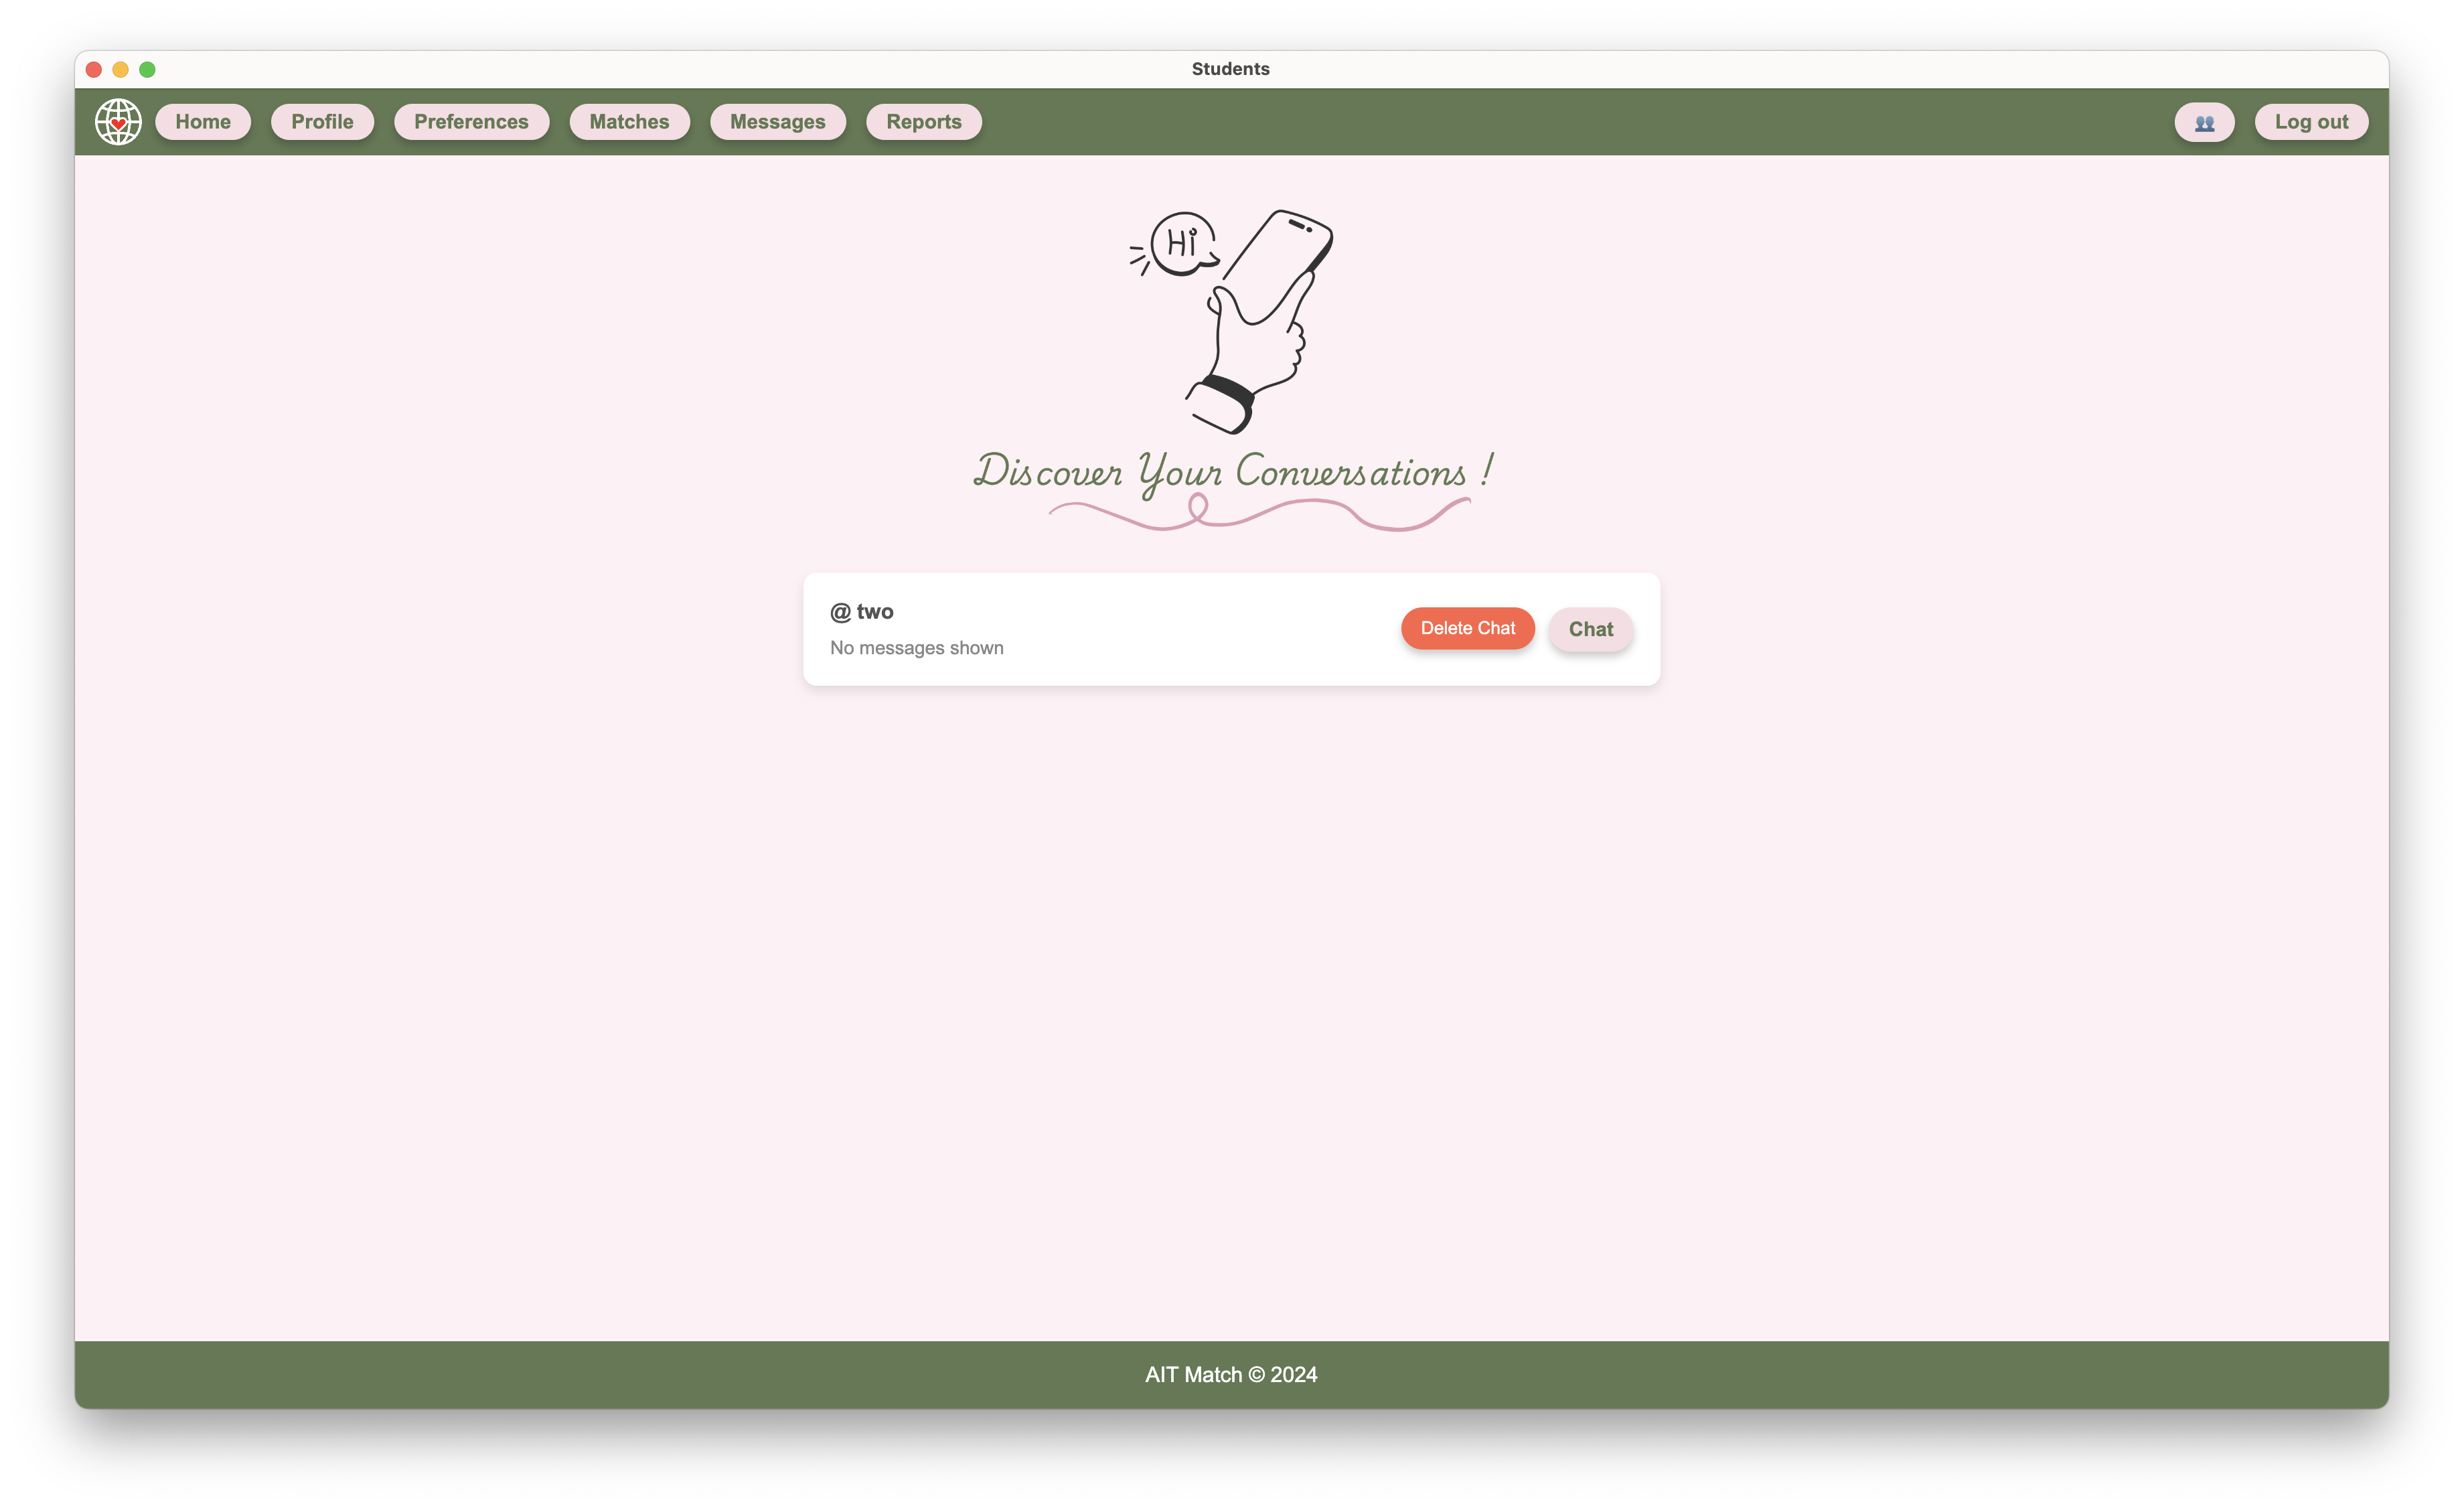
\includegraphics[width=5in]{figures/results/conversations/conversation-page.png} 
                \caption{Conversations Page.}
                \label{fig:conversation-page.png}
            \end{figure}
% ------------------------------------------------- %
        \newpage
        \subsection{Chat: Chat Room Page}
        \begin{figure}[h]
                \centering
                \captionsetup{justification=centering, singlelinecheck=false, labelsep=space}
                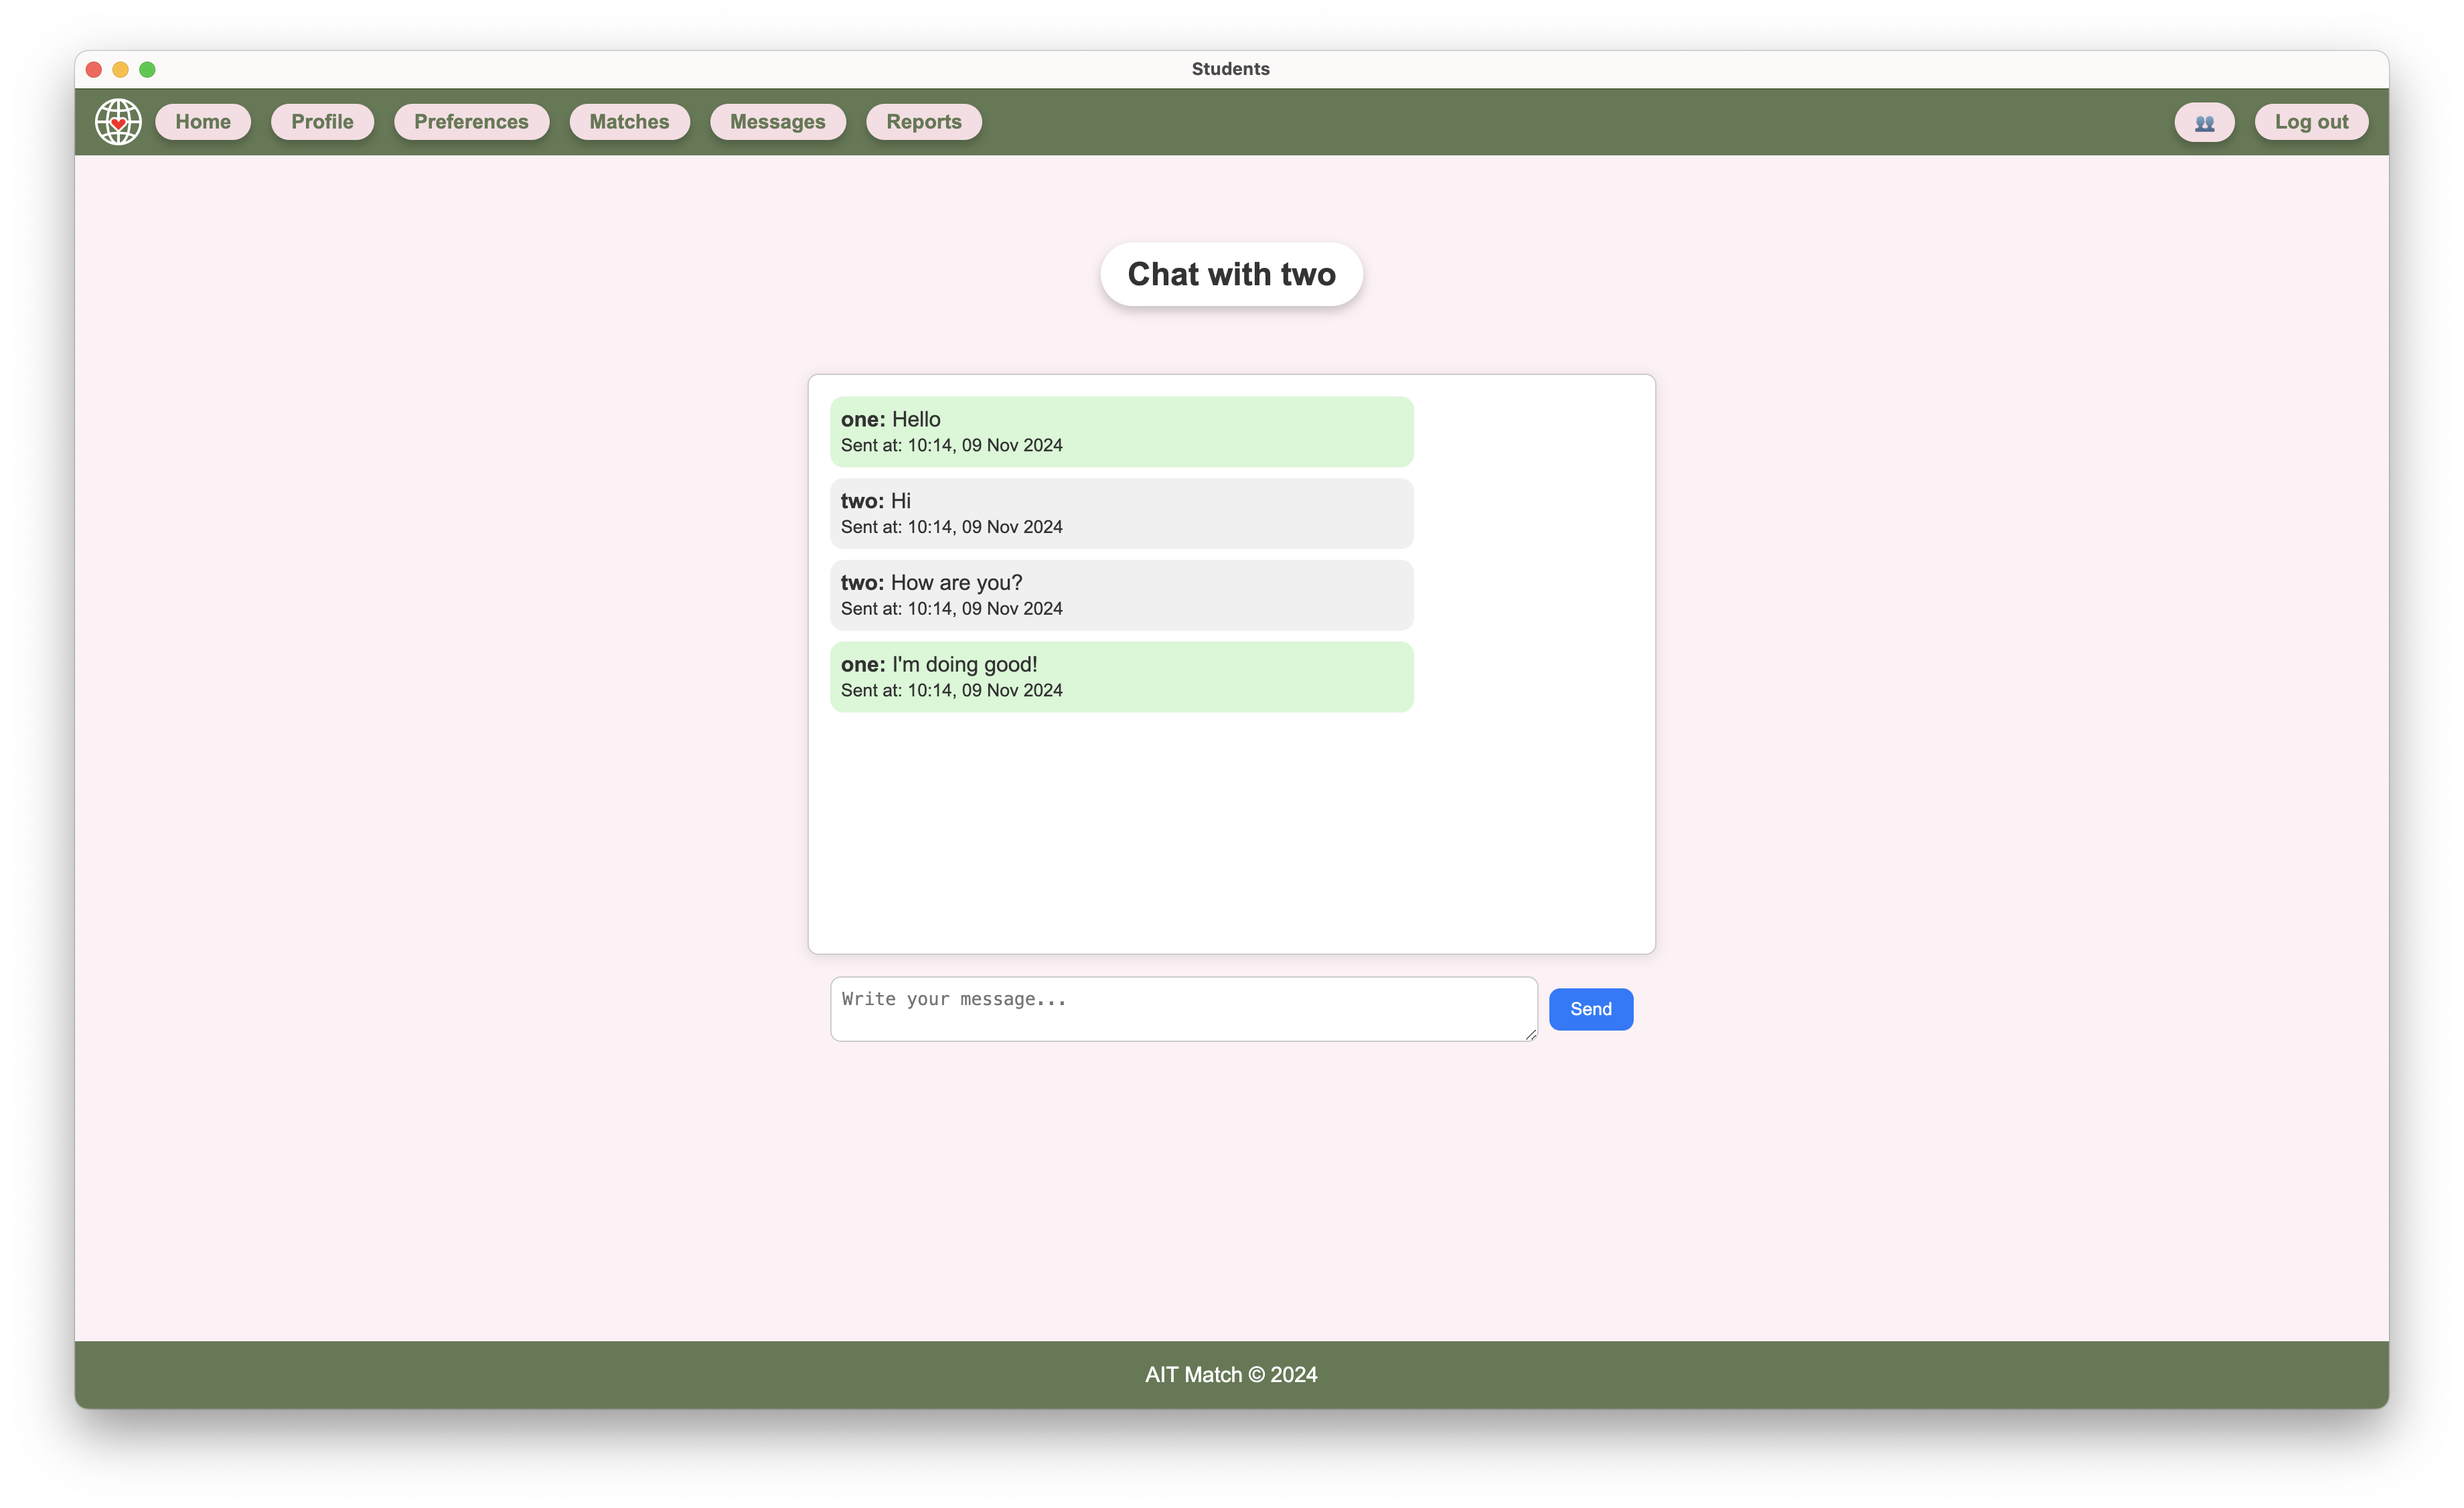
\includegraphics[width=5in]{figures/results/chat/chat-room-page.png} 
                \caption{Chat Room Page.}
                \label{fig:no-conversation-page.png}
            \end{figure}
% ------------------------------------------------- %
        \newpage
        \subsection{Report: Reported Profile Page}
        \begin{figure}[h]
                \centering
                \captionsetup{justification=centering, singlelinecheck=false, labelsep=space}
                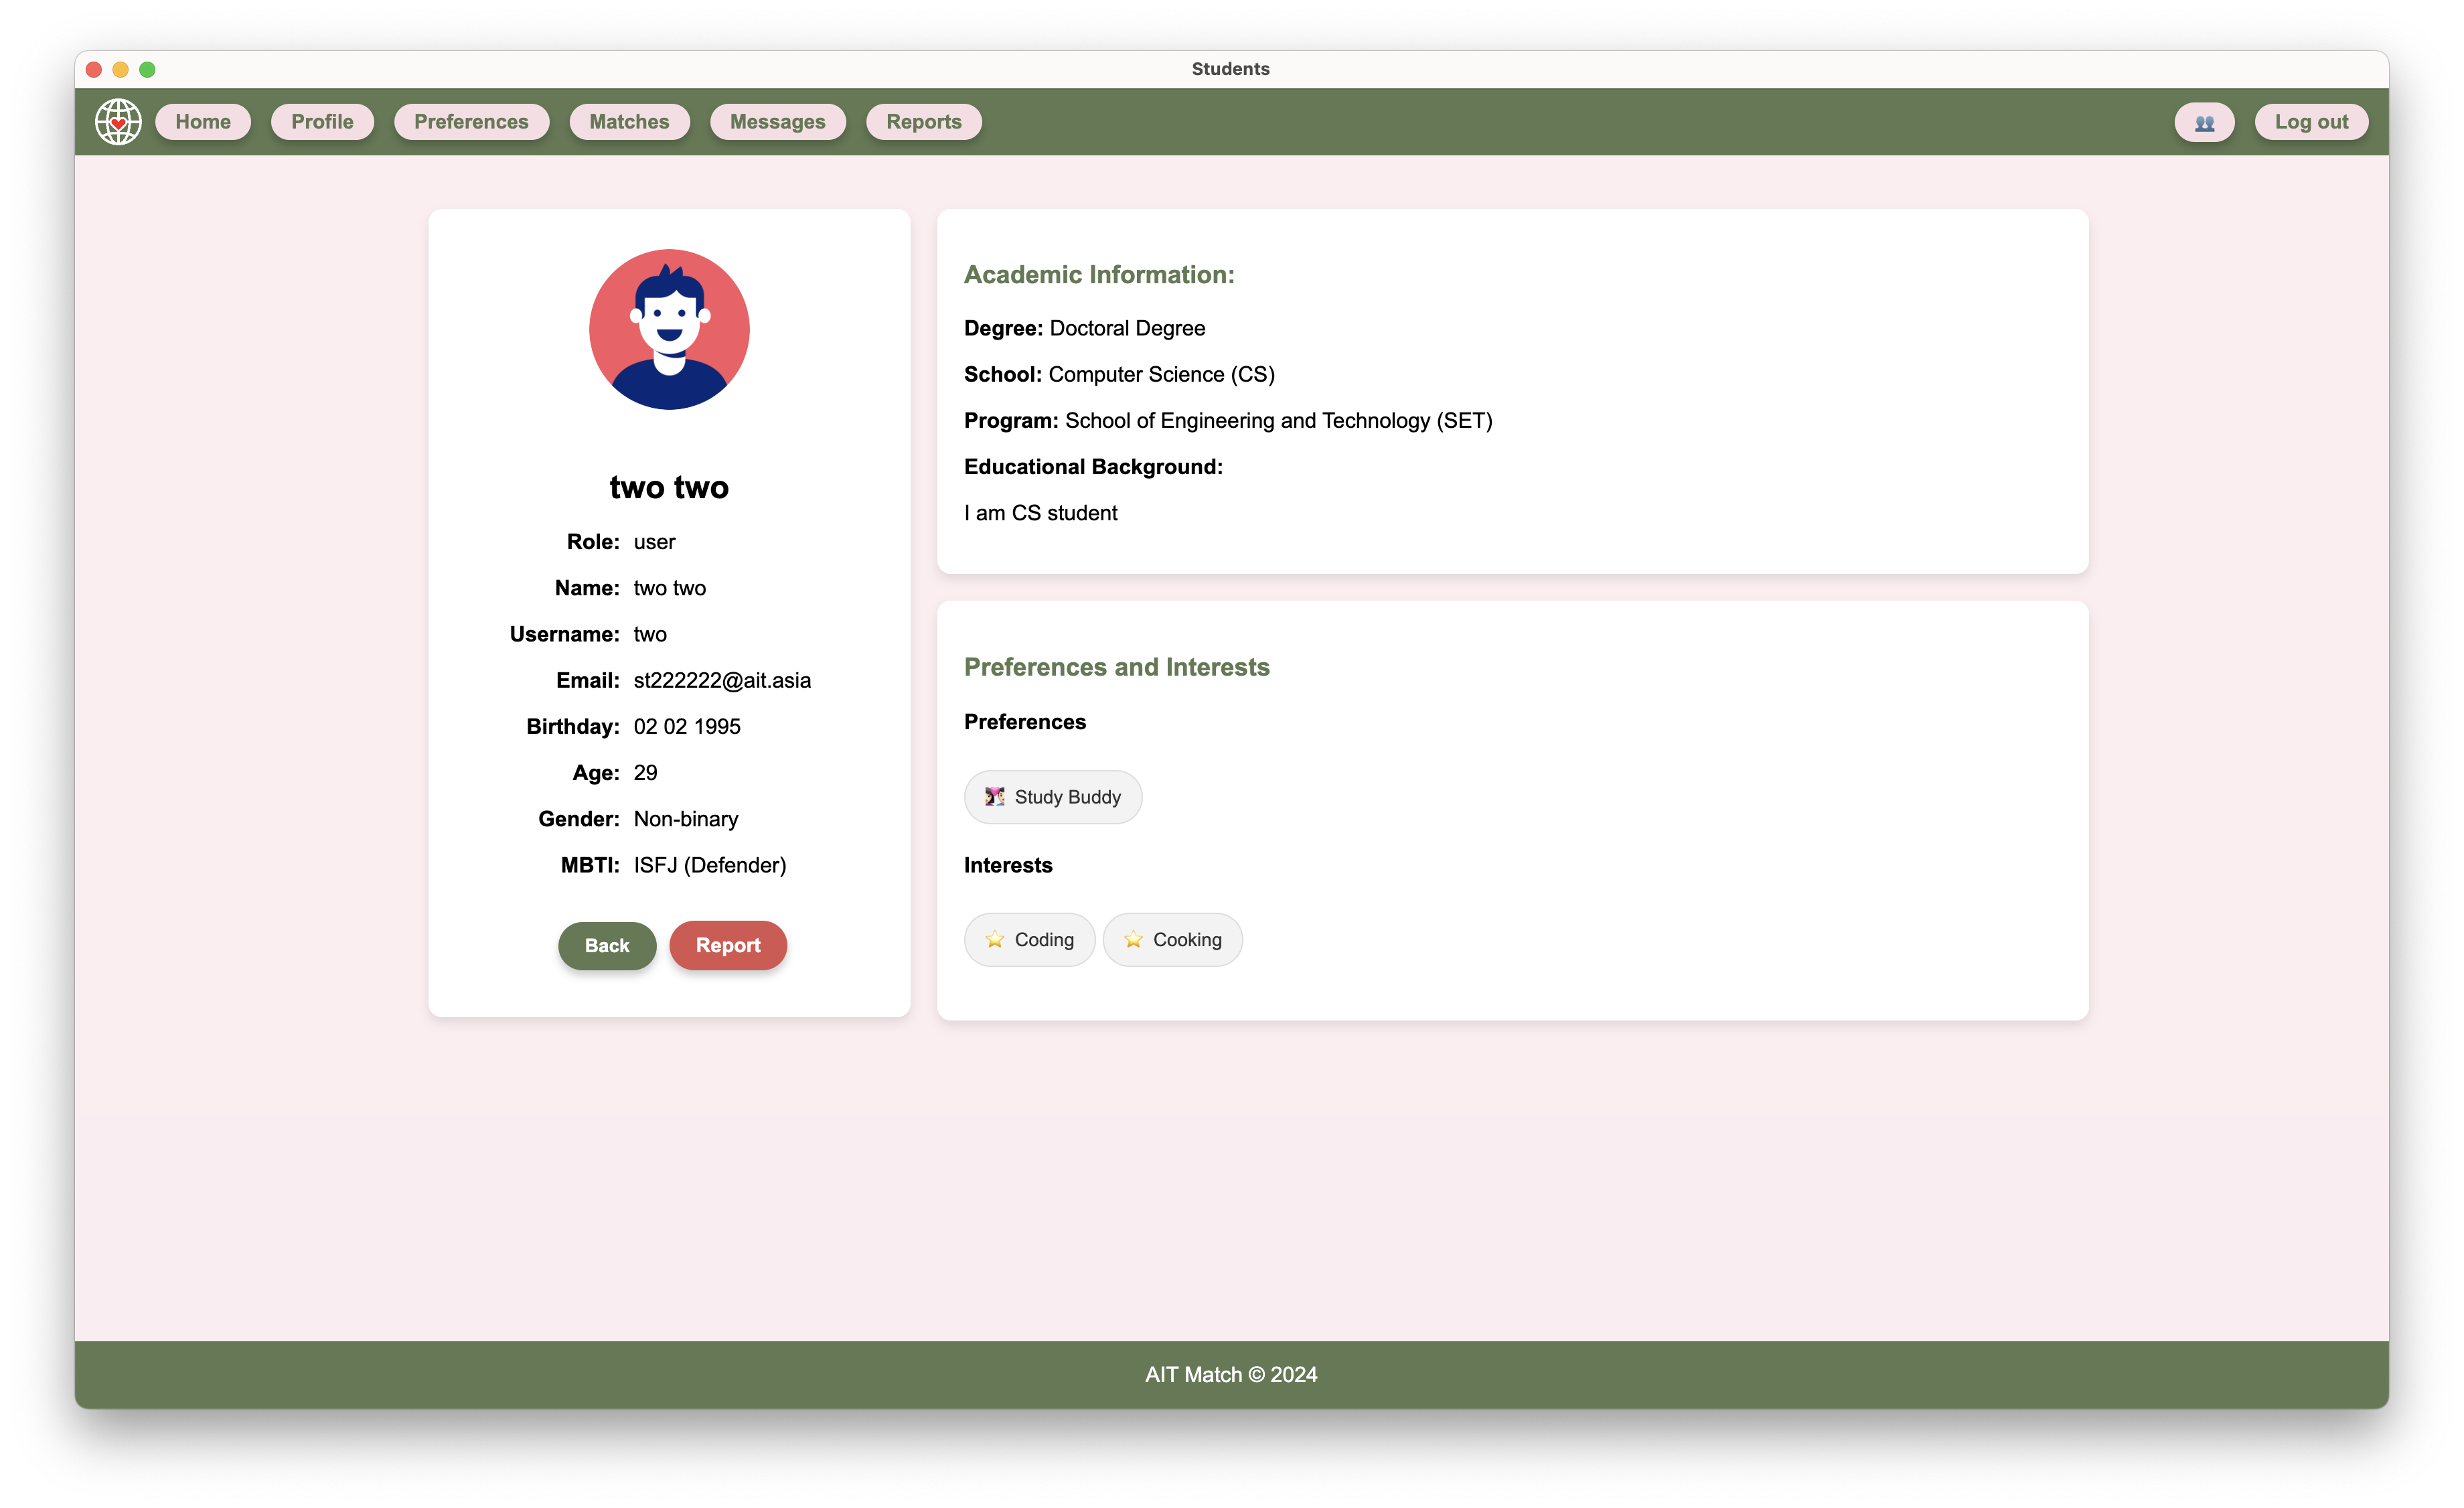
\includegraphics[width=5in]{figures/results/reports/reported-profile-page.png} 
                \caption{Reported Profile Page.}
                \label{fig:reported-profile-page}
            \end{figure}

        \subsection{Report: New Report Page}
        \begin{figure}[h]
                \centering
                \captionsetup{justification=centering, singlelinecheck=false, labelsep=space}
                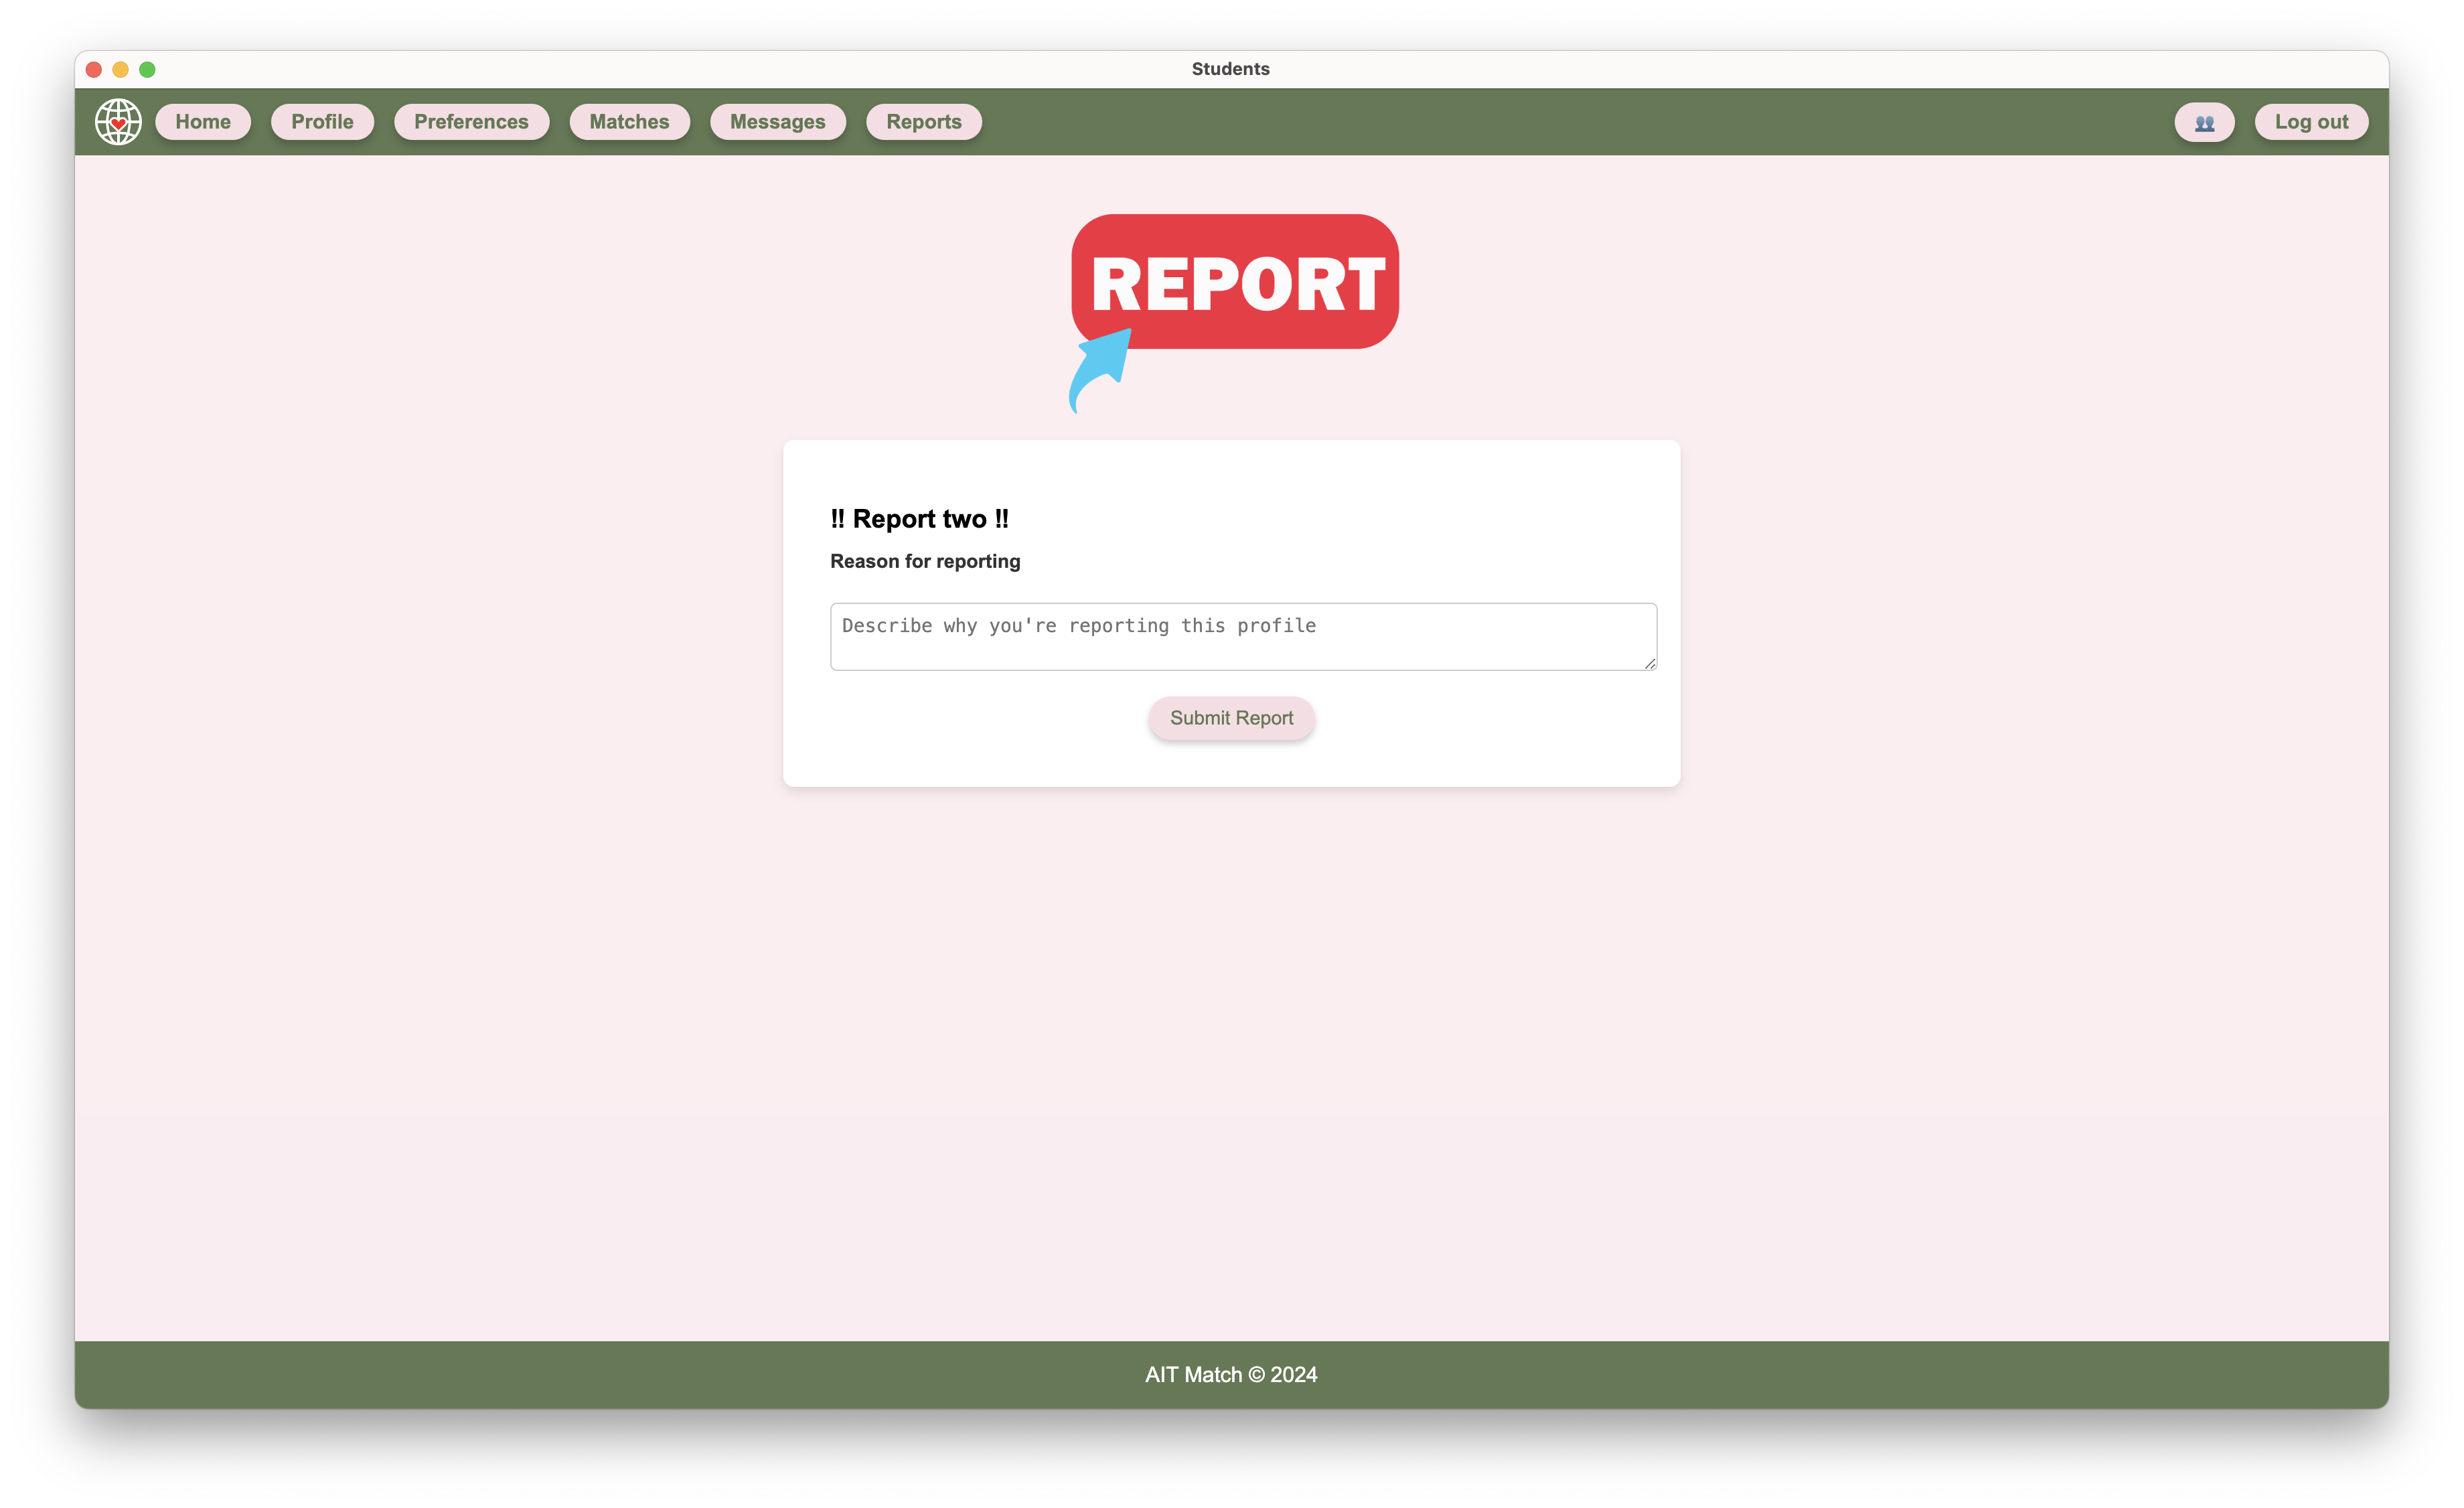
\includegraphics[width=5in]{figures/results/reports/report-new-page.png}
                \caption{New Report Page.}
                \label{fig:report-new-page}
            \end{figure}

        \newpage
        \subsection{Report: No Report Page}
        \begin{figure}[h]
                \centering
                \captionsetup{justification=centering, singlelinecheck=false, labelsep=space}
                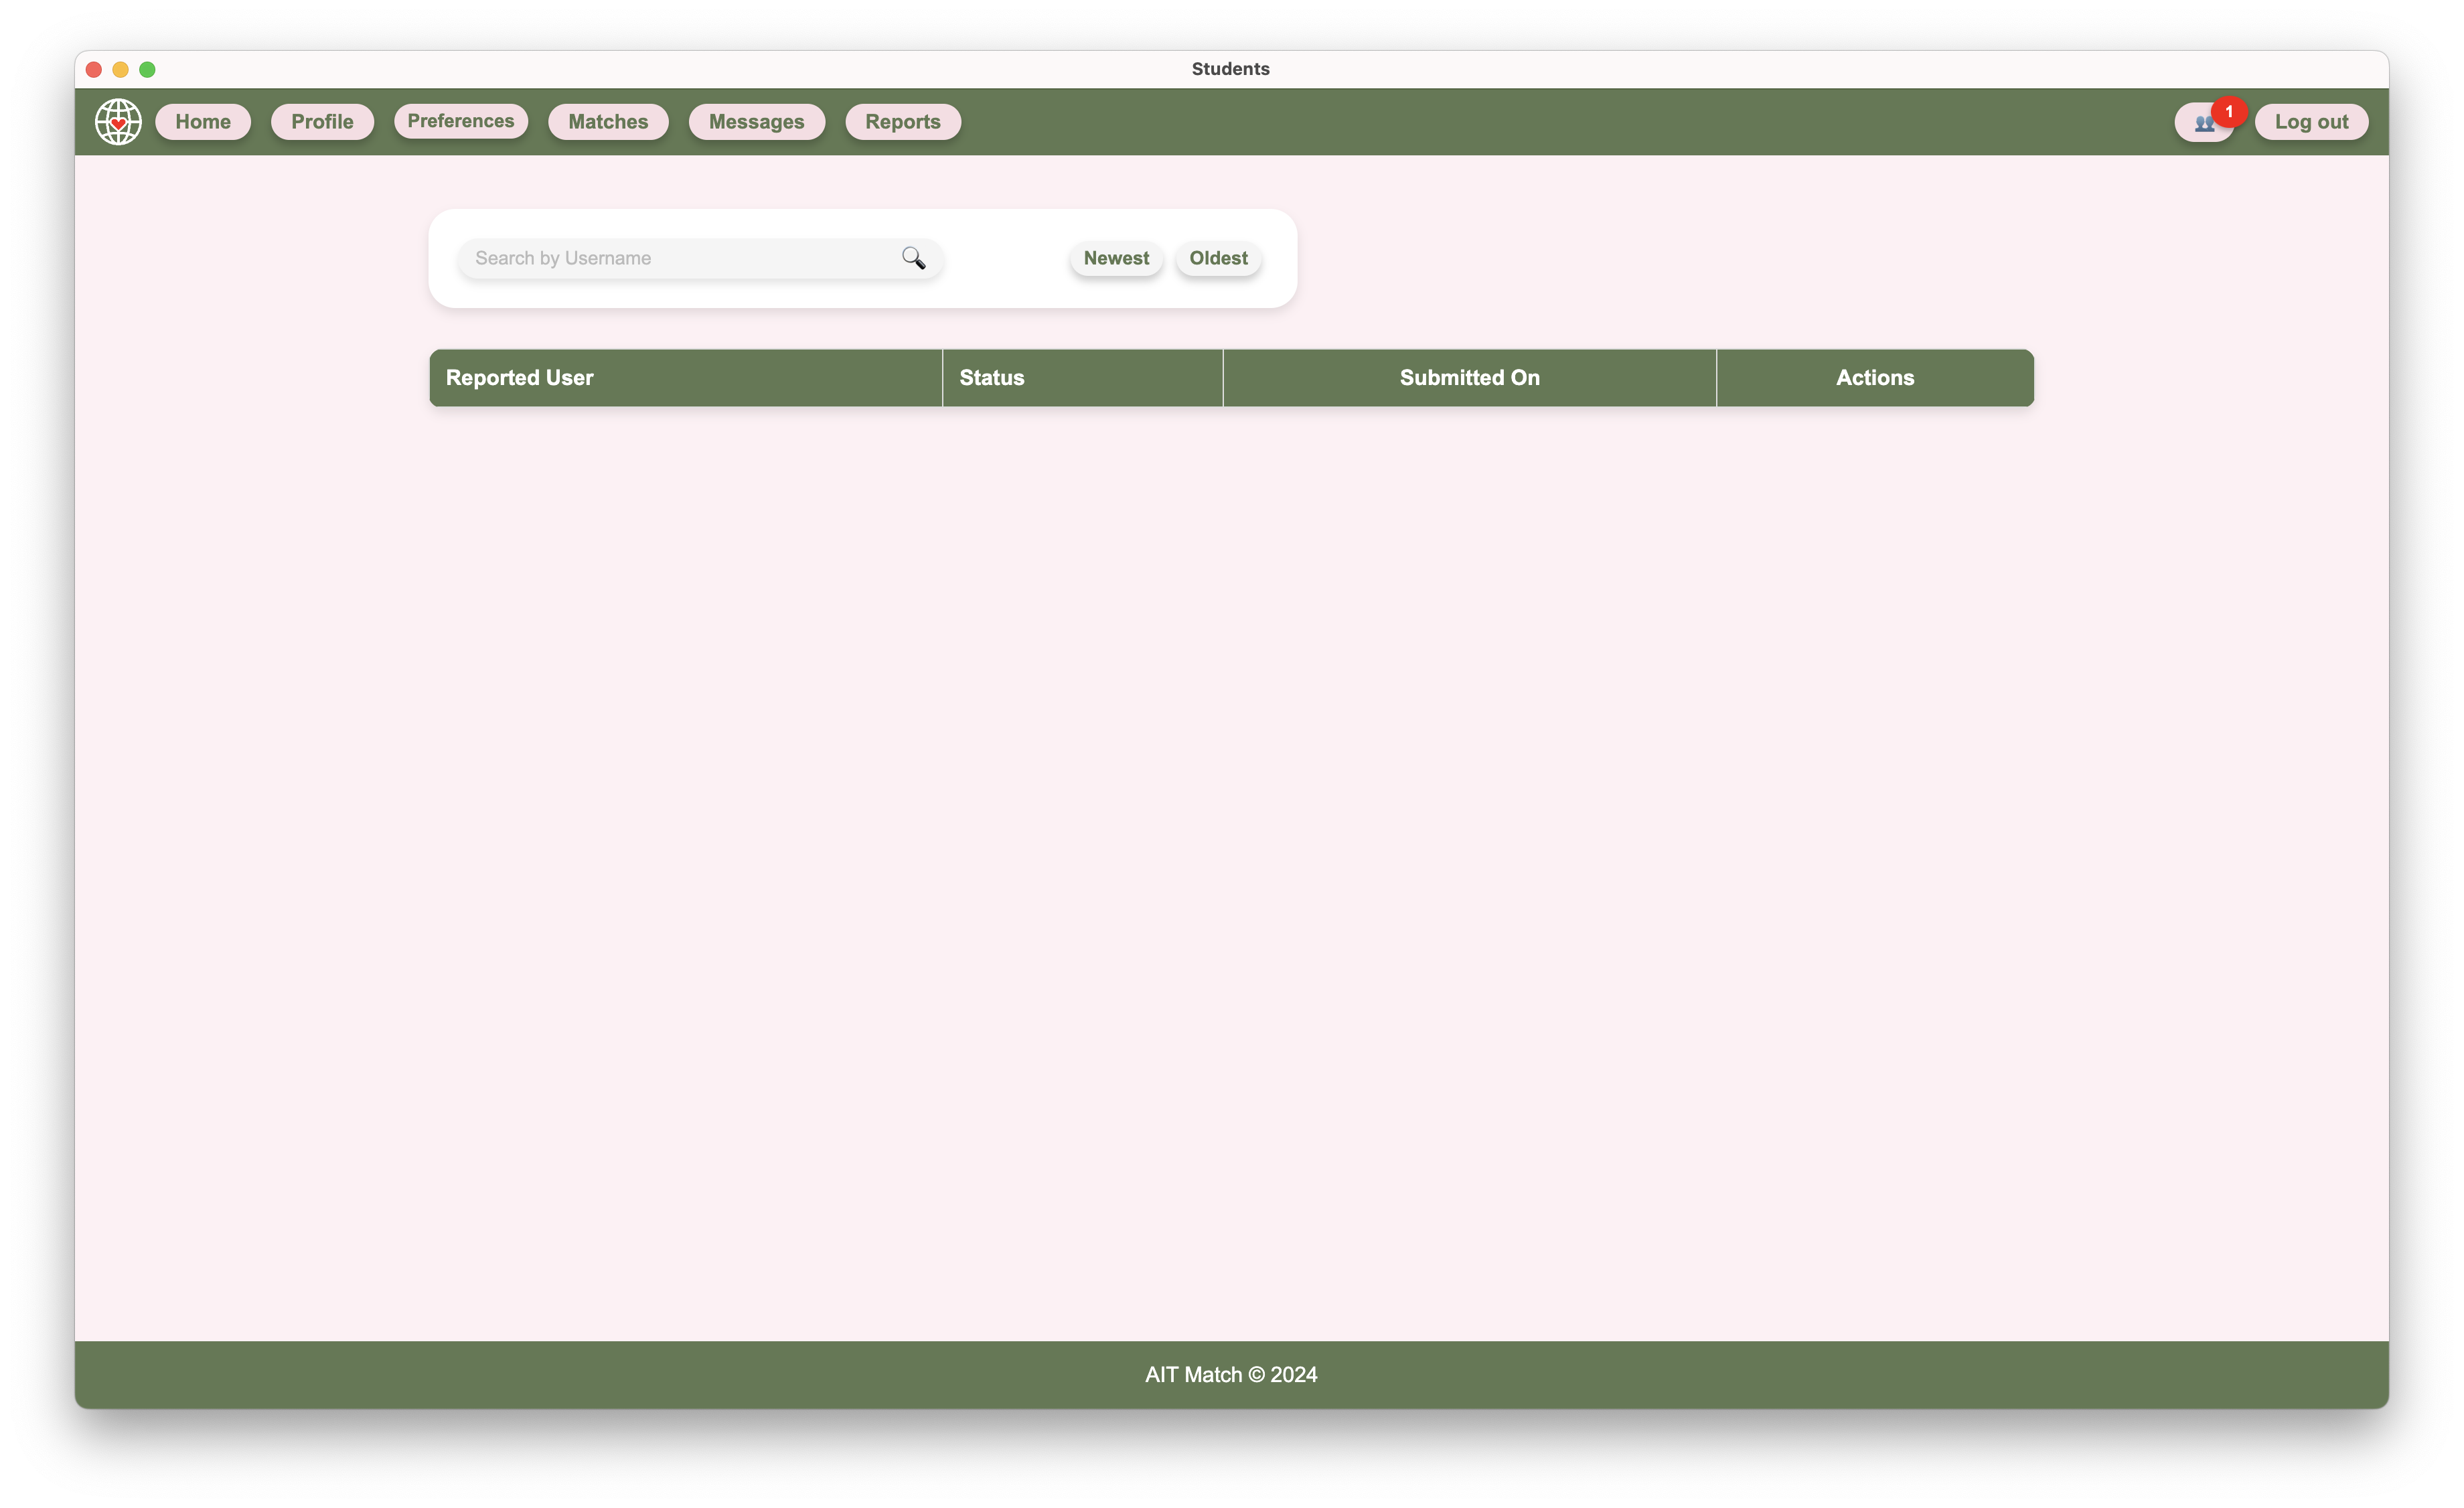
\includegraphics[width=5in]{figures/results/reports/no-reports-page.png}
                \caption{No Report Page.}
                \label{fig:no-reports-page}
            \end{figure}

        \subsection{Report: Report Index Page}
        \begin{figure}[h]
                \centering
                \captionsetup{justification=centering, singlelinecheck=false, labelsep=space}
                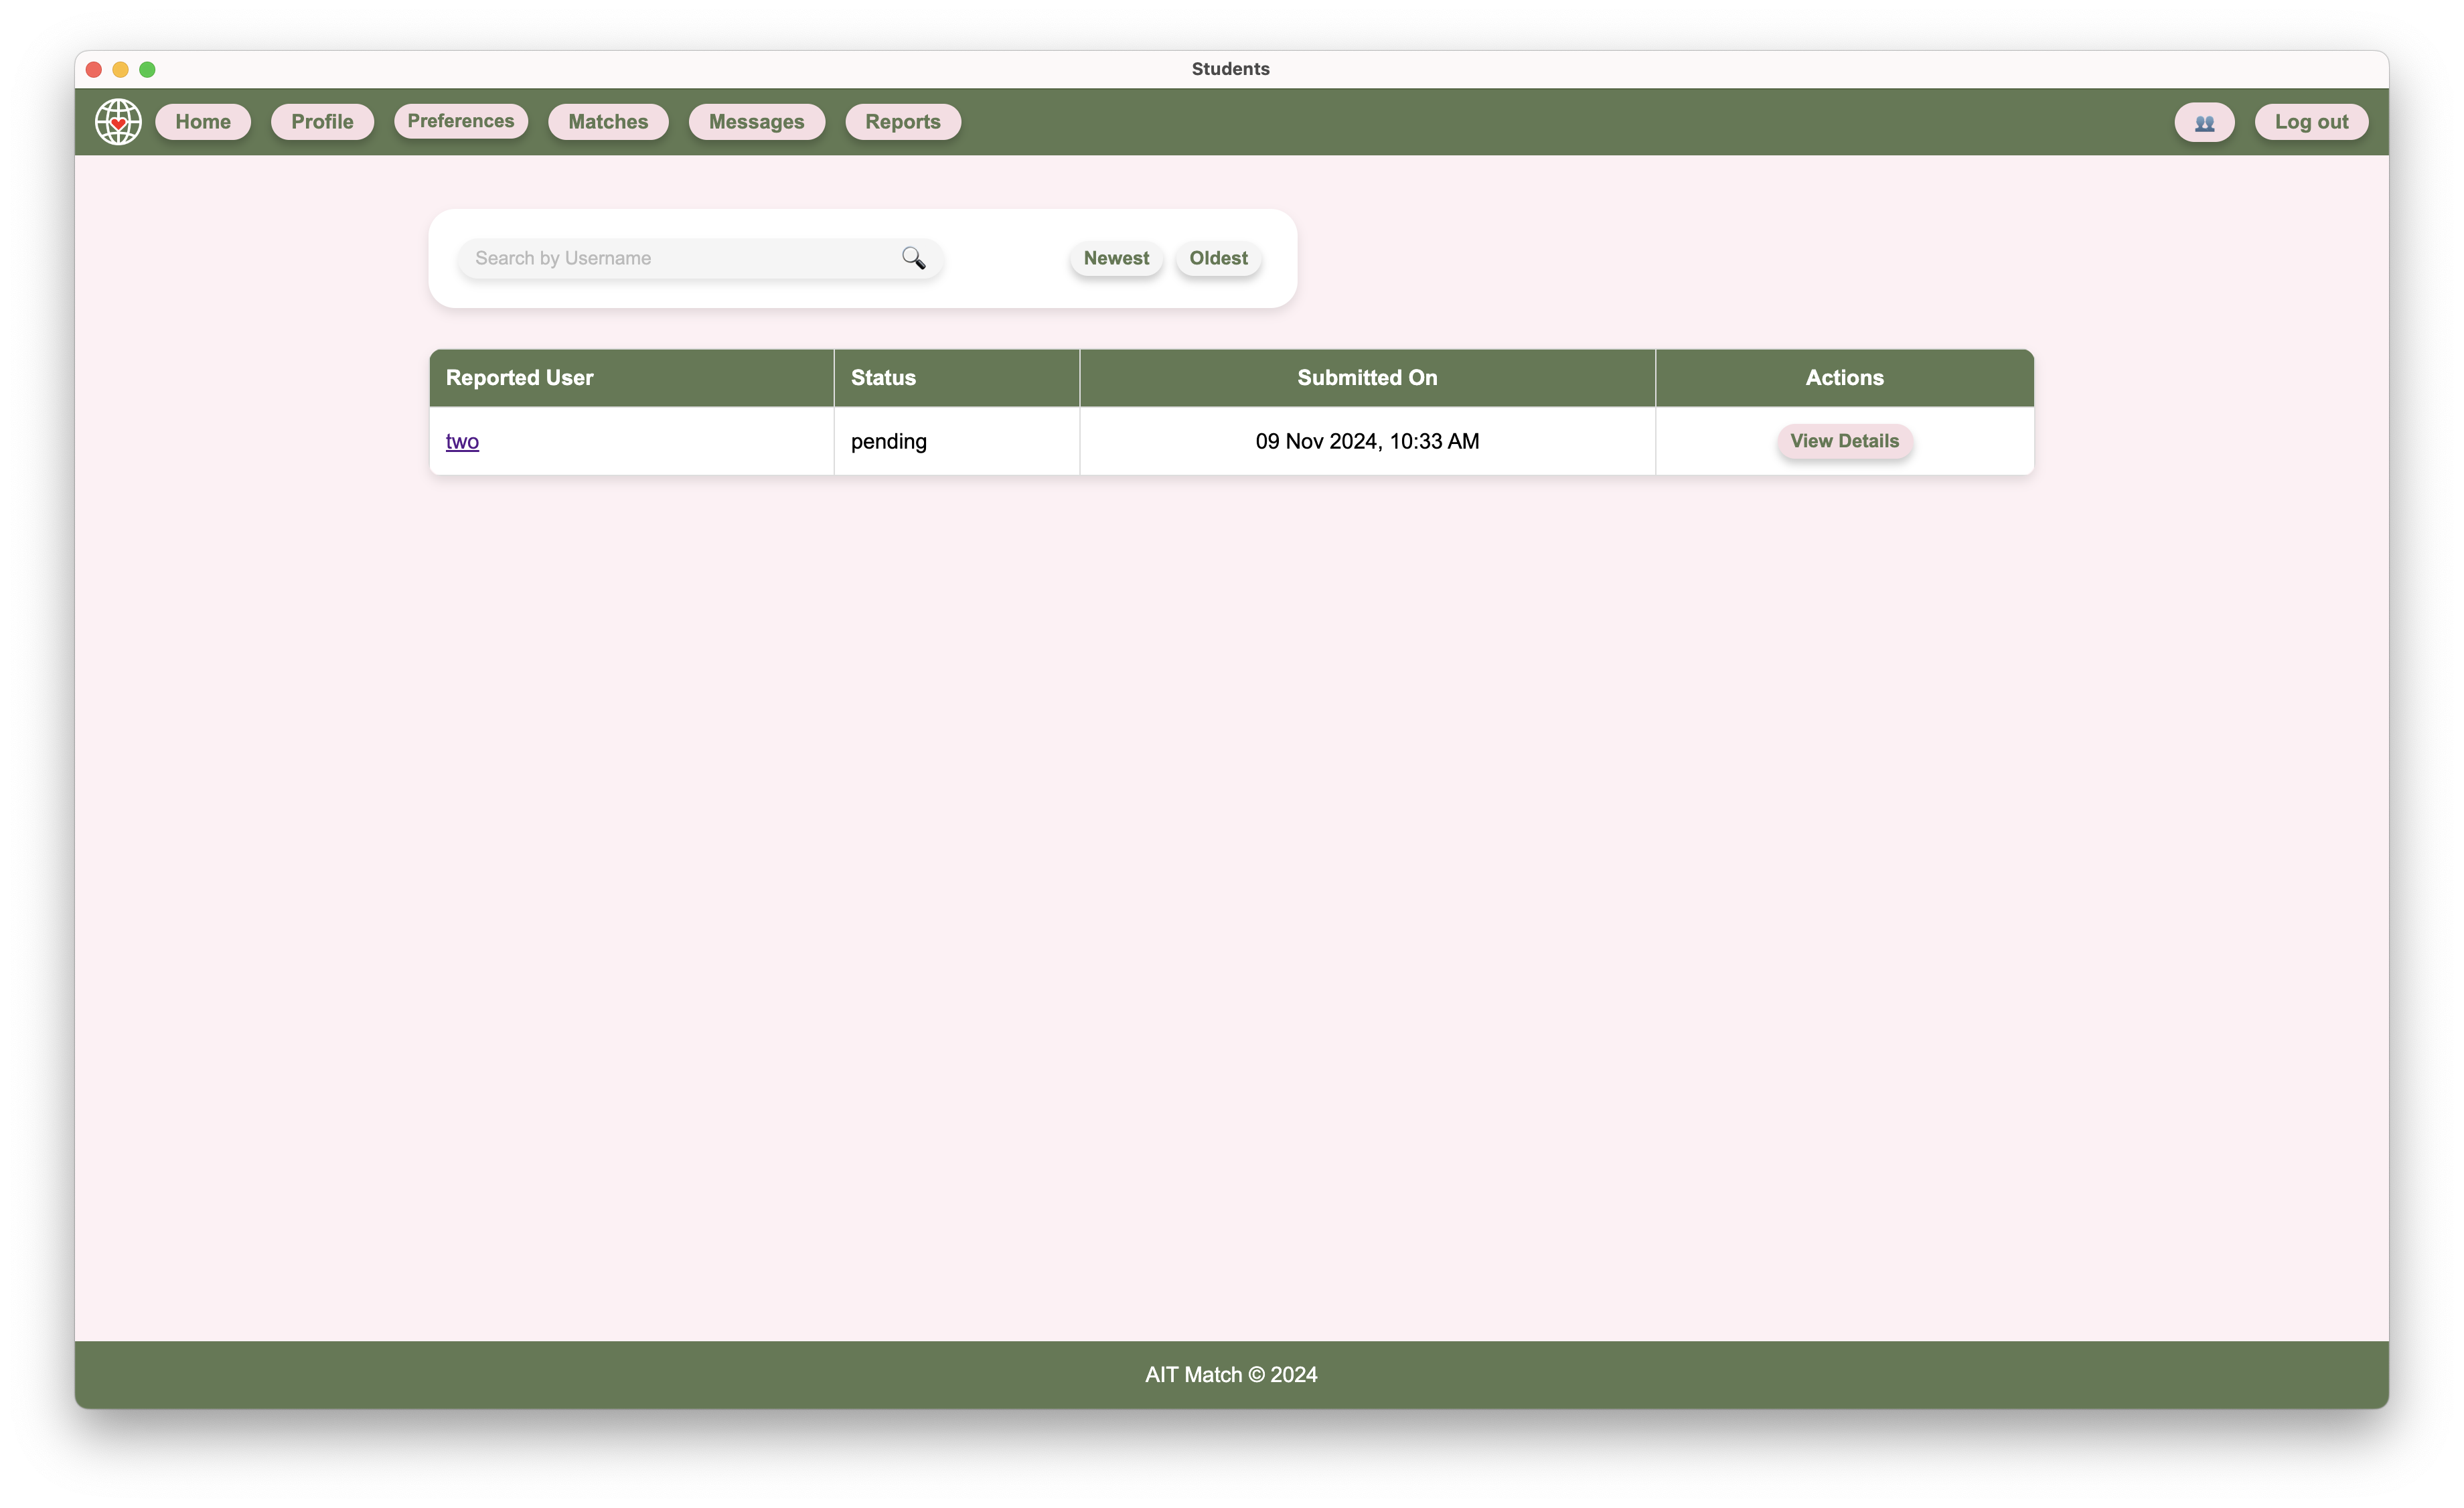
\includegraphics[width=5in]{figures/results/reports/report-index-page.png}
                \caption{Report Index Page.}
                \label{fig:report-index-page}
            \end{figure}

        \newpage
        \subsection{Report: Report Show Page}
        \begin{figure}[h]
                \centering
                \captionsetup{justification=centering, singlelinecheck=false, labelsep=space}
                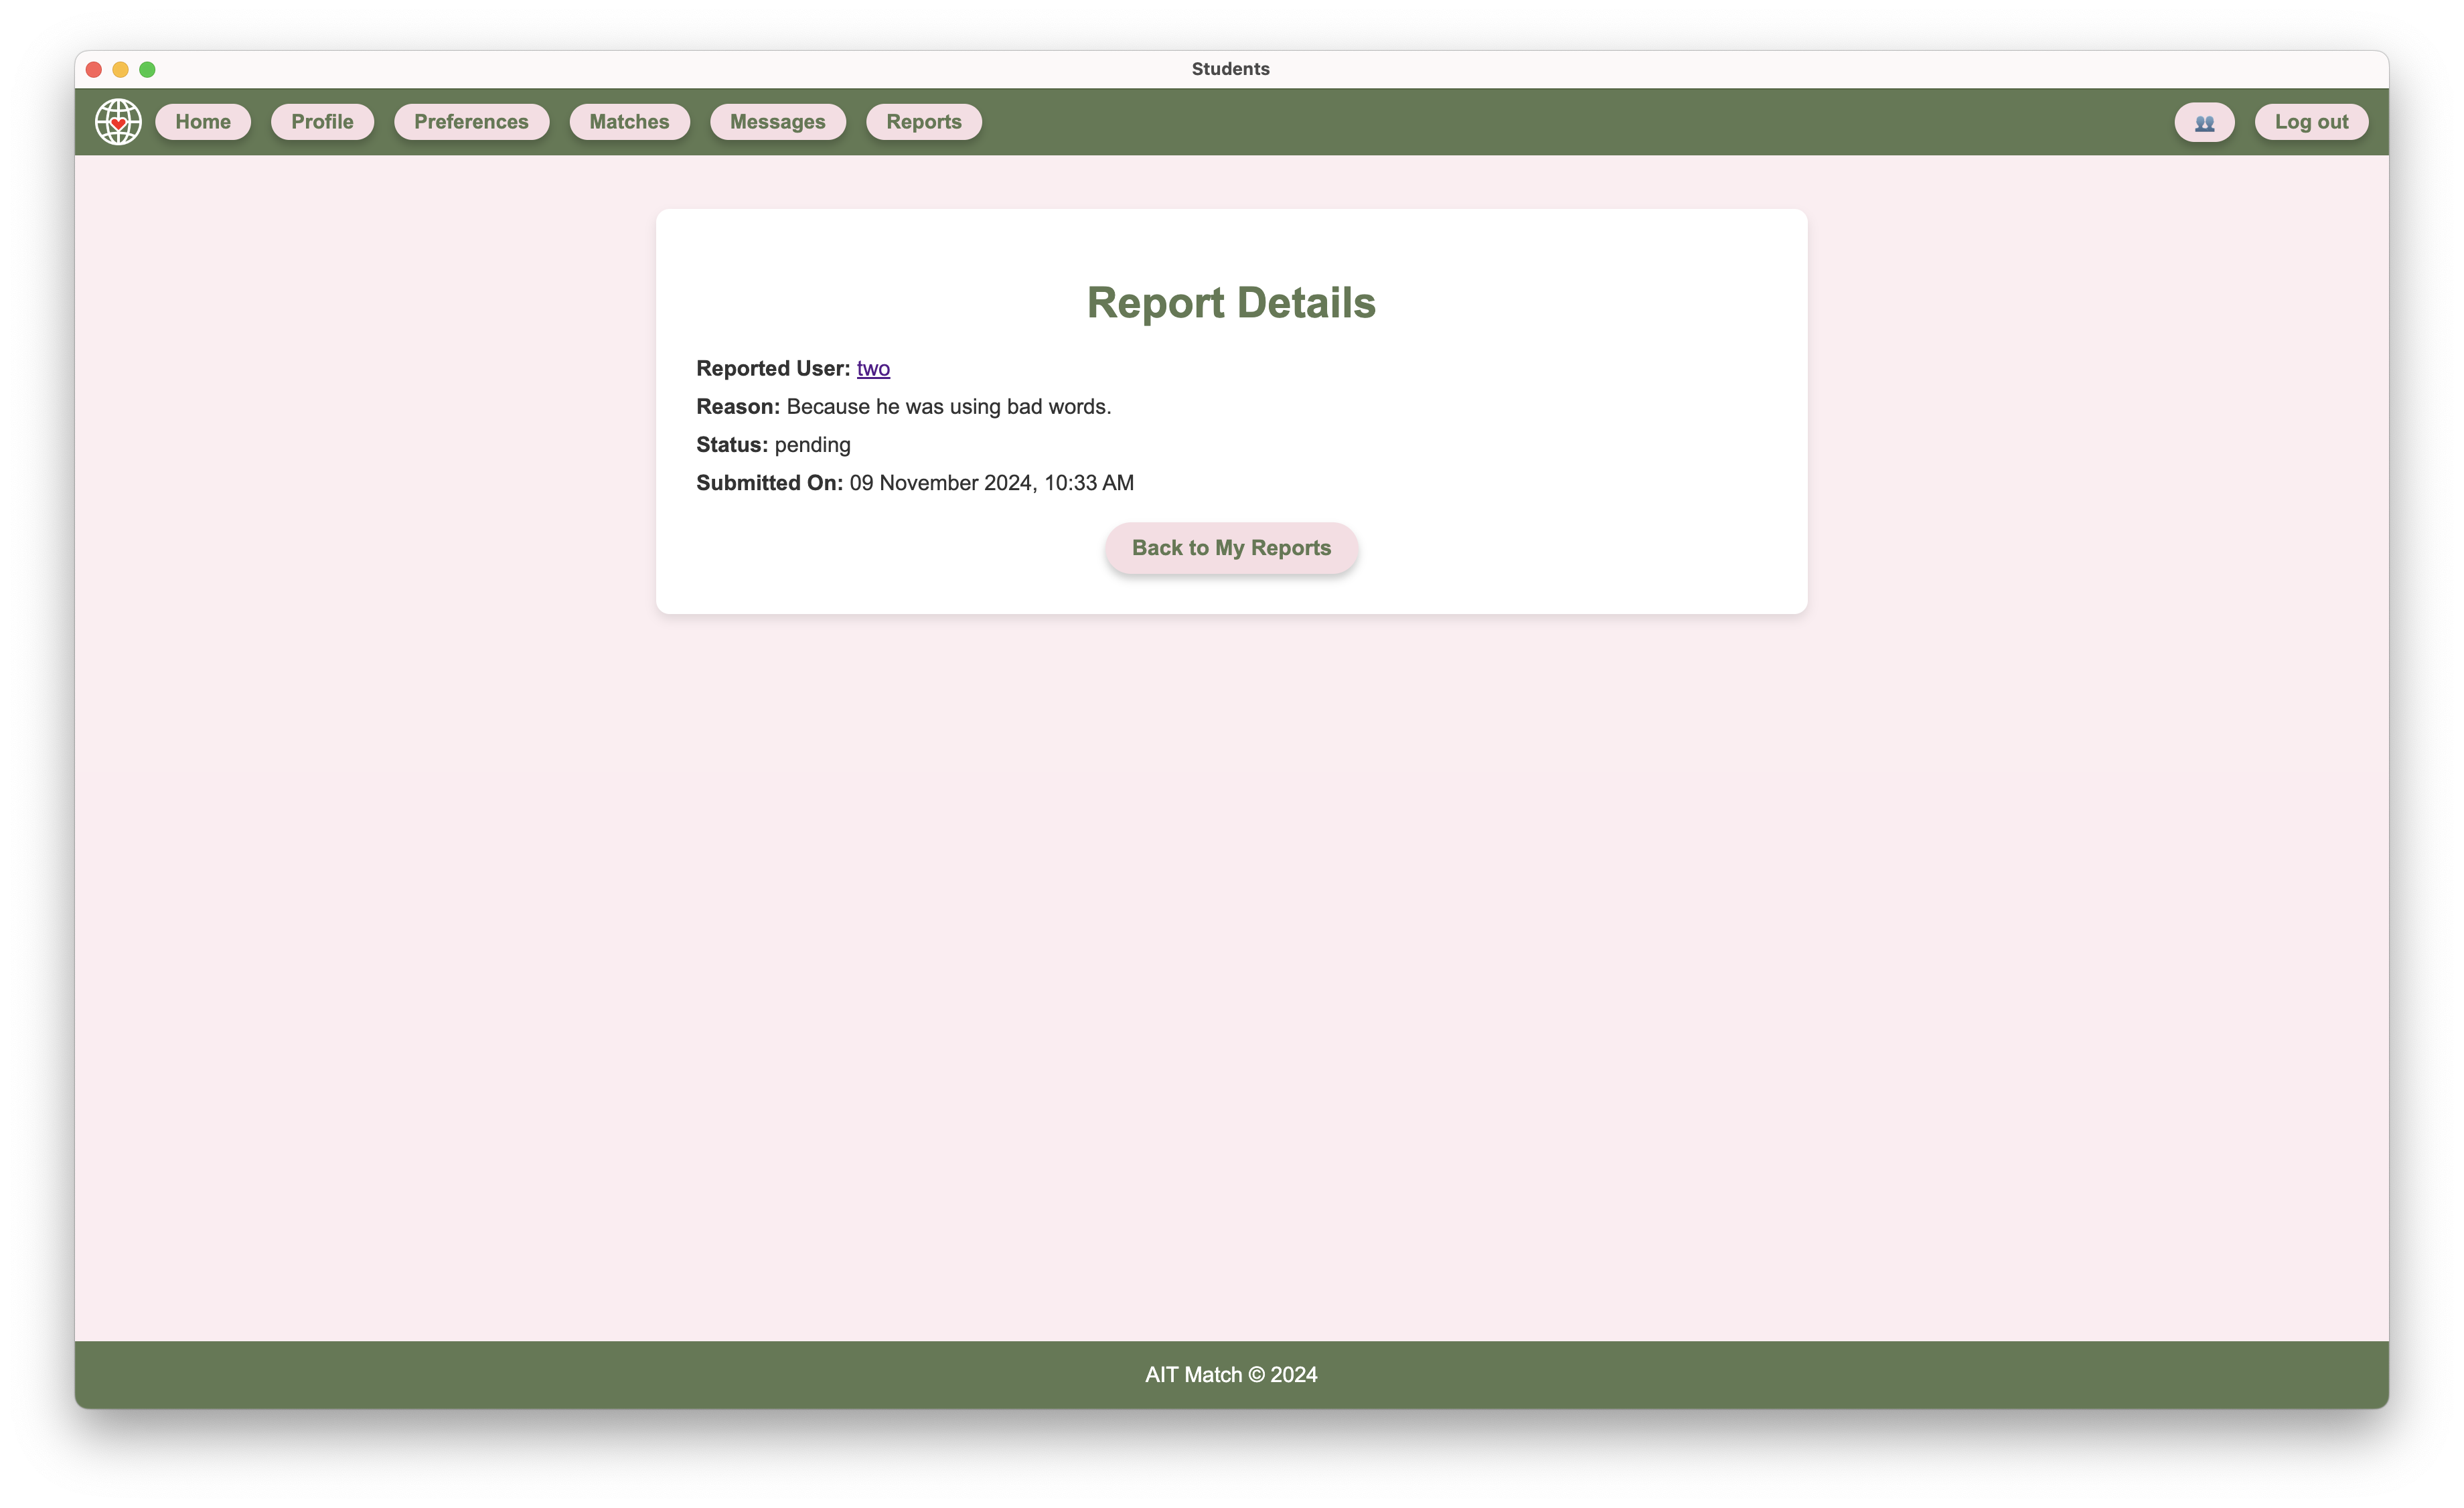
\includegraphics[width=5in]{figures/results/reports/report-show-page.png}
                \caption{Report Show Page.}
                \label{fig:report-show-page}
            \end{figure}
% ------------------------------------------------- %
        \newpage
        \subsection{Admin Panel: Users Management Page}
        \begin{figure}[h]
                \centering
                \captionsetup{justification=centering, singlelinecheck=false, labelsep=space}
                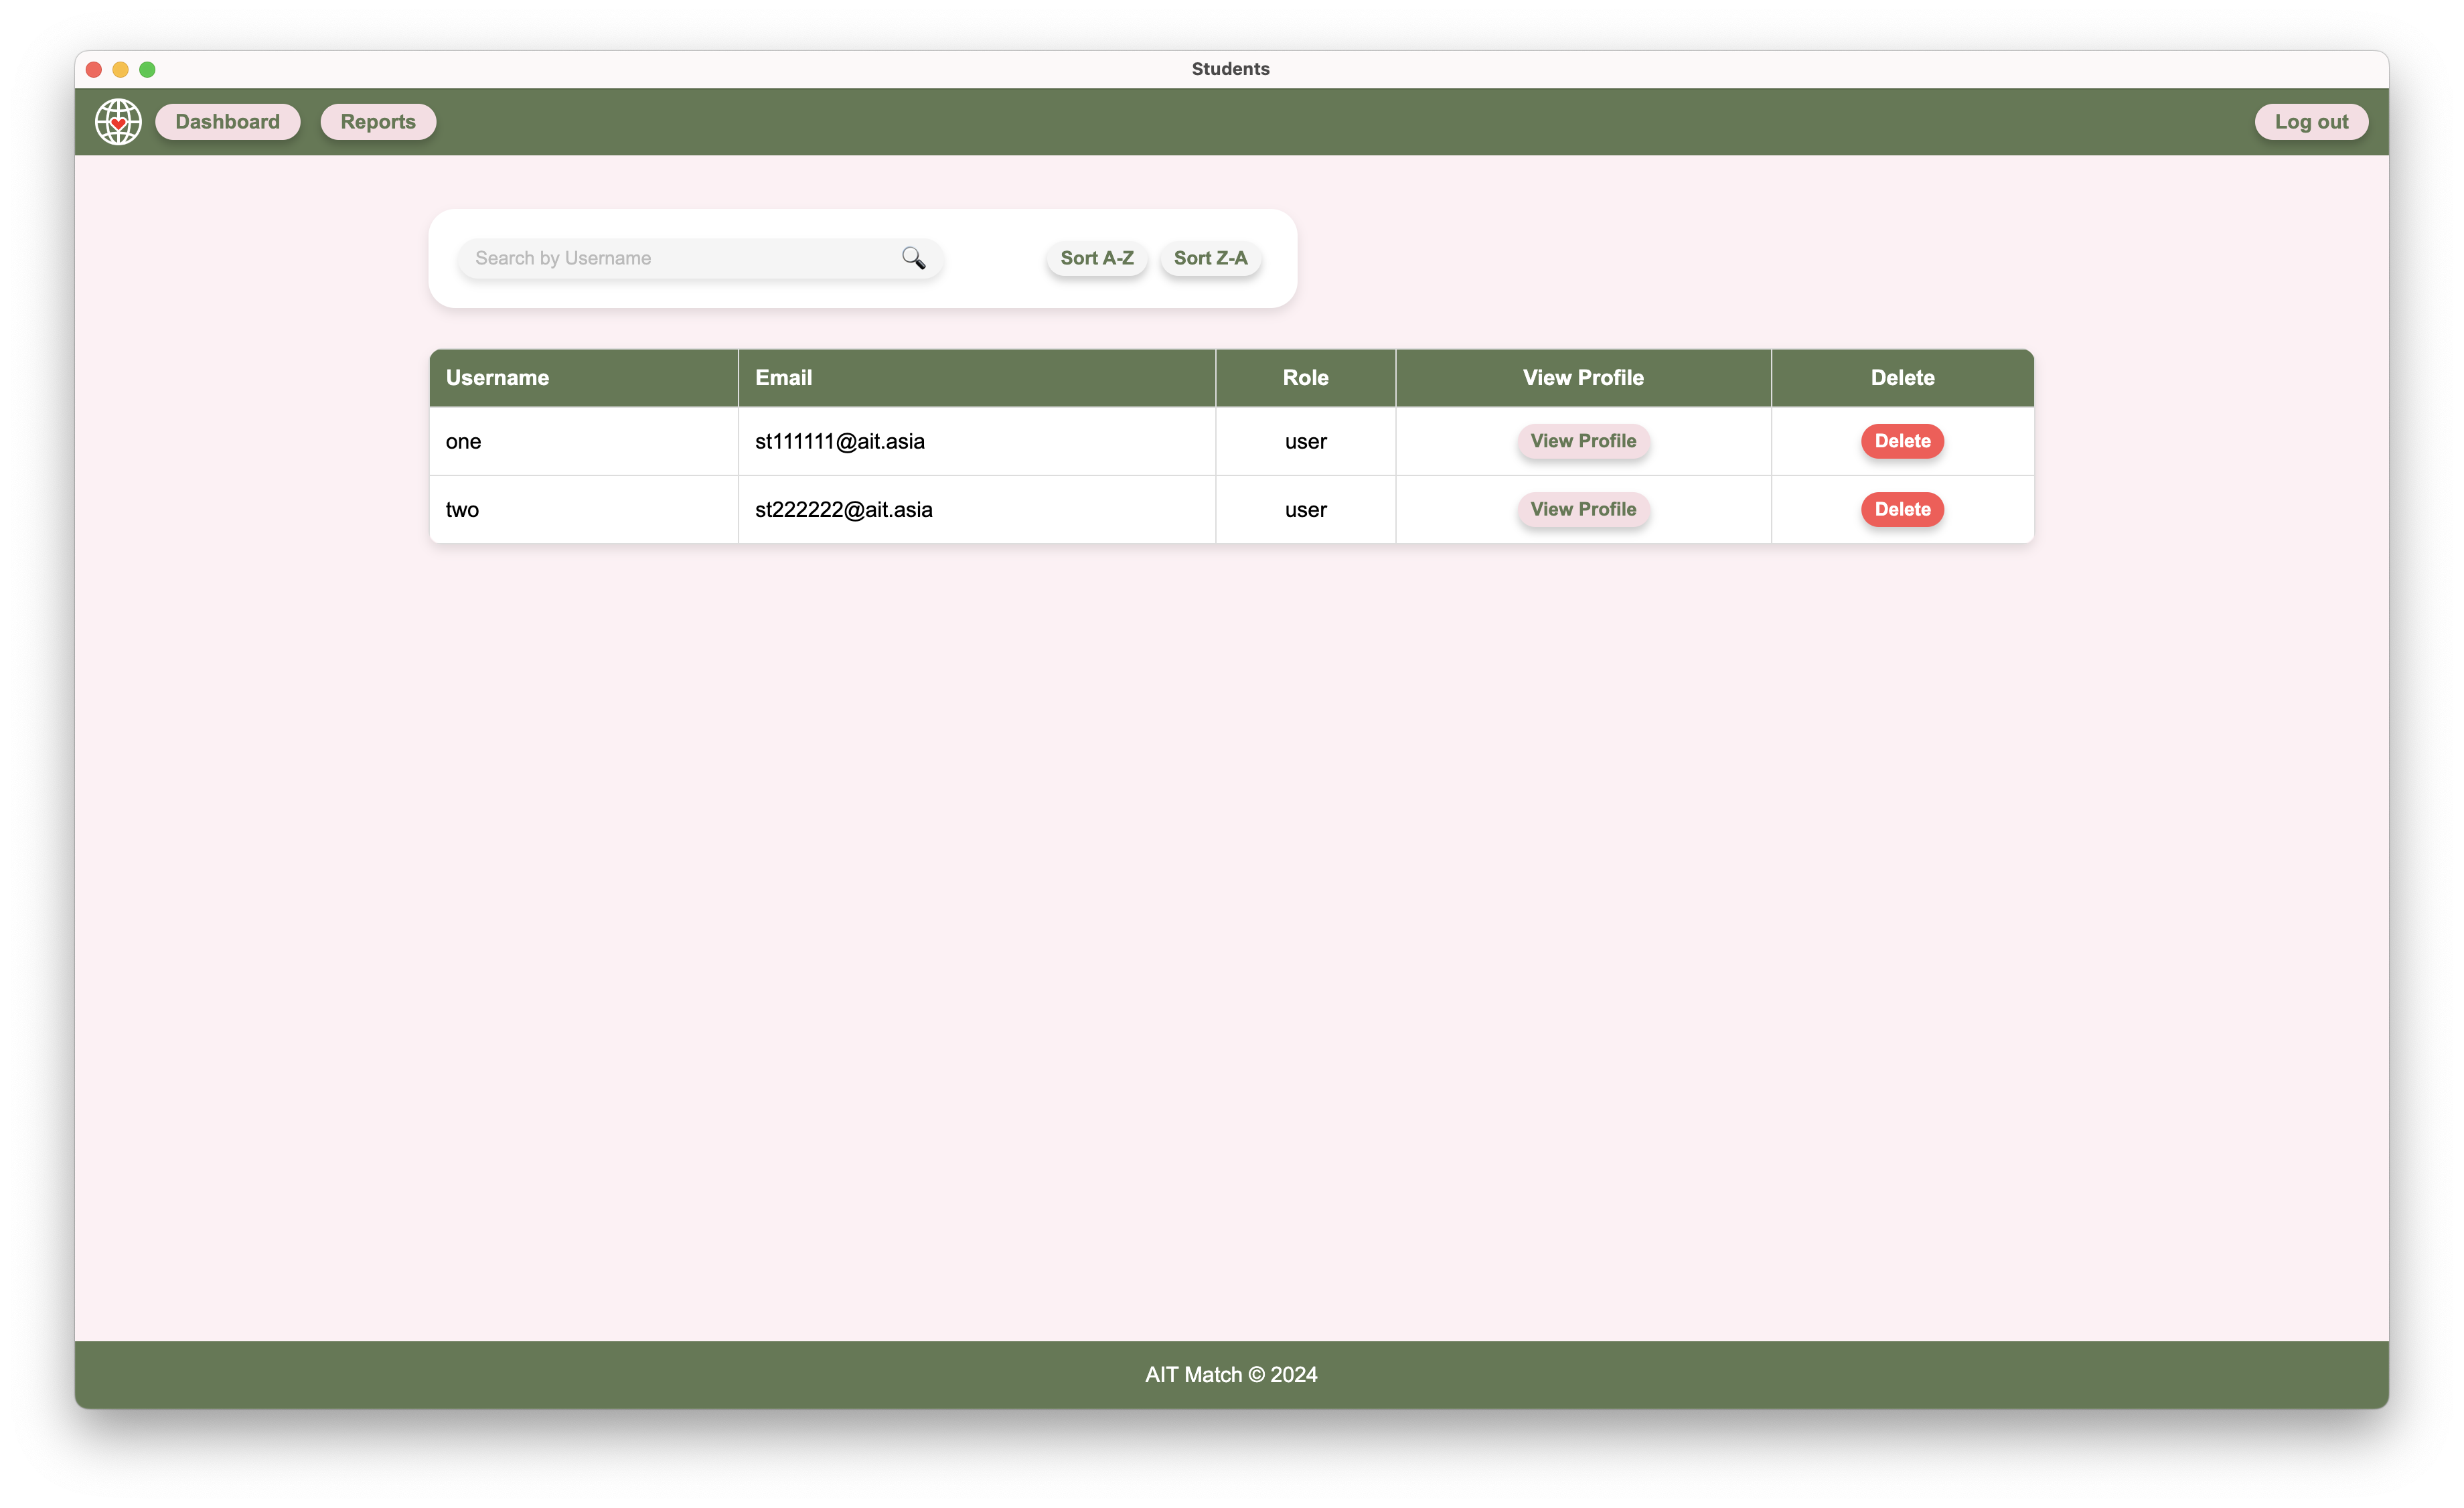
\includegraphics[width=5in]{figures/results/admin/user-management.png} 
                \caption{Admin Users Management Page.}
                \label{fig:user-management}
            \end{figure}

        \subsection{Admin Panel: Reports Management Page}
        \begin{figure}[h]
                \centering
                \captionsetup{justification=centering, singlelinecheck=false, labelsep=space}
                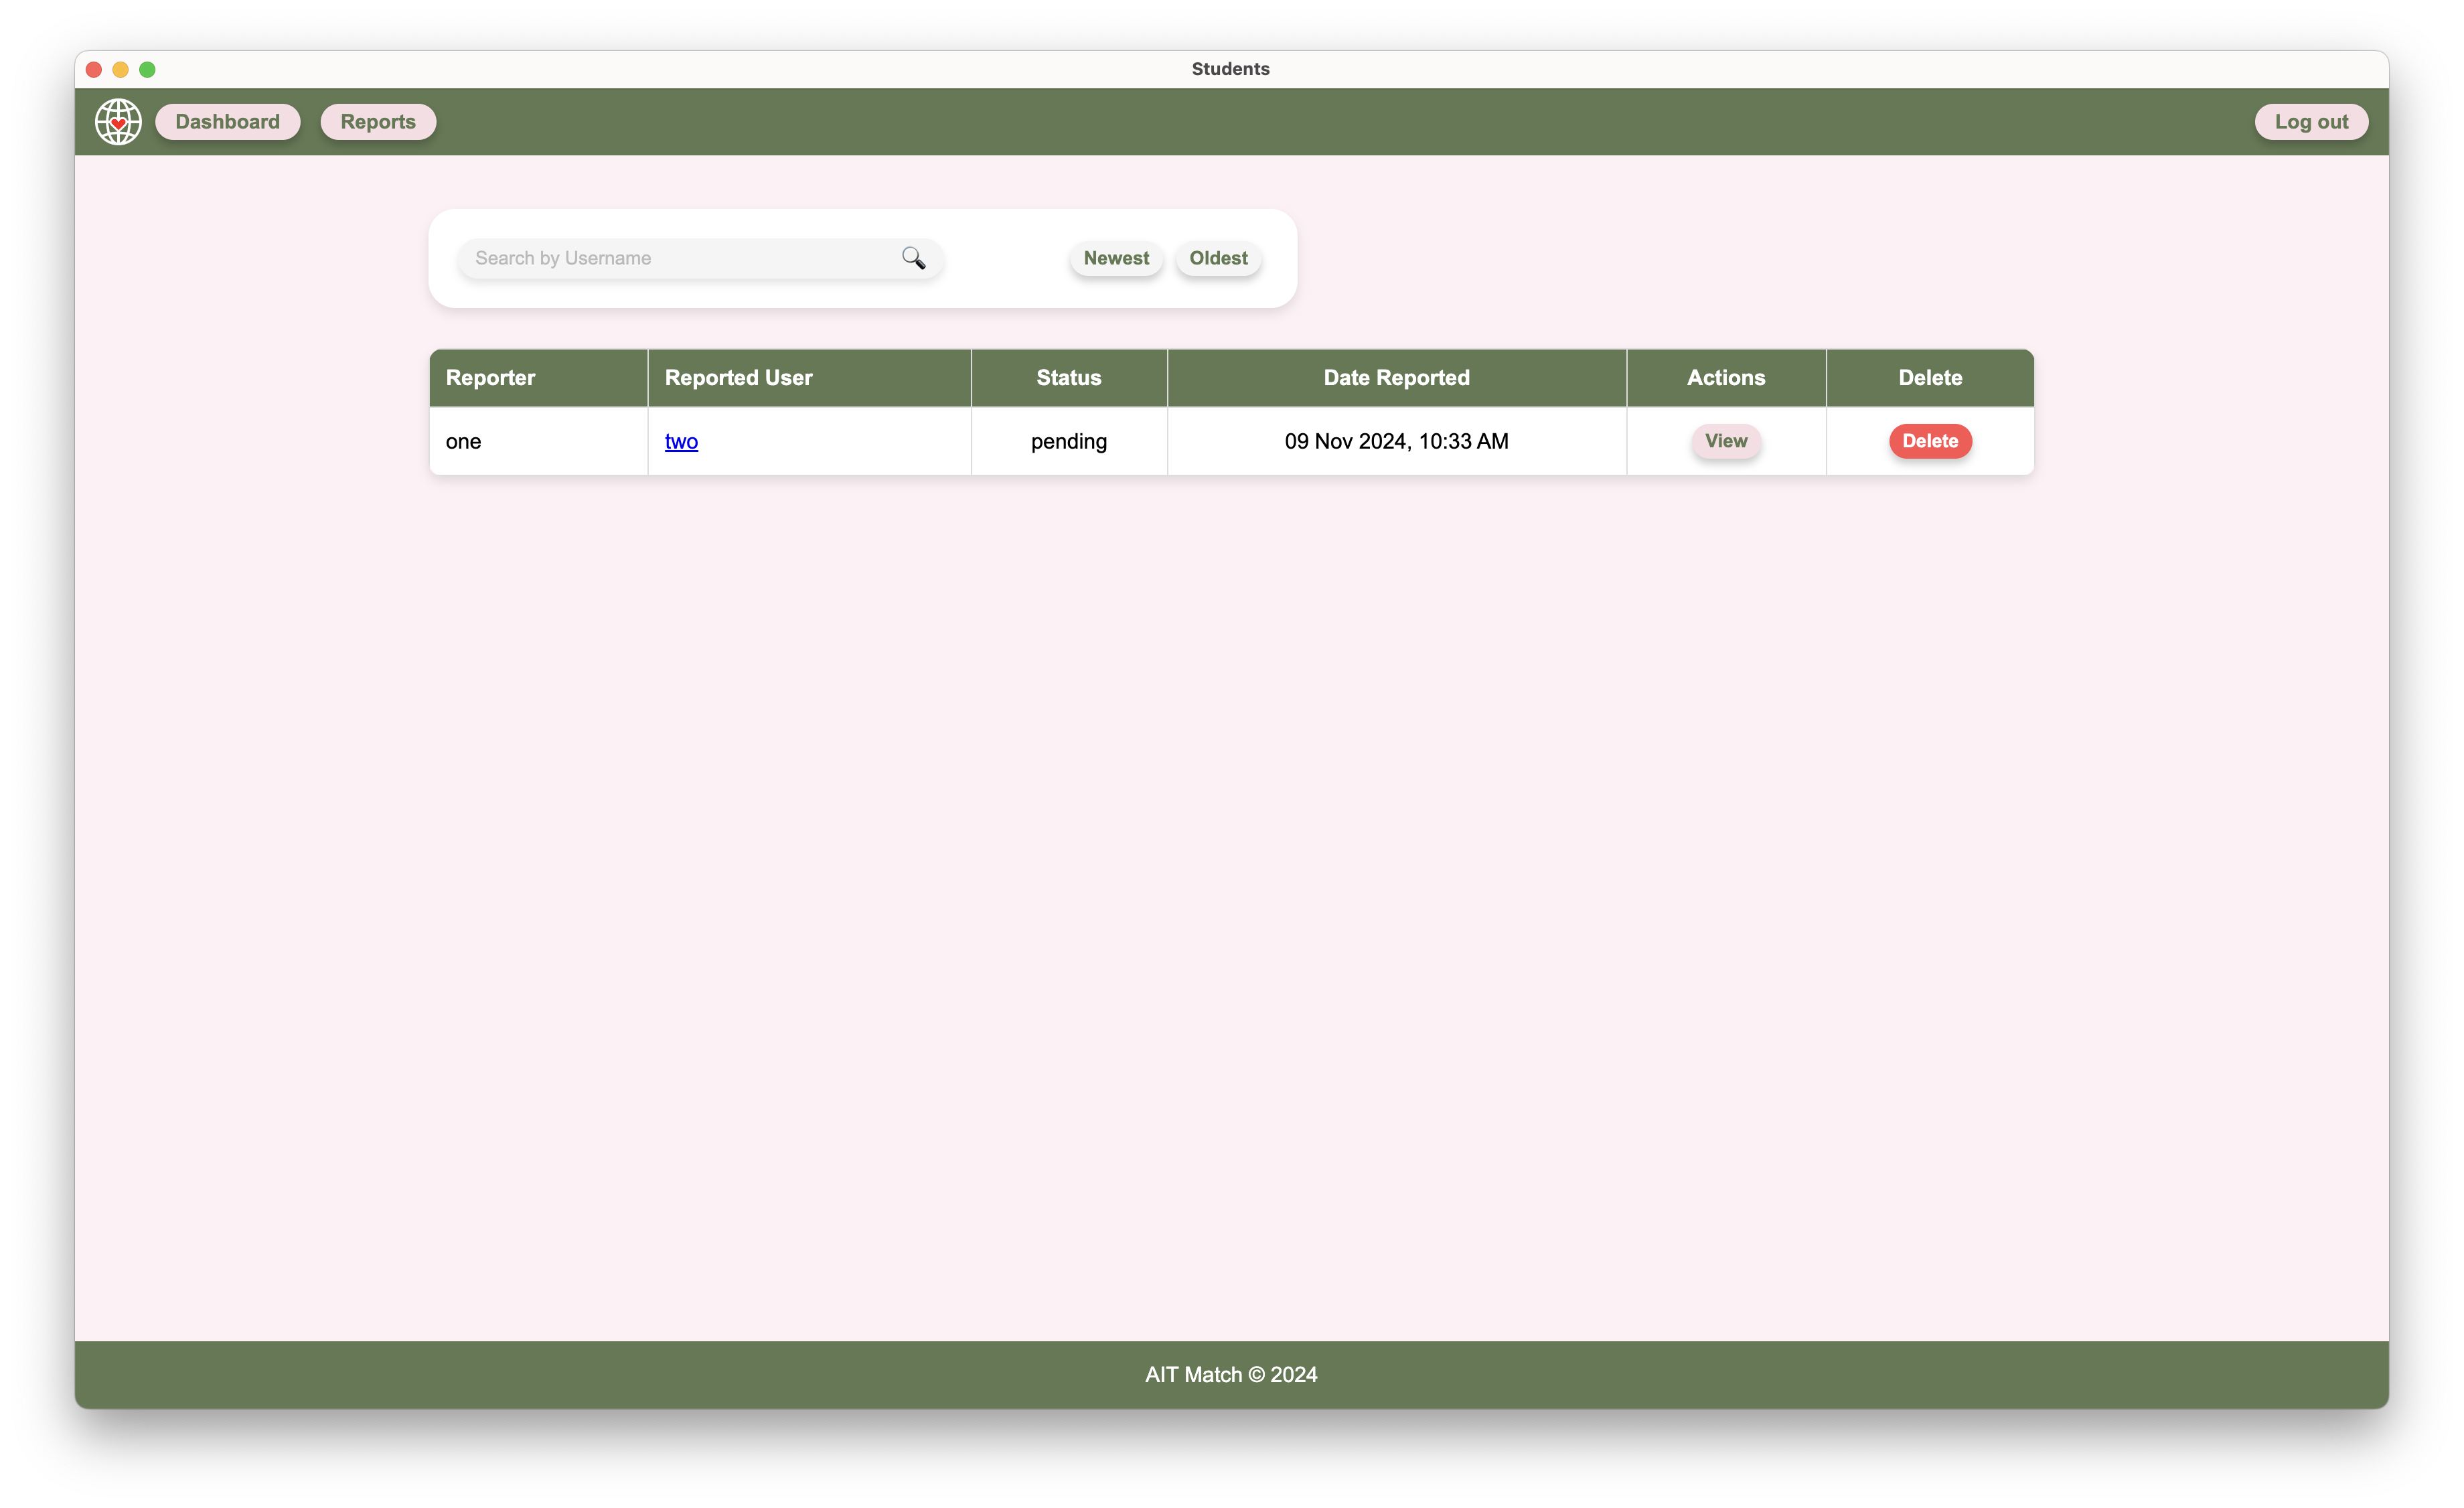
\includegraphics[width=5in]{figures/results/admin/report-management.png}
                \caption{Admin Reports Management Page.}
                \label{fig:report-management}
            \end{figure}

            



    \setlength{\footskip}{8mm}

\chapter{PROJECT EVALUATION}

\section{Challenges}
The development and deployment of the AIT Match application encountered several challenges, including:

    \subsection{Google Authentication and SMTP Email:} Integrating Google authentication and configuring SMTP for email notifications presented technical hurdles that required careful attention to security protocols. According to \cite{google_authentication}, as of September 30, 2024, Google will no longer support less secure apps that only use a username and password for authentication, particularly for Google Workspace accounts. This change means that using a simple username and password combination with SMTP to send emails from Gmail may no longer work due to the deprecation of this form of authentication for security reasons. Consequently, I faced significant challenges verifying my sender email for password resets in Devise, as this required adapting to new security measures that complicate the setup process for sending emails.
    
    \subsection{Google Drive Integration for Profile Pictures:}
    Initially, I attempted to use Google Drive links for hosting profile pictures; however, this proved to be impractical due to various restrictions imposed by Google, such as limitations on sharing and CORS (Cross-Origin Resource Sharing) policies, according to \cite{google_drive_restrictions}. Consequently, I shifted to using Imgur for image hosting. Unfortunately, this transition also presented challenges, particularly in a production environment where access is limited to the CSIM server via the CSIM Wi-Fi. This setup effectively blocks Imgur's IP addresses, preventing users from accessing images hosted on Imgur while using the application. As a result, I opted to implement Active Storage for image management, as it provides a more seamless user experience and circumvents these access issues.

    \newpage
    \subsection{ActiveStorage Performance Issues:} The implementation of ActiveStorage for managing user-uploaded images resulted in slower website performance. According to \cite{rails_active_storage}, this slowdown can be attributed to several factors, including the overhead associated with processing and storing images, which can lead to increased load times and reduced responsiveness of the application. Specifically, when images are uploaded, ActiveStorage needs to create multiple variants for different display requirements, which requires additional processing time and storage space. Moreover, the reliance on external storage services can introduce latency, especially if network conditions are suboptimal. These performance issues necessitated optimizations to ensure a smoother user experience

    \subsection{Performance Issues Due to Excessive Queries}
    One significant challenge encountered in the AIT Match platform is the slow performance of the website, particularly when handling user queries. The filtering system, which allows users to specify multiple criteria when searching for profiles, results in a large number of database queries. As users request more complex filters, the system performs additional queries to fetch the required data. This can lead to increased load times and reduced responsiveness, negatively impacting the overall user experience.
    
    Additionally, when users are setting up their profiles or preferences and need to fill in user information from the dataset in the database, the system also experiences slow performance. Retrieving and populating data from the database for these forms can further exacerbate load times, making the user experience cumbersome. Optimizing these queries and implementing more efficient data retrieval methods will be necessary to enhance the performance of the application.


\newpage
\section{Future Work}
In anticipation of continued growth and user engagement, several enhancements and new features are proposed to further improve the AIT Match platform:

\subsection{Expansion to Other Universities}
Plans are underway to broaden the platform's reach by making it available to students from other universities, thereby enhancing the user base and community engagement. Currently, the application is limited to users from the Asian Institute of Technology (AIT), but future developments could extend accessibility to other institutions across Thailand, facilitating a more diverse community of learners.

\subsection{User Ban System}
Developing a system to ban users instead of deleting their accounts provides a more flexible approach to managing user behavior. Currently, administrators can only delete profiles deemed inappropriate, which is a permanent action. By introducing a ban feature, administrators can temporarily restrict access to the chat function or place a user in a timeout for a designated period, allowing for corrective actions without permanently removing users from the platform.

\subsection{Filter Inappropriate Words in Chat}
Implementing filters to prevent users from typing inappropriate words in the chat system is essential for maintaining a respectful environment. This feature will actively screen messages to block any offensive language or derogatory terms, ensuring that all users can communicate in a safe and constructive manner.

\subsection{Chat Functionality between Users and Admin}
Enabling direct communication channels between users and administrators will significantly enhance support and user experience. Currently, users who submit reports have no means to inquire about the status or outcomes of their submissions. Likewise, administrators lack a mechanism to provide updates or feedback on the reports. Implementing a chat feature or comment section for each report will foster open communication, allowing users to seek clarifications and administrators to convey updates effectively.

\subsection{Addition of Events, Blogs, Posts, and Comments}
Integrating features for users to create and share events, blogs, posts, and comments will promote greater engagement and interaction within the community. This functionality would empower users to contribute to discussions, share experiences, and foster a lively social atmosphere, making the platform not just a dating app but also a hub for community interaction.

\subsection{More Customizable Interests}
Allowing users to define a wider range of customizable interests will enhance matching accuracy and user satisfaction. At present, users can only select from preset options defined by developers, which may not fully capture their unique preferences. Future iterations should incorporate features that allow users to add and modify their interests, leading to more tailored connections and experiences.

\subsection{Chat with Sending Images and Emojis}
Currently, the chat functionality is limited to text messaging, which may feel monotonous for users. Future updates could include support for sending images and emojis, making conversations more dynamic and engaging. This enhancement would allow users to express themselves more fully and interact in a fun, creative manner, thereby enriching the overall chat experience.
 
    %   \begin{center}
%     \large{\bf AUTHOR'S DECLARATION}
% \end{center}

%   I, NAME, declare that the research work carried out for this thesis was in accordance with the regulations of the Asian Institute of Technology. The work presented in it are my own and has been generated by me as the result of my own original research, and if external sources were used, such sources have been cited. It is original and has not been submitted to any other institution to obtain another degree or qualification. This is a true copy of the thesis including final revisions.

%   Date: April 18, 2022

%   Name: 

%   \vspace{-3em}\hspace{4em}\includegraphics*[height=30pt]{figures/name.png}

%   Signature: 

%   \vspace{-3em}\hspace{5.5em}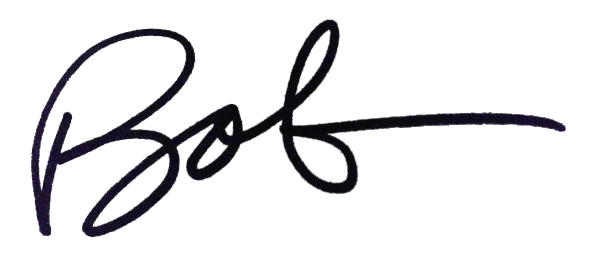
\includegraphics[height=30pt]{figures/signature.png}

    % \newpage
% \phantomsection
% \addcontentsline{toc}{chapter}{\bf LIST OF TABLES}
% \addtocontents{lot}{\textbf{Tables}\hfill\textbf{Page}\par}
% \listoftables

% \newpage
% \phantomsection
% \addcontentsline{toc}{chapter}{\bf LIST OF FIGURES}
% \addtocontents{lof}{\textbf{Figures}\hfill\textbf{Page}\par}
% \listoffigures
    
    \pagestyle{plain}  
    
    \newpage
    \phantomsection
    \addcontentsline{toc}{chapter}{\bf REFERENCES}
    \bibliography{references}    
    \newpage\pagestyle{plain}
    % \appendix
% \renewcommand{\appendixname}{APPENDIX}
% \captionsetup[table]{labelfont=bf,name=Table\space,labelsep=space}
% \captionsetup[figure]{labelfont=bf,name=Figure\space,labelsep=space}
% \renewcommand\thefigure{\thechapter\arabic{figure}} 
% \newcommand{\stoptocwriting}{%
%   \addtocontents{toc}{\protect\setcounter{tocdepth}{-5}}}
% \newcommand{\resumetocwriting}{%
%   \addtocontents{toc}{\protect\setcounter{tocdepth}{\arabic{tocdepth}}}}

% \captionsetup{
%   singlelinecheck=false,
%   textfont=bf
% }

% \newpage
% \phantomsection
% \addcontentsline{toc}{chapter}{\bf APPENDICES}
% \begin{center}
%     \vspace*{\fill}
%     \large{\bf APPENDICES}
%     \vspace*{\fill}
% \end{center}
% \newpage

% \phantomsection
% \addcontentsline{toc}{section}{\bf \uppercase{APPENDIX A: TITLE}}
% \stoptocwriting
% \chapter{\uppercase{TITLE}}
% \resumetocwriting

% \begin{figure}[h]
% \caption{Doge.}
% \centerline{\includegraphics[width=3in]{figures/doge.jpeg}}
% \label{fig:doge2}
% \small{\textit{Note.} Notice the different styling of figures in the appendix...}
% \end{figure}


\end{document}
